\documentclass[aspectratio=169, usenames, dvipsnames]{beamer}
\usetheme{metropolis}
\metroset{block=fill}

\usepackage{newpxtext}
\usepackage{newpxmath}

\usepackage{amsmath}
\usepackage{graphicx}
\usepackage{physics}
\usepackage{ragged2e}
\usepackage{filecontents}
\usepackage{xcolor}

\usepackage[binary-units]{siunitx}
\DeclareSIUnit\flops{FLOPS}
\DeclareSIUnit\year{yr}

\usepackage{pgfplots}
\pgfplotsset{width=\textwidth, height=0.494427\textwidth}


\usepackage{tikz}
\usepackage{mathtools}
\usetikzlibrary{positioning, shapes.geometric, arrows, arrows.meta, spy, shadows, mindmap, calc}
\usepgfplotslibrary{colorbrewer}

\usefonttheme{serif}

\title{Optically-Active Media}
\subtitle{The QuEST for light-matter models}
\date{December 20, 2017}
\author{Connor Glosser}
\institute{Michigan State University}

\newcommand{\oper}[1]{\mathcal{#1}}
\newcommand{\rwoper}[1]{\tilde{\mathcal{#1}}}
\newcommand{\outerprod}[2]{#1 \! \otimes \! #2}

\begin{document}

\maketitle

\section{Computational electromagnetics}

\begin{frame}{Why (computational) electromagnetics?}
  \begin{columns}
    \column{0.5\textwidth}
      \begin{itemize}
        \item Maxwell's equations govern electromagnetic phenomena
          \begin{itemize}
            \item Radar, antennas, optics, telecommunications, \ldots
          \end{itemize}
        \item Analytic solutions unavailable for all but simplest geometries
        \item Simulate!
          \begin{itemize}
            \item How to represent \emph{equations} discretely?
            \item How to represent \emph{boundary conditions} discretely?
            \item Algorithmic complexity?
            \item Precision?
          \end{itemize}
      \end{itemize}
    \column{0.5\textwidth}
    \begin{center}
      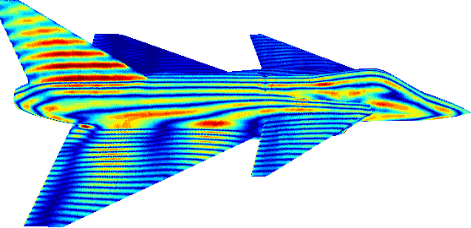
\includegraphics[width=0.7\textwidth]{figures/aircraft}
      \vspace{0.3cm}
      \begin{block}{Maxwell's equations}
        \begin{gather*}
          \div \vb{E} = 4 \pi k_1 \rho \qquad \curl \vb{E} = -k_3 \pdv{\vb{B}}{t} \\
          \curl \vb{B} = 4 \pi k_2 \alpha \vb{J} + \frac{k_2 \alpha}{k_1} \pdv{\vb{E}}{t} \qquad \div \vb{B} = 0
        \end{gather*}
      \end{block}
    \end{center}
  \end{columns}
\end{frame}

\begin{frame}{Problem statement}
  Given
  \begin{center}
    geometry, material data, excitation, incident field
  \end{center}
  determine
  \begin{center}
    near and far fields, impedances, coupling
  \end{center}
  in the
  \begin{center}
    time or frequency domain.
  \end{center}
\end{frame}

\begin{frame}{The computational electromagnetics toolbox}
  \begin{center}
    %This figure requires both the shadows and mindmap tikzlibraries. Include them in your header!
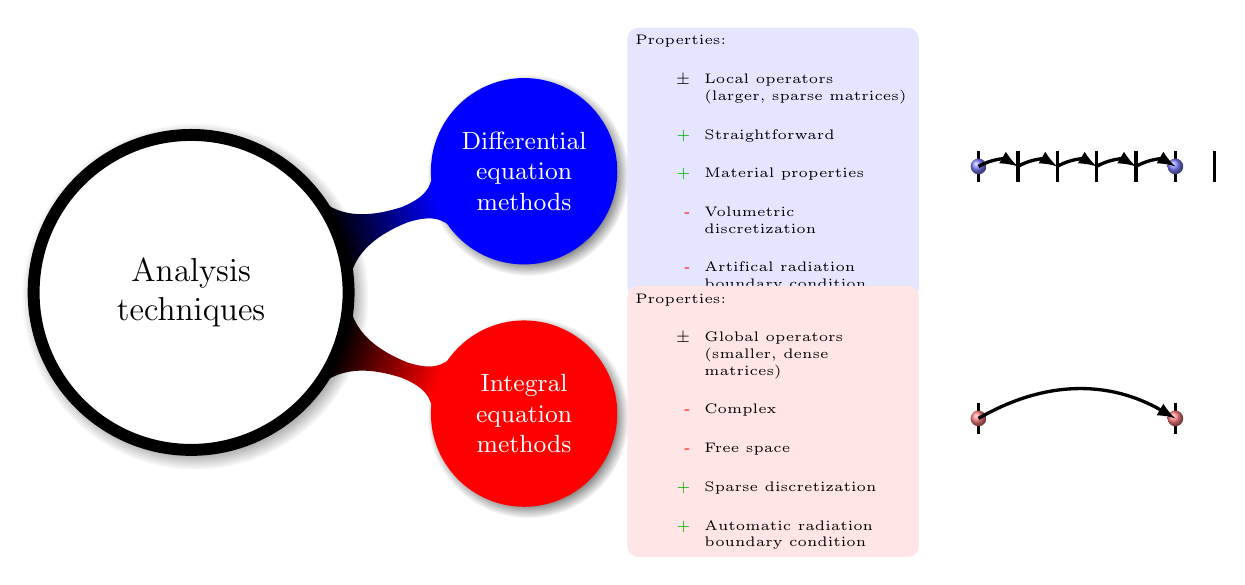
\begin{tikzpicture}[mindmap, >=latex]
  \begin{scope}[
    every node/.style={concept, circular drop shadow,execute at begin node=\hskip0pt},
    root concept/.append style={
      concept color=black, fill=white, line width=1ex, text=black
    },
    text=white,
    IE/.style={concept color=red,faded/.style={concept color=red!50}},
    DE/.style={concept color=blue,faded/.style={concept color=blue!50}},
    measuring complexity/.style={concept color=orange,faded/.style={concept color=orange!50}},
    solving problems/.style={concept color=green!50!black,faded/.style={concept color=green!50!black!50}},
    grow cyclic,
    level 1/.append style={level distance=4.5cm, sibling angle=40},
    level 2/.append style={level distance=3cm,sibling angle=30}]

  \node[root concept]{Analysis techniques}
  child[IE]{ node (IE) {Integral equation methods}}
  child[DE]{ node (DE) {Differential equation methods}};
    \end{scope}
  \begin{scope}[every annotation/.style={fill=blue!10}]
    \node [annotation, xshift=2cm, yshift=0.1cm] at (DE.east) {
      Properties:
       \begin{itemize}
         \item[$\pm$] Local operators \\ (larger, sparse matrices)
         \item[\textcolor{green!70!black}{+}] Straightforward
         \item[\textcolor{green!70!black}{+}] Material properties
         \item[\textcolor{red}{-}] Volumetric discretization
         \item[\textcolor{red}{-}] Artifical radiation boundary condition
       \end{itemize}
    };
  \end{scope}
  \begin{scope}[every annotation/.style={fill=red!10}]
    \node [annotation, xshift=2cm, yshift=-0.1cm] at (IE.east) {
      Properties:
       \begin{itemize}
         \item[$\pm$] Global operators \\ (smaller, dense matrices)
         \item[\textcolor{red}{-}] Complex
         \item[\textcolor{red}{-}] Free space
         \item[\textcolor{green!70!black}{+}] Sparse discretization
         \item[\textcolor{green!70!black}{+}] Automatic radiation boundary condition
       \end{itemize}
    };
  \end{scope}

  \foreach \x in {10,10.5,...,13}
    \draw (\x, 1.4) -- (\x, 1.8);

  \shade [ball color=blue!50] (10, 1.6) circle [radius=0.1cm];
  \shade [ball color=blue!50] (12.5, 1.6) circle [radius=0.1cm];

  \draw[->] (10.0, 1.6) to[out=30, in=150] (10.5, 1.6);
  \draw[->] (10.5, 1.6) to[out=30, in=150] (11.0, 1.6);
  \draw[->] (11.0, 1.6) to[out=30, in=150] (11.5, 1.6);
  \draw[->] (11.5, 1.6) to[out=30, in=150] (12.0, 1.6);
  \draw[->] (12.0, 1.6) to[out=30, in=150] (12.5, 1.6);

  \draw (10,-1.4) -- (10, -1.8);
  \draw (12.5,-1.4) -- (12.5, -1.8);

  \shade [ball color=red!50] (10, -1.6) circle [radius=0.1cm];
  \shade [ball color=red!50] (12.5, -1.6) circle [radius=0.1cm];

  \draw[->] (10, -1.6) to[out=30, in=150] (12.5, -1.6);
\end{tikzpicture}

  \end{center}
\end{frame}

\begin{frame}{Integral equations}
  \begin{columns}
    \column{0.6\textwidth}
    \begin{block}{Convolutional operator}
      \begin{equation*}
        \vb{E}(\vb{r}, t) = \vb{E}_\text{inc}(\vb{r}, t) + \mathcal{L}\qty{\vb{J}(\vb{r}, t)}
      \end{equation*}
      \hfill \tiny{(applies to lots of physical potentials)}
    \end{block}

    \begin{block}{Discretized unknown quantity}
      \begin{equation*}
        \vb{J}(\vb{r}, t) \approx \sum_{t=1}^{N_t} \sum_{s=1}^{N_s} a_{ts} \, f_{ts}(\vb{r}, t)
      \end{equation*}
      \begin{itemize}
        \item $N_t, N_s \propto \omega_\text{max}, \omega_\text{max}^2$
        \item Cost to evaluate $\mathcal{L}\qty{\vb{J}(\vb{r}, t)} \sim \mathcal{O}(N_t N_s^2)$
      \end{itemize}
    \end{block}

    \column{0.4\textwidth}
      \begin{center}
        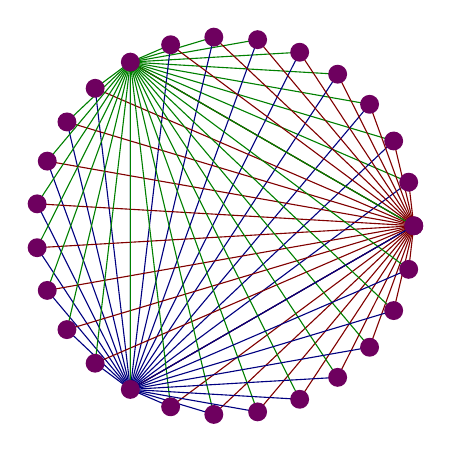
\begin{tikzpicture}[scale=0.8]
  \pgfmathsetmacro{\dtheta}{13.3333};

  \pgfmathsetmacro{\dthetaGrand}{9*\dtheta};
  \pgfmathsetmacro{\firstpt}{0};
  \pgfmathsetmacro{\secondpt}{\dthetaGrand};
  \pgfmathsetmacro{\thirdpt}{2*\dthetaGrand};

  \foreach \angle in {0, \dtheta, ..., 360}{
    \draw[red!50!black] (\firstpt:3) -- (\angle:3);
    \draw[green!50!black] (\secondpt:3) -- (\angle:3);
    \draw[blue!50!black] (\thirdpt:3) -- (\angle:3);
  }

  \pgfmathsetmacro{\nodeRadius}{0.15};
  \definecolor{level0}{RGB}{110,0,95}
  \foreach \angle in {0, \dtheta, ..., 360}{
    \draw[draw=none, fill=level0] (\angle:3) circle (\nodeRadius);
  }
\end{tikzpicture}

      \end{center}
  \end{columns}
\end{frame}

\begin{frame}{More perspective}
  \begin{itemize}
    \item Electrically large objects: $N_s > 10^6$
    \item Memory required $\sim \mathcal{O}(N_s^2) \approx \SI{8}{\tera\byte}$
    \item Time required
      \begin{itemize}
        \item Potential evaluation: $\mathcal{O}(N_s^2) \to \SI{1}{\hour}$ (at \SI{300}{\mega\flops})
        \item Full solution: $N_t \propto N_s$ so $\mathcal{O}(N_s^3) \to \SI{105}{\year}$
      \end{itemize}
  \end{itemize}
  \begin{block}{Goal}
    \begin{center}
      Develop methods that scale as $\mathcal{O}(N_s \log^\alpha N_s)$.
    \end{center}
    By exploiting physical and mathematical structure of the problem, we can develop formulations amenible to acceleration with controllable error.
  \end{block}
\end{frame}

\section{Fast methods}

\begin{frame}{Nonlinear quantum optics}
  \begin{itemize}
    \item Liouville equation: $\partial_t \hat{\rho}(\vb{r}, t) = f\qty\big(\hat{\rho}(\vb{r}, t), \vb{E}(\vb{r}, t))$
      \begin{itemize}
        \item $\hat{\rho}$ characterizes $\vb{J}$ directly
        \item Dynamical absorption, emission
        \item Discretization based on ODE frequency
        \item Introduction of nonlinear sources, $\vb{P} \not = \chi_e \vb{E}$
        \item Reconcile with Maxwell's equations; simultaneously solve both
      \end{itemize}
  \end{itemize}
  \begin{center}
    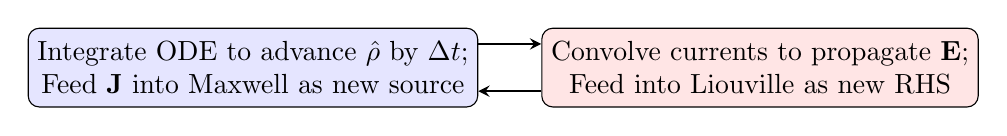
\begin{tikzpicture}[node distance=0.8cm, >=latex]
      \tikzstyle{physics} = [rectangle, rounded corners, minimum width=3cm, minimum height=1cm,text centered, draw=black, fill=blue!10]
      \tikzstyle{engineering} = [rectangle, rounded corners, minimum width=3cm, minimum height=1cm,text centered, draw=black, fill=red!10]
      \tikzstyle{arrow} = [thick,->,>=stealth]

      \node (quantum) [physics, align=center] {Integrate ODE to advance $\hat{\rho}$ by $\Delta t$; \\ Feed $\vb{J}$ into Maxwell as new source};
      \node (em) [engineering, right= of quantum, align=center] {Convolve currents to propagate $\vb{E}$; \\ Feed into Liouville as new RHS};

      \draw [arrow] ($(quantum.east)+(0,0.3)$) -- ($(em.west)+(0,0.3)$);
      \draw [arrow] ($(em.west)-(0,0.3)$) -- ($(quantum.east)-(0,0.3)$);

    \end{tikzpicture}
  \end{center}
\end{frame}

\begin{frame}{Temporal acceleration}
  \begin{columns}
    \column{0.55\textwidth}
      \begin{itemize}
        \item Liouville equation:
          \begin{itemize}
            \item High frequency (optical)
            \item Narrow band
          \end{itemize}
        \item Solutions of the form $\vb{J}(t) = \tilde{\vb{J}}(t) \cos(\omega_L t)$
        \item Assumed $e^{i \omega_L t}$ phase factor
        \item Negligible high frequency terms after integration
        \item Interference recovered in modified $\tilde{\mathcal{L}}\qty{\tilde{\vb{J}}(\vb{r}, t)}$
        \item $N_t \to N_t/\alpha$ ($\alpha \sim 500$)
      \end{itemize}

    \column{0.45\textwidth}
      \vspace{0.5cm}
      \begin{filecontents}{fourier_pseudospin_zoom.dat}
2.899690019263379 -57.18760273106124  -35.88225236917958  -35.89121196833677  -59.785630775182
2.902831611916969 -56.748118767048936 -35.475660827629426 -35.502999660661345 -59.79339858516276
2.9059732045705587  -56.29681834833395  -35.098239893816206 -35.10374470119683  -59.801155641408535
2.9091147972241483  -55.833110647152644 -34.68414514652515  -34.69946876447946  -59.80889954543046
2.912256389877738 -55.3563610124316 -34.23959325039847  -34.250629417497166 -59.81663191155711
2.915397982531328 -54.86588646374705  -33.79799108083175  -33.813658494916304 -59.82435250506204
2.918539575184918 -54.360950671946256 -33.3713747182111 -33.38448970598157  -59.83206059971779
2.9216811678385075  -53.84075863429389  -32.922343406739245 -32.93087169461845  -59.83975720217611
2.9248227604920976  -53.30445008904255  -32.438527499583145 -32.44610562501708  -59.847442376944365
2.9279643531456873  -52.751092552049776 -31.947826819346652 -31.965982384951094 -59.855114587458935
2.931105945799277 -52.17967306136437  -31.479267585479818 -31.477467904448808 -59.86277468970779
2.9342475384528666  -51.58908875372801  -30.935065437648568 -30.958835474091735 -59.87042526010001
2.9373891311064567  -50.97813685422807  -30.412258705802458 -30.40642861843105  -59.8780618154655
2.9405307237600464  -50.34550031660758  -29.854575729416872 -29.870836489010784 -59.885685947753856
2.943672316413636 -49.6897372547872 -29.324433209664885 -29.327147375868265 -59.893301563962034
2.9468139090672257  -49.00926020689561  -28.734536704719137 -28.745007918268016 -59.90090235283528
2.949955501720816 -48.302320121583115 -28.114170681396157 -28.120752054949143 -59.90849251635001
2.9530970943744055  -47.56698234781278  -27.502731725289756 -27.505828585663185 -59.9160708166346
2.956238687027995 -46.80110064482619  -26.86730646479758  -26.872820105385067 -59.92363775526864
2.9593802796815853  -46.00228595852987  -26.19187588497923  -26.200069680056075 -59.931192836818525
2.962521872335175 -45.16786947276495  -25.488979506130185 -25.492333703492132 -59.93873628262848
2.9656634649887646  -44.29485850437622  -24.772280473381176 -24.77649857502522  -59.946266549980656
2.9688050576423543  -43.3798836651949 -24.026127465588978 -24.02864884104183  -59.95378982483121
2.9719466502959444  -42.41913523303053  -23.21257195906755  -23.21899249895914  -59.961294534983665
2.975088242949534 -41.40828596631145  -22.36738493542682  -22.368488520013603 -59.968794238624184
2.978229835603124 -40.342397212694834 -21.50093077069694  -21.505375196880998 -59.97627841796373
2.9813714282567134  -39.21580382262452  -20.597815906881962 -20.60012460765279  -59.983751880077484
2.9845130209103036  -38.02197274298746  -19.619671036390297 -19.62124042683079  -59.991215844711604
2.9876546135638932  -36.75332848078747  -18.577047230075227 -18.5798250582508 -59.99866470319533
2.990796206217483 -35.40103758605673  -17.496221694744442 -17.498608491098565 -60.00610495368166
2.993937798871073 -33.954743318059066 -16.337222430479212 -16.338127552977383 -60.01353348300397
2.9970793915246627  -32.40224255122897  -15.074033327795046 -15.075825361235836 -60.020947850473505
3.0002209841782524  -30.729102830926976 -13.723364583823876 -13.724327280612368 -60.0283559986405
3.003362576831842 -28.91823660445099  -12.281579538292744 -12.282579290490585 -60.035745952686796
3.006504169485432 -26.94950342269083  -10.696573533662804 -10.697869809635158 -60.043131581814
3.009645762139022 -24.799555642991074 -8.923297425868055  -8.923804252591685  -60.05049976517356
3.0127873547926115  -22.442532785384696 -6.965968584116765  -6.966288999365803  -60.05786178121939
3.015928947446201 -19.853273104466123 -4.725567927576577  -4.726142163464211  -60.06520663658517
3.0190705400997913  -17.01770122899723  -2.472609019811249  -2.4731148852592875 -60.07254719694501
3.022212132753381 -13.936204773646848 2.73602804294204  2.736068069887434 -60.079870787177484
3.0253537254069706  -14.415307352494882 11.751889756344088  11.75180832693921 -60.08718500818317
3.0284953180605607  14.83732721336384 27.700054585008537  27.700053299967262  -60.09448823914375
3.0316369107141504  38.867247494353634  41.79180279891996 41.79180082398784 -60.10178248471355
3.03477850336774  54.3081569602076  52.73357678108969 52.73357691721867 -60.10905820518944
3.0379200960213298  61.242851382182465  58.94610996195457 58.94610976337493 -60.11633275965208
3.04106168867492  60.74842545994041 58.481124913819656  58.48112520099791 -60.123587998544146
3.0442032813285095  52.740780465165955  51.43589432758724 51.43589446243247 -60.13083577511918
3.047344873982099 36.03892511687513 40.13107457947888 40.13107830624623 -60.13807344584123
3.0504864666356893  11.006558984323135  25.21964686579468 25.219644210788367  -60.14529408787952
3.053628059289279 -15.104657069965263 11.155152783263366  11.155177022843208  -60.15251443371404
3.0567696519428687  -16.958157663208635 0.37739131527880065 0.37744871955768133 -60.15970911127713
3.0599112445964583  -20.91555582017349  -2.6603730338904805 -2.6609666700384853 -60.166909188690745
3.0630528372500485  -24.588934997855787 -5.292246744796021  -5.292635872158227  -60.17408251576007
3.066194429903638 -27.996540119554734 -7.427026175493214  -7.427755176688384  -60.18125640774709
3.069336022557228 -31.167986170934018 -9.323518885124564  -9.323858772587796  -60.18841465331285
3.0724776152108175  -34.13836063560718  -11.030792558275637 -11.032132272887345 -60.19555923714692
3.0756192078644076  -36.94091906149482  -12.612435604629402 -12.613160317207592 -60.20270054961891
3.0787608005179973  -39.605364610430016 -14.060688906783616 -14.062385745810955 -60.2098208845183
3.081902393171587 -42.15798265173858  -15.372355386492256 -15.373727088586215 -60.21694087143257
3.085043985825177 -44.622353094077724 -16.591425305178007 -16.592482739613146 -60.22404076713872
3.0881855784787667  -47.02022414220589  -17.750149109206554 -17.753156063859514 -60.231135225372874
3.0913271711323564  -49.37244596593574  -18.830978966576083 -18.832415659160656 -60.238217128652224
3.094468763785946 -51.69999325871689  -19.83316835451427  -19.836358305535278 -60.245288966621644
3.097610356439536 -54.02518473846405  -20.792059243871623 -20.793332226532296 -60.25234697228679
3.100751949093126 -56.37330033825951  -21.71933468064926  -21.72500487003041  -60.25939987693987
\end{filecontents}

\begin{filecontents}{fourier_pseudospin.dat}
0.  -97.69881305724304  -80.5719458797288 -86.62201620695221  40.53265863516899
.003141592653589793 -97.69879458769952  -83.81906223786359  -96.60914895618218  66.58561849709025
.006283185307179586 -97.6987473307034 -81.65952261787069  -87.51531450685934  51.11279508428311
.00942477796076938  -97.69866941023531  -82.0153559886794 -96.92536858887115  40.50911081794406
.012566370614359172  -97.69855375681922  -83.68958594525537  -85.49677149439381  21.767315806613425
.015707963267948966  -97.69841462914741  -81.5791013428921 -93.81701330780038  14.871834669797872
.01884955592153876 -97.69823471820983  -81.17199398064551  -87.21407081040441  1.084808664822873
.021991148575128552  -97.69802913300772  -84.20034768892432  -91.8405981044927 -0.11034175923662161
.025132741228718345  -97.69779035510943  -80.87849310970782  -90.41309903631797  -4.516758121199995
.028274333882308138  -97.69751696088257  -83.770974271506  -92.38192413586557  -7.885810223255781
.03141592653589793 -97.69721480745878  -80.93993664322244  -91.70772852583116  -11.135225426652413
.03455751918948772 -97.69687844684665  -84.65480310059795  -90.9514629169353 -14.181811554224442
.03769911184307752 -97.69651219826633  -80.00952070012278  -89.21685618978759  -17.112202592441708
.040840704496667314  -97.69611158619568  -84.29896015069178  -93.33780020406604  -19.975121505639745
.043982297150257104  -97.69568120414071  -80.75381693495281  -89.85721238467791  -22.819185041031837
.04712388980384689 -97.69521794672399  -84.10640308115605  -94.00472233089091  -25.695989430032288
.05026548245743669 -97.69472158559181  -81.77212349642895  -88.83187213137516  -28.662085357752453
.05340707511102649 -97.69419572466632  -81.41289137103541  -92.68481662967923  -31.77009447420366
.056548667764616276  -97.69363595926231  -83.16559889479993  -88.6471490451011 -35.033318188723264
.059690260418206066  -97.69304566474844  -81.03897877706535  -90.93461285907486  -38.272160367124336
.06283185307179586 -97.69242074554708  -83.52604542458752  -96.06367229342504  -40.76371454885109
.06597344572538566 -97.69176708762821  -82.41499608950394  -88.30246326383366  -41.46061760983542
.06911503837897544 -97.69107919709042  -81.0313729969057 -90.96821885143811  -40.70054516782528
.07225663103256524 -97.69036181576178  -84.03256360888327  -91.67006489632809  -39.57367989667923
.07539822368615503 -97.68960780465972  -81.31045557135883  -88.75439013145167  -38.566727450715916
.07853981633974483 -97.68882724570858  -82.73887871330453  -90.70899352184429  -37.766452722693096
.08168140899333463 -97.68801238038995  -81.58257150443174  -94.49442275574248  -37.15335397119721
.08482300164692441 -97.68716213929989  -83.02326706184586  -88.51283813932372  -36.68723778432415
.08796459430051421 -97.68628709782365  -82.99773018031283  -97.39390070533855  -36.335746771621736
.091106186954104 -97.68537335184632  -80.6625450576155 -86.51142376570702  -36.07405939018838
.09424777960769379 -97.68443072403554  -83.29159199823778  -97.11764738636971  -35.883210919548866
.09738937226128358 -97.68345631110323  -81.33608605660979  -88.51517873740548  -35.74783307703006
.10053096491487338  -97.6824482408066 -84.17184371536399  -94.91665071363525  -35.656180032156065
.10367255756846318  -97.68140826351055  -80.5423679592204 -90.66054246089956  -35.60038418223394
.10681415022205297  -97.68034028271029  -83.23588993239883  -90.02015662573339  -35.574322190022116
.10995574287564276  -97.67923262252862  -81.65104597629524  -90.10666665668536  -35.57177566323113
.11309733552923255  -97.67810067234134  -83.65617581947626  -92.47650912752798  -35.5884438474651
.11623892818282235  -97.67693086938675  -80.2565974171739 -90.00698068373154  -35.62151675640811
.11938052083641213  -97.67573191963731  -84.05339706844897  -94.37008969598315  -35.66812703267363
.12252211349000193  -97.67450249672292  -81.84568360268989  -88.42411206326274  -35.72601421920896
.12566370614359172  -97.67323464090721  -83.02106369577957  -95.00002896012974  -35.792701667169105
.1288052987971815 -97.6719420343696 -80.2268935023355 -88.23823443526202  -35.86754576498022
.13194689145077132  -97.67061273582968  -84.48756189704562  -91.32565912171147  -35.949107994779425
.1350884841043611 -97.66925282530322  -81.77192399633576  -90.30651409940828  -36.03579391357043
.13823007675795088  -97.66786071632781  -82.83790995167729  -94.48926273766577  -36.12720061995021
.1413716694115407 -97.66643654644002  -81.02677672609224  -93.18762464820692  -36.2219447925682
.14451326206513048  -97.66498028728901  -81.75311566736377  -84.5593096824477 -36.320578180320545
.1476548547187203 -97.66349064041603  -84.0984725422112 -93.72860926340215  -36.42119414066525
.15079644737231007  -97.66197090032608  -82.58192285005535  -93.56947526869956  -36.523941156325115
.15393804002589985  -97.6604177557027 -81.32215028752925  -89.6223078400296 -36.62871280781928
.15707963267948966  -97.65883229262998  -80.68072631566287  -88.46769805307875  -36.734439980748746
.16022122533307945  -97.65721441598905  -82.7129036254052 -87.12915654304304  -36.8416822603609
.16336281798666926  -97.65556586150896  -84.62941180073649  -92.6935117113304 -36.949068319154904
.16650441064025904  -97.65388574323906  -81.39642556699526  -92.85914948874805  -37.05750572248316
.16964600329384882  -97.65216837166184  -80.465108624389  -86.44785507705096  -37.166266901889436
.17278759594743863  -97.65042213395162  -82.18386511471122  -94.83712984464302  -37.27504514014534
.17592918860102841  -97.6486483974915 -84.66919263650972  -88.10545328324302  -37.38403935167523
.1790707812546182 -97.6468326714023 -80.697567063028  -90.1591700678979 -37.49274061869378
.182212373908208  -97.64499110798684  -83.56556035467938  -101.04283194897297 -37.60166825769916
.1853539665617978 -97.64311775875873  -80.84407875649767  -84.52054968118951  -37.70990536629133
.18849555921538757  -97.64120844278558  -83.15463835516589  -95.04264114593569  -37.81795079103515
.19163715186897738  -97.63926853164166  -82.15846732099021  -89.84410723547818  -37.92563577980889
.19477874452256717  -97.63729709713799  -81.92313627304792  -95.81343525406105  -38.0327610706318
.19792033717615698  -97.63529425150195  -81.91987998480462  -87.03265168640876  -38.139435665023434
.20106192982974676  -97.6332514708241 -83.18996097487953  -92.36240206176724  -38.24526319493376
.20420352248333654  -97.63119136073155  -82.15554611491582  -89.36172265327323  -38.350803127012526
.20734511513692635  -97.62908151979319  -80.68662255755086  -92.12843657965192  -38.45550177150309
.21048670779051614  -97.62695442446592  -84.6518061354729 -88.58848194275383  -38.55957407372527
.21362830044410595  -97.62478158247822  -80.38576051819632  -91.87545088669535  -38.66286383368009
.21676989309769573  -97.62258719086638  -83.93053187694322  -91.90248268684351  -38.76552406375676
.2199114857512855 -97.62035784420141  -81.13296171683947  -89.44915501854354  -38.86744950914527
.22305307840487532  -97.61808675885521  -82.787227759112  -87.05805505730032  -38.96849476301546
.2261946710584651 -97.61579900719612  -81.226150986844  -102.81830229598113 -39.068855512823326
.2293362637120549 -97.61346688297641  -83.12065212513878  -87.89963448899145  -39.16844142573736
.2324778563656447 -97.61110552059361  -81.5958977552913 -90.2452422836306 -39.26729123868686
.23561944901923448  -97.60871244837912  -80.88838499784507  -88.2922584444244 -39.365264379846856
.23876104167282426  -97.6062892496342 -85.80896491196854  -89.0041036526535 -39.462439533701136
.24190263432641407  -97.6038257500949 -80.19722690936013  -90.79590626890926  -39.5589555253493
.24504422698000386  -97.60134006733776  -82.76442619758782  -88.03165794092008  -39.65456353525258
.24818581963359367  -97.59881261162114  -81.66348552475974  -92.91287967690104  -39.749440578523874
.25132741228718345  -97.596258535896  -82.97632261204998  -91.53358882631302  -39.84347326712387
.25446900494077323  -97.59366935229336  -81.34557693436219  -88.12952142552558  -39.936820087452524
.257610597594363  -97.59104918152667  -82.87003582406984  -92.021922004184  -40.02936169968294
.26075219024795285  -97.58839228997388  -81.14132508402906  -88.64894793402732  -40.12102806750462
.26389378290154264  -97.58570946738743  -82.89233620501491  -93.95611533839995  -40.21203756208561
.2670353755551324 -97.58298931235471  -81.59373949158612  -90.0985398981274 -40.30225783704615
.2701769682087222 -97.58023454415466  -82.50493532885821  -89.02989252303662  -40.39172073274489
.273318560862312  -97.57745464254242  -80.80545321677903  -90.85746436832879  -40.48042615119286
.27646015351590177  -97.57463270161716  -84.77188892549962  -87.57692813045337  -40.56832444361116
.2796017461694916 -97.57178785401388  -81.04230783930248  -89.2935328379866 -40.65565957515568
.2827433388230814 -97.56890114311582  -81.1609794007654 -93.73441336157006  -40.742073785365854
.28588493147667117  -97.56598759670104  -82.82520813283628  -87.47486725524755  -40.82786740353854
.28902652413026095  -97.56303991277618  -81.85104791963931  -92.57391637206007  -40.91292569776293
.29216811678385073  -97.56005587724027  -82.83161142008117  -90.05005227316181  -40.99728779286393
.2953097094374406 -97.55704675090216  -81.57885437724346  -88.22295599159307  -41.08098279621786
.29845130209103036  -97.55399625428734  -81.80589853064961  -91.98842319170488  -41.163866841719226
.30159289474462014  -97.55091747774395  -82.43697496365941  -90.37026041393449  -41.24619496629492
.3047344873982099 -97.54780818404255  -82.01645674727958  -90.19440885909559  -41.32781191183089
.3078760800517997 -97.54465798250774  -81.50620732532018  -90.58488952487083  -41.40872619362832
.31101767270538954  -97.541485249398  -83.64845233248028  -87.52347541036613  -41.48902494964143
.3141592653589793 -97.53826900523657  -80.51854897316335  -91.54811510531599  -41.56862007660342
.3173008580125691 -97.53502796638486  -83.8793546814651 -92.77764728265791  -41.647666903259896
.3204424506661589 -97.53175057189435  -80.49102030826505  -86.55536765242155  -41.72598351380174
.3235840433197487 -97.52844159321528  -82.69371384055202  -94.70947885508014  -41.803674353648546
.3267256359733385 -97.52509588550559  -81.73820205984144  -88.42730209641168  -41.8808450942616
.3298672286269283 -97.5217216138403 -83.61619951536352  -90.0941880367664 -41.957291295242804
.3330088212805181 -97.51831305838692  -80.4441555804373 -88.6559325359991 -42.03323494794742
.33615041393410786  -97.51486920485192  -82.89173798163407  -94.06666682726708  -42.10847011778181
.33929200658769764  -97.51139555227527  -81.53465997772417  -87.03676424494246  -42.18320358076109
.3424335992412874 -97.50788640124418  -81.98939574012027  -91.80266494094332  -42.25735975336421
.34557519189487726  -97.50434398143732  -82.27553861212711  -89.78246465388658  -42.330857907825546
.34871678454846705  -97.50077238156757  -81.69144708291411  -87.24885821809792  -42.403875060820496
.35185837720205683  -97.49715981291547  -81.57460034101913  -94.5609247398256 -42.47629075517624
.3549999698556466 -97.49352342022206  -82.4353207404687 -87.49779164510977  -42.548193837797456
.3581415625092364 -97.48984617629509  -82.28050127135363  -91.2371733246082 -42.61949667071914
.36128315516282623  -97.4861386812062 -80.29646609586857  -89.45083450423303  -42.69028381063406
.364424747816416  -97.48239867508885  -84.03923116275664  -90.05411607661648  -42.76057099526029
.3675663404700058 -97.47862582483491  -82.18070099162856  -88.40397516209038  -42.83030567125237
.3707079331235956 -97.47481383864786  -80.70909886461143  -89.35382840648379  -42.89953194959473
.37384952577718536  -97.4709783197372 -82.23338459192333  -89.07356698689136  -42.96821603970673
.37699111843077515  -97.4670999381077 -81.39350747451148  -87.61042682069039  -43.0364727554805
.380132711084365  -97.46319552664428  -83.10909800687135  -94.20762688736586  -43.10414812911657
.38327430373795477  -97.45925090613184  -80.7979016266364 -87.16599258310029  -43.17138074338458
.38641589639154455  -97.45527963190492  -83.4389694766742 -89.42159705218978  -43.23810342722433
.38955748904513433  -97.451269119241  -81.09795853524025  -90.4721784016459 -43.304365456576605
.3926990816987241 -97.44722949818366  -81.34396492205863  -88.38116355418805  -43.370180599873066
.39584067435231395  -97.44315247232664  -83.03686804045066  -89.29482108756956  -43.43544217803981
.39898226700590374  -97.4390458399371 -80.9929502362424 -90.3037672356412 -43.50032507650967
.4021238596594935 -97.43490160209751  -82.66619326466417  -90.10275720797195  -43.56474026594293
.4052654523130833 -97.43072791331386  -81.76390503331801  -88.60631826789351  -43.62866143176343
.4084070449666731 -97.42651555882355  -82.10736172369978  -90.1078734000802 -43.69220500701496
.4115486376202629 -97.42227517488416  -81.01530017336518  -89.36180158239453  -43.75522843560782
.4146902302738527 -97.41799663429859  -82.18821141699237  -88.07542532516129  -43.817919768261305
.4178318229274425 -97.41368754162325  -81.54622706066853  -89.7930162240676 -43.88010317565544
.42097341558103227  -97.40934081307452  -83.77524794553631  -88.3076906468228 -43.941869970697354
.42411500823462205  -97.40496403194126  -79.9701312271169 -94.14666499526133  -44.00327671762521
.4272566008882119 -97.40055265224719  -82.09399534355443  -85.13054320786975  -44.06420613255478
.4303981935418017 -97.39610632037417  -81.88718655622152  -96.02487828148087  -44.124791444619945
.43353978619539146  -97.39162598742622  -81.90415573701978  -86.20223389326136  -44.18490442094355
.43668137884898124  -97.3871130890607 -81.88151948942134  -90.71537572193945  -44.2446686678944
.439822971502571  -97.38256575199422  -81.01588702992997  -89.47919533943136  -44.30405478841944
.4429645641561608 -97.37798396271019  -82.4693801636616 -90.13582251182511  -44.362985806160715
.44610615680975064  -97.37336871741532  -81.52106267601488  -87.72022793571843  -44.42160980622421
.4492477494633404 -97.3687185736732 -81.46451209163689  -87.61314124263578  -44.479793147302345
.4523893421169302 -97.36403595776467  -81.57637751729645  -89.21134334149997  -44.53766610640169
.45553093477052 -97.35931810487483  -82.64857746202748  -87.61648450761157  -44.595113457030195
.4586725274241098 -97.35456579320146  -81.78915024421875  -90.90088618347876  -44.652201115459256
.4618141200776996 -97.34978087919117  -80.77293815952787  -87.96986413413447  -44.7089720148924
.4649557127312894 -97.34496028197287  -82.82508290814394  -89.35367550401564  -44.765341835074835
.4680973053848792 -97.3401058141927 -80.66172329505653  -89.08907716538451  -44.821378686769
.47123889803846896  -97.3352182133587 -83.0581627190263 -87.39638880199949  -44.8770599869943
.47438049069205874  -97.33029485145303  -81.05042507434092  -91.12203079571294  -44.932392797481064
.4775220833456485 -97.32533670299622  -81.62421376240472  -89.17241935854479  -44.987422678984856
.48066367599923836  -97.32034765213305  -81.3308231005165 -88.85391636465562  -45.042041655349706
.48380526865282815  -97.31532118788417  -81.37124714882171  -87.17928344064083  -45.09639906712019
.48694686130641793  -97.31025894396076  -82.06144573071326  -88.85705131541171  -45.150395514208476
.4900884539600077 -97.30516696268592  -81.30419389798882  -88.59861836926635  -45.20406862717377
.4932300466135975 -97.30003701257557  -81.3304101484141 -90.00180235619744  -45.25743836786798
.49637163926718733  -97.29487273408884  -82.42797253498422  -86.91804794041647  -45.310429192437425
.4995132319207771 -97.2896753632817 -81.43403291162882  -88.20376249803505  -45.363209666127275
.5026548245743669 -97.28444237073917  -80.94678698390723  -87.33108649437114  -45.41557140422582
.5057964172279567 -97.27917532495522  -81.90707324701064  -89.02737075089499  -45.46770056247556
.50893800988154646  -97.27387288362917  -81.25458280917039  -89.21279771339896  -45.51948385509452
.5120796025351362 -97.26853735202656  -82.5581942267255 -88.95406390203178  -45.57098329031489
.515221195188726  -97.26316417471344  -80.3099269613346 -86.83407253339453  -45.62220615757448
.5183627878423158 -97.25775950483295  -82.58695230242253  -92.82684181635895  -45.673064369062914
.5215043804959057 -97.2523181503974 -81.4321609399279 -85.34246121526637  -45.72371549675863
.5246459731494955 -97.24684334849687  -81.41835242496283  -90.03535193263359  -45.77402787159145
.5277875658030853 -97.24132998895983  -81.30462436485176  -87.80453364984936  -45.82406919516549
.530929158456675  -97.23578931299852  -81.8230323829458 -90.49196308129697  -45.873832243738235
.5340707511102648 -97.23020295591809  -81.30097839396754  -88.38239597873839  -45.92329222103936
.5372123437638546 -97.22459168694245  -82.21208145708263  -86.8665743368395 -45.972521926211634
.5403539364174444 -97.21894203614484  -81.4130249305573 -89.38947575597857  -46.02143314090438
.5434955290710342 -97.21325097655938  -80.9630858668549 -88.47288327568333  -46.07008828663708
.546637121724624  -97.20753870911449  -81.80956853099696  -87.16849977612517  -46.118491011111246
.5497787143782137 -97.20177320841928  -80.78768811324686  -89.95120628501627  -46.166611873717976
.5529203070318035 -97.19599358470737  -82.24349400506087  -87.07832742758646  -46.21448215898109
.5560618996853934 -97.19015690136678  -80.93154744668645  -87.26456425610183  -46.26207451141454
.5592034923389832 -97.18430169769394  -83.05315046337276  -89.40623676540454  -46.30942372139741
.562345084992573  -97.17840450477124  -79.75168991903429  -84.37894752593714  -46.35653500642406
.5654866776461628 -97.1724712596672 -82.93449932483901  -93.24377261712979  -46.40335721066468
.5686282702997526 -97.16650349843881  -80.34229421322055  -86.91223416037111  -46.44995546123187
.5717698629533423 -97.16050352232119  -81.75379068713953  -87.34058074901512  -46.49631067561547
.5749114556069321 -97.15446083756106  -82.69427895571002  -88.35598320361993  -46.54239654389576
.5780530482605219 -97.14839459560994  -80.00472488141159  -88.89260239836646  -46.5882812923985
.5811946409141117 -97.14227618208693  -83.06707729381685  -86.65473884128552  -46.63386306373574
.5843362335677015 -97.13613850474657  -79.47279011881274  -89.50988640671882  -46.67928536957936
.5874778262212914 -97.12995480880663  -83.21116893249688  -88.13037734753732  -46.7244187316139
.5906194188748811 -97.12373969995774  -80.818036344408  -86.4567183139747 -46.769330835625674
.5937610115284709 -97.11748791684738  -81.75938595434044  -88.51661774950384  -46.81403145970475
.5969026041820607 -97.11120046947029  -81.13914598526557  -90.67945150782974  -46.858466693887415
.6000441968356505 -97.10487715308835  -81.84775014764702  -85.20460107354153  -46.902736197509554
.6031857894892403 -97.09851822821261  -80.15950028862216  -87.72043425486041  -46.94670962802665
.6063273821428301 -97.0921222492427 -82.37941031168018  -90.87469708864823  -46.990516835681156
.6094689747964198 -97.08569295589027  -80.96423140761657  -85.15801151730612  -47.034088972832734
.6126105674500096 -97.07922481871014  -82.39129713233302  -89.00723992695659  -47.077427258962736
.6157521601035994 -97.07272249800107  -79.91831620544552  -87.04392290780649  -47.12058326779987
.6188937527571892 -97.06618335944444  -83.35629706442214  -88.9209919458408 -47.16347449984421
.6220353454107791 -97.0596097494535 -79.1233674880627 -86.09102225357506  -47.206220577547256
.6251769380643689 -97.05299324677284  -83.35407501450733  -88.5788589405022 -47.248710101466074
.6283185307179587 -97.04635426217044  -80.25513797123065  -86.34983620047264  -47.29099686693405
.6314601233715484 -97.0396627627718 -82.16114255601605  -90.11496220284567  -47.33310424304982
.6346017160251382 -97.0329490399912 -80.28718049364127  -87.52923424134558  -47.37497758201754
.637743308678728  -97.02618623694158  -82.08678171330824  -86.1651383375277 -47.416674041974254
.6408849013323178 -97.0194045403285 -79.97862708531139  -85.82375347159822  -47.4581533578625
.6440264939859076 -97.0125563050152 -82.8457593214884 -90.18310541489421  -47.499433248506875
.6471680866394973 -97.00571155089017  -80.35245180349145  -86.08764926329803  -47.540549930151236
.6503096792930871 -96.99879999329949  -82.12754412794988  -89.28989141468173  -47.581422169510425
.653451271946677  -96.99185867198757  -79.98020633246564  -86.14069056310336  -47.62213843036318
.6565928646002668 -96.98488957577621  -83.18016204549095  -88.60289815249442  -47.662648223703705
.6597344572538566 -96.97787220531902  -79.54666119683479  -86.03408853347311  -47.70297032793246
.6628760499074464 -96.97082773033877  -82.67982373739825  -87.41045107437743  -47.743120905527334
.6660176425610362 -96.96373933724544  -80.15018816934969  -88.03979906708409  -47.78305005386821
.6691592352146259 -96.95661848956127  -82.01373231880935  -87.33744562539697  -47.82283044495648
.6723008278682157 -96.94945902185395  -80.90504032877999  -88.39655542909117  -47.86242224077778
.6754424205218055 -96.94226321218358  -80.74916000692731  -84.74114331547537  -47.90180160973814
.6785840131753953 -96.93502879247202  -81.46542545030948  -90.10337998174778  -47.94104991673322
.6817256058289851 -96.92776059233915  -81.3298884493141 -83.78913393555777  -47.980072077898
.6848671984825748 -96.92045188941611  -80.68771144788593  -90.61449332581367  -48.01896396413703
.6880087911361647 -96.91310802699098  -80.83523625377805  -84.89040362220335  -48.05764550311132
.6911503837897545 -96.90572764169448  -81.60190543262432  -87.24645408417801  -48.0961624863713
.6942919764433443 -96.89830728894458  -80.41362171080058  -84.38806894302328  -48.13451922199094
.6974335690969341 -96.89085132795722  -81.71946975408656  -86.63369923478584  -48.17269441218984
.7005751617505239 -96.88335867323312  -80.3586331945874 -82.64210630037796  -48.2107042721849
.7037167544041137 -96.87582830591717  -80.6674663706903 -87.93660104025071  -48.248536726097285
.7068583470577034 -96.86825881499915  -81.10539158187689  -83.9907185395295 -48.28622941531702
.7099999397112932 -96.86065198535022  -81.39372166715359  -90.70113505429886  -48.3237220817064
.713141532364883  -96.85301389843362  -80.8215711050438 -84.94584643508807  -48.361087355716194
.7162831250184728 -96.84532591852553  -80.36400279686738  -86.93980286635609  -48.398245600575464
.7194247176720626 -96.83761112776482  -81.42115346504254  -86.21516333349268  -48.43529638605066
.7225663103256525 -96.82985472449869  -80.47147491129992  -88.89323484813357  -48.47214683168904
.7257079029792422 -96.82206121124445  -80.61964406750329  -85.5100945884451 -48.50885389954491
.728849495632832  -96.81422586463492  -82.16555728579982  -86.72724206066478  -48.54540574263898
.7319910882864218 -96.80636086288047  -79.81749310582192  -86.63353689947908  -48.58179403493605
.7351326809400116 -96.79844543657612  -82.3166131280309 -88.51790112059365  -48.61804364180348
.7382742735936014 -96.79050893196958  -79.76610697625519  -83.5453351345576 -48.65411517872046
.7414158662471912 -96.782519311787  -80.4587697694817 -90.81240003160195  -48.69005703576008
.744557458900781  -96.77449571167719  -81.82380608953581  -85.97466664841484  -48.72584032073769
.7476990515543707 -96.76644092516646  -81.04942365938392  -84.60962127554042  -48.76147808551653
.7508406442079605 -96.75833534268841  -80.5902921764824 -89.64791201256625  -48.796951309127515
.7539822368615503 -96.75020770125413  -80.18098609234207  -86.14629908332032  -48.832301101636524
.7571238295151402 -96.7420224755942 -81.52703425352634  -85.28043728183029  -48.86748560494844
.76026542216873 -96.73381499336215  -80.01498140740503  -85.67319782363785  -48.90254088334079
.7634070148223198 -96.72556068845743  -81.90301928428782  -89.07102322392515  -48.93743697186814
.7665486074759095 -96.71727046286773  -79.8039501802354 -84.71353993418553  -48.97219641144618
.7696902001294993 -96.70894037570784  -82.09320537196632  -86.96410271672788  -49.00682918518248
.7728317927830891 -96.70057369755358  -79.49910445164062  -86.5919757494376 -49.0412912628483
.7759733854366789 -96.69216495253332  -82.17758476655553  -84.89274903560728  -49.07563892642748
.7791149780902687 -96.68372078908867  -79.41373636954626  -85.232145924639  -49.109838364002336
.7822565707438584 -96.6752362566981 -81.54381083480376  -87.65473734358937  -49.143903050480105
.7853981633974482 -96.66671059415407  -81.03859150903823  -84.90467631570014  -49.177833296939696
.7885397560510381 -96.6581513159552 -80.42798462131998  -87.89647534485569  -49.211621574742665
.7916813487046279 -96.64954789676074  -80.3257509213617 -85.45588172205848  -49.24527656115838
.7948229413582177 -96.64090749208555  -80.86626795753881  -85.81206455683784  -49.278816519434514
.7979645340118075 -96.63222724470388  -81.30367513543513  -84.75249029880153  -49.3121922745464
.8011061266653973 -96.62350928891968  -79.56752609982233  -88.15621112621118  -49.34546241869618
.804247719318987  -96.61475030067486  -81.62233348485195  -84.54320868815427  -49.37859553176019
.8073893119725768 -96.60595150981992  -79.84977004331773  -87.87487867964984  -49.41159287053004
.8105309046261666 -96.59711573972702  -81.42380937455681  -83.95040581502897  -49.444475857168825
.8136724972797564 -96.58823755299727  -80.25037097714986  -86.27090190785904  -49.47720505622654
.8168140899333462 -96.57932188939745  -80.45108108707691  -84.75165736493416  -49.50984453317244
.819955682586936  -96.57036700090723  -80.63706587049239  -85.6602966909349 -49.54232765973835
.8230972752405258 -96.5613682642433 -80.47257527446143  -85.15903147520996  -49.57470392471005
.8262388678941156 -96.55233354938073  -80.19139297542294  -85.23663466857917  -49.606944563020406
.8293804605477054 -96.54325999860218  -81.66307834306762  -85.13850559576399  -49.639073495387684
.8325220532012952 -96.53414229244353  -79.03357864342999  -87.03636233723643  -49.67107590753899
.835663645854885  -96.52498867450886  -82.11231089780088  -84.63242908994432  -49.702950332527834
.8388052385084748 -96.51579084100743  -79.16058369946994  -84.7756332573226 -49.73471551484387
.8419468311620645 -96.50655763786119  -80.9134927771698 -88.56464430036304  -49.7663557173151
.8450884238156543 -96.49727980967594  -80.17148089198272  -83.94161974018901  -49.79788159659782
.8482300164692441 -96.4879646306389 -81.36446668572519  -85.62765315395735  -49.8292809869767
.8513716091228339 -96.47860766100916  -79.87536062174898  -86.29442118358557  -49.860570908273864
.8545132017764238 -96.46921037818058  -80.21589831894538  -84.09325375556902  -49.89174346921479
.8576547944300136 -96.45977311433553  -80.48987338069924  -85.97186189037332  -49.92280532053401
.8607963870836033 -96.45029491711584  -80.07156313424656  -85.3451140316212 -49.953736545300124
.8639379797371931 -96.44077650453161  -80.50143599323674  -85.24526858708094  -49.98457840120913
.8670795723907829 -96.43121593210138  -80.74477189025154  -83.8424169314169 -50.01528434706428
.8702211650443727 -96.42161657067035  -80.27868025691222  -88.27981475290484  -50.04589990251398
.8733627576979625 -96.41197462607713  -80.0536391851929 -84.54799037681545  -50.07637823443371
.8765043503515523 -96.40229301889009  -79.72476123918614  -84.10967295153281  -50.10677170269324
.879645943005142  -96.39256886315158  -80.6570226025818 -85.0867826519935 -50.13703976631941
.8827875356587318 -96.38280481647891  -79.90743247581088  -86.15110622955136  -50.16720797478358
.8859291283123216 -96.37300115991168  -80.19443047157607  -84.72044725846986  -50.197254236326316
.8890707209659115 -96.36315006653994  -80.1813443483764 -84.21347980555319  -50.22721152081468
.8922123136195013 -96.3532659684544 -80.27853953349485  -86.72870581762666  -50.257043704647984
.8953539062730911 -96.34333408074207  -79.7455971405777 -84.26216130723317  -50.28679049382986
.8984954989266809 -96.33336338741287  -80.57341167460552  -83.94324902988023  -50.31640209108382
.9016370915802706 -96.32335141875232  -79.84108990269262  -87.05780930741717  -50.34594518481232
.9047786842338604 -96.31329514079363  -80.94289040872232  -83.67590507799417  -50.37535485955112
.9079202768874502 -96.30320102845856  -79.26100326012696  -86.34700593371787  -50.404677609054374
.91106186954104 -96.29306170665012  -81.01602406036233  -83.26222618738173  -50.43388859217213
.9142034621946298 -96.28288233887832  -79.50645539433896  -86.32144656252486  -50.46299922422686
.9173450548482195 -96.27266082531521  -80.4358062769463 -82.93281994458852  -50.49202203060893
.9204866475018093 -96.26239432871117  -79.81860276639372  -86.15726504496075  -50.520918605826765
.9236282401553992 -96.25208996457346  -80.3840189272668 -84.36871679459728  -50.5497381677749
.926769832808989  -96.24174525776641  -79.5036158540808 -86.66066123288277  -50.578447845315424
.9299114254625788 -96.23134760158877  -80.61199399861164  -82.95424145786086  -50.60705661734977
.9330530181161686 -96.22091784326672  -79.88334493176993  -83.87727181431424  -50.63558332384126
.9361946107697584 -96.21044336055066  -80.22381295501296  -87.33346199690979  -50.66397648109145
.9393362034233481 -96.19992290819701  -79.29027108704128  -82.53531175563985  -50.692328393399315
.9424777960769379 -96.18936220054904  -80.28248905854774  -86.33584812774387  -50.720527313576284
.9456193887305277 -96.17876029567745  -80.23461224800387  -83.69633377329839  -50.748668999616015
.9487609813841175 -96.16811138880601  -80.13581385886597  -85.8837104636639 -50.77670092869376
.9519025740377073 -96.157424341568  -79.42247076247808  -82.93214372683664  -50.80463055369367
.955044166691297  -96.1466885461236 -80.38241180952022  -86.08719806093454  -50.83249731421401
.958185759344887  -96.13591684515092  -79.42644576854478  -82.18673261795871  -50.86022215140844
.9613273519984767 -96.12509521081986  -80.25228623253632  -89.03136194146855  -50.88790641853345
.9644689446520665 -96.11423340425219  -78.92211042958591  -81.45646375246014  -50.91545828104137
.9676105373056563 -96.10332938795659  -80.95727627503047  -85.70250680572417  -50.942942143485155
.9707521299592461 -96.09237899040403  -79.45946236514555  -84.19999249038234  -50.97032670951107
.9738937226128359 -96.08138653764351  -79.5290125641425 -84.67197847256705  -50.997613189819795
.9770353152664256 -96.07035081157122  -79.92325563549971  -83.1190014773853 -51.02483322724745
.9801769079200154 -96.05927196674317  -79.55588373652914  -85.21007305657918  -51.05193741745697
.9833185005736052 -96.0481454934619 -80.11432954968038  -84.4630884918628 -51.078970481855265
.986460093227195  -96.03697896862981  -79.49503798268884  -82.6798308213018 -51.10590589429073
.9896016858807849 -96.0257689948903 -80.88628723008638  -85.51684290554542  -51.13276081777276
.9927432785343747 -96.01450954432951  -77.84192600306517  -84.46442341146039  -51.15952415952829
.9958848711879644 -96.00321271347822  -81.21092151445711  -82.604447353092  -51.18619958889846
.9990264638415542 -95.99186652621226  -79.56155853295436  -83.85561866768143  -51.21279301237248
1.002168056495144 -95.98047818577614  -78.80540003403756  -84.81340619853316  -51.239301064940854
1.0053096491487338  -95.96904439187921  -80.00132501861772  -83.7366681766728 -51.265722759477185
1.0084512418023236  -95.95756679734363  -79.89632297665108  -83.40922835357517  -51.292050101406204
1.0115928344559134  -95.94604482319242  -78.78251214905403  -83.28652909856261  -51.31831992643704
1.0147344271095031  -95.93447489936148  -80.25935543641836  -85.24176285091653  -51.34446717237367
1.0178760197630929  -95.9228639736726 -79.04107007764095  -81.79144379507234  -51.370581645704654
1.0210176124166827  -95.91120984080129  -79.53306170303408  -85.09944584361988  -51.39655232490907
1.0241592050702725  -95.8995042807255 -79.91840989370866  -84.5263957790405 -51.42250586233983
1.0273007977238624  -95.88774982321473  -78.83996817341574  -82.4391171053222 -51.44832167288429
1.030442390377452 -95.87596855429854  -80.28265984065625  -85.17328580231145  -51.47409679370167
1.033583983031042 -95.86412534580269  -79.15168846634646  -82.74370508626576  -51.499763620235505
1.0367255756846316  -95.85223823944887  -79.62476780818345  -83.66193942775959  -51.52536824990234
1.0398671683382215  -95.8403120434893 -79.23594540140988  -83.33877024210665  -51.550888436564655
1.0430087609918114  -95.82833747037937  -79.18616049797035  -82.60782086649023  -51.57632182307047
1.046150353645401 -95.81631333972283  -78.92255961923338  -85.6411915314531 -51.60168739231935
1.049291946298991 -95.80424747955156  -80.62414883726007  -81.22138539658812  -51.626963893563925
1.0524335389525806  -95.79213581456763  -78.69528306764823  -85.10610878925549  -51.652180321821824
1.0555751316061705  -95.77997389593398  -79.87001744516499  -82.62059050051631  -51.67728752972917
1.0587167242597602  -95.76776958980238  -78.73324386668328  -83.88696656057755  -51.70236401591728
1.06185831691335  -95.75551882540981  -79.35197567169368  -83.9852421024367 -51.7273053942975
1.0649999095669398  -95.74321933844553  -79.86496760396999  -81.75528263853218  -51.75224037150112
1.0681415022205297  -95.73087240025473  -78.58847000289185  -83.83317453628189  -51.77702489105475
1.0712830948741193  -95.71848485865897  -80.00911148833644  -84.18233965418791  -51.801796557231654
1.0744246875277092  -95.70604343636728  -79.20716125914863  -82.78868983956818  -51.82645888982863
1.0775662801812991  -95.69355774531446  -78.88181493928805  -82.64405703571015  -51.85105369195259
1.0807078728348888  -95.68102730844916  -78.95740332461655  -83.60245293482348  -51.87558684542957
1.0838494654884787  -95.66844677261508  -79.56792632039843  -82.84246463852188  -51.9000199630187
1.0869910581420684  -95.65581851105408  -78.77265731725467  -82.45115377441194  -51.924415396039066
1.0901326507956583  -95.64314710303867  -79.3638290488999 -82.61329019867779  -51.948702079827626
1.093274243449248 -95.63042410756557  -78.91946755046546  -85.09090200004805  -51.972946765409475
1.0964158361028378  -95.6176517732181 -80.3068758571894 -81.81941833314475  -51.99709253501402
1.0995574287564275  -95.6048419938896 -78.64828361205736  -83.7471115765522 -52.02119545499351
1.1026990214100174  -95.59196990363921  -78.60287907901792  -83.09864395574758  -52.04519816594875
1.105840614063607 -95.57905832366353  -80.08173303786522  -80.95472345443554  -52.06915431718212
1.108982206717197 -95.56610248080729  -77.86630350372073  -85.67319856187979  -52.093017108436605
1.1121237993707869  -95.55309023023325  -78.94264247261988  -80.30665123089696  -52.11683758514924
1.1152653920243765  -95.54002602890952  -80.01200379554828  -83.97891624829795  -52.140558631205735
1.1184069846779664  -95.52693064128326  -78.42341401045903  -81.75670332398538  -52.164234778856404
1.121548577331556 -95.51377920698435  -80.37584661785829  -84.03503113198154  -52.18782456883935
1.124690169985146 -95.5005653613484 -77.56449280796099  -82.52051006415317  -52.211359753097156
1.1278317626387357  -95.4873092456262 -79.91700443704525  -82.07212687268279  -52.23481625748556
1.1309733552923256  -95.47402238865068  -78.34457647941547  -82.42950329227945  -52.25820653014348
1.1341149479459152  -95.46066899164315  -79.20824911239728  -82.10260821757528  -52.28153936450049
1.1372565405995051  -95.44726347126365  -78.54536554916082  -81.52055595714995  -52.30478624509307
1.140398133253095 -95.43382103521772  -79.24571633507294  -84.98479566672603  -52.32799458324866
1.1435397259066847  -95.42032300593695  -78.0177067986011 -80.02773385891427  -52.35109426346904
1.1466813185602746  -95.4067726311685 -79.78738134534555  -84.66872578699801  -52.37418037776489
1.1498229112138642  -95.3931777998994 -78.2969666462816 -81.97387131751606  -52.397151486478336
1.1529645038674541  -95.37953142108285  -78.75164870367644  -80.83380946177323  -52.42009031177375
1.1561060965210438  -95.36583415089764  -78.30393102101281  -83.18918303962514  -52.44295329211069
1.1592476891746337  -95.35208335864019  -78.83395862133112  -81.83887072289446  -52.46573913861616
1.1623892818282234  -95.33829676165809  -78.4590253760901 -82.75757433891133  -52.48849419781317
1.1655308744818133  -95.32443792072013  -77.76293540003125  -80.6657109191035 -52.51114012609301
1.168672467135403 -95.3105461008752 -79.77681214078066  -83.52282035476016  -52.533761474550495
1.1718140597889928  -95.29659707795454  -78.36997084943535  -80.77111790001996  -52.556298678346856
1.1749556524425827  -95.28259734315972  -78.20974307535874  -82.76738701147556  -52.57877700618024
1.1780972450961724  -95.26854701428532  -79.01180304869165  -82.53832337991176  -52.60119791460575
1.1812388377497623  -95.25444714391533  -77.88772195614958  -80.44650527533994  -52.623545184857704
1.184380430403352 -95.24029454774237  -79.8903688610045 -83.57838000384871  -52.645844741149865
1.1875220230569419  -95.22608913871849  -77.45502531493322  -80.3343742835409 -52.66806816822757
1.1906636157105315  -95.21183874805793  -79.36195980764113  -84.67025768699727  -52.690244055541285
1.1938052083641214  -95.19752642805337  -77.36007052127326  -80.2696501151452 -52.71234104383559
1.196946801017711 -95.18317394421105  -79.41020929970311  -83.65264704203088  -52.73440074472984
1.200088393671301 -95.16875935384205  -78.61009105134684  -79.70577847029678  -52.75637886342523
1.2032299863248907  -95.15430117442142  -77.8635990866589 -84.5880898407847 -52.77830364001399
1.2063715789784806  -95.13978510779495  -78.09782023879521  -79.78853344198062  -52.80017819560982
1.2095131716320705  -95.12521812717578  -79.43795149019635  -84.24628430584528  -52.821970125716945
1.2126547642856601  -95.11060032957708  -77.61867126054457  -80.26567880495162  -52.84373819296271
1.21579635693925  -95.09593012313645  -78.57572727930236  -82.1015567792505 -52.86540063647567
1.2189379495928397  -95.08120386907461  -78.77459459909642  -81.75572648147357  -52.88705412587139
1.2220795422464296  -95.06642713933273  -77.99678451145027  -80.33740447523108  -52.90860563726167
1.2252211349000193  -95.05159862970532  -78.26363084360955  -82.74502819218799  -52.93013261949251
1.2283627275536091  -95.03671339129221  -77.9496319525691 -80.15473719240094  -52.95157443784849
1.2315043202071988  -95.02178181959718  -79.12617083513628  -82.39776815599951  -52.97298073565375
1.2346459128607887  -95.00678500233437  -77.41210061700541  -81.52856881883466  -52.99431610482672
1.2377875055143784  -94.99174713266873  -79.47514346773684  -80.7718102813972 -53.01559940746244
1.2409290981679683  -94.97664728904778  -77.2374309977789 -82.08282991673988  -53.03682685431368
1.2440706908215582  -94.961496700644  -78.45406399171277  -80.85185914725764  -53.05798812247373
1.2472122834751478  -94.94629057221186  -77.55337974411972  -81.93597423025142  -53.07911708400718
1.2503538761287377  -94.93103355147078  -79.16620139124417  -80.22575906164724  -53.10015274940401
1.2534954687823274  -94.91571640363615  -77.33721867807922  -81.97344809638466  -53.12117550822846
1.2566370614359173  -94.90035080645598  -78.58103250180855  -82.08748511825166  -53.142102009949284
1.259778654089507 -94.8849257594967 -77.44739254978687  -80.44599796830538  -53.163008117441194
1.2629202467430969  -94.86944935013236  -79.14960351173808  -81.2577602551  -53.18383554350743
1.2660618393966865  -94.85391454141956  -76.63873501575782  -80.64166483389086  -53.20461338861182
1.2692034320502764  -94.83832845187018  -79.42522115354171  -81.579401323399  -53.22535074238243
1.272345024703866 -94.8226830465693 -77.05252114004632  -80.7991437234311 -53.24601222872661
1.275486617357456 -94.80698475735468  -78.45962574025575  -81.34944533103149  -53.266637008766374
1.278628210011046 -94.79123054715697  -77.52992051975964  -80.78365688424623  -53.287201796318286
1.2817698026646356  -94.77541862629708  -78.33978601757528  -80.14675474528298  -53.307706787375366
1.2849113953182255  -94.75955225347747  -77.19089542329189  -81.30128393235626  -53.32817597105083
1.2880529879718151  -94.7436323031973 -78.62545528477455  -80.80935401723329  -53.34857258910994
1.291194580625405 -94.72764777613094  -76.68592245139666  -80.04293960403571  -53.36892436093093
1.2943361732789947  -94.71161654025241  -78.91440502504422  -81.63027771964542  -53.389237220424654
1.2974777659325846  -94.69552333623456  -77.54870657463486  -80.65039420315966  -53.40946690350865
1.3006193585861743  -94.67937218080401  -78.06001203768565  -79.8126511517871 -53.429682687552145
1.3037609512397642  -94.66316810039702  -76.88582328239086  -81.30014163813621  -53.44980794004979
1.306902543893354 -94.6469021662096 -78.40151740404531  -80.44402962927526  -53.469917144892975
1.3100441365469437  -94.63058470278627  -77.28840769789606  -80.781651976116  -53.489949681138135
1.3131857292005336  -94.61420277440658  -77.21885120241899  -80.41067147639893  -53.50994296898765
1.3163273218541233  -94.59776790202717  -77.84624378283166  -80.47900910068832  -53.52988471713394
1.3194689145077132  -94.58127476017326  -78.4926497415702 -80.47955324301196  -53.549772199591416
1.3226105071613028  -94.56472111297347  -76.33015260622926  -80.85259327937281  -53.56961288443236
1.3257520998148927  -94.54811091053355  -78.52056803520841  -79.51465377053289  -53.589403529170596
1.3288936924684824  -94.53144242965311  -76.49563246060814  -81.02767632775988  -53.60913496631217
1.3320352851220723  -94.51471298428612  -78.67277359173801  -79.55824978421018  -53.62884039194368
1.335176877775662 -94.49792870455518  -77.23293803146865  -80.84099180580205  -53.64846290054385
1.3383184704292519  -94.48108157270632  -76.88714793791758  -80.3098927723276 -53.66806882906548
1.3414600630828418  -94.464177822576  -77.883388085344  -80.91377344080388  -53.68760184325683
1.3446016557364314  -94.44721211800729  -77.69425369531108  -79.40434479733212  -53.70709662813755
1.3477432483900213  -94.43019025830161  -76.69674560303879  -80.29734144794608  -53.7265521436685
1.350884841043611 -94.41310454665006  -77.69282245935051  -79.7125108495934 -53.7459255666463
1.354026433697201 -94.39596371913566  -76.90732635650937  -80.97846898258209  -53.76530600945551
1.3571680263507906  -94.37875647346915  -77.46235480568693  -79.1423280576437 -53.78457381668207
1.3603096190043805  -94.3614953357433 -77.71038804890128  -81.50747249302458  -53.8038572830576
1.3634512116579701  -94.34416910492402  -76.37343768387724  -79.14485902260046  -53.82303654725999
1.36659280431156  -94.32678409395956  -78.1261662400867 -79.3712193025394 -53.84221387964952
1.3697343969651497  -94.30933721190691  -76.47542112401845  -81.25257152625846  -53.86131707670376
1.3728759896187396  -94.29183094443168  -77.55337981107364  -78.75514053552497  -53.880379914497865
1.3760175822723295  -94.27425994110196  -76.96316033984212  -80.12197031589454  -53.89940527262587
1.3791591749259192  -94.25663047692132  -76.82521632206344  -80.29216956706247  -53.91836711181906
1.382300767579509 -94.23893951032164  -78.28742037091774  -79.67343850677337  -53.93730060600884
1.3854423602330987  -94.22118272775528  -76.18942881897306  -79.20880465903436  -53.95617503504689
1.3885839528866886  -94.20336676982474  -77.439415205252  -80.2426484920266 -53.97500874675177
1.3917255455402783  -94.18549102724563  -76.53357450962712  -79.57890430724132  -53.99379617974115
1.3948671381938682  -94.16754407294904  -77.51351262242304  -79.53762457435434  -54.01254513485441
1.3980087308474579  -94.14954462304769  -76.33286227943233  -79.04369201114893  -54.031227303396506
1.4011503235010478  -94.13147400900701  -78.27049459973979  -80.46028494172342  -54.0498985631218
1.4042919161546374  -94.11334655183853  -75.72172972589578  -79.1379766971232 -54.06848439739841
1.4074335088082273  -94.09515047167027  -77.33674045805701  -80.16133684047304  -54.08706811950411
1.4105751014618172  -94.07689200379653  -77.40321323847559  -78.2024111502192 -54.10556713614808
1.4137166941154069  -94.05857262338648  -75.90923545664685  -80.4304231848075 -54.124054496640994
1.4168582867689968  -94.0401859219084 -77.48056418322668  -78.244962371538  -54.142474948616474
1.4199998794225864  -94.02173533292714  -76.68388337934252  -80.27295044046865  -54.160866125457325
1.4231414720761763  -94.00322090894997  -76.74857943046207  -79.2309428063418 -54.17920578316849
1.426283064729766 -93.98464321761749  -76.717600526694  -79.27934810294656  -54.19749925286268
1.429424657383356 -93.96599490447855  -76.71102045933887  -78.54484484878733  -54.21576611592254
1.4325662500369456  -93.94729071540996  -77.09808214803898  -79.87276274335542  -54.23396231474956
1.4357078426905355  -93.9285112110949 -76.14681762615132  -78.87941164104825  -54.252146399084836
1.4388494353441251  -93.90967270161443  -76.4873632097007 -79.05617242521836  -54.270257728013895
1.441991027997715 -93.89076490137718  -77.1769701666719 -78.83127386873308  -54.28835279052627
1.445132620651305 -93.87179254819367  -76.50016696090913  -80.09520645343976  -54.30638521782826
1.4482742133048946  -93.85275353310115  -76.3833191362917 -77.84145059924379  -54.32438806243788
1.4514158059584845  -93.83364713961109  -76.82729451530167  -79.87793568744537  -54.342340133396874
1.4545573986120742  -93.81447448567548  -76.06228516735653  -78.05243971375998  -54.36026030749314
1.457698991265664 -93.7952350698769 -76.94014333690973  -80.0465945816631 -54.37812540683726
1.4608405839192537  -93.77592748324973  -75.62882725143693  -77.85480326780755  -54.39596263727057
1.4639821765728436  -93.7565528816515 -77.38604853751961  -78.98406936500217  -54.41374496565906
1.4671237692264333  -93.73711041644069  -76.07131525890244  -79.2567897051562 -54.43150038522322
1.4702653618800232  -93.71759955307272  -76.2863089316307 -78.53911903101105  -54.44920226573594
1.4734069545336129  -93.69801992676237  -76.27769989284957  -78.6680617657202 -54.46686822243514
1.4765485471872028  -93.67837379751798  -75.93027634338691  -78.20390738292699  -54.48449749019642
1.4796901398407927  -93.6586564088463 -76.66175061243906  -79.266210587979  -54.50207522024873
1.4828317324943823  -93.6388692040603 -76.18105753844544  -77.67232019134838  -54.51962766345193
1.4859733251479722  -93.61901904516799  -75.99203755539065  -79.48562536370109  -54.53712129766333
1.489114917801562 -93.59908993140196  -76.30439821110001  -77.8364799382864 -54.55459373549366
1.4922565104551518  -93.57909605694593  -76.52299155669367  -79.70392340251458  -54.57201260399074
1.4953981031087415  -93.5590374130969 -75.72999283664016  -76.46034604196173  -54.58939694068797
1.4985396957623313  -93.53889167801125  -76.20082019756563  -80.11524369642163  -54.6067421293349
1.501681288415921 -93.51870397214975  -75.8772191910149 -77.6764468021135 -54.624043337449905
1.504822881069511 -93.49840243496251  -75.85738595154805  -78.56859383286056  -54.6413153017485
1.5079644737231006  -93.47807786742301  -76.59486550385432  -77.94081382550888  -54.65853081572203
1.5111060663766905  -93.45764827808851  -75.52972339163232  -78.69223056161186  -54.67573170303091
1.5142476590302804  -93.43715854417124  -76.68751983940729  -77.65657227254292  -54.6928617515825
1.51738925168387  -93.41659660577727  -74.92564145668203  -79.09867499409513  -54.70999359400139
1.52053084433746  -93.39596378838472  -77.49047587701892  -76.4952114755595 -54.72703971320588
1.5236724369910496  -93.37525246402217  -74.00414697043146  -80.44926244156996  -54.74409295385142
1.5268140296446395  -93.35447464250987  -77.74577162218696  -76.10192214479662  -54.761071896431176
1.5299556222982292  -93.33362293653367  -75.32878030580218  -79.86215199196106  -54.77803860264322
1.533097214951819 -93.31269118873357  -75.7566480421215 -77.22574754611755  -54.79494794728872
1.5362388076054087  -93.29169585175528  -75.59200037819235  -78.05209595355518  -54.81183432341684
1.5393804002589986  -93.27061905562965  -76.2433023507718 -78.30715214132509  -54.82867010106236
1.5425219929125885  -93.24947006330308  -74.96746412754283  -77.03647445211362  -54.84548378244831
1.5456635855661782  -93.22824888798571  -76.10182972357376  -78.15197524013377  -54.862239677983396
1.548805178219768 -93.20694980617974  -75.73446203032367  -77.2969690744682 -54.878980984975755
1.5519467708733578  -93.18557672974475  -75.25866252434867  -78.79608180138115  -54.89566423341549
1.5550883635269477  -93.16412728756225  -75.8819580618257 -76.74956955566223  -54.912329704664984
1.5582299561805373  -93.14260725233501  -75.42540389795465  -78.64041407711264  -54.92893856606615
1.5613715488341272  -93.12100117350063  -75.86008929936297  -76.51939536534356  -54.945529842878386
1.564513141487717 -93.09932896058973  -75.09169932927807  -78.19729244221747  -54.962068047257986
1.5676547341413068  -93.07757435432463  -75.50961810550473  -76.92862133452248  -54.97858535681839
1.5707963267948965  -93.05574520152715  -75.18240299367457  -78.4015587488244 -54.995050768352925
1.5739379194484864  -93.03383508292826  -75.97208122421063  -76.7935391812631 -55.011490510033205
1.5770795121020763  -93.01185506626254  -75.07377230572939  -76.9580497441916 -55.02789756777668
1.580221104755666 -92.98978795728509  -75.57843632041939  -78.44887130788253  -55.044246889412904
1.5833626974092558  -92.96764897033016  -75.12493772638412  -76.84493707202714  -55.06059803383052
1.5865042900628455  -92.9454294700501 -74.91848093614098  -76.65803211471228  -55.076866756465364
1.5896458827164354  -92.92313325696139  -75.56084635491358  -77.36025072406646  -55.09315043769642
1.592787475370025 -92.90074763264425  -75.39673374223844  -77.68421190277574  -55.109351225603874
1.595929068023615 -92.87830450512502  -74.99389099238431  -76.26339545492017  -55.12555356165607
1.5990706606772046  -92.85575546421244  -74.9957079639899 -78.30881641120693  -55.14169809233308
1.6022122533307945  -92.83314661095073  -75.52636498764984  -76.31956833211518  -55.157819040937795
1.6053538459843842  -92.81044420494712  -74.92924930285783  -77.35975723341936  -55.17390130539741
1.608495438637974 -92.78766598858029  -74.84383418375106  -76.55850046917189  -55.18994658478449
1.611637031291564 -92.76481427673468  -75.05327842509286  -76.93170046724686  -55.20596499296648
1.6147786239451536  -92.74186347311752  -75.18806954536792  -77.03903359544152  -55.22193787648111
1.6179202165987435  -92.71884835198713  -74.62332904113147  -77.09721492832873  -55.23788987297408
1.6210618092523332  -92.69574024017194  -75.35486131076264  -76.27328520318899  -55.253789464969216
1.624203401905923 -92.67255471854043  -74.37647748729803  -77.52415191530118  -55.26967911369763
1.6273449945595128  -92.64928182006246  -75.55161310845234  -75.94181656561544  -55.28550922244841
1.6304865872131027  -92.6259327859669 -74.32889634115655  -76.91029981763319  -55.30132697503386
1.6336281798666923  -92.60249217988438  -74.91265546520123  -77.0291258398277 -55.317096240409064
1.6367697725202822  -92.57897360760914  -74.37895021788692  -75.68840629136284  -55.332837383469254
1.639911365173872 -92.55536704338029  -75.43572271244183  -77.96116068530492  -55.348553418888784
1.6430529578274618  -92.53167836575193  -74.69410956133488  -75.3372985177573 -55.364209821399164
1.6461945504810517  -92.50790281719259  -73.97845481588413  -77.4307936727831 -55.37987763334657
1.6493361431346414  -92.48404348091823  -75.55726439444899  -76.05285728273289  -55.395452337010134
1.6524777357882313  -92.46009565005346  -73.81967685571367  -76.59999049873096  -55.41106545956222
1.655619328441821 -92.43606615489637  -75.05290735253949  -75.70469058899351  -55.42656920237594
1.6587609210954108  -92.41194473589515  -74.287335379532  -76.75044212870333  -55.442110655645166
1.6619025137490005  -92.38774138972732  -74.63645972236259  -75.94702142404905  -55.45756703401209
1.6650441064025904  -92.36344701058137  -74.36620445449262  -76.64843819504013  -55.47301839631373
1.66818569905618  -92.33906745901379  -74.67814004653634  -75.70069022566001  -55.488436495337154
1.67132729170977  -92.31459785550227  -73.86134085143036  -76.51706145550664  -55.50379837181542
1.6744688843633596  -92.2900424492233 -75.31580601735159  -75.24448782948488  -55.51917064391746
1.6776104770169495  -92.26539375047048  -73.44637294691324  -77.01925240351427  -55.53445946398311
1.6807520696705394  -92.24066161790839  -74.57219168502766  -75.4880351749808 -55.549766216354016
1.683893662324129 -92.21583400932353  -74.16288253311826  -75.92102981521668  -55.56499809622266
1.687035254977719 -92.19092179014066  -74.65827226276504  -75.94743409400871  -55.580234488555966
1.6901768476313086  -92.16591270809641  -73.82750961823454  -75.8441493327064 -55.59540911652317
1.6933184402848985  -92.14082228931315  -74.36855080306742  -75.53181228219853  -55.61057684625616
1.6964600329384882  -92.11562785119114  -73.77926938022705  -76.38245422365523  -55.6256904090408
1.699601625592078 -92.09035226897441  -74.38909899491166  -74.85562246328034  -55.64079736105732
1.7027432182456678  -92.06498198500915  -73.81807176962569  -76.4154542695144 -55.65584905595092
1.7058848108992577  -92.0395145822151 -73.9756379605016 -75.25043657692164  -55.67088522032031
1.7090264035528476  -92.01396245238877  -74.07460001979413  -75.83451181336065  -55.68588951209226
1.7121679962064372  -91.98830486537767  -74.67156411129984  -75.17778109153261  -55.700848742219556
1.7153095888600271  -91.96256794535788  -72.48347348068977  -76.0407461870382 -55.71580408545738
1.7184511815136168  -91.93672465496212  -75.49735830598263  -75.16363429692598  -55.73069124716521
1.7215927741672067  -91.91079377478289  -72.98341722675201  -75.01854963752314  -55.74559112194001
1.7247343668207964  -91.8847637974237 -73.96845061933097  -75.819190905963  -55.76041973236918
1.7278759594743863  -91.85864125519834  -73.86055360799074  -75.07188627119172  -55.77525172510878
1.731017552127976 -91.83242016678122  -73.72607245380647  -75.82608621683025  -55.7900255845529
1.7341591447815658  -91.80610313767572  -73.30590216812422  -75.08443615164828  -55.80479279658972
1.7373007374351555  -91.7796902968216 -74.46373814935836  -74.50077341833048  -55.81951239233251
1.7404423300887454  -91.75317911149148  -72.99578501042105  -76.31923540254165  -55.83421283699231
1.7435839227423353  -91.72656924178429  -73.80364796768384  -73.98463136510232  -55.84887648281079
1.746725515395925 -91.69986293572634  -73.03694766745834  -76.38874412593503  -55.86351726291735
1.7498671080495149  -91.67305574457698  -74.23132683469477  -73.97204015765303  -55.87812162252021
1.7530087007031045  -91.6461507245472 -73.24141988504869  -75.64195520748834  -55.892701751286396
1.7561502933566944  -91.61914503347701  -73.45897348265123  -74.91070935561625  -55.90724650641454
1.759291886010284 -91.59203945572436  -73.23920119955628  -74.65180738191945  -55.92177076889239
1.762433478663874 -91.56483247553707  -73.48654434217454  -75.17193057331747  -55.93625579043036
1.7655750713174637  -91.53752507065944  -73.05514398409707  -74.2912323818007 -55.95071974255858
1.7687166639710535  -91.51011556745844  -73.73334336710589  -74.97845341503083  -55.965148701174535
1.7718582566246432  -91.48260338178062  -72.5665243734474 -74.47985273337802  -55.97955475379582
1.7749998492782331  -91.45498820928525  -74.02309209822762  -75.05502802501168  -55.993924133874
1.778141441931823 -91.42727169157493  -72.5566650821998 -74.30659699075531  -56.008274241457684
1.7812830345854127  -91.39944808846559  -73.5929500159116 -74.78007346269466  -56.02258458330736
1.7844246272390026  -91.3715236211186 -72.85641485694617  -74.15611297163404  -56.03687914372901
1.7875662198925922  -91.34349127398544  -73.14479580007594  -74.30382410023726  -56.05113213939596
1.7907078125461821  -91.315355950437  -72.85336181189979  -75.33472139602546  -56.06536885371753
1.7938494051997718  -91.28711227964683  -72.98548609875364  -73.28467759740141  -56.079564195814484
1.7969909978533617  -91.25876555289443  -73.05139661469872  -75.05991758503336  -56.09374764718102
1.8001325905069514  -91.23030816957701  -72.72068155729184  -74.29557752131271  -56.10788425892315
1.8032741831605413  -91.20174613768478  -73.41908660567539  -74.16419668373509  -56.122011638136854
1.806415775814131 -91.1730735678485 -72.11865178915667  -74.07355694999926  -56.13609217825426
1.8095573684677208  -91.14429399179187  -73.13321555680682  -73.96922445967168  -56.15016680174767
1.8126989611213107  -91.11540607449129  -72.77423684843119  -74.76709527960395  -56.16418735873954
1.8158405537749004  -91.0864055884187 -72.35770009710043  -73.23882066121135  -56.178208197026066
1.8189821464284903  -91.05729742728302  -72.73733154388418  -74.44065559588506  -56.19217552347312
1.82212373908208  -91.0280766698126 -73.2152281972255 -73.76298316260093  -56.206136262411846
1.8252653317356699  -90.99874515555288  -71.87869986684467  -74.501391900375  -56.22005873450522
1.8284069243892595  -90.96930295620268  -72.92944115234714  -73.50042628106814  -56.23394923273247
1.8315485170428494  -90.93974305288143  -72.36409301160745  -73.59729048732129  -56.24783271803214
1.834690109696439 -90.91007900581073  -72.66595327834786  -74.02959268703044  -56.26165889828574
1.837831702350029 -90.88029096022646  -72.07208174756215  -73.50180300429807  -56.275492547976576
1.8409732950036187  -90.85039525298762  -72.44532686345094  -73.66058635952209  -56.289261964402606
1.8441148876572086  -90.82038269341909  -72.25048842847923  -73.71243489911255  -56.30304405392537
1.8472564803107985  -90.79025348851515  -72.8061132748262 -73.77653838895694  -56.3167605560879
1.8503980729643881  -90.76000930381086  -71.88952930042147  -72.99525385545846  -56.33048603834258
1.853539665617978 -90.7296478245355 -72.1361073494051 -74.02305137223314  -56.3441501043833
1.8566812582715677  -90.69916820733296  -72.44735728472261  -73.2554135236762 -56.35782367356363
1.8598228509251576  -90.66857140575993  -71.56954745409789  -73.00396256560465  -56.37143573598425
1.8629644435787473  -90.63785546351656  -72.50564992665123  -73.9584652760582 -56.38505208379329
1.8661060362323371  -90.60701997324635  -71.98443714209527  -72.43063349340336  -56.398616419042725
1.8692476288859268  -90.57606401090825  -71.86356642704972  -74.25293818523909  -56.41217501419111
1.8723892215395167  -90.54498839694178  -72.07600207294476  -72.82145573101336  -56.42569543204874
1.8755308141931064  -90.51379062569242  -71.87993911840407  -73.03550448058334  -56.439188856369356
1.8786724068466963  -90.48247024501491  -71.71768438001277  -73.14815157971852  -56.45267134675298
1.8818139995002862  -90.45102834935028  -71.91292272437852  -72.76985730435543  -56.466100981204974
1.8849555921538758  -90.41946262349498  -71.87981377162637  -73.25413484761353  -56.47954160677244
1.8880971848074657  -90.38777172130614  -71.37241075351332  -72.78369044427625  -56.49291343051904
1.8912387774610554  -90.35595826109814  -72.09113842112023  -72.97650388280891  -56.50630145527002
1.8943803701146453  -90.32401682827421  -71.76503818037978  -72.82842838067529  -56.51963028058597
1.897521962768235 -90.29195057074945  -71.2026113181881 -72.71960924722548  -56.53295724561825
1.9006635554218249  -90.25975778470155  -71.89211041816536  -72.83379769738966  -56.546242457268356
1.9038051480754145  -90.22743523017999  -71.37441962740863  -72.51093604746474  -56.559514865442615
1.9069467407290044  -90.19498806183044  -71.4193315611335 -72.75618928642436  -56.572750081955846
1.910088333382594 -90.16240762364043  -71.5016565395828 -72.54003380304732  -56.585974127065924
1.913229926036184 -90.12970003268215  -71.37189334347751  -72.49367897554745  -56.59915654520182
1.916371518689774 -90.09686118484639  -71.5962097334767 -72.54625024026383  -56.61232828385184
1.9195131113433636  -90.063891056883  -71.06669527190937  -72.4223677548415 -56.625468766311585
1.9226547039969535  -90.030788504872  -71.17550383600337  -72.45162368509031  -56.63858211606356
1.9257962966505431  -89.9975538517868 -71.47638176957415  -72.03916435870377  -56.65167691248775
1.928937889304133 -89.96418421949825  -70.95376865568713  -72.50889869218163  -56.66474121496339
1.9320794819577227  -89.9306832431408 -71.2525000587107 -71.84884122705738  -56.67778324621443
1.9352210746113126  -89.89704167402614  -71.04512003762397  -72.72065616532905  -56.69080344757633
1.9383626672649023  -89.86327058727836  -70.89006820623631  -71.97145202996491  -56.70379076637512
1.9415042599184922  -89.82935782161636  -71.31177033869496  -72.05514409887513  -56.716764973222936
1.944645852572082 -89.79530957890628  -70.95191931045709  -71.68158284286409  -56.72970537165214
1.9477874452256717  -89.7611230188713 -70.70358263410466  -72.3975326301123 -56.742626098863994
1.9509290378792616  -89.72679678492068  -70.83112148533539  -71.65732942981984  -56.75552173829456
1.9540706305328513  -89.6923302343593 -70.91013584310872  -71.93644578326628  -56.768391660095155
1.9572122231864412  -89.6577234746058 -70.65497582103693  -71.46723689302222  -56.78124106346171
1.9603538158400308  -89.62297493104626  -71.00447416479524  -72.11754768493714  -56.794062902988486
1.9634954084936207  -89.58808280101381  -70.40394461635564  -71.8879785121595 -56.80686076598331
1.9666370011472104  -89.55304851970546  -70.68128563502269  -71.12775361198334  -56.81964043415888
1.9697785938008003  -89.51786986236255  -70.89970631298709  -72.32586791034733  -56.83238606072457
1.97292018645439  -89.48254510064098  -69.93382495458806  -70.89621488834072  -56.84512012295116
1.9760617791079799  -89.44707335167922  -71.2274043806206 -71.87891197671607  -56.857817467889554
1.9792033717615698  -89.41145838310271  -69.92158873592622  -71.21528925659248  -56.870504828888244
1.9823449644151594  -89.3756925084383 -70.56605197661486  -71.61623596932884  -56.883156314120086
1.9854865570687493  -89.33977807522483  -70.54983183196157  -71.64022008633306  -56.89579347258193
1.988628149722339 -89.3037141236417 -70.23956779366334  -70.64618105227846  -56.90840109418281
1.991769742375929 -89.26750012642842  -70.4131414664474 -71.65374224355313  -56.92098861105629
1.9949113350295186  -89.23113433658658  -69.85836087863676  -71.33878734483092  -56.93355479909424
1.9980529276831085  -89.19461583040787  -70.4823889582654 -70.64185990636194  -56.94608771650525
2.0011945203366981  -89.15794377104872  -69.846576712059  -71.38941019229745  -56.95861650697604
2.004336112990288 -89.12111766346932  -70.25463434999585  -70.738400025444  -56.97109666696322
2.0074777056438777  -89.0841354018665 -70.05473423357938  -71.413447745403  -56.98358279115422
2.0106192982974676  -89.04699711526682  -69.88173764189737  -70.65156287960892  -56.996016407997566
2.0137608909510575  -89.00970252431561  -70.11935164848963  -70.8262018902797 -57.00845367115255
2.0169024836046472  -88.97224702107246  -69.59820893510171  -70.98037565345504  -57.020847467742406
2.020044076258237 -88.9346347188649 -69.95558990386952  -70.46528533782448  -57.03323422594266
2.0231856689118267  -88.89686011822262  -69.7698081519866 -70.90736720311567  -57.04558550795012
2.0263272615654166  -88.85892475011806  -69.59059052594534  -70.15285825536488  -57.05792316330668
2.0294688542190063  -88.82082665104241  -69.71818800246737  -71.11471771190837  -57.07023589043439
2.0326104468725962  -88.78256541437268  -69.66645626991772  -70.36686581043804  -57.08252160392192
2.0357520395261859  -88.74413868645668  -69.56725981822682  -70.26015642249287  -57.09479270322281
2.0388936321797758  -88.70554703301997  -69.31616389351738  -70.66744660147832  -57.107034826921854
2.0420352248333654  -88.66678828112325  -69.86714574797494  -69.8825199821789 -57.11925795452227
2.0451768174869553  -88.62786072959224  -68.95513166901735  -70.8823876119464 -57.13146063304927
2.048318410140545 -88.58876570362197  -69.3776799314151 -69.68787030829137  -57.14363187066884
2.051460002794135 -88.54949890365805  -69.54427116163097  -70.40408433336133  -57.15579709852413
2.054601595447725 -88.51006224236994  -69.12046124360751  -70.00623326212201  -57.16792253530525
2.0577431881013144  -88.47045193054888  -69.30693016891352  -70.2592380262612 -57.180039369340385
2.060884780754904 -88.43066838055407  -68.96870912692762  -69.88090820650896  -57.19212866724298
2.0640263734084942  -88.39071072036799  -69.27780220876659  -69.94951142040759  -57.20419281039827
2.067167966062084 -88.35057613644538  -68.88123288969817  -69.91559462082694  -57.21624827162927
2.0703095587156736  -88.31026461781042  -69.14651268153118  -69.56466047339327  -57.228258225522175
2.0734511513692632  -88.26977462238757  -68.67136314285175  -70.07326632277451  -57.24027995349636
2.0765927440228534  -88.22910733351671  -69.1176923626206 -69.48025387894049  -57.25223883537015
2.079734336676443 -88.18825202174396  -68.80721553953356  -69.9448201500121 -57.26422433362518
2.0828759293300327  -88.1472272465247 -68.83068696205233  -69.45787949329264  -57.27613494194423
2.086017521983623 -88.10600355126054  -68.88161676582496  -69.48571778247367  -57.288078117090386
2.0891591146372125  -88.06461022073282  -68.50717746375128  -69.59043789313378  -57.29995008379306
2.092300707290802 -88.02301961767358  -68.71518648817496  -69.55319449870801  -57.31184388202824
2.095442299944392 -87.98124812669892  -68.47342663732667  -69.04842484770167  -57.3236807660068
2.098583892597982 -87.93928596949078  -68.63403979243627  -69.37748747287371  -57.33552363804843
2.1017254852515716  -87.8971337458143 -68.43618681106263  -69.40810927640203  -57.34732661948057
2.1048670779051613  -87.8547915025657 -68.38087319692318  -69.1051438237978 -57.35912186458709
2.108008670558751 -87.81225578127768  -68.41333313164776  -69.13188936911381  -57.370883734361044
2.111150263212341 -87.7695264434761 -68.27547935095866  -68.90985625495892  -57.38263718288753
2.1142918558659308  -87.72660156725422  -68.25912150101858  -69.09258210180148  -57.39435805546549
2.1174334485195204  -87.68348016609137  -68.16128435855038  -68.85639730348535  -57.406069143916994
2.1205750411731105  -87.64016140725315  -68.07200382978718  -68.86970064031938  -57.41774782891005
2.1237166338267 -87.59664087268177  -68.07141669888857  -68.72072650366864  -57.42941732846985
2.12685822648029  -87.55292201911345  -68.16542385244925  -68.90969108524195  -57.44105521352702
2.1299998191338796  -87.50899885860076  -67.8940955573284 -68.67787487961704  -57.452684533715626
2.1331414117874697  -87.46487304583974  -67.76454714600798  -68.39744454646032  -57.46427631927554
2.1362830044410593  -87.42053950995401  -68.107893900445  -68.89671053104985  -57.47587081840344
2.139424597094649 -87.37600205660806  -67.71080115946835  -68.17347063106568  -57.48741716568844
2.1425661897482387  -87.33125390434046  -67.4185839596453 -68.60124702370254  -57.498973819088654
2.145707782401829 -87.28629612171673  -67.98259588982854  -68.27217562264651  -57.51047554585274
2.1488493750554185  -87.24112784844672  -67.59242519752014  -68.30702781234919  -57.52199478676189
2.151990967709008 -87.19574406048133  -67.47526029260702  -68.23190856546404  -57.533455260293664
2.1551325603625983  -87.15014840764755  -67.47889518840331  -68.4305750058868 -57.5449330501396
2.158274153016188 -87.10433400593314  -67.66289132459788  -67.94968496740341  -57.55635439339734
2.1614157456697776  -87.05830200709445  -67.31868096168122  -67.99908640119254  -57.56778918953951
2.1645573383233673  -87.01205112824205  -67.25998101777205  -68.31590879840535  -57.57917632173339
2.1676989309769574  -86.96557833240882  -67.40306843289426  -67.47880830818256  -57.590563532743595
2.170840523630547 -86.91888144430166  -67.13583191140918  -68.37177069606125  -57.60191527244106
2.1739821162841367  -86.87196185062743  -67.09356157613628  -67.4566268567092 -57.61326243252541
2.1771237089377264  -86.82481445536845  -67.31759278282054  -68.1172989876626 -57.62457264224638
2.1802653015913165  -86.77743739056824  -67.03735309762033  -67.31965629235884  -57.635882940256906
2.183406894244906 -86.72983300196222  -66.80298933114904  -67.88896776079277  -57.64714905425282
2.186548486898496 -86.68199456941336  -67.04308124983952  -67.51016353013839  -57.658424678561026
2.189690079552086 -86.63392420648405  -66.731075932605  -67.37415251503616  -57.66964951223475
2.1928316722056757  -86.58561617410055  -66.83060775854074  -67.35199735754448  -57.68088505081362
2.1959732648592653  -86.53707199425293  -66.76265980343658  -67.24217884800731  -57.6920712445795
2.199114857512855 -86.48828883889948  -66.60621566949348  -67.61595712979614  -57.703269058533536
2.202256450166445 -86.43926356699772  -66.49971141866891  -66.9774106060862 -57.71441598650573
2.205398042820035 -86.38999530167303  -66.91008340921312  -67.26790199622265  -57.72557208479978
2.2085396354736245  -86.34048275580076  -66.13571242385228  -66.91743340762001  -57.73668405882815
2.211681228127214 -86.29072156766368  -66.63366604032046  -67.14711980895072  -57.74779921315553
2.2148228207808042  -86.24071323907218  -66.14945342728588  -66.82701366647487  -57.75887388113027
2.217964413434394 -86.19045188163973  -66.35617286458951  -66.94524183436069  -57.76995019810588
2.2211060060879836  -86.13993894728048  -66.26750534931264  -66.65793199463322  -57.78098516153757
2.2242475987415737  -86.08916963444096  -66.15433655966997  -66.96924425145582  -57.79202560504668
2.2273891913951634  -86.03814327230353  -66.13756617456276  -66.4253233067856 -57.80302216021889
2.230530784048753 -85.98685906986242  -66.06604616577953  -67.01616691723356  -57.81402062637849
2.2336723767023427  -85.93530778421886  -65.89159083125085  -66.21004823422633  -57.8249854839514
2.236813969355933 -85.88350159125005  -66.04788290101982  -66.55076513210977  -57.83594065851052
2.2399555620095225  -85.83142096281362  -65.8180913472468 -66.54392035029494  -57.84687216392048
2.243097154663112 -85.77907663583929  -65.70992108130855  -66.12546392719258  -57.85778536564088
2.2462387473167023  -85.72646029165368  -65.77040162091433  -66.2990702595678 -57.86868236640374
2.249380339970292 -85.67357177432612  -65.61576686900099  -66.39486771847886  -57.879556368257504
2.2525219326238816  -85.62040727742833  -65.6987146360551 -65.88210207840567  -57.89041885322837
2.2556635252774713  -85.56696613209203  -65.42748551397437  -66.12407900468831  -57.90124963720238
2.2588051179310614  -85.51324443008679  -65.4148373236242 -66.05213091283986  -57.912082473121046
2.261946710584651 -85.45924072503622  -65.5018439111694 -65.7106409073541 -57.92286977807622
2.2650883032382408  -85.40495236305517  -65.12031313077041  -66.01680898709837  -57.933670077813716
2.2682298958918304  -85.35037618582565  -65.26408088697801  -65.45840220587297  -57.94441732496352
2.2713714885454206  -85.29551104867296  -65.2415470311632 -65.84602691640323  -57.9551808300349
2.2745130811990102  -85.24035315980635  -64.98877907696718  -65.63443987959619  -57.96589630684758
2.2776546738526 -85.18490039017277  -65.20083691487629  -65.42962165623638  -57.9766159160861
2.28079626650619  -85.1291500059822 -64.94648944764754  -65.66771174219258  -57.98729934783743
2.2839378591597797  -85.07310043231301  -64.84685223536027  -65.25088209912498  -57.99798214883008
2.2870794518133694  -85.01674654001123  -64.86041094553977  -65.43114150600125  -58.008627069133354
2.290221044466959 -84.96008800848045  -64.94005858114764  -65.16036833921046  -58.01927625863585
2.293362637120549 -84.90312172266428  -64.37507560554099  -65.13075299716894  -58.029882507867015
2.296504229774139 -84.84584291166682  -64.8732284006251 -65.21725475183064  -58.040496732430185
2.2996458224277285  -84.78825155887719  -64.47731813071381  -65.05228859234529  -58.05106875684998
2.302787415081318 -84.73034259393073  -64.6198864338959 -64.83217107408267  -58.06164264336331
2.3059290077349083  -84.67211449259813  -64.28211155080878  -64.93874006563584  -58.07218338572569
2.309070600388498 -84.61356339301248  -64.3654564170034 -64.85539877972839  -58.0827178445486
2.3122121930420876  -84.55468698812153  -64.33544839877543  -64.637878436722  -58.09322552836743
2.3153537856956777  -84.49548152934355  -64.06374738608405  -64.67321016685518  -58.10372434130961
2.3184953783492674  -84.43594507127833  -64.09976566169946  -64.34008677015113  -58.11419326503316
2.321636971002857 -84.3760729517825 -64.25863523105197  -64.76683892009005  -58.124660132431984
2.3247785636564467  -84.31586337334818  -63.6296320031434 -64.26140011941635  -58.135094170082375
2.327920156310037 -84.25531292089873  -64.2039257671412 -64.43112972190819  -58.14552051025166
2.3310617489636265  -84.19441673837542  -63.60541734174465  -64.07660027277772  -58.15592592150512
2.334203341617216 -84.13317561679052  -63.9862800799218 -64.34949112804254  -58.16631255842533
2.337344934270806 -84.07157927900681  -63.54951828274849  -64.04945655324579  -58.17668627568221
2.340486526924396 -84.00963266903588  -63.4589761673351 -63.90414555814611  -58.18703520973952
2.3436281195779857  -83.94732536703187  -63.72889530153003  -64.07274254230802  -58.197374301889084
2.3467697122315753  -83.8846583897664 -63.385096165863615 -63.819688943533244 -58.207692328544375
2.3499113048851655  -83.82162552731656  -63.390384167539594 -63.70315465007171  -58.21799045809364
2.353052897538755 -83.75822459427607  -63.36258997063911  -63.83560980798437  -58.228279734758075
2.356194490192345 -83.69445170770416  -63.13841374188378  -63.66108022205389  -58.2385398757759
2.3593360828459345  -83.63030276080093  -63.23529429348194  -63.548494981931995 -58.248795264632626
2.3624776754995246  -83.56577438806248  -63.21843414258079  -63.298556695338064 -58.25902325264401
2.3656192681531143  -83.50086238890087  -62.64679398084341  -63.487090247757  -58.269240054022966
2.368760860806704 -83.43556395822374  -63.08510790199818  -63.23004728887636  -58.27943837895059
2.3719024534602936  -83.36987346212929  -62.77510163461344  -63.26733738097417  -58.289617829897864
2.3750440461138837  -83.30378856596437  -62.759947468080306 -62.915092698872066 -58.2997846052772
2.3781856387674734  -83.23730434240161  -62.59394334924366  -63.245323191155826 -58.30992829532491
2.381327231421063 -83.17041679768921  -62.69253517198406  -62.85702171708783  -58.320060792043876
2.384468824074653 -83.10312182557229  -62.462770622372055 -62.92427874449149  -58.33017365159492
2.387610416728243 -83.03541569638364  -62.42027241558118  -62.74317841850589  -58.3402694274291
2.3907520093818325  -82.9672934844673 -62.252300046172124 -62.685731443904444 -58.35034916948292
2.393893602035422 -82.89875036243942  -62.45669675780597  -62.66751519987618  -58.36041236275756
2.3970351946890123  -82.8297836966156 -62.07368957284544  -62.48620896510965  -58.3704595722888
2.400176787342602 -82.76038719327288  -62.08945990228169  -62.45819713882524  -58.380485516222784
2.4033183799961917  -82.69055736272114  -62.073595302503506 -62.49130667357037  -58.3905033725587
2.4064599726497813  -82.62028873460075  -61.98338792514434  -62.10585575693017  -58.40049431400898
2.4096015653033714  -82.54957748932206  -61.82189053514911  -62.36258569512499  -58.41047801615713
2.412743157956961 -82.478418355929  -61.74014455020434  -61.9760563899997 -58.42043949679146
2.415884750610551 -82.40680673806227  -61.615494579590305 -61.95625646345488  -58.43038508404345
2.419026343264141 -82.33473660868262  -61.74344208508608  -62.07739440526225  -58.44031773092043
2.4221679359177306  -82.26220537540198  -61.30586396191184  -61.635934311025224 -58.45022960008209
2.4253095285713202  -82.18920518923684  -61.476963043861296 -61.7609566875834 -58.460126430423614
2.42845112122491  -82.11573281039662  -61.39765275728663  -61.68366802958989  -58.470011156192776
2.4315927138785 -82.0417816126911 -61.22201850058147  -61.619712148505165 -58.47986866920628
2.4347343065320897  -81.96734779552295  -61.145540958128024 -61.38098627355647  -58.48972736424433
2.4378758991856794  -81.89242461532382  -61.072283057174836 -61.41944484969596  -58.4995486759052
2.441017491839269 -81.81700692953619  -61.069705825164256 -61.35314419185032  -58.50937300615254
2.444159084492859 -81.74108939092645  -60.80088916384263  -61.05675365396813  -58.519168167320494
2.447300677146449 -81.66466568157787  -60.8185700888541 -61.15802307501884  -58.52895398582683
2.4504422698000385  -81.58773066711598  -60.70714693856462  -61.03934779049191  -58.538720587800825
2.4535838624536286  -81.5102791529493 -60.63671063567249  -60.88710309552997  -58.548473070963055
2.4567254551072183  -81.43230139294344  -60.5962355322492 -60.83816829867813  -58.55820705882259
2.459867047760808 -81.35379711589734  -60.44202475910865  -60.70103982212207  -58.56793060792347
2.4630086404143976  -81.27475499926794  -60.21913169607883  -60.678376302710326 -58.57762654741616
2.4661502330679878  -81.19517184185523  -60.40836738104103  -60.47059760748847  -58.58732527276699
2.4692918257215774  -81.1150393952141 -60.06639388101646  -60.442403464938266 -58.59698437584659
2.472433418375167 -81.03435219707278  -60.01415461106356  -60.30959859988172  -58.60665342678672
2.4755750110287568  -80.95310282177587  -60.07972611539359  -60.182121532157815 -58.61628260279406
2.478716603682347 -80.87128533338631  -59.772315084976  -60.288747017629376 -58.62591357266805
2.4818581963359366  -80.7888922680252 -59.88358774009323  -59.93554276860998  -58.635521129107346
2.484999788989526 -80.70591624925923  -59.57758537395048  -59.967909425801636 -58.64511121840067
2.4881413816431163  -80.62235130247224  -59.72048849385136  -59.852498196145525 -58.65469376744875
2.491282974296706 -80.5381886508461 -59.42798733107367  -59.75683683695517  -58.664248738421165
2.4944245669502957  -80.4534221900152 -59.39975804942123  -59.66391489910204  -58.67380313873541
2.4975661596038854  -80.3680438422006 -59.242929341715886 -59.517158951994205 -58.68332516620712
2.5007077522574755  -80.28204547494957  -59.32281412952867  -59.40014806421626  -58.69284778426713
2.503849344911065 -80.19542002393177  -59.05702547174588  -59.426189934574765 -58.7023401775675
2.506990937564655 -80.10815921351903  -58.91100901450181  -59.174865815543704 -58.7118322308395
2.5101325302182445  -80.02025473662691  -59.040195629110485 -59.184786381668  -58.721292475496895
2.5132741228718346  -79.9316984431648 -58.696611083659405 -59.01655046723582  -58.730753442421644
2.5164157155254243  -79.84248205589894  -58.79382206181233  -58.929511817086215 -58.740184352810054
2.519557308179014 -79.75259673225341  -58.50127709905604  -58.744064527497144 -58.74961471366203
2.522698900832604 -79.66203380727421  -58.51521996026008  -58.75743213753444  -58.7590126700285
2.5258404934861937  -79.57078461392274  -58.2893366409114 -58.612636931589044 -58.768414409996
2.5289820861397834  -79.47883939705187  -58.34938071118141  -58.40672329873932  -58.777782555285555
2.532123678793373 -79.38618921217038  -58.203721749747004 -58.37781198922408  -58.78715129054602
2.535265271446963 -79.29282610070105  -57.97940703443358  -58.451256161961695 -58.796492950571384
2.538406864100553 -79.19873615979719  -58.04225577536915  -58.026383883109744 -58.80582589248755
2.5415484567541425  -79.10391500804276  -57.87732285617808  -58.12409452612849  -58.815143642134615
2.544690049407732 -79.0083486367428 -57.68940373589502  -58.01414394251224  -58.82444101713532
2.5478316420613223  -78.91202869182192  -57.689877887759934 -57.684450525388506 -58.833732277876784
2.550973234714912 -78.81494353622118  -57.468852204574226 -57.861909486203885 -58.842997742114484
2.5541148273685017  -78.71708337510425  -57.4524109338342 -57.553369064444084 -58.85225888444589
2.557256420022092 -78.6184377089067 -57.27246002812822  -57.46045300082091  -58.861497620203245
2.5603980126756815  -78.51899434705952  -57.18426183463248  -57.43349942174217  -58.870723168589805
2.563539605329271 -78.41874171166981  -57.088859025423766 -57.213867317998634 -58.879937279023125
2.566681197982861 -78.31766954755443  -56.98263350878577  -57.182856765519915 -58.889130750883865
2.569822790636451 -78.21576604419514  -56.779782782487786 -57.01199774064825  -58.89831617421984
2.5729643832900406  -78.11301753030469  -56.8159964032167 -56.96244981977226  -58.90747917506555
2.5761059759436303  -78.00941290666438  -56.60194650412003  -56.73225212885736  -58.91663480605565
2.57924756859722  -77.9049396860828 -56.48412011787717  -56.73246260818752  -58.92577084312754
2.58238916125081  -77.79958430680797  -56.42055063948923  -56.58256197285091  -58.93489317942677
2.5855307539043997  -77.69333390126019  -56.24726065710901  -56.380314639531676 -58.94400326466932
2.5886723465579894  -77.58617555597337  -56.19486821719549  -56.394203603442  -58.95309453081998
2.5918139392115795  -77.47809464164159  -56.010498671064404 -56.17285921893977  -58.9621752311653
2.594955531865169 -77.36907782897028  -55.95370020711161  -56.12598321007722  -58.97123979839107
2.598097124518759 -77.25911032850865  -55.74358188329565  -55.852882995186654 -58.980287365982626
2.6012387171723485  -77.14817801927543  -55.65092221648272  -55.90190750277743  -58.98932606734513
2.6043803098259386  -77.03626513703955  -55.54524648312749  -55.606871663786286 -58.99834378761475
2.6075219024795283  -76.92335703626941  -55.3743787376857 -55.63408145967304  -59.0073530857709
2.610663495133118 -76.80943758035113  -55.32008882877335  -55.35486852056926  -59.016342932833766
2.613805087786708 -76.69449100781367  -55.16109973766206  -55.38663722492983  -59.02532180967414
2.6169466804402978  -76.5785004751143 -55.06698142328755  -55.18626112260078  -59.03428485426697
2.6200882730938874  -76.46144980530664  -54.86158678294933  -55.099028324325666 -59.043234355945096
2.623229865747477 -76.34332107953621  -54.885260901515366 -54.8327937234954 -59.05216718868018
2.6263714584010672  -76.22409679336668  -54.567186763436254 -54.894100449561776 -59.06109008259822
2.629513051054657 -76.10375958166935  -54.57028849283052  -54.626722344029766 -59.069994982303996
2.6326546437082466  -75.98229089185223  -54.36755471954364  -54.51305394525726  -59.07888666366756
2.6357962363618362  -75.85966837430574  -54.22702501356673  -54.39434502819757  -59.08776565317741
2.6389378290154264  -75.73588086107529  -54.1534942389795 -54.21310455611098  -59.09662743090298
2.642079421669016 -75.61089773317241  -53.9442456198305 -54.1653939831763 -59.105479563069885
2.6452210143226057  -75.48470726597358  -53.84919322596179  -53.89683258198731  -59.114312477741606
2.648362606976196 -75.35728457951632  -53.720224842631474 -53.9115648195591 -59.12313502140435
2.6515041996297855  -75.22860866352252  -53.56508436730235  -53.66248811650369  -59.13194295442895
2.654645792283375 -75.09865778147118  -53.47536109137751  -53.58231617068837  -59.14073523597124
2.657787384936965 -74.96740992951561  -53.27974234538701  -53.391927893473614 -59.149515138415055
2.660928977590555 -74.83484128949956  -53.123110990703346 -53.28356135485289  -59.15828000719098
2.6640705702441446  -74.70092797815254  -53.02357550679082  -53.12149365679989  -59.16703219526554
2.6672121628977343  -74.56564632445455  -52.87960035968189  -53.01300813996522  -59.175770031533254
2.670353755551324 -74.42897076600187  -52.72535258290464  -52.76269771244238  -59.184491794154454
2.673495348204914 -74.29087593864095  -52.53841368553921  -52.715211573806315 -59.19320440971033
2.6766369408585037  -74.15133512917919  -52.44217513042657  -52.57561707535032  -59.20189850257563
2.6797785335120934  -74.01032139993958  -52.257394899378326 -52.30895623925987  -59.21058136718101
2.6829201261656835  -73.86780683902342  -52.09541682081671  -52.20262191801342  -59.219250503514324
2.686061718819273 -73.72376305036607  -51.96342182688041  -52.08848789369975  -59.22790337807981
2.689203311472863 -73.57816015545393  -51.817814740156294 -51.9164781101393 -59.23654783295963
2.6923449041264525  -73.43096818253008  -51.645124651662414 -51.73031706005334  -59.24517166314223
2.6954864967800427  -73.28215601702857  -51.50001347907256  -51.641135716537235 -59.25378772911103
2.6986280894336323  -73.13169140552606  -51.37920159332731  -51.3799686744599 -59.2623877217905
2.701769682087222 -72.97954161829591  -51.14917346289922  -51.35100509293356  -59.27097173659848
2.7049112747408117  -72.82567251222966  -51.04925735500949  -51.066049972574696 -59.279550175069815
2.708052867394402 -72.67004929250052  -50.83865853024899  -50.985094515892165 -59.28810228759225
2.7111944600479915  -72.5126360527942 -50.70693810373862  -50.74564209056004  -59.29665514738798
2.714336052701581 -72.35339535089179  -50.52169064573577  -50.633805597603505 -59.305183298259394
2.7174776453551713  -72.19228948786457  -50.348558111726945 -50.41846378153874  -59.31370360091524
2.720619238008761 -72.02927868746232  -50.14685531499961  -50.25674936817309  -59.322209424678725
2.7237608306623506  -71.86432254912464  -50.02788344104482  -50.11238503861638  -59.33070076761487
2.7269024233159403  -71.69737923999719  -49.88840507587959  -49.905965162070125 -59.33918089793386
2.7300440159695304  -71.52840543194793  -49.63730723659026  -49.78524049745245  -59.34764455120102
2.73318560862312  -71.35735623483717  -49.51791835960424  -49.555937589536576 -59.35609857499006
2.7363272012767097  -71.18418731555765  -49.31224722028816  -49.43081034122124  -59.364535050961244
2.7394687939302994  -71.00884762238358  -49.1786586611482 -49.19697248432697  -59.37296290019251
2.7426103865838895  -70.83129239478441  -48.90631572668041  -49.01136718569269  -59.381373777346205
2.745751979237479 -70.65146761909014  -48.79251432751648  -48.851781009272074 -59.38977261738903
2.748893571891069 -70.46932239249826  -48.57359333257337  -48.66301909739768  -59.398158791022134
2.752035164544659 -70.28480210389358  -48.413190028213904 -48.44800590859155  -59.40653302599507
2.7551767571982487  -70.09785073343585  -48.17755150414509  -48.280900154348444 -59.414888482104175
2.7583183498518383  -69.90841011420939  -48.018015629358864 -48.042226495329714 -59.4232398486386
2.761459942505428 -69.71642036713101  -47.81252533377335  -47.90716746316441  -59.431568189023835
2.764601535159018 -69.52181924596557  -47.62906160843012  -47.67468742580678  -59.43989313862691
2.767743127812608 -69.32454210762288  -47.41075919856122  -47.491278442391675 -59.44819603689887
2.7708847204661975  -69.1245224333276 -47.23774772849309  -47.26499778631877  -59.45649308047134
2.774026313119787 -68.92169076511487  -47.031007309469885 -47.11880601870017  -59.46477277113303
2.7771679057733772  -68.71597544999578  -46.80284614629298  -46.83523892330622  -59.47304144324575
2.780309498426967 -68.50730176066845  -46.59649236236984  -46.669613152812175 -59.481296076420506
2.7834510910805566  -68.29559253831002  -46.38974451583323  -46.436454375824184 -59.489539016816536
2.7865926837341467  -68.08076727951017  -46.197511747894765 -46.24219242189515  -59.497767325116754
2.7897342763877364  -67.86274257853891  -45.9523926440057 -46.021620851252095 -59.505985805854245
2.792875869041326 -67.6414316777396 -45.74094729777671  -45.76580666779503  -59.51418668410632
2.7960174616949157  -67.416744064076  -45.49495245455549  -45.57652958768713  -59.52237928818139
2.799159054348506 -67.1885862804894 -45.33585184249765  -45.3365400316573 -59.53055746180055
2.8023006470020955  -66.95686017106175  -45.016401978450375 -45.11297898463997  -59.53872089514891
2.805442239655685 -66.72146401226229  -44.8531002776395 -44.869570814707586 -59.546875722766586
2.808583832309275 -66.48229174001953  -44.63110514159459  -44.659581052387516 -59.55501275600219
2.811725424962865 -66.2392326664573 -44.35496431411725  -44.44519921987097  -59.56314295061692
2.8148670176164546  -65.99217134874746  -44.151004234666516 -44.13571664652805  -59.571253773465116
2.8180086102700443  -65.74098728254667  -43.84892338438522  -43.93900355404877  -59.57935810950498
2.8211502029236344  -65.48555456531476  -43.65823142242338  -43.66195411701977  -59.58744587237213
2.824291795577224 -65.22574182390075  -43.37882472131697  -43.432321974593656 -59.59552191211643
2.8274333882308138  -64.96141133303112  -43.11562497513108  -43.145813546065966 -59.603587701136505
2.8305749808844034  -64.69241919245479  -42.858709750748346 -42.904746087109764 -59.61163556774122
2.8337165735379936  -64.41861475008984  -42.60966125948264  -42.63079929610359  -59.61967800512048
2.836858166191583 -64.13984008679006  -42.327387786772974 -42.37060220181868  -59.627700984843045
2.839999758845173 -63.85592966150778  -42.06179485121305  -42.08563522362023  -59.63571691833077
2.8431413514987626  -63.56670970219568  -41.78386310285747  -41.81887430623114  -59.64371634368531
2.8462829441523527  -63.27199770773014  -41.522732533214864 -41.56440856164684  -59.65170664350712
2.8494245368059424  -62.97160215234022  -41.25233084857768  -41.2622108614127 -59.65968167917532
2.852566129459532 -62.665321382618124 -40.924357856011014 -40.9631637879246 -59.66764667521835
2.855707722113122 -62.352943236321785 -40.63052955846641  -40.65482091364095  -59.675596876218876
2.858849314766712 -62.034244220616124 -40.35498604571946  -40.387658773976874 -59.68353688556755
2.8619909074203015  -61.70898871103879  -40.03167681995148  -40.051600848631324 -59.69146380145327
2.865132500073891 -61.37692810195405  -39.71309222535695  -39.73848865628013  -59.699377792023434
2.8682740927274813  -61.037799826356725 -39.411876165530025 -39.43738830980868  -59.70727988336563
2.871415685381071 -60.69132625870283  -39.1056583077545 -39.11998460996935  -59.71517034344686
2.8745572780346606  -60.33721365353129  -38.749489659265095 -38.788234595717064 -59.72304789794704
2.8776988706882503  -59.97515080487969  -38.41270338543875  -38.42281736019612  -59.73091264184614
2.8808404633418404  -59.60480783494855  -38.10211468650375  -38.122189767480506 -59.73876659070094
2.88398205599543  -59.22583438551356  -37.74849388775382  -37.76871720292152  -59.74660738814804
2.8871236486490197  -58.83785821331011  -37.399112645942296 -37.418698020664806 -59.75443677925259
2.89026524130261  -58.44048324966881  -37.00874423063448  -37.033687840851414 -59.7622520919787
2.8934068339561995  -58.0332875071547 -36.66835189475958  -36.674606287190485 -59.77005837207851
2.896548426609789 -57.61582093739642  -36.27479826246648  -36.29767122865417  -59.777849763872766
2.899690019263379 -57.18760273106124  -35.88225236917958  -35.89121196833677  -59.785630775182
2.902831611916969 -56.748118767048936 -35.475660827629426 -35.502999660661345 -59.79339858516276
2.9059732045705587  -56.29681834833395  -35.098239893816206 -35.10374470119683  -59.801155641408535
2.9091147972241483  -55.833110647152644 -34.68414514652515  -34.69946876447946  -59.80889954543046
2.912256389877738 -55.3563610124316 -34.23959325039847  -34.250629417497166 -59.81663191155711
2.915397982531328 -54.86588646374705  -33.79799108083175  -33.813658494916304 -59.82435250506204
2.918539575184918 -54.360950671946256 -33.3713747182111 -33.38448970598157  -59.83206059971779
2.9216811678385075  -53.84075863429389  -32.922343406739245 -32.93087169461845  -59.83975720217611
2.9248227604920976  -53.30445008904255  -32.438527499583145 -32.44610562501708  -59.847442376944365
2.9279643531456873  -52.751092552049776 -31.947826819346652 -31.965982384951094 -59.855114587458935
2.931105945799277 -52.17967306136437  -31.479267585479818 -31.477467904448808 -59.86277468970779
2.9342475384528666  -51.58908875372801  -30.935065437648568 -30.958835474091735 -59.87042526010001
2.9373891311064567  -50.97813685422807  -30.412258705802458 -30.40642861843105  -59.8780618154655
2.9405307237600464  -50.34550031660758  -29.854575729416872 -29.870836489010784 -59.885685947753856
2.943672316413636 -49.6897372547872 -29.324433209664885 -29.327147375868265 -59.893301563962034
2.9468139090672257  -49.00926020689561  -28.734536704719137 -28.745007918268016 -59.90090235283528
2.949955501720816 -48.302320121583115 -28.114170681396157 -28.120752054949143 -59.90849251635001
2.9530970943744055  -47.56698234781278  -27.502731725289756 -27.505828585663185 -59.9160708166346
2.956238687027995 -46.80110064482619  -26.86730646479758  -26.872820105385067 -59.92363775526864
2.9593802796815853  -46.00228595852987  -26.19187588497923  -26.200069680056075 -59.931192836818525
2.962521872335175 -45.16786947276495  -25.488979506130185 -25.492333703492132 -59.93873628262848
2.9656634649887646  -44.29485850437622  -24.772280473381176 -24.77649857502522  -59.946266549980656
2.9688050576423543  -43.3798836651949 -24.026127465588978 -24.02864884104183  -59.95378982483121
2.9719466502959444  -42.41913523303053  -23.21257195906755  -23.21899249895914  -59.961294534983665
2.975088242949534 -41.40828596631145  -22.36738493542682  -22.368488520013603 -59.968794238624184
2.978229835603124 -40.342397212694834 -21.50093077069694  -21.505375196880998 -59.97627841796373
2.9813714282567134  -39.21580382262452  -20.597815906881962 -20.60012460765279  -59.983751880077484
2.9845130209103036  -38.02197274298746  -19.619671036390297 -19.62124042683079  -59.991215844711604
2.9876546135638932  -36.75332848078747  -18.577047230075227 -18.5798250582508 -59.99866470319533
2.990796206217483 -35.40103758605673  -17.496221694744442 -17.498608491098565 -60.00610495368166
2.993937798871073 -33.954743318059066 -16.337222430479212 -16.338127552977383 -60.01353348300397
2.9970793915246627  -32.40224255122897  -15.074033327795046 -15.075825361235836 -60.020947850473505
3.0002209841782524  -30.729102830926976 -13.723364583823876 -13.724327280612368 -60.0283559986405
3.003362576831842 -28.91823660445099  -12.281579538292744 -12.282579290490585 -60.035745952686796
3.006504169485432 -26.94950342269083  -10.696573533662804 -10.697869809635158 -60.043131581814
3.009645762139022 -24.799555642991074 -8.923297425868055  -8.923804252591685  -60.05049976517356
3.0127873547926115  -22.442532785384696 -6.965968584116765  -6.966288999365803  -60.05786178121939
3.015928947446201 -19.853273104466123 -4.725567927576577  -4.726142163464211  -60.06520663658517
3.0190705400997913  -17.01770122899723  -2.472609019811249  -2.4731148852592875 -60.07254719694501
3.022212132753381 -13.936204773646848 2.73602804294204  2.736068069887434 -60.079870787177484
3.0253537254069706  -14.415307352494882 11.751889756344088  11.75180832693921 -60.08718500818317
3.0284953180605607  14.83732721336384 27.700054585008537  27.700053299967262  -60.09448823914375
3.0316369107141504  38.867247494353634  41.79180279891996 41.79180082398784 -60.10178248471355
3.03477850336774  54.3081569602076  52.73357678108969 52.73357691721867 -60.10905820518944
3.0379200960213298  61.242851382182465  58.94610996195457 58.94610976337493 -60.11633275965208
3.04106168867492  60.74842545994041 58.481124913819656  58.48112520099791 -60.123587998544146
3.0442032813285095  52.740780465165955  51.43589432758724 51.43589446243247 -60.13083577511918
3.047344873982099 36.03892511687513 40.13107457947888 40.13107830624623 -60.13807344584123
3.0504864666356893  11.006558984323135  25.21964686579468 25.219644210788367  -60.14529408787952
3.053628059289279 -15.104657069965263 11.155152783263366  11.155177022843208  -60.15251443371404
3.0567696519428687  -16.958157663208635 0.37739131527880065 0.37744871955768133 -60.15970911127713
3.0599112445964583  -20.91555582017349  -2.6603730338904805 -2.6609666700384853 -60.166909188690745
3.0630528372500485  -24.588934997855787 -5.292246744796021  -5.292635872158227  -60.17408251576007
3.066194429903638 -27.996540119554734 -7.427026175493214  -7.427755176688384  -60.18125640774709
3.069336022557228 -31.167986170934018 -9.323518885124564  -9.323858772587796  -60.18841465331285
3.0724776152108175  -34.13836063560718  -11.030792558275637 -11.032132272887345 -60.19555923714692
3.0756192078644076  -36.94091906149482  -12.612435604629402 -12.613160317207592 -60.20270054961891
3.0787608005179973  -39.605364610430016 -14.060688906783616 -14.062385745810955 -60.2098208845183
3.081902393171587 -42.15798265173858  -15.372355386492256 -15.373727088586215 -60.21694087143257
3.085043985825177 -44.622353094077724 -16.591425305178007 -16.592482739613146 -60.22404076713872
3.0881855784787667  -47.02022414220589  -17.750149109206554 -17.753156063859514 -60.231135225372874
3.0913271711323564  -49.37244596593574  -18.830978966576083 -18.832415659160656 -60.238217128652224
3.094468763785946 -51.69999325871689  -19.83316835451427  -19.836358305535278 -60.245288966621644
3.097610356439536 -54.02518473846405  -20.792059243871623 -20.793332226532296 -60.25234697228679
3.100751949093126 -56.37330033825951  -21.71933468064926  -21.72500487003041  -60.25939987693987
3.1038935417467155  -58.77496221037515  -22.594666112352204 -22.59538615153058  -60.2664348281667
3.107035134400305 -61.26999689929764  -23.395181641388092 -23.400446083942636 -60.273467119567876
3.1101767270538953  -63.914315321676625 -24.174410097614782 -24.177998984237338 -60.28047868297449
3.113318319707485 -66.79348735742929  -24.940820723975182 -24.946137846148485 -60.287490561877746
3.1164599123610747  -70.05314320925262  -25.669160182419496 -25.672474111493653 -60.29448240149617
3.119601505014665 -73.98027065592376  -26.345288457356183 -26.35045023291854  -60.30146882362086
3.1227430976682544  -79.2928289464859 -27.004072361624676 -27.01325652412992  -60.308442790703864
3.125884690321844 -89.05089428658114  -27.66412098659071  -27.666201076326775 -60.31540613634016
3.129026282975434 -92.3368608216862 -28.26827753181288  -28.274617670211537 -60.322359193771035
3.132167875629024 -82.96921119531791  -28.84543559633194  -28.85613112571443  -60.32930021211524
3.1353094682826136  -79.27875112531456  -29.433183288663116 -29.43815826178014  -60.33623477590723
3.1384510609362032  -77.16411280848618  -30.004760038137086 -30.01354490184894  -60.343150228569286
3.141592653589793 -75.79316872303022  -30.559307230147535 -30.565008086249293 -60.35006753116715
3.144734246243383 -74.8514478385155 -31.05081803120118  -31.064731025870085 -60.35696062410048
3.1478758388969727  -74.18623587861408  -31.574189368039043 -31.580703788894713 -60.36385464626431
3.1510174315505624  -73.71196591051066  -32.07476697059279  -32.084006965445916 -60.370729829815836
3.1541590242041525  -73.37603116769168  -32.551208591698064 -32.564438660462336 -60.37759994968716
3.157300616857742 -73.14388423896085  -33.009674046684964 -33.01951102713433  -60.38445728089549
3.160442209511332 -72.99169948072151  -33.472958416419516 -33.48592264646996  -60.39130239174659
3.1635838021649215  -72.90241094413051  -33.92920242750204  -33.93908432979895  -60.3981415529297
3.1667253948185116  -72.86342108101644  -34.34621704460434  -34.36156913914316  -60.404966262039885
3.1698669874721013  -72.86519871067088  -34.7515214327948 -34.76739473499259  -60.411780772324626
3.173008580125691 -72.90038651505981  -35.17501878337074  -35.183636178497785 -60.41858895685191
3.1761501727792806  -72.96320484657392  -35.59207584834717  -35.61294849004122  -60.42537948767901
3.1792917654328708  -73.04904952372506  -35.98753673035859  -35.99976188998173  -60.432168749509316
3.1824333580864604  -73.15420437796183  -36.35607329590468  -36.3741981137627 -60.43893781214487
3.18557495074005  -73.2756382106944 -36.74517835000451  -36.76285445236254  -60.44570518041084
3.18871654339364  -73.41085502558064  -37.116251783382175 -37.13186562933841  -60.45245591146265
3.19185813604723  -73.55778149932361  -37.473462914183585 -37.49528050724619  -60.45920055300401
3.1949997287008196  -73.71468347987309  -37.80056419963834  -37.82227369873175  -60.46593102870393
3.1981413213544092  -73.88009960880565  -38.18901341636562  -38.19988306629503  -60.47265595923566
3.2012829140079994  -74.05279320147316  -38.51544827960846  -38.54462368993427  -60.47936493792057
3.204424506661589 -74.23170937432705  -38.833860068581856 -38.85501778870013  -60.4860689544326
3.2075660993151787  -74.41594706392634  -39.14791992491166  -39.17610393018816  -60.49275940149108
3.2107076919687684  -74.60473045115094  -39.487706342382666 -39.491076766573215 -60.49943987699425
3.2138492846223585  -74.79739137933669  -39.79415320581119  -39.843943543068654 -60.506111470208346
3.216990877275948 -74.99335086648999  -40.10281376371918  -40.114508517378404 -60.51277363524301
3.220132469929538 -75.19210618729963  -40.420609147622706 -40.44782046370454  -60.51942034272123
3.223274062583128 -75.39321998843076  -40.707732553072695 -40.74064363134562  -60.52606490204842
3.2264156552367176  -75.5963096812438 -41.02334142275964  -41.03944925792979  -60.532692022338
3.2295572478903073  -75.80104147211932  -41.280675548142895 -41.33070036743725  -60.53931352520696
3.232698840543897 -76.00712206626562  -41.57340841212469  -41.579248026330816 -60.54592295841463
3.235840433197487 -76.21429496132988  -41.85619695366485  -41.904708685497745 -60.55252205701869
3.2389820258510767  -76.4223325494091 -42.14524281095355  -42.1750709916669 -60.55911315607318
3.2421236185046664  -76.63103664792108  -42.39667665161925  -42.418134058206796 -60.56569130293079
3.245265211158256 -76.84023170216803  -42.63969898796121  -42.689979565138536 -60.57226134274537
3.248406803811846 -77.04976260996655  -42.934680309228774 -42.953324028303335 -60.57882030479253
3.251548396465436 -77.25949345693893  -43.1734470641834 -43.233622487920236 -60.585370896445596
3.2546899891190255  -77.46930264800267  -43.439826279778075 -43.454770154672374 -60.591908131706916
3.2578315817726157  -77.67908453371298  -43.69718619722937  -43.72711457652561  -60.598439601816445
3.2609731744262053  -77.88874505635005  -43.93494995171642  -44.0164091856202 -60.60495720081167
3.264114767079795 -78.09820184164518  -44.22322278548019  -44.22301530382069  -60.611467896954096
3.2672563597333847  -78.30738096896224  -44.390939772558866 -44.455588835111904 -60.61796594004654
3.270397952386975 -78.516219483701  -44.664743932571405 -44.693033026156506 -60.62445634347966
3.2735395450405645  -78.72465981356922  -44.9044024635963 -44.952703041557854 -60.63093517708068
3.276681137694154 -78.93265374088996  -45.10626329410275  -45.1649831846384 -60.637404920547276
3.279822730347744 -79.14015684822175  -45.351405960329274 -45.39014081456407  -60.64386474328769
3.282964323001334 -79.34713220427462  -45.57604508548425  -45.60342407355989  -60.65031405554089
3.2861059156549236  -79.55354707511218  -45.776973860597884 -45.85785164978275  -60.656753457708135
3.2892475083085133  -79.75937277668885  -46.02096606125179  -46.05070270046076  -60.663185453375306
3.2923891009621034  -79.96458552576202  -46.21025696801152  -46.27420765290375  -60.6696023958696
3.295530693615693 -80.16916405686588  -46.45175964122313  -46.4822627727325 -60.676015347402775
3.2986722862692827  -80.37309168937742  -46.65493830603963  -46.76139696521854  -60.68241483227493
3.3018138789228724  -80.57635306989792  -46.8967658392953 -46.868491061692296 -60.68880500206278
3.3049554715764625  -80.77893692047233  -47.03325264976535  -47.16550809431244  -60.69518671829218
3.308097064230052 -80.98083280479564  -47.26713809763417  -47.294802976969066 -60.701557062896356
3.311238656883642 -81.18203432015902  -47.47910099081253  -47.551043409682556 -60.70791849643968
3.3143802495372315  -81.38253468011669  -47.68605530788975  -47.70824174934464  -60.71427067465707
3.3175218421908216  -81.58233082576547  -47.83647917315211  -47.946554896909454 -60.72061142438387
3.3206634348444113  -81.78142016331385  -48.05785970508663  -48.10094219004309  -60.72694412675255
3.323805027498001 -81.97980157684675  -48.267872677683116 -48.34195627362285  -60.73326692975601
3.326946620151591 -82.17747565847463  -48.43643144938045  -48.48332595151692  -60.73957782221945
3.330088212805181 -82.37444360394261  -48.58833654875217  -48.66634184477383  -60.745884017228995
3.3332298054587704  -82.57070771224461  -48.844694184462114 -48.916411805594194 -60.752172890205046
3.33637139811236  -82.76627299958005  -48.980056384458265 -49.07573542082141  -60.75846107778678
3.3395129907659502  -82.96113774268633  -49.231780070768146 -49.242269780914  -60.76473249429708
3.34265458341954  -83.15531935941458  -49.32046306178328  -49.45409337574262  -60.770996847187845
3.3457961760731296  -83.34880743578384  -49.57082773213283  -49.60982984255642  -60.77725298645154
3.3489377687267192  -83.54162077433564  -49.703122226576994 -49.803404571903194 -60.78349735420439
3.3520793613803094  -83.73375991975243  -49.88365420705888  -49.954160939131015 -60.78973255745689
3.355220954033899 -83.92523465281954  -50.06744535354557  -50.1362641850644 -60.79595960257143
3.3583625466874887  -84.11605078840473  -50.19550178533465  -50.31381411091745  -60.80217544825484
3.361504139341079 -84.30621767582002  -50.451500978297574 -50.4548349281465 -60.80838211782697
3.3646457319946685  -84.4957433436704 -50.499431403425476 -50.692124969849814 -60.814580636298814
3.367787324648258 -84.6846366466059 -50.73998268320669  -50.73847204136413  -60.82076703728306
3.370928917301848 -84.87290533662288  -50.885308603561406 -51.042303863606364 -60.8269465577511
3.374070509955438 -85.06056079247124  -51.12035783006302  -51.117560623943334 -60.83311482163979
3.3772121026090276  -85.24760994221042  -51.17198789156092  -51.376070033266885 -60.839275288184815
3.3803536952626173  -85.43406534525973  -51.41976699003689  -51.41333262335628  -60.84542301053738
3.383495287916207 -85.61993267354488  -51.51361586624833  -51.71481556250961  -60.85156670952696
3.386636880569797 -85.8052256824779 -51.75407856485782  -51.71369311543149  -60.85769441764501
3.3897784732233868  -85.98995251375597  -51.7536436392372 -51.98025045368493  -60.86381885272988
3.3929200658769764  -86.17412321087735  -52.0363116277938 -52.07738347088486  -60.869929579121575
3.3960616585305665  -86.35774797119993  -52.16420391167748  -52.24982363670749  -60.8760317556839
3.399203251184156 -86.54083771283186  -52.268093466890946 -52.43067620639635  -60.88212868468817
3.402344843837746 -86.72340164171518  -52.492747615003324 -52.52203813068143  -60.88820740055749
3.4054864364913356  -86.9054516919597 -52.55303858639565  -52.75772658120638  -60.89428743421142
3.4086280291449257  -87.08699558511988  -52.801269232078106 -52.77719063888236  -60.90034886607575
3.4117696217985153  -87.26804652997353  -52.85010847311707  -53.13741971102145  -60.90640744692229
3.414911214452105 -87.4486111809506 -53.10390961434162  -53.04834967437927  -60.91245333926983
3.418052807105695 -87.62870608550182  -53.1449276198351 -53.37536295057318  -60.918489467270135
3.421194399759285 -87.80833479187764  -53.3743304713893 -53.398614946991174 -60.92452108484593
3.4243359924128745  -87.9875096136033 -53.434642847630734 -53.67006256082385  -60.93053551715852
3.427477585066464 -88.1662441152737 -53.61456013857155  -53.613661460650654 -60.9365486580213
3.4306191777200543  -88.34454534561685  -53.713890375179815 -53.973277451685114 -60.942547495221966
3.433760770373644 -88.52242382033319  -53.97131983855246  -53.89174467509009  -60.94853834264646
3.4369023630272336  -88.69988452306609  -53.9064256384188 -54.2744997495013 -60.954521010591264
3.4400439556808233  -88.87696025397153  -54.22187607600053  -54.18622642651574  -60.960494058629365
3.4431855483344134  -89.05361668251757  -54.2352473864746 -54.429365283464215 -60.96645503843025
3.446327140988003 -89.22991620446737  -54.435298237759255 -54.54231106680921  -60.972413122985536
3.4494687336415927  -89.40582923281934  -54.54735541389765  -54.70932135560501  -60.97835487105858
3.452610326295183 -89.58138225248275  -54.67885407897118  -54.773498433353055 -60.9842926933191
3.4557519189487725  -89.75658304892622  -54.816669150833334 -55.01760554434861  -60.990218686974096
3.458893511602362 -89.93144090238614  -55.00563835231307  -55.08666161154725  -60.99613711209389
3.462035104255952 -90.10596306517473  -55.03965821725534  -55.22106667045358  -61.00204410651406
3.465176696909542 -90.28016134201764  -55.19953685639365  -55.31745579516169  -61.00794591676282
3.4683182895631317  -90.45404504719554  -55.326574791651154 -55.47609103945923  -61.013832969354986
3.4714598822167213  -90.62762096652015  -55.422406659412545 -55.630134088780466 -61.019717697751155
3.474601474870311 -90.80090094255155  -55.55797588114735  -55.65027732774666  -61.02558715765403
3.477743067523901 -90.97389319515814  -55.74733749667505  -55.86499651740331  -61.03145127586429
3.480884660177491 -91.14660496426184  -55.72289194132273  -55.94842601098681  -61.03730567268897
3.4840262528310805  -91.31904600720233  -55.99137979500409  -56.179160590881175 -61.04314960162039
3.4871678454846706  -91.491226621716  -56.04811087032091  -56.11603009107703  -61.04898650780424
3.4903094381382602  -91.66315277863718  -56.216826422025875 -56.41892803696072  -61.05481289023395
3.49345103079185  -91.83483165655305  -56.28535265960459  -56.44638409541554  -61.0606310990351
3.4965926234454396  -92.00627657371945  -56.43133853244975  -56.653165130446496 -61.066439308115946
3.4997342160990297  -92.17749128707257  -56.58579087340662  -56.67099264283456  -61.072241431050635
3.5028758087526194  -92.34848162124615  -56.543824939666465 -56.786883332629436 -61.07802849280073
3.506017401406209 -92.51926200898147  -56.87879657652155  -56.98453567073855  -61.08381478862973
3.5091589940597987  -92.68983576833952  -56.82425094961204  -57.03495589887233  -61.0895849007274
3.512300586713389 -92.86020588749281  -56.97110119812781  -57.19903929154603  -61.09535045839596
3.5154421793669785  -93.03038743653343  -57.137732493729594 -57.235828811233276 -61.10110478471774
3.518583772020568 -93.20038670133908  -57.259776630438196 -57.47094144302247  -61.106852165994056
3.5217253646741583  -93.37020357504564  -57.25828405330467  -57.51084537772681  -61.11258878340445
3.524866957327748 -93.5398462504985 -57.48058680708576  -57.51301125065423  -61.11831713587618
3.5280085499813376  -93.70932698362631  -57.499615190305406 -57.88157620905036  -61.12403777591939
3.5311501426349273  -93.87864798478131  -57.696988939501146 -57.77887288630158  -61.12974734175936
3.5342917352885174  -94.04781153427021  -57.78217093152839  -57.98807960296426  -61.13545055116327
3.537433327942107 -94.21683047348188  -57.91022640341765  -58.106243049120195 -61.14114236341276
3.5405749205956968  -94.38569636081402  -57.96804205198232  -58.15682094815106  -61.146827956481744
3.5437165132492864  -94.55444096025147  -58.06934851288672  -58.41852498662086  -61.15250163266552
3.5468581059028766  -94.72303282715319  -58.32671131639667  -58.30103804425917  -61.15817065710236
3.5499996985564662  -94.89150490346502  -58.1866158872774 -58.515749098928595 -61.16382627851786
3.553141291210056 -95.05984810950288  -58.4005231762298 -58.67778978206968  -61.16947626214423
3.556282883863646 -95.22806904272827  -58.62706521363366  -58.68414615074219  -61.175117509191814
3.5594244765172357  -95.39617012129477  -58.45013179993431  -58.84076490604049  -61.180746901768686
3.5625660691708254  -95.56415544377134  -58.86280021803189  -58.89006788060993  -61.18637204003518
3.565707661824415 -95.73202493051005  -58.67654964300196  -59.063827545954496 -61.19198400327705
3.568849254478005 -95.89978304862095  -59.074680431152515 -59.22328359757596  -61.19759104992809
3.571990847131595 -96.06742970228615  -58.96674738972525  -59.18568358386386  -61.20318662270029
3.5751324397851845  -96.23496743588964  -59.11125513893126  -59.365477665692325 -61.2087749217016
3.578274032438774 -96.40239293997594  -59.29081835945163  -59.516541609883326 -61.2143539082409
3.5814156250923643  -96.56971311228388  -59.288765026829665 -59.544804814973006 -61.219925129279396
3.584557217745954 -96.73691792201014  -59.44932395957419  -59.589908825382494 -61.22548552288602
3.5876988103995436  -96.90401604994015  -59.3836688564462 -59.81254144004873  -61.23104095079178
3.5908404030531337  -97.07099831097437  -59.82086552223336  -59.88147451022026  -61.23658282407582
3.5939819957067234  -97.23786523472248  -59.64725270836129  -59.96174242094 -61.24212167385182
3.597123588360313 -97.40461562335031  -59.775407002633436 -60.0486676920352 -61.24764607308332
3.6002651810139027  -97.57123901184298  -59.97006366244914  -60.13373480159987  -61.253167880013244
3.603406773667493 -97.73773907725587  -59.92416746935744  -60.38207238812919  -61.258674040593434
3.6065483663210825  -97.90410516978613  -60.18418709247921  -60.16893691022716  -61.264180085246196
3.609689958974672 -98.07033170068371  -60.05687480443042  -60.486345220605884 -61.26966928940532
3.612831551628262 -98.23641415287523  -60.328948503681715 -60.58760160606533  -61.27515490535612
3.615973144281852 -98.40234070473265  -60.394397750219476 -60.62599137542546  -61.28063224303727
3.6191147369354417  -98.56810468179013  -60.44731078565279  -60.68065127642987  -61.286096024887
3.6222563295890313  -98.73369573633254  -60.578851823185786 -60.888480071347345 -61.29155876522105
3.6253979222426215  -98.89910598218842  -60.5923645709423 -60.94739218989969  -61.297004826089385
3.628539514896211 -99.06431549426699  -60.8323383877077 -60.98536620550255  -61.302450668123775
3.631681107549801 -99.2293188306951 -60.87008538365244  -61.14882288231725  -61.30787938242557
3.6348227002033905  -99.39409364005053  -60.77227269443193  -61.178622814880825 -61.31330887065155
3.6379642928569806  -99.55864098144161  -61.099135014904874 -61.31226705111636  -61.31871995645522
3.6411058855105703  -99.72291661928126  -61.16021035744181  -61.38518574098332  -61.324132234714675
3.64424747816416  -99.88692302853053  -61.10386920344962  -61.51703642144837  -61.32952792827795
3.6473890708177496  -100.05064187370343 -61.24047984499204  -61.48547929047972  -61.33492136102166
3.6505306634713397  -100.21403007470484 -61.49028442240745  -61.769437920878254 -61.34030114330223
3.6536722561249294  -100.37709386772326 -61.47269499180537  -61.7577929351353 -61.34567769659019
3.656813848778519 -100.53978197716498 -61.296132009029805 -61.70002512986105  -61.35104111763468
3.659955441432109 -100.7020874410051  -61.79755304487963  -62.06001897526434  -61.35639888960749
3.663097034085699 -100.86397005699811 -61.657758864634616 -61.86841242198227  -61.36174761729862
3.6662386267392885  -101.02540831155193 -61.689681162131855 -62.15271243430312  -61.36708803773257
3.669380219392878 -101.1863642776187  -61.99861271874826  -62.22122847611716  -61.37241925339975
3.6725218120464683  -101.34680895217241 -61.833341541313196 -62.26584602993859  -61.377743419478975
3.675663404700058 -101.5067020041466  -62.2414822348065 -62.414517566568634 -61.383058743292835
3.6788049973536477  -101.6660142280746  -62.0995621360174 -62.48685773794446  -61.38836391187917
3.6819465900072373  -101.82469050397557 -62.079343544810044 -62.47827233348353  -61.393665407039386
3.6850881826608274  -101.98271014474523 -62.42390812433215  -62.71028902481244  -61.39895210477658
3.688229775314417 -102.14000780515678 -62.3563195288652 -62.64785936129529  -61.40423607812519
3.691371367968007 -102.29655230775977 -62.41494953431059  -62.782782514270686 -61.40950970938519
3.694512960621597 -102.45228668117092 -62.540105313899026 -62.9497073163717 -61.41477305003687
3.6976545532751866  -102.6071638125735  -62.62588368875409  -62.90151940627588  -61.420032176709995
3.7007961459287762  -102.76113002293839 -62.705620367930536 -63.06824572675111  -61.425278844013135
3.703937738582366 -102.91412695889713 -62.77364953192176  -63.11805296100676  -61.43052094468533
3.707079331235956 -103.06609975938302 -62.77247561959911  -63.11375657558922  -61.43575150558867
3.7102209238895457  -103.21698743159884 -62.99875302558355  -63.47988186503832  -61.44097670498993
3.7133625165431354  -103.36672380443945 -63.01383537429838  -63.1281686385909 -61.446190964453386
3.716504109196725 -103.51525079548344 -62.95728750266677  -63.65413016739832  -61.451399924399155
3.719645701850315 -103.66249542263645 -63.346166289537294 -63.44506467747462  -61.456597417621
3.722787294503905 -103.80838916352107 -63.16341796735121  -63.6215321422018 -61.46178955707856
3.7259288871574945  -103.95286218180013 -63.43743314782559  -63.81264756910541  -61.46697211813121
3.7290704798110846  -104.09584001294829 -63.28242245197814  -63.91058414745921  -61.47214544043379
3.7322120724646743  -104.23724673297039 -63.671530400580814 -63.54236488674446  -61.477314765635015
3.735353665118264 -104.37701074634232 -63.498574329912614 -64.32762233355086  -61.48246874623312
3.7384952577718536  -104.51503882878706 -63.60191746284219  -63.81072960246183  -61.48762287214713
3.7416368504254438  -104.65126187203063 -63.586844457697566 -64.07040298015042  -61.49276201300242
3.7447784430790334  -104.78562084634852 -63.980036736832275 -64.32740646101139  -61.49789718932265
3.747920035732623 -104.91796480809555 -63.70100403861758  -63.9824098025302 -61.50302160163178
3.7510616283862128  -105.04829918265429 -64.08477905007125  -64.7514478689082 -61.5081412521961
3.754203221039803 -105.17646683792178 -63.81807572463083  -63.98779290896559  -61.51324726517813
3.7573448136933926  -105.30243225072101 -64.25177818016945  -64.92136051354518  -61.51835245952369
3.760486406346982 -105.42608496309268 -64.04964364323891  -64.21871083820479  -61.52344216749487
3.7636279990005723  -105.54735254410215 -64.18542022783262  -64.77406486080005  -61.528529101392024
3.766769591654162 -105.66615187739302 -64.29790881197114  -64.64964477367569  -61.533606724090845
3.7699111843077517  -105.78240164051454 -64.40213163060204  -64.81223940220289  -61.538672903550264
3.7730527769613414  -105.89602236889716 -64.36431068146591  -64.9756934836296 -61.54373742805603
3.7761943696149315  -106.00693489990147 -64.6270407728306 -64.82064078499168  -61.54878725410366
3.779335962268521 -106.11506514726375 -64.51362048282765  -65.06058338935043  -61.55383347639649
3.782477554922111 -106.22035088288874 -64.8619559768387 -65.20294365331112  -61.55887065925347
3.7856191475757005  -106.32269769356819 -64.3642211138605 -65.15986285946715  -61.56389758317056
3.7887607402292906  -106.42207910298609 -65.1206373707459 -65.11807969586347  -61.56892071101556
3.7919023328828803  -106.51839008038482 -64.80090899915221  -65.52315164556634  -61.57393185394355
3.79504392553647  -106.61161519314129 -64.95551945401118  -65.14353957045095  -61.5789366813389
3.79818551819006  -106.7016709616687  -64.87054477620947  -65.7472618940817 -61.5839344406683
3.8013271108436497  -106.7885232949624  -65.22157209316903  -65.51316939653381  -61.58892213199454
3.8044687034972394  -106.87214702547186 -65.15468045080333  -65.42739569074713  -61.593903689334624
3.807610296150829 -106.95246747014635 -65.1994918402159 -65.87056668536442  -61.59887627791033
3.810751888804419 -107.02949459830384 -65.19545081187968  -65.64619765126524  -61.60384108603024
3.813893481458009 -107.10318643398622 -65.32681791881556  -65.83139209109035  -61.60879861354036
3.8170350741115985  -107.17352554728939 -65.35683862217509  -65.8585660701753 -61.61374691025444
3.820176666765188 -107.24050233560193 -65.58152848714633  -65.85680641873722  -61.618688801370915
3.8233182594187783  -107.30413194260663 -65.37503673272107  -66.2079028808308 -61.623621168091574
3.826459852072368 -107.36437908127883 -65.81567524488067  -65.95527796032725  -61.628547848184986
3.8296014447259577  -107.4212949063253  -65.53385397808212  -66.3346211999706 -61.633463766584846
3.832743037379548 -107.47486438526653 -65.81949835174849  -66.36091528533214  -61.63837439283772
3.8358846300331375  -107.52513132992325 -65.89808018919997  -65.99008383423613  -61.64327565552293
3.839026222686727 -107.57210955983089 -65.78045450453195  -66.58152641124025  -61.64816963440383
3.842167815340317 -107.61585495371548 -65.92496760504837  -66.64302581033827  -61.653055212722464
3.845309407993907 -107.656370133687 -66.04457447117446  -66.17234690674533  -61.657934280432386
3.8484510006474966  -107.69375903312216 -66.05878093802117  -67.02797740237892  -61.66280262897977
3.8515925933010863  -107.7280178786057  -66.37915107954963  -66.238295621617  -61.667668288643554
3.8547341859546764  -107.75923697857036 -65.94322164099478  -67.26744191142187  -61.67251902307776
3.857875778608266 -107.78747274966835 -66.38628404409802  -66.40933037339592  -61.67736897547365
3.8610173712618557  -107.81279039860293 -66.23242205210781  -67.22796802000761  -61.682206413467696
3.8641589639154454  -107.83524511510609 -66.51582379987475  -66.47399594785128  -61.687037887778274
3.8673005565690355  -107.8549397347054  -66.3843452646749 -67.43495841733537  -61.691861947825174
3.870442149222625 -107.87192741231324 -66.36634449499459  -66.68410853672489  -61.69667623060355
3.873583741876215 -107.88629330978478 -66.72589611891507  -67.59309412061046  -61.701486103120445
3.8767253345298045  -107.89812765797319 -66.63935389624311  -66.81614701600745  -61.70628382782256
3.8798669271833946  -107.90750884636552 -66.67166239123196  -67.46906749200423  -61.71107868883965
3.8830085198369843  -107.91450166100311 -66.79637866914018  -67.25983055425228  -61.71586103084486
3.886150112490574 -107.91924800575516 -66.7669129219722 -67.50721912942453  -61.720639195689714
3.889291705144164 -107.92176204980977 -66.82925259514846  -67.30824351111066  -61.72540905673131
3.8924332977977538  -107.92218851060021 -66.9393267752677 -67.5448617704031 -61.730168020331504
3.8955748904513434  -107.9205778663262  -67.22943760588257  -67.62903631139663  -61.734924219813
3.898716483104933 -107.91704834972293 -66.72737131636117  -67.5597214589336 -61.73966946773875
3.9018580757585232  -107.91167443998582 -67.4276600348128 -68.04400769889638  -61.744406542789235
3.904999668412113 -107.90450606402845 -67.07535316112663  -67.5723638547686 -61.7491399986811
3.9081412610657026  -107.8956949388706  -67.45275834740237  -67.98081564549669  -61.75385931221828
3.9112828537192922  -107.8852790561477  -67.20929270617125  -67.82002570660839  -61.75857838708376
3.9144244463728824  -107.87333719346927 -67.32837678449938  -68.17960955335722  -61.76328290675669
3.917566039026472 -107.85998042350103 -67.36926945255404  -67.94868841289782  -61.76798506127898
3.9207076316800617  -107.84526497633894 -67.7335182358667 -67.9453266141576 -61.77267604488663
3.923849224333652 -107.82926019848244 -67.35966043263043  -68.57243487261988  -61.777361087293784
3.9269908169872415  -107.81207219389358 -67.8100431023574 -67.90551998812963  -61.78203973048405
3.930132409640831 -107.79374200651955 -67.45048216479165  -68.60805708429655  -61.786705633875115
3.933274002294421 -107.77434570777231 -67.87919824561556  -68.16548646558977  -61.791371817520385
3.936415594948011 -107.75398053741631 -67.73810572319475  -68.52359325010815  -61.79602246573602
3.9395571876016006  -107.73265292254786 -67.64663536900187  -68.17067477470358  -61.80067188706316
3.9426987802551903  -107.71049675116754 -68.09659327095798  -68.77679554490815  -61.80530766574254
3.94584037290878  -107.68752470990826 -67.75637159156193  -68.71174755423417  -61.8099447140802
3.94898196556237  -107.66379563823821 -68.14753791782007  -68.30250922280037  -61.81456037224998
3.9521235582159597  -107.6394001393214  -67.991824281101  -69.15906782044969  -61.81918658199788
3.9552651508695494  -107.61435432194432 -68.25147365200112  -68.47409100567668  -61.82378632633136
3.9584067435231395  -107.58874876662055 -67.98462517424679  -69.07602247548706  -61.82839357837915
3.961548336176729 -107.56258429555751 -68.25841786871875  -68.74930302381301  -61.832984858614225
3.964689928830319 -107.5359536289125  -68.3009669138002 -68.96925972937392  -61.83757172161472
3.9678315214839085  -107.50887679027244 -68.4395550617597 -69.07617275459268  -61.84214957608809
3.9709731141374987  -107.48140613958998 -68.14272912715867  -69.03389066837374  -61.84672194829504
3.9741147067910883  -107.45357319965993 -68.83780142006125  -69.08321552745376  -61.851285353623496
3.977256299444678 -107.42543725969442 -68.1364091439037 -69.32299797812274  -61.855839656826326
3.9803978920982677  -107.39700307346442 -69.05327819323985  -69.25435869963806  -61.86039199769452
3.983539484751858 -107.36834271078338 -68.24018976839372  -69.14715836981657  -61.864929049514586
3.9866810774054475  -107.33946088599411 -68.75421141326301  -69.72701332177711  -61.86946627756215
3.989822670059037 -107.31039578649133 -68.85047127984505  -69.21968046469135  -61.8739898547848
3.9929642627126273  -107.28120307396779 -68.64005408551277  -69.58945403692059  -61.87851119798669
3.996105855366217 -107.25184667221883 -68.8877516072729 -69.58916467814036  -61.88301879913641
3.9992474480198066  -107.22244882760435 -69.05635618238092  -69.63670703410374  -61.887528179245265
4.0023890406733963  -107.19294414271019 -68.81421866631183  -69.80076665736652  -61.892018291005115
4.0055306333269864  -107.16339808435946 -69.01841783916709  -69.59692535418799  -61.89651290209481
4.008672225980576 -107.13384741547748 -69.14980839505915  -69.94181306059158  -61.90099048836857
4.0118138186341657  -107.10427310981167 -68.84110768849337  -69.62690856336829  -61.90546780089966
4.0149554112877554  -107.07473147436852 -69.29503242696507  -70.21970613811204  -61.90993131052605
4.0180970039413455  -107.04521233634786 -69.07847368217658  -69.56215966235439  -61.914394245508994
4.021238596594935 -107.01576564138271 -69.42718787199858  -70.4468499608001 -61.91884315730289
4.024380189248525 -106.98636649736326 -69.16220077376933  -69.8421511441246 -61.92328991988818
4.027521781902115 -106.95707503208844 -69.43587248540483  -70.51668832127179  -61.92772573958122
4.0306633745557046  -106.9278606390746  -69.42175811332302  -69.70905953326931  -61.93215740330078
4.0338049672092943  -106.89878292759585 -69.31905894297888  -70.58089057856424  -61.9365762582097
4.036946559862884 -106.86980013355503 -69.5938498473157 -69.96857258217342  -61.94099755127938
4.040088152516474 -106.84099783319  -69.35406115104337  -70.8209928398641 -61.94539794132573
4.043229745170064 -106.81229764232684 -69.87477820695358  -69.9270048920261 -61.94980471940341
4.0463713378236534  -106.78377366154507 -69.30278704068661  -70.84379005233765  -61.95419453753357
4.049512930477243 -106.75544099141547 -70.4237897773296 -70.43523485324171  -61.95858115367025
4.0526545231308332  -106.72723774536459 -69.003284667898  -70.67511326930881  -61.962959201503324
4.055796115784423 -106.69925790325694 -70.39519758083539  -70.37351132598079  -61.96733234921058
4.0589377084380126  -106.6714437612653  -69.44055283493823  -71.04450802729227  -61.97169285073318
4.0620793010916027  -106.64384388226307 -70.20424098263534  -70.45504207282485  -61.97605286858106
4.0652208937451924  -106.61643698984761 -69.90590767046571  -70.91990847593055  -61.98040030990437
4.068362486398782 -106.58924538115058 -69.90669597485089  -70.86597427231499  -61.98474240474101
4.0715040790523717  -106.56226536327708 -70.17073750245159  -71.23064394413163  -61.98907771910569
4.074645671705962 -106.5355112131335  -70.25683022523461  -70.61841554111574  -61.9934057584576
4.0777872643595515  -106.50897048846605 -69.97219665189378  -71.29587062861741  -61.99772385528636
4.080928857013141 -106.48266823305815 -70.3206679873083 -70.80201817603901  -62.00203922855928
4.084070449666731 -106.45658845279902 -70.04297198771391  -71.36729405750236  -62.0063445999058
4.087212042320321 -106.4307474666112  -70.509316138289  -71.10595523803082  -62.0106406908383
4.0903536349739106  -106.40514492299164 -70.2941897666129 -70.9397472797478 -62.01493596966645
4.0934952276275003  -106.37977655032057 -70.54701885656439  -71.43600667645599  -62.01921669844178
4.09663682028109  -106.35465055931859 -70.38888733800611  -72.00585218157224  -62.02349464196023
4.09977841293468  -106.32977837780794 -70.37183424543568  -70.55711180460666  -62.027765739125655
4.10292000558827  -106.30512822440274 -71.14251774300809  -72.26317956833711  -62.03202512238484
4.106061598241859 -106.28075196769996 -69.75240799296826  -71.01453497873523  -62.036283864057225
4.10920319089545  -106.2565999103027  -71.54414720392637  -71.71927161122034  -62.04052869879889
4.112344783549039 -106.23270952164063 -70.2396706510213 -71.79393692298565  -62.04477285800689
4.115486376202629 -106.2090589237866  -70.56266565958852  -71.34943402339664  -62.04900255881466
4.118627968856219 -106.18566906891908 -71.35763703647632  -72.26546016027226  -62.053233602008916
4.121769561509808 -106.16251122511804 -70.59588501095321  -71.13958170182885  -62.057449634378486
4.124911154163398 -106.13962035645928 -70.98373197186216  -72.3009817806379 -62.061662828942865
4.1280527468169885  -106.11696402985876 -70.55333519183603  -71.6424497204846 -62.06586904264356
4.131194339470578 -106.09456564568497 -71.36207201741585  -72.10661147000656  -62.07006551405452
4.134335932124168 -106.07241293951249 -70.75490898618145  -71.5668962151804 -62.074256716925504
4.137477524777758 -106.0505112092884  -71.26998193577865  -72.36190051921292  -62.07844141328014
4.140619117431347 -106.02883917781202 -70.9561692986398 -71.99368893024928  -62.08261652087937
4.143760710084937 -106.00744828954284 -71.16793703701818  -72.44756431550567  -62.08678704165731
4.1469023027385265  -105.98627014122806 -71.23503070945213  -71.93910235100083  -62.09094926620166
4.150043895392117 -105.96534726563658 -71.28345915910639  -72.09423750227958  -62.09510420217476
4.153185488045707 -105.94467341253748 -71.0491030232091 -72.46889728482229  -62.09925229229559
4.156327080699296 -105.92423720544863 -71.23343025322052  -72.48230975286202  -62.10339435687018
4.159468673352886 -105.90403740479891 -71.87812906437004  -71.72076025933524  -62.107527564826775
4.162610266006476 -105.88408933770145 -70.6801718044884 -73.43006406114367  -62.11165362304495
4.165751858660065 -105.86436460128814 -72.33588366319762  -71.73931348679179  -62.1157769244289
4.1688934513136555  -105.84488998920767 -71.03191585519598  -73.12781646799411  -62.1198848478916
4.172035043967246 -105.82564113648317 -71.79598611322072  -72.20730092933476  -62.12399534882817
4.175176636620835 -105.80662848267042 -71.14266289970108  -72.88524342115348  -62.12809078205023
4.178318229274425 -105.78785216701398 -72.27404802188174  -72.4533127856782 -62.13218432108545
4.181459821928014 -105.76929970461921 -71.13969222474006  -72.86094364475103  -62.13626814715707
4.184601414581604 -105.75098054075866 -72.08876119960894  -72.64958860262738  -62.14034665523441
4.187743007235194 -105.73288579778387 -71.70795984543687  -73.02236558277959  -62.14441609963873
4.190884599888784 -105.71501896170011 -71.6184855788532 -72.96236268833768  -62.14848054217387
4.194026192542374 -105.69736637476859 -72.21940590447836  -72.5216084952824 -62.152537859665955
4.197167785195964 -105.67995498723911 -71.73711257145203  -73.08607574338012  -62.15658533335299
4.200309377849553 -105.6627359024799  -71.6808310559979 -73.41257706350781  -62.16063051484022
4.203450970503143 -105.64576098034222 -72.22118010881127  -72.46985865273479  -62.164664560426814
4.206592563156733 -105.62898333738623 -72.01476991821936  -73.32102546763912  -62.168693760393865
4.209734155810323 -105.612429955576 -72.00572674028984  -73.51972966055324  -62.17271542356016
4.212875748463913 -105.59608157308062 -72.01224836400019  -72.88850741201536  -62.17673054869654
4.216017341117502 -105.57995037822117 -72.4771508989507 -73.26151590190845  -62.18073718688932
4.219158933771092 -105.56401966064581 -71.89355355518656  -73.31598539299733  -62.18474021359328
4.222300526424682 -105.54830190663303 -72.02652009792257  -73.39892037887233  -62.18873135779357
4.225442119078271 -105.53278534551794 -72.74800822700114  -73.35538781676135  -62.192720786142026
4.2285837117318615  -105.51746916136706 -71.74951999489701  -73.3490723661769 -62.19669921409893
4.231725304385452 -105.50235694171626 -72.88381021116703  -73.58123024783335  -62.20067320508704
4.234866897039041 -105.4874371577224  -72.30029003579317  -73.81190415102179  -62.20463902340725
4.238008489692631 -105.47272320938848 -72.21618351665933  -73.56467070977966  -62.20859779435135
4.241150082346221 -105.45820278460127 -72.85245027632376  -73.11183625196398  -62.212552101770044
4.24429167499981  -105.44385066764758 -72.31543970121054  -74.3549476167536 -62.2164945223073
4.2474332676534 -105.42973108094253 -72.42305152046525  -73.27002464361692  -62.220436339597214
4.25057486030699  -105.41576259687398 -72.98721586969492  -73.78799209342552  -62.22436526582821
4.25371645296058  -105.40200298947383 -72.04682415662373  -74.23541387797104  -62.22829206630274
4.25685804561417  -105.38841748963199 -73.22059534002348  -73.59737707329492  -62.23220892727806
4.259999638267759 -105.37501958095098 -72.98650876330625  -74.19613617831693  -62.23612031065833
4.263141230921349 -105.3617973874778  -72.23314847521607  -73.59683810430906  -62.240024456307026
4.266282823574939 -105.3487585385275  -72.72886160495031  -74.60426376309019  -62.24392178371964
4.269424416228529 -105.3358965310039  -73.4900348034292 -73.66047499731714  -62.24781287638629
4.272566008882119 -105.32320780753946 -72.15711279331518  -74.13183897246846  -62.25169469083439
4.275707601535709 -105.31069262852719 -73.38860695496167  -73.9367544718909 -62.25557407827811
4.278849194189298 -105.29834760464915 -72.87459010311254  -74.48399689248988  -62.25944229848221
4.281990786842888 -105.28617488382187 -73.17136492231396  -74.75380636928455  -62.263305206801114
4.285132379496477 -105.27416672749973 -72.73533419356757  -73.56918337607824  -62.26716382988268
4.2882739721500675  -105.26232775269094 -73.30891690558595  -74.56017259354263  -62.271009584614646
4.291415564803658 -105.2506479739165  -73.29853608256828  -74.59598157195549  -62.274856644903934
4.294557157457247 -105.2391349896798  -72.65522516057908  -74.21631634397971  -62.278688796679646
4.297698750110837 -105.22778021388676 -73.347787529415  -74.76410915278058  -62.28251979703757
4.300840342764427 -105.2165832614328  -73.4549895427512 -73.93964066364569  -62.28634258664837
4.303981935418016 -105.20554376456822 -73.28143805992971  -75.64175505010009  -62.29015593059701
4.307123528071606 -105.19466224962754 -73.3061249733613 -73.65087627910447  -62.2939673872927
4.3102651207251965  -105.18392625751126 -73.05226989003276  -75.50651184927108  -62.29776704408928
4.313406713378786 -105.1733527520392  -73.77270032681538  -74.09867693446485  -62.301563745368604
4.316548306032376 -105.1629198827446  -73.09031953086259  -75.11726655340215  -62.30535145637448
4.319689898685965 -105.15263929202266 -73.67110565075782  -74.38720770034098  -62.30913398798762
4.322831491339555 -105.14250338064137 -73.45115311494905  -75.10217702917811  -62.312907158234346
4.325973083993145 -105.13251928242371 -73.34016146368995  -75.29065405914179  -62.31667798105552
4.329114676646735 -105.12265843644013 -73.975457113461  -74.29378619172604  -62.32043717090882
4.332256269300325 -105.11298051920753 -73.6116555220856 -75.54858781864371  -62.32419266574859
4.335397861953915 -105.10338289132736 -73.35624253995212  -74.7205576929317 -62.32794159242924
4.338539454607504 -105.09397969257068 -73.8056341742575 -75.09834406972723  -62.3316810267147
4.341681047261094 -105.08467650508292 -73.82102211818003  -75.18285214304416  -62.33541763529884
4.344822639914684 -105.07553445631613 -73.59690033446373  -75.1422959142937 -62.33914395032785
4.3479642325682735  -105.06650560964911 -73.8682894512655 -75.084038954738  -62.34286561595419
4.351105825221864 -105.0576156954993  -74.01284077124762  -75.28380791390008  -62.346580639126365
4.354247417875453 -105.04886295963992 -73.92466300272787  -75.80660506671165  -62.35028748056146
4.357389010529043 -105.04023179241536 -73.34950660054106  -74.46442140420469  -62.35398935948058
4.360530603182633 -105.03173296048297 -74.51534214771121  -76.41898116779105  -62.35768315441319
4.363672195836222 -105.02335437270956 -73.82211194943294  -74.42590541001559  -62.361371486451006
4.366813788489812 -105.0151048290841  -73.92659034612787  -76.25969925794364  -62.365052275828525
4.3699553811434025  -105.00698629920392 -74.10801092024353  -75.40821639227603  -62.368726205106654
4.373096973796992 -104.99897396360501 -74.2304415357549 -75.41214482774065  -62.37239512483932
4.376238566450582 -104.99108768043575 -74.23295325591957  -75.71648220512579  -62.376054951340045
4.379380159104172 -104.98332864371488 -73.74337588381412  -75.70055567418031  -62.379710216343
4.382521751757761 -104.9756802493699  -74.50292854430329  -75.37376770636983  -62.383358115580386
4.385663344411351 -104.96814780091292 -74.25560406514086  -76.05060873827442  -62.38699811873409
4.3888049370649405  -104.9607325359367  -73.93887266068151  -75.29244976255237  -62.39063455040808
4.391946529718531 -104.95342917793738 -74.5419649264238 -76.80897017704343  -62.39426069230612
4.395088122372121 -104.94624479116501 -74.57680851569899  -75.02908401486758  -62.39788324874426
4.39822971502571  -104.9391611229274  -74.24963676876853  -76.27604438482958  -62.40149687383054
4.4013713076793 -104.93219003488478 -74.27970071230425  -75.9719704937494 -62.405106701972045
4.40451290033289  -104.92533981008968 -74.46949549865175  -75.92435949018314  -62.4087054804332
4.407654492986479 -104.91857752981558 -74.70597520678476  -75.7545165176734 -62.41230338859063
4.41079608564007  -104.91193601839662 -73.91792648697164  -76.2922341111209 -62.41588941366277
4.41393767829366  -104.90539081474721 -75.53651285406224  -75.98433990157562  -62.41947181825247
4.417079270947249 -104.89895527065485 -74.00070031799245  -76.38020836290228  -62.423048301171455
4.420220863600839 -104.89261746408097 -75.10157766034767  -75.96210638799626  -62.426613688245865
4.423362456254428 -104.88638539915178 -73.96939261853302  -76.7858028015428 -62.4301796914068
4.426504048908018 -104.88024533898768 -75.37356309548778  -75.15777942945267  -62.43373148912269
4.4296456415616085  -104.87421927793476 -74.49565309282681  -77.05859783473846  -62.437283124033854
4.432787234215198 -104.86826989546498 -74.65334290955492  -76.62229136697962  -62.440822943693405
4.435928826868788 -104.8624383200824  -74.64279491625958  -75.4336263408287 -62.444361813789946
4.439070419522378 -104.85668285586368 -75.28503073624881  -78.27541604945351  -62.44788728239088
4.442212012175967 -104.85104438954197 -74.71753464728667  -75.25891709441254  -62.45141370744954
4.445353604829557 -104.84547567586146 -74.89898161091313  -76.75490748295485  -62.454926988725965
4.448495197483147 -104.84000961099126 -74.77824250345391  -76.82096432735528  -62.458437970241434
4.451636790136737 -104.83464526809038 -74.7040745197492 -76.84609326892948  -62.46194142942069
4.454778382790327 -104.8293493305796  -75.47715534360576  -75.83881731401965  -62.465436536098665
4.457919975443917 -104.82416167127296 -74.98266057796982  -77.27605732416791  -62.46892823340454
4.461061568097506 -104.81904767951418 -74.98098952499103  -76.54751599581664  -62.47241099035415
4.464203160751096 -104.81403287401432 -74.88484137769368  -77.38910581121552  -62.475887742654955
4.467344753404685 -104.80909498565  -75.61957918655634  -76.26143318796642  -62.47935962984019
4.470486346058276 -104.80424757299696 -74.75098305624526  -76.49430581553159  -62.48282171699617
4.473627938711866 -104.79948140850891 -75.21172554271931  -77.62765285316645  -62.486281765949016
4.476769531365455 -104.7947980595052  -75.3423013423062 -76.3939691093349 -62.489730540089
4.479911124019045 -104.79019788653076 -75.36169289641028  -77.47514235985165  -62.493177031433035
4.483052716672635 -104.78568074544648 -74.90739325845867  -76.79565119063571  -62.49661394063429
4.486194309326224 -104.78124028318085 -75.77512181214873  -77.17331800558898  -62.50004646555014
4.4893359019798145  -104.77687840164836 -75.37083723808992  -76.92621433794076  -62.50347155065377
4.492477494633405 -104.77260359874812 -75.266361488998  -77.23654636756875  -62.506889729732265
4.495619087286994 -104.76839286770067 -74.83391919642506  -76.7989105193096 -62.51030318592232
4.498760679940584 -104.76426781848429 -76.22678878189828  -77.58243312698008  -62.5137083065664
4.501902272594173 -104.76021983139012 -75.37145946202057  -76.99363780205316  -62.51710796847985
4.505043865247763 -104.75623529723086 -75.28770403551016  -77.33929584341055  -62.5205010134528
4.508185457901353 -104.75234043364516 -75.34298823050136  -77.93731497756671  -62.52388796104586
4.511327050554943 -104.7485064744073  -76.42919205373202  -76.54630475070422  -62.52726716822763
4.514468643208533 -104.74474818331598 -74.91035474819147  -78.01428672255355  -62.53064287328029
4.517610235862123 -104.74106372749135 -75.50906229519319  -76.96891855642784  -62.534007385557054
4.520751828515712 -104.7374494628597  -76.35772178598282  -77.69533954313115  -62.53737150217535
4.523893421169302 -104.733899234974 -75.07956287090173  -77.67777935857426  -62.54072330652609
4.527035013822892 -104.73042777296713 -76.21783078303893  -77.49729336418231  -62.544073549936215
4.5301766064764815  -104.7270145289972  -75.54120179947643  -77.338619921536  -62.547413375256504
4.533318199130072 -104.72367511591072 -75.97659019864777  -78.50352789207399  -62.550750932274546
4.536459791783661 -104.72039910494622 -75.65314251278204  -76.56671530610272  -62.554077697827566
4.539601384437251 -104.71719508493932 -75.79504707269118  -78.05402213634676  -62.55740194583034
4.542742977090841 -104.71403934931033 -76.1506024748496 -78.22740358407876  -62.56071756483615
4.54588456974443  -104.71097600144397 -75.48886060837673  -77.25411016047333  -62.56402662524883
4.5490261623980205  -104.70794812911669 -76.41094083439486  -78.12672931587727  -62.56733248218787
4.552167755051611 -104.70499889439138 -76.03684547532932  -78.03804275256644  -62.57062607846492
4.5553093477052 -104.70210725855208 -75.96580692351972  -77.62041728834174  -62.573920687412055
4.55845094035879  -104.69927805784495 -75.70690103680887  -77.8478995605863 -62.57720176684113
4.56159253301238  -104.69650931016872 -76.21427845626015  -78.16140533538675  -62.58048263074286
4.564734125665969 -104.69379967738774 -76.19705963465461  -77.64459211077597  -62.58375178243102
4.567875718319559 -104.69114961869239 -76.1664457497715 -78.03015155941415  -62.58701961739594
4.571017310973149 -104.68856146669522 -76.24079016201838  -78.50078008754201  -62.59027681429765
4.574158903626739 -104.68602313015099 -76.0553907170091 -78.30931893286633  -62.59353050072317
4.577300496280329 -104.68355312291746 -76.21463028837057  -77.52825233531412  -62.59677714094542
4.580442088933918 -104.68112966629029 -76.48017003344961  -78.8940612784611 -62.60001591076718
4.583583681587508 -104.67876872779308 -75.67290511139919  -76.97199010430688  -62.603251769314134
4.586725274241098 -104.67645943259757 -77.01766706804223  -79.61605724052772  -62.60647713680234
4.5898668668946875  -104.67420629044821 -75.77630969589617  -77.87308442528544  -62.60969993981952
4.593008459548278 -104.67200841966729 -76.88730629933983  -78.85234848200498  -62.6129139072626
4.596150052201868 -104.66986007579996 -76.22357783201208  -77.64373439146907  -62.616122915920144
4.599291644855457 -104.66777110878948 -76.74857216963126  -79.1459502754869 -62.61932510730433
4.602433237509047 -104.66572354618533 -76.02427253313985  -78.01186769569622  -62.622520976630724
4.605574830162636 -104.66374172668372 -76.22925764168711  -79.00964247037139  -62.62571118202538
4.608716422816226 -104.66180022393434 -76.69548319640965  -78.29505636709963  -62.62889372070699
4.611858015469817 -104.65991191907422 -76.81569974643253  -78.02761828965149  -62.6320724246854
4.614999608123406 -104.65807359948123 -76.83165533745631  -80.105168432554  -62.63524143594269
4.618141200776996 -104.65628659461919 -75.40561874474601  -77.71335123177931  -62.63840804136415
4.621282793430586 -104.65454413110493 -78.1042538395574 -79.27804839598889  -62.64156493581139
4.624424386084175 -104.6528555906133  -75.88624630158833  -77.72629534750354  -62.64471795475136
4.627565978737765 -104.65120853841364 -77.04480292231763  -79.95241565650583  -62.64786354255943
4.6307075713913555  -104.6496111943111  -76.39440740853195  -77.96394484703026  -62.65100321750813
4.633849164044945 -104.64806109779173 -76.99628176365242  -79.45413455972516  -62.65413709668341
4.636990756698535 -104.64655666034614 -76.83766191856043  -79.0953157449938 -62.657263141423996
4.640132349352124 -104.64509417114202 -76.85223629922419  -78.61116234699786  -62.66038599881895
4.643273942005714 -104.64368800857335 -76.5011311271435 -78.57617659541144  -62.66349824632529
4.646415534659304 -104.64230019277637 -77.0102848830072 -79.61652174437206  -62.666609446620996
4.6495571273128935  -104.64099388878023 -77.07310045151837  -78.36969094952316  -62.66970968979706
4.652698719966484 -104.63969802245735 -76.42697931108816  -79.46385259043714  -62.67280632688135
4.655840312620074 -104.63846226468732 -77.30585552645937  -79.24759608773047  -62.67589762766897
4.658981905273663 -104.63726275067641 -77.07836945822328  -78.77836802040895  -62.67897838272695
4.662123497927253 -104.63610693819705 -77.02319277587871  -79.75213966293983  -62.68205913101576
4.665265090580843 -104.63499165890579 -76.46077578136853  -78.63074428929365  -62.685128123479714
4.668406683234432 -104.63391872012296 -77.22715078297708  -79.26708452849161  -62.68819362394548
4.6715482758880225  -104.63288321084363 -77.37885743249797  -79.73741157723929  -62.691254203592315
4.674689868541612 -104.63189492323265 -76.5049856372105 -78.55411218464417  -62.694303979651416
4.677831461195202 -104.63093193021069 -77.35062099644266  -80.67242529256487  -62.69735365139476
4.680973053848792 -104.63002598733779 -77.36297901186165  -78.3513231813796 -62.70039134847154
4.684114646502381 -104.62914204931607 -77.07577054268444  -80.02310948253673  -62.70342791878039
4.687256239155971 -104.62830629237678 -76.40715642315985  -79.49144923118432  -62.70645362684771
4.6903978318095615  -104.62750999926257 -78.5255550762645 -79.34273843428721  -62.70947791317796
4.693539424463151 -104.6267381192874  -76.47560059747887  -78.9165303644297 -62.712491395917205
4.696681017116741 -104.62601735891552 -77.55855909069116  -80.58860618356175  -62.715502988125074
4.699822609770331 -104.6253235192791  -77.17885632959947  -79.70378934688739  -62.71850473008943
4.70296420242392  -104.62467446636362 -77.69804714496041  -79.29065479511553  -62.72150316835678
4.70610579507751  -104.6240462168823  -77.39154172276821  -79.47709554590955  -62.724493922111996
4.7092473877310995  -104.62346944401217 -76.8706785876653 -79.74753131834451  -62.727478862713525
4.71238898038469  -104.62291921629587 -78.43200616146774  -80.363382824639  -62.73045787935472
4.71553057303828  -104.62240485067575 -76.02259699333403  -78.78003111827479  -62.73343073783275
4.718672165691869 -104.62191769512305 -79.15645427096153  -80.43125827608719  -62.736397019922265
4.721813758345459 -104.62147924738989 -76.74618900224962  -79.72674747411882  -62.73935826372658
4.724955350999049 -104.62105840249934 -78.21150131815095  -80.04883850609104  -62.7423115443254
4.728096943652638 -104.62067805362467 -76.74373449186155  -79.99541467792577  -62.74526121408873
4.7312385363062285  -104.62032781873478 -77.88948514439156  -79.64355072414901  -62.74820204562971
4.734380128959819 -104.62001518211359 -77.24852061429013  -79.86940197537074  -62.7511397748484
4.737521721613408 -104.61972004169  -78.21560918966574  -80.36351374704971  -62.75406749226284
4.740663314266998 -104.61947541883673 -77.3696404805831 -80.01548645833701  -62.756994320336126
4.743804906920587 -104.61924218662254 -77.2203176578989 -80.21470884528186  -62.75990891323438
4.746946499574177 -104.61905621657102 -78.56597602830415  -80.16000733488201  -62.76282412130179
4.750088092227767 -104.61888807281461 -77.04076827158913  -79.21499146741843  -62.7657258657032
4.753229684881357 -104.61875324026562 -78.23774118731308  -81.28503684577232  -62.768629948725106
4.756371277534947 -104.61865531209241 -77.13159431129621  -79.23902099564611  -62.771518582351845
4.759512870188537 -104.61857009353393 -78.19862380291526  -80.791705975864  -62.774410863828855
4.762654462842126 -104.61853403956945 -78.18000595650686  -80.65211468475937  -62.777287781586075
4.765796055495716 -104.61850787113512 -77.26954646144839  -80.18717972752803  -62.780166910152595
4.768937648149306 -104.61852144182787 -78.70670964517711  -79.41198685006353  -62.783033044035285
4.772079240802896 -104.61855605947534 -77.14525464914648  -82.14581460441858  -62.785899309899335
4.775220833456486 -104.61862269634264 -78.3240024362611 -79.71103013751294  -62.78875243713284
4.778362426110075 -104.61871433121333 -77.66067592815752  -79.84925535010896  -62.79160933048526
4.781504018763665 -104.6188307109994  -77.91090716034256  -81.42043302943662  -62.79444713209649
4.784645611417255 -104.61897778659541 -78.82554584541555  -80.82457892730625  -62.79729365487121
4.787787204070844 -104.6191471693966  -76.91507686662288  -80.47411700014328  -62.80012061441176
4.7909287967244345  -104.61934263522848 -79.11278953966162  -79.84181887112643  -62.802951222424355
4.794070389378025 -104.61956678131381 -77.35232402004591  -81.99864590631881  -62.80577088144928
4.797211982031614 -104.61981037830007 -77.8749928502771 -79.51295794288121  -62.80858585515055
4.800353574685204 -104.62008701954741 -78.46866258773227  -81.23201589548486  -62.81139456846715
4.803495167338794 -104.62037990265515 -78.80258107919589  -79.5973829859584 -62.81419867660184
4.806636759992383 -104.62069978757341 -77.13240806390576  -81.69148750554571  -62.81699355971633
4.809778352645973 -104.62103873591272 -79.14638168116406  -81.43253899912486  -62.81978655874631
4.812919945299563 -104.62142487946076 -77.63989266003198  -79.19321749030777  -62.82256997440452
4.816061537953153 -104.62179921601214 -78.74948255633518  -82.28131847173445  -62.82534925944212
4.819203130606743 -104.62221855109112 -77.81599316732046  -79.80299448189206  -62.82812307509856
4.822344723260332 -104.62265426043226 -78.2905325074043 -82.63386867372732  -62.83088787508334
4.825486315913922 -104.62311992139237 -78.2668740608329 -80.51381288204014  -62.83365150425033
4.828627908567512 -104.62359194764004 -78.68893102978431  -80.76731767648619  -62.83640396607905
4.831769501221102 -104.62410470790581 -78.22292040543968  -81.03248568708702  -62.83915480014652
4.834911093874692 -104.62462383577964 -78.22421131097228  -81.61223637096009  -62.84189645617488
4.838052686528282 -104.62517576301497 -78.40019266987005  -80.16421927022972  -62.8446344413974
4.841194279181871 -104.62573362915234 -78.18118502133822  -82.96805017638513  -62.84736475241287
4.844335871835461 -104.62634249289519 -78.8550772289882 -79.27406908747984  -62.85009059822531
4.84747746448905  -104.62692605927396 -78.71336240922162  -84.38289182458439  -62.85280864529366
4.8506190571426405  -104.62756988143889 -78.31568822314532  -79.06494409076258  -62.855523481649236
4.853760649796231 -104.62822551280027 -78.40286293167713  -83.95997258207393  -62.85822848780611
4.85690224244982  -104.62888109352096 -78.1422704264397 -79.47758329998803  -62.86093233862512
4.86004383510341  -104.6295816292239  -78.97373743599866  -82.9112188907021 -62.86362516734712
4.863185427757  -104.6302796322893  -79.44571291427407  -80.83616551651903  -62.866316121424106
4.866327020410589 -104.63101728783764 -77.11239261822642  -81.02501189774551  -62.86899983632946
4.869468613064179 -104.63175675993418 -80.00452851921085  -83.9532250014959 -62.871675214590326
4.8726102057177695  -104.6325262169 -78.45242096642194  -79.43624474417493  -62.87434992125281
4.875751798371359 -104.63330257676168 -78.3618324199117 -82.7501664711218 -62.87701263474136
4.878893391024949 -104.63411768465832 -78.55859749372195  -80.26638126973762  -62.87967436106865
4.882034983678538 -104.6349185840011  -79.1738852355861 -84.40299717011112  -62.88232752847813
4.885176576332128 -104.63577248155144 -78.02480001170564  -79.66085306763793  -62.88497467454893
4.888318168985718 -104.6366160453946  -80.56059855467427  -83.56338782733273  -62.88761843691301
4.8914597616393075  -104.63749329436811 -76.88409227425291  -80.92747729098726  -62.890252843329236
4.894601354292898 -104.6383811010613  -81.15749280172297  -82.3592417692956 -62.89288349792298
4.897742946946488 -104.63928426854628 -77.58390030554855  -80.41363292499135  -62.89550879881624
4.900884539600077 -104.6402077308079  -79.0523317401127 -84.0613677723661 -62.898125254005855
4.904026132253667 -104.64114819107793 -79.32529505027748  -80.3677794703983 -62.9007395677353
4.907167724907257 -104.6420985002152  -78.24851240065045  -82.35907956689022  -62.90334532658
4.9103093175608465  -104.64307009014588 -79.9187869278478 -81.38996491301803  -62.90594568043854
4.913450910214437 -104.64406463727825 -78.30284843344194  -81.6456788309757 -62.908541418197046
4.916592502868026 -104.64504907952345 -79.44378940293878  -81.85992792144054  -62.91112989013145
4.919734095521616 -104.64608051679717 -77.72088033309585  -81.52080163655143  -62.913712597485386
4.922875688175206 -104.64710701216029 -81.04620201126002  -82.43041651798592  -62.91629032417611
4.926017280828795 -104.6481528491062  -78.0032288137101 -80.75087100904523  -62.91886201445128
4.929158873482385 -104.64921667557796 -78.7032891759059 -82.61944110743062  -62.9214259787016
4.9323004661359755  -104.65029163427283 -79.76467583836103  -82.91711836442231  -62.92398749272023
4.935442058789565 -104.65138352101151 -77.76986349315372  -81.50118794976851  -62.92654004204938
4.938583651443155 -104.6524816648047  -80.09438602377968  -81.22026052269871  -62.929087468069326
4.941725244096745 -104.65360792320276 -79.32567309315012  -82.70381209477962  -62.93163193197187
4.944866836750334 -104.65473536773334 -78.19188706675207  -82.72748100572139  -62.934164050021046
4.948008429403924 -104.65588175977393 -79.90405619607773  -81.70442181003946  -62.93669939532769
4.9511500220575135  -104.65704199122874 -78.58330593660858  -82.75143229812733  -62.93921874750605
4.954291614711104 -104.65820752338385 -78.98509544077298  -80.90574850486861  -62.9417419956037
4.957433207364694 -104.65940143776088 -79.69994743107173  -83.7526223427149 -62.9442513371571
4.960574800018283 -104.66059242847226 -79.35283656519702  -81.65563896997561  -62.946760285564494
4.963716392671873 -104.6618053050126  -79.31721590824505  -82.7550708027488 -62.94926111593731
4.966857985325463 -104.66302825313923 -79.44655804514926  -82.14370373928259  -62.95175559465831
4.969999577979052 -104.66426018139342 -79.412566893389  -81.6752163938178 -62.95424654464958
4.973141170632643 -104.66551164541166 -79.31850655910505  -82.80395227086558  -62.956728690741464
4.976282763286233 -104.66676508640845 -78.74768263585221  -81.19778790455783  -62.95920804807275
4.979424355939822 -104.66804034896305 -79.10338919402602  -83.48323640885722  -62.96167887034288
4.982565948593412 -104.6693211588873  -79.63309753361472  -81.53427515658869  -62.964145886468145
4.985707541247001 -104.67061205846389 -80.59726420393872  -83.4435268758235 -62.96660630085792
4.988849133900591 -104.67192152299567 -79.02529257733805  -84.07313893239517  -62.96906045681358
4.9919907265541815  -104.67322836297606 -79.19559741431654  -81.9275758896809 -62.971509966465746
4.995132319207771 -104.67456665986569 -79.97017380030607  -82.97174320759096  -62.97395266204896
4.998273911861361 -104.67589489357606 -79.260287398142  -81.57355463648527  -62.97638949870246
5.001415504514951 -104.67724832957313 -78.82025609567916  -83.55309971851183  -62.97882260659523
5.00455709716854  -104.67860256622916 -79.4132907500847 -81.48054562085129  -62.98124563716412
5.00769868982213  -104.67997348527751 -81.44683205809082  -83.91489735331412  -62.98366863306579
5.01084028247572  -104.6813515709128  -78.19136493008351  -84.24963018754173  -62.98608002207721
5.01398187512931  -104.68274000756502 -80.30954833363461  -81.58786228686321  -62.98849031120385
5.0171234677829 -104.68413895245956 -79.16182031705473  -83.72719975408465  -62.99089185895768
5.020265060436489 -104.6855466062899  -80.1198664020296 -82.44604803979443  -62.993289108525076
5.023406653090079 -104.68696269842133 -79.519161868293  -83.20623476466176  -62.995679625531515
5.026548245743669 -104.68839200013498 -79.73073406997544  -82.50929538249237  -62.998066490457774
5.029689838397258 -104.68982670590952 -79.33588860634993  -84.69783262490355  -63.00044300021103
5.032831431050849 -104.69127246351565 -80.68296511321586  -82.72340472969425  -63.00282062227737
5.035973023704439 -104.69272446988847 -79.07878239901534  -81.94113650768593  -63.00518509624929
5.039114616358028 -104.6941900631623  -80.05563628252804  -83.66991840710793  -63.007549644424856
5.042256209011618 -104.69565679855955 -79.0160111732988 -82.83032862183143  -63.00990562917328
5.045397801665208 -104.69714781623202 -79.75754458790675  -82.50118105873639  -63.01225517088659
5.048539394318797 -104.69861717551574 -80.09155836988091  -83.59975313317328  -63.01460276852495
5.0516809869723875  -104.70013335103238 -80.1853657675452 -81.60529165833937  -63.01693903670067
5.054822579625977 -104.70162129251223 -79.79275881250959  -84.1736143307125 -63.01927530532411
5.057964172279567 -104.70314769423595 -79.6229912666833 -83.91750442847359  -63.02160082728165
5.061105764933157 -104.70465706965194 -79.66787837485538  -81.92375746353422  -63.02392517712806
5.064247357586746 -104.70619160385054 -80.48210978345028  -84.47446825388455  -63.02623937298818
5.067388950240336 -104.7077212074067  -79.14851335124726  -82.60689460685983  -63.02855147421922
5.070530542893926 -104.70927257273564 -81.20260144497523  -83.75477689883601  -63.03085651973893
5.073672135547516 -104.71080688553351 -78.92572345531912  -84.15429431930804  -63.033153717602005
5.076813728201106 -104.71239028821225 -79.41193034479443  -82.96452383429006  -63.03545067241469
5.079955320854696 -104.7139226618109  -80.82242128209417  -82.80938105097292  -63.037734538400414
5.083096913508285 -104.71551934216008 -79.41225508294534  -84.58201640167388  -63.04002001670494
5.086238506161875 -104.71708426398217 -79.12513074105114  -83.51598795317997  -63.042294200987435
5.089380098815464 -104.7186664671088  -81.88932732658859  -83.22442610089169  -63.04456592718768
5.0925216914690545  -104.7202776283418  -78.63133776284724  -84.77104897567786  -63.04683026938463
5.095663284122645 -104.72184492224848 -80.92893986725103  -83.68828893913353  -63.049090492337356
5.098804876776234 -104.72347429813638 -80.49819130755688  -82.89743706103387  -63.05134263884001
5.101946469429824 -104.72506849797946 -79.177858174431  -85.03103597902646  -63.05359208317357
5.105088062083414 -104.72669338686558 -80.97873804383178  -82.52612605606394  -63.05583335881518
5.108229654737003 -104.72830912506186 -79.84597003596996  -84.32179724597933  -63.05806959056666
5.111371247390593 -104.72994272147518 -80.0805282842426 -85.60197600095407  -63.06030219365169
5.114512840044184 -104.73156907303095 -79.9321875538561 -80.82236427603803  -63.06252450658463
5.117654432697773 -104.7332151259446  -81.06354156184418  -87.70924461237043  -63.06474702221331
5.120796025351363 -104.7348530618195  -79.84482837044357  -81.42062899019189  -63.06695863073608
5.123937618004952 -104.73650972488466 -79.77308717113512  -88.0359940078852 -63.069167745911344
5.127079210658542 -104.73815686202302 -80.68188868379625  -81.71848474823832  -63.07137047282694
5.130220803312132 -104.73982638523267 -80.09338723020622  -85.65699063584097  -63.073566146854
5.133362395965722 -104.7414811935626  -81.22600572191016  -82.9685006330215 -63.07575888000074
5.136503988619312 -104.74316247594702 -79.76514929816463  -86.55486735518026  -63.07794281050757
5.139645581272902 -104.74482601398057 -80.26374616104567  -81.6332461563511 -63.08012402737315
5.142787173926491 -104.74651803136112 -80.42353134511475  -85.46328616411435  -63.08229708795447
5.145928766580081 -104.74818804185088 -80.73225725267267  -83.0310616232102 -63.084466507678826
5.149070359233671 -104.74989327172742 -80.01603807831953  -84.81585010918089  -63.08662884086486
5.1522119518872605  -104.75157038544185 -80.74225422949225  -84.63492923904715  -63.088786441774154
5.155353544540851 -104.75328353589875 -80.45468999917495  -83.92128766141171  -63.09093772066668
5.15849513719444  -104.75496814862878 -80.22462555757411  -85.52096581846841  -63.09308392843086
5.16163672984803  -104.7566896252742  -81.14279911216002  -82.54130170336705  -63.09522472613084
5.16477832250162  -104.75839323482752 -79.58333911053577  -84.29856893793658  -63.0973577233475
5.167919915155209 -104.76010574838598 -81.78331917344767  -84.9463119463903 -63.099489765843174
5.171061507808799 -104.76181903208365 -79.48829062332365  -84.82249826909788  -63.10160951759539
5.17420310046239  -104.76356293022575 -81.45584865118074  -83.51180913787425  -63.10373116098643
5.177344693115979 -104.76524893665231 -80.33806307668951  -86.1516074329414 -63.10583982073159
5.180486285769569 -104.76701129522597 -81.01853151380166  -83.40035461020415  -63.107949394228335
5.183627878423159 -104.76873688045856 -79.68335361605605  -85.00182121904679  -63.11004813764856
5.186769471076748 -104.77045630518417 -81.75754132438198  -84.58831609194233  -63.11214504043639
5.189911063730338 -104.77222065476276 -79.9560047407208 -84.60572040983399  -63.114233708272856
5.193052656383928 -104.77391914055417 -80.6660048093799 -84.69121648804557  -63.116318309611415
5.196194249037518 -104.77571913330286 -80.97061093244535  -84.75446272435383  -63.11839741792551
5.199335841691108 -104.77742670351914 -81.56082551550381  -83.92089523946998  -63.120468506909916
5.202477434344697 -104.77919166598893 -79.35555001938036  -86.01202189624432  -63.122538717331416
5.205619026998287 -104.78094293261935 -81.04388294890359  -83.66088500686693  -63.124596944044534
5.208760619651877 -104.78270591244018 -81.02621684571908  -85.66055242583955  -63.126656950904675
5.2119022123054665  -104.78444853841496 -80.44593457130898  -85.67071824540383  -63.12870330405059
5.215043804959057 -104.78622969102622 -81.49262586520013  -82.68063813469325  -63.13075267654999
5.218185397612647 -104.78797810182948 -80.14098706265389  -88.16983614574832  -63.13278744378035
5.221326990266236 -104.78975113789771 -80.60518867373695  -84.28035891697577  -63.1348260767221
5.224468582919826 -104.79151549575333 -80.46123672956845  -84.89919200264289  -63.13684935821836
5.227610175573416 -104.79329952292788 -81.19945899836966  -83.48144526243344  -63.13887632860552
5.230751768227005 -104.79504848935005 -80.72253562896574  -87.0670311760189 -63.14089036741622
5.2338933608805955  -104.79684588874349 -80.69633293480493  -84.63406744662933  -63.14290305543217
5.237034953534185 -104.7986092394929  -81.08821618746745  -84.38942845355733  -63.14490946487009
5.240176546187775 -104.80039654482425 -80.63754493939875  -83.79516831402407  -63.146908045794596
5.243318138841365 -104.802165568561 -81.44101978057205  -85.28627810965885  -63.14890515817763
5.246459731494954 -104.80396357749827 -80.46437332180503  -85.34988241011582  -63.15089206196238
5.249601324148544 -104.80573498418529 -81.11469339416914  -86.15258974756594  -63.152877526527575
5.2527429168021345  -104.80752068000388 -80.57965381042285  -83.73629165610424  -63.154854264690215
5.255884509455724 -104.80931838416232 -82.05232081180257  -87.14904608756667  -63.15682792525627
5.259026102109314 -104.81109682496437 -79.6529327152791 -84.71498888708963  -63.158793595514226
5.262167694762904 -104.81288826104837 -83.26093107756427  -83.05055368360522  -63.16075689673052
5.265309287416493 -104.81468464953156 -78.54340604707899  -84.89225063584794  -63.16271016415561
5.268450880070083 -104.81646749880161 -83.26829870645552  -84.17309825850731  -63.16466346434417
5.2715924727236725  -104.81826743629131 -79.5532203219785 -84.29083072135282  -63.1666056837591
5.274734065377263 -104.8200643191094  -82.77987324344103  -85.33112628575046  -63.168546333616604
5.277875658030853 -104.82185837655975 -80.35987832316941  -85.4941291306845 -63.170479989361326
5.281017250684442 -104.82362733997329 -81.04409368947785  -85.3419298486849 -63.17240727187646
5.284158843338032 -104.82549469803172 -81.21167585884827  -85.53253177376709  -63.17433112887539
5.287300435991622 -104.8272108935104  -81.13995817902564  -85.363849606596  -63.17624717903085
5.290442028645211 -104.82906203729686 -80.44520300427615  -87.33804363090167  -63.17815923480371
5.2935836212988015  -104.83083480188627 -82.6502152167684 -82.7045582584809 -63.18006541656477
5.296725213952392 -104.83265029901622 -80.85489269630142  -92.37847409102562  -63.181965610652064
5.299866806605981 -104.8344498392312  -80.80590461628434  -82.20956018051834  -63.18386067249334
5.303008399259571 -104.83623590843087 -81.15002529434499  -89.56929304153257  -63.18575047044992
5.30614999191316  -104.83805590163203 -80.83786128287814  -83.47851521301325  -63.18763406952408
5.30929158456675  -104.83984508293551 -82.96527966927303  -87.51755490784294  -63.18951247387698
5.31243317722034  -104.84164927765809 -79.24815236529527  -85.7385095857986 -63.191386357253315
5.31557476987393  -104.84345391102369 -83.71996083093404  -84.99209788171596  -63.19325142050594
5.31871636252752  -104.8452529456959  -79.82736176738796  -87.36150193208859  -63.19511754626211
5.32185795518111  -104.84705436537322 -81.83380922802519  -84.27180637251114  -63.19696818186906
5.324999547834699 -104.84886036978865 -81.26934673054922  -85.28032953531397  -63.19882555724995
5.328141140488289 -104.8506589113324  -81.61233060704312  -88.21150699710289  -63.20066467688572
5.331282733141879 -104.85246053582947 -80.73771685605183  -84.77936218614828  -63.20251048323273
5.334424325795469 -104.85426026902276 -81.98742522085416  -87.13517757481972  -63.20433943970044
5.337565918449059 -104.85606925573398 -81.58275335833365  -85.62696831185683  -63.20617301747065
5.340707511102648 -104.85786057419989 -80.68827007238173  -83.82766723402911  -63.207993393360304
5.343849103756238 -104.85966739542584 -81.68634837578354  -87.44584976827868  -63.20981233583085
5.346990696409828 -104.86146314500375 -81.35753768956994  -85.26210170348017  -63.21162594555588
5.350132289063417 -104.86326690343468 -81.80307804266464  -86.12703963066829  -63.213429721619356
5.3532738817170075  -104.86506430808903 -80.98160859691527  -86.4863906645532 -63.215236289729944
5.356415474370598 -104.86686068155338 -81.4780133645958 -86.12704199779797  -63.217025911485436
5.359557067024187 -104.8686595015454  -82.23398945794374  -85.5377062009692 -63.21882337270508
5.362698659677777 -104.87045587814598 -80.94099333988035  -86.06612381773627  -63.22060190776662
5.365840252331367 -104.87225510474515 -80.80364315315238  -86.71914000601743  -63.222386835509425
5.368981844984956 -104.87404813545061 -81.9803744941021 -85.30759770826087  -63.2241573956605
5.372123437638546 -104.87584269185211 -82.14623106215339  -86.36764041054059  -63.22592767732803
5.375265030292136 -104.87763265876262 -80.6109325683566 -82.41661073072419  -63.2276908279189
5.378406622945726 -104.87943300326461 -82.16796778920636  -86.50562007010618  -63.22944773611178
5.381548215599316 -104.8812175991661  -80.81103987617652  -84.68669504594871  -63.23120114943676
5.384689808252905 -104.88300745646052 -80.72441629258499  -87.83491064664202  -63.23294659457109
5.387831400906495 -104.88480332424902 -81.56779212127122  -84.8273516404201 -63.234689679181024
5.390972993560085 -104.8865786744663  -81.69757751738476  -87.53937675370037  -63.23642327283015
5.394114586213675 -104.88838445215812 -81.24245023208402  -86.14625040545816  -63.2381565404165
5.397256178867265 -104.89014933084333 -80.99503455093726  -87.1021344528337 -63.239878736975044
5.400397771520855 -104.89194617298212 -82.53688242707904  -85.57686217421768  -63.24160007021664
5.403539364174444 -104.89372504757577 -80.46892356758035  -87.14799899740692  -63.24331433297128
5.406680956828034 -104.89550261485441 -83.29051202869658  -85.38830139445932  -63.24502046482593
5.409822549481623 -104.89728454944604 -80.90145639429578  -89.1672448768598 -63.24672823604321
5.4129641421352135  -104.89906615916148 -81.94500661591903  -84.87488766997805  -63.24842018676756
5.416105734788804 -104.90083479662135 -82.02128637772262  -89.24408970369619  -63.25011859523337
5.419247327442393 -104.90261496093518 -80.22572479641357  -84.24935028817585  -63.251800263386684
5.422388920095983 -104.9043841534654  -83.9212477251295 -88.30696424692363  -63.25348529776622
5.425530512749573 -104.90615753947965 -80.25750686948646  -87.22854528975732  -63.2551597165299
5.428672105403162 -104.90792370940213 -82.90440996995444  -85.9811960438852 -63.25683010144422
5.431813698056752 -104.9096967719357  -81.02723454528389  -86.46825553476208  -63.25849696882798
5.4349552907103425  -104.91145331846317 -82.8290061907411 -88.13793849814395  -63.26015409705669
5.438096883363932 -104.91322521546947 -80.92767266011793  -84.51660428936344  -63.261811255724886
5.441238476017522 -104.91498042225669 -82.13017461187295  -87.15399236441492  -63.26345794443774
5.444380068671111 -104.91674236169253 -81.39569429723524  -86.85403253129317  -63.2651025563593
5.447521661324701 -104.91850099926123 -82.99552482410095  -88.13442755307008  -63.26674048092468
5.450663253978291 -104.92025072978224 -80.12780821398658  -87.96899792733623  -63.268372660839276
5.4538048466318805  -104.92200819483352 -83.93454991345878  -84.67460899367006  -63.27000084135722
5.456946439285471 -104.92375669757166 -81.24606531677779  -85.29512953650678  -63.271621431419476
5.460088031939061 -104.92550683723076 -81.90080412023974  -87.73207096118654  -63.273238928261534
5.46322962459265  -104.92725326893799 -81.80525490919825  -86.13114715174606  -63.274849803482326
5.46637121724624  -104.92899091459206 -82.06209947611832  -85.1840462300365 -63.276454172563554
5.46951280989983  -104.93073785614827 -81.18077660388212  -88.65997037657714  -63.27805680187686
5.4726544025534195  -104.93247361925907 -84.57318228057741  -83.99814249371659  -63.27964860973778
5.47579599520701  -104.93421603513713 -80.40816299475934  -89.47562855791602  -63.281241037488
5.478937587860599 -104.93593589677724 -81.58583104675262  -86.24055326945752  -63.282822552418374
5.482079180514189 -104.93768513536052 -82.47619045291029  -89.03493223951891  -63.284402665762784
5.485220773167779 -104.93939768273259 -82.15359015412571  -85.03475353478407  -63.28597566232233
5.488362365821368 -104.94113334465219 -82.00033699603993  -87.1141366435337 -63.28754255976427
5.491503958474958 -104.94285423064215 -81.71061899619686  -91.49911566841418  -63.28910669499932
5.4946455511285485  -104.94456522355935 -82.48658995355635  -83.19161904081736  -63.2906619720799
5.497787143782138 -104.9463030335842  -81.75216664598081  -93.78822234822556  -63.292214751151086
5.500928736435728 -104.94799596901842 -81.96112537560745  -85.50699566526359  -63.293761236557174
5.504070329089318 -104.94972116339872 -81.68511077153485  -88.54162153507438  -63.2953006428951
5.507211921742907 -104.95142776314303 -83.36641135831506  -86.66029583521757  -63.2968383468969
5.510353514396497 -104.95313112085145 -81.03391629177997  -88.08268537551386  -63.29836643685341
5.5134951070500865  -104.95483428856443 -82.86267855639396  -87.69190521005987  -63.299892618067084
5.516636699703677 -104.9565390548206  -80.35323765218769  -86.43128967510022  -63.30141159597655
5.519778292357267 -104.9582295708409  -83.75716711095669  -86.11120423560429  -63.302925003368664
5.522919885010856 -104.95992689355566 -81.55874922964034  -92.11706285790197  -63.304435169454166
5.526061477664446 -104.96161927402167 -82.64931253723304  -85.55526754368161  -63.30593631623493
5.529203070318036 -104.96330372239538 -81.90136750831462  -88.11207249892554  -63.30743688272595
5.532344662971625 -104.96498791068089 -82.23226403093024  -89.28023930079809  -63.30892644247358
5.535486255625216 -104.96667400697106 -81.45752959086678  -86.25013702608032  -63.310416802104015
5.538627848278806 -104.96834487968721 -82.9548477674919 -87.5161226864639 -63.3118956572395
5.541769440932395 -104.97002430928913 -81.88690381323651  -88.02499212798908  -63.313374588251214
5.544911033585985 -104.97169605795791 -81.6098885120087 -89.56472585707148  -63.31484428781948
5.548052626239574 -104.97335959620469 -82.53451023031792  -86.51723349505986  -63.31630971340134
5.551194218893164 -104.97502638192711 -82.7520286050545 -87.86245803866116  -63.31777294459077
5.5543358115467545  -104.97669130157688 -81.73777944304491  -86.46155537186486  -63.319222691831754
5.557477404200344 -104.97834491821419 -81.54004919168743  -88.62543409675473  -63.32067931811829
5.560618996853934 -104.97999491848581 -83.85679065124631  -86.95786470218783  -63.32211659313725
5.563760589507524 -104.9816478691576  -80.81388288065455  -89.6087380182032 -63.32356163406185
5.566902182161113 -104.98330613118023 -83.72356843094421  -85.95474354310495  -63.3249911111545
5.570043774814703 -104.984934995855 -81.26751775984175  -91.4652015120059 -63.326421523921645
5.573185367468293 -104.98658082622475 -83.60289166454558  -85.19821498743596  -63.327844429071405
5.576326960121883 -104.98821247703194 -81.77688146919267  -90.515980558168  -63.329260757356025
5.579468552775473 -104.98985319474214 -81.4289088298782 -85.06714834999455  -63.33067493543906
5.582610145429062 -104.9914738537099  -83.81083662994114  -92.16056176179899  -63.33208041687108
5.585751738082652 -104.99310092595604 -81.67520697871096  -85.50543769610604  -63.33348250104797
5.588893330736242 -104.99472293932259 -82.38077717630075  -89.01074126083671  -63.33487962383992
5.592034923389831 -104.99633874019374 -82.93697062670383  -85.6581920222962 -63.33626896436962
5.5951765160434215  -104.99795720800802 -81.0752967389744 -93.69785221188103  -63.3376563301379
5.598318108697012 -104.99955594714898 -82.44054727381994  -86.80483476191783  -63.33903552416566
5.601459701350601 -105.00117206665395 -82.1496014636255 -87.86750684703081  -63.34041088307053
5.604601294004191 -105.00276990505525 -82.69142792549835  -88.98717890752516  -63.34178068303473
5.607742886657781 -105.00436121015893 -83.12738057971711  -88.10655436655763  -63.343144909013056
5.61088447931137  -105.00596588294093 -81.36906192314476  -88.26755049184979  -63.34450368235921
5.6140260719649605  -105.00754815556311 -82.9651353212507 -89.33827499240712  -63.345858275030224
5.61716766461855  -105.00913331372757 -82.00612317306572  -87.58654642989528  -63.34720524361505
5.62030925727214  -105.01071846628605 -83.77892048035068  -85.17060885454727  -63.3485499950256
5.62345084992573  -105.01229587660832 -81.40680264665843  -102.3907815324921  -63.34988613087205
5.626592442579319 -105.01385982284194 -83.14841156577215  -83.23985025410056  -63.351220141022196
5.629734035232909 -105.0154422963922  -82.63049546149689  -91.81658309139274  -63.35254572812872
5.632875627886499 -105.0169985270831  -81.1552235116597 -86.95922301399963  -63.3538691143188
5.636017220540089 -105.0185591968944  -84.25192783687834  -90.4801918373922 -63.35518424380595
5.639158813193679 -105.02011537470209 -82.10298210148805  -86.98146025799625  -63.35649665140036
5.642300405847269 -105.02167526414014 -82.83877607163365  -88.6796498480663 -63.35780153539198
5.645441998500858 -105.0232064574094  -81.76333410711811  -88.56417656998752  -63.359102988337106
5.648583591154448 -105.02476325719071 -83.54725782412055  -88.66500982675825  -63.36039795685156
5.651725183808037 -105.02630711340949 -82.23071442035456  -88.35502629693083  -63.36168759347552
5.6548667764616275  -105.02781777092667 -82.53237726375352  -86.89108990000332  -63.36297327881384
5.658008369115218 -105.02935578195013 -82.2558943642543 -91.38217484762195  -63.36425164379392
5.661149961768807 -105.03091362532041 -84.69024800264532  -88.3896631583799 -63.36552647997229
5.664291554422397 -105.03241578432164 -80.58313608944351  -89.09816252564215  -63.36679503016698
5.667433147075987 -105.03389168164047 -83.72782646713107  -86.16452056182226  -63.368058596077354
5.670574739729576 -105.03544177593548 -82.29528186033764  -91.74646472382462  -63.36931678894853
5.673716332383166 -105.03696097025647 -83.23210001611712  -87.42359497237868  -63.37057029892801
5.676857925036757 -105.03844366582676 -82.49834056085453  -92.63702222277011  -63.37181654439406
5.679999517690346 -105.03993629809209 -81.40277318921379  -85.85672382399359  -63.37306137890997
5.683141110343936 -105.04144762421588 -84.62586482216437  -89.7451043388274 -63.374295083087276
5.686282702997525 -105.04293241914306 -82.36186757433347  -88.12890821450544  -63.37553116678593
5.689424295651115 -105.0444005107218  -81.02424012160091  -88.35391043592648  -63.376752860544656
5.692565888304705 -105.04590289047835 -86.16494796060084  -91.13388716725979  -63.37797911062319
5.695707480958295 -105.04736473476079 -80.49424387376237  -88.55337547454178  -63.379190349158634
5.698849073611885 -105.0488328776467  -84.48247875219751  -89.55925010487451  -63.38040569948361
5.701990666265475 -105.0503103134954  -81.9460159620391 -87.67362719174095  -63.381606047045906
5.705132258919064 -105.05175580220677 -83.98207736780518  -92.71092397729478  -63.382812110068194
5.708273851572654 -105.05322375761702 -81.33554386980698  -85.76970638914572  -63.384000528193276
5.711415444226244 -105.05466917292685 -82.91634306835459  -92.43224984705938  -63.38519634907441
5.7145570368798335  -105.05611727433296 -83.90875891784644  -90.63603953327346  -63.38637585181239
5.717698629533424 -105.05755189216472 -81.99227455792958  -87.46444688765462  -63.38755763066714
5.720840222187013 -105.058999700467 -82.41639460784722  -88.20640869734191  -63.38873106125795
5.723981814840603 -105.06042299615592 -83.9916862121626 -90.27214671648753  -63.389897979685756
5.727123407494193 -105.06184911439655 -82.57409191174482  -89.33563320373176  -63.39106453407739
5.730265000147782 -105.06327299595137 -81.70936501956916  -86.89409769866877  -63.39221790620887
5.733406592801372 -105.06469241246089 -83.80483152896926  -94.06514785296635  -63.39337649085327
5.736548185454963 -105.06609601676622 -82.94940477875559  -85.48192450237698  -63.39451738528535
5.739689778108552 -105.06750869144074 -83.21531374419406  -89.0750189071548 -63.395666559032406
5.742831370762142 -105.06890970147145 -82.00404201183973  -90.35191155629276  -63.3967966133141
5.745972963415732 -105.07030296441823 -83.22538597377901  -85.57459994050605  -63.39793502530416
5.749114556069321 -105.07169126060043 -82.19431250068797  -100.72351992862268 -63.399055586618616
5.752256148722911 -105.07309214330658 -83.52880080276299  -85.17830999631194  -63.400181243628644
5.755397741376501 -105.07445254798958 -83.52411595326161  -93.21999786658415  -63.40129491277591
5.758539334030091 -105.07583821630931 -81.4483707283066 -88.82114365655471  -63.40240560335923
5.761680926683681 -105.0772147136924  -84.1026381138799 -89.89054989798662  -63.403513272924634
5.76482251933727  -105.07857988412033 -82.5809551883078 -88.16024077043325  -63.40460957783806
5.76796411199086  -105.07991976770457 -82.41825715846252  -91.35651161035354  -63.40570958062334
5.77110570464445  -105.08129599201027 -84.2829440987481 -88.94014525617598  -63.40679414525744
5.7742472972980395  -105.08263867921335 -81.91012399922667  -91.85394780931696  -63.40788302969319
5.77738888995163  -105.08398179697207 -83.80178464917593  -86.79885405780838  -63.408959265371685
5.78053048260522  -105.08532433677789 -82.0470367624356 -96.28518417489036  -63.410034856795946
5.783672075258809 -105.08665445002974 -83.32495265345631  -85.9073958083791 -63.41110317895538
5.786813667912399 -105.08798434734277 -82.07866007845271  -92.68057674699428  -63.41216660300363
5.789955260565988 -105.08931061950436 -83.84737072020937  -88.8246676211162 -63.41322493233192
5.793096853219578 -105.09061981633022 -84.27023841088527  -89.43710455481451  -63.414278631855545
5.7962384458731685  -105.09194544309813 -81.50913325487397  -87.78036047063294  -63.41532492934765
5.799380038526758 -105.09323773813713 -82.000566072993  -86.67961981639971  -63.41636981789512
5.802521631180348 -105.0945502361532  -86.41669961691115  -93.56641386704473  -63.41740442403088
5.805663223833938 -105.09584016443368 -81.3058139769654 -88.23429063302156  -63.418439559891
5.808804816487527 -105.0971349038813  -83.39045032846263  -90.70429724227546  -63.41946344693882
5.811946409141117 -105.09841779512979 -82.88112634163383  -90.40263391123803  -63.42048799109202
5.815088001794707 -105.09969555690577 -83.85834283942432  -88.68314529649447  -63.421501763758116
5.818229594448297 -105.10097585736085 -81.7157225781933 -89.50872157087325  -63.42251557586111
5.821371187101887 -105.10223793365805 -84.7112073210534 -88.45904630888239  -63.4235191367914
5.824512779755476 -105.10350502699728 -81.54773414190186  -92.81921180334325  -63.424521885808616
5.827654372409066 -105.10476118844696 -83.01228846063378  -88.76504983290039  -63.42551633675485
5.830795965062656 -105.10601297816235 -84.18264083697505  -89.64455080038198  -63.42650676054955
5.8339375577162455  -105.10725928143833 -82.16578179411984  -89.70999097416197  -63.42749274010953
5.837079150369836 -105.10850393843425 -82.65846623199383  -90.57717147732392  -63.42847108928342
5.840220743023426 -105.10973250840345 -83.73540734091067  -88.73819849477485  -63.42944757849601
5.843362335677015 -105.11096371273237 -83.91761087153115  -93.03439891175276  -63.43041553513113
5.846503928330605 -105.11219140883102 -81.71925437560886  -89.2031200367333 -63.431380529489594
5.849645520984195 -105.1134125347711  -84.15414961462534  -90.3103804560316 -63.4323398510687
5.852787113637784 -105.11460673054897 -82.87193472920472  -91.32710169340473  -63.43329230275184
5.8559287062913745  -105.1158396109933  -83.8270172394856 -87.32049873922271  -63.43424330015529
5.859070298944964 -105.11702420719587 -82.02923290335684  -90.97284056380076  -63.435183791283166
5.862211891598554 -105.1182165735092  -83.6878147676198 -89.012660272972  -63.43612442127117
5.865353484252144 -105.11941850514924 -83.38446593086174  -89.49386854273597  -63.437056495773696
5.868495076905733 -105.12059551098261 -82.72615527414953  -92.58734263008465  -63.437983300759875
5.871636669559323 -105.12178126975377 -84.72930476539048  -87.0388991668413 -63.43890833574656
5.874778262212913 -105.12293537481342 -81.39408792534849  -90.38086087241265  -63.43982256403464
5.877919854866503 -105.12412295108545 -84.17311642632927  -95.01690745744463  -63.44073776997463
5.881061447520093 -105.12526876591158 -82.57678654347984  -88.25502414697603  -63.44164235493081
5.884203040173683 -105.1264320692998  -83.28784383962088  -92.7896244238817 -63.44254555290503
5.887344632827272 -105.12757717069393 -82.37825302854746  -87.9740045861105 -63.44344173739242
5.890486225480862 -105.12872200524566 -85.58660583165647  -92.80485446168609  -63.444332448556395
5.893627818134451 -105.12985871267766 -80.99234343819478  -90.2862488098418 -63.44522012649006
5.896769410788042 -105.13098616032387 -84.32647803422176  -86.59908778355499  -63.44609909560155
5.899911003441632 -105.13212223733254 -81.89596339735255  -91.33542509093006  -63.446976845714445
5.903052596095221 -105.13322999105978 -85.94303002921791  -92.03150063308918  -63.44784589960169
5.906194188748811 -105.13434976519315 -82.26269475791794  -95.28048095740012  -63.448712126331905
5.909335781402401 -105.1354580416001  -82.22867815553914  -84.52898434051284  -63.449572268270344
5.91247737405599  -105.1365554980907  -81.09427144147455  -91.25072896312561  -63.45042656453646
5.9156189667095805  -105.13765628071653 -86.32293440477744  -89.36200991762146  -63.451277549122445
5.918760559363171 -105.13874159445541 -83.16076055825536  -93.75990181573842  -63.452120936382926
5.92190215201676  -105.1398294805308  -82.64028114984477  -90.79491327305394  -63.45296149774609
5.92504374467035  -105.14090396557746 -81.97641697156104  -86.10246599428244  -63.453794339126645
5.928185337323939 -105.14197763808033 -83.51308669543545  -89.7019516266718 -63.45462567976856
5.931326929977529 -105.14304196494626 -85.62877207378939  -91.56916797417088  -63.455446151568424
5.934468522631119 -105.14410472838148 -81.94576766601328  -92.42526620264672  -63.45626901804236
5.937610115284709 -105.14515325419535 -82.4718466389077 -87.14940906170555  -63.45707815519029
5.940751707938299 -105.14620534293003 -85.2287778608381 -91.25821066151283  -63.45789035623356
5.943893300591889 -105.14724625058854 -81.95468163144406  -92.49680770066163  -63.4586907818845
5.947034893245478 -105.1482786834093  -85.02599616096015  -89.71020004305186  -63.459489724413764
5.950176485899068 -105.14930906425155 -81.53181665161397  -88.7273759516292 -63.46028338415863
5.953318078552658 -105.15033742016412 -84.65413312220177  -92.20642167585142  -63.461068606552615
5.956459671206248 -105.15134765535316 -81.62758820063513  -91.02859131427765  -63.46185419295523
5.959601263859838 -105.15235742514307 -85.7003709330553 -92.96843533576849  -63.46262823369973
5.962742856513427 -105.15337422253056 -82.35338248046041  -87.5982194134063 -63.46340281679079
5.965884449167017 -105.15435870843724 -82.12461929505511  -93.07443994413433  -63.46416845703517
5.969026041820607 -105.1553599360447  -84.62814560582714  -88.24371053433573  -63.46492978140037
5.972167634474196 -105.15633740334549 -83.22433083177671  -94.45376009896745  -63.46568851663556
5.9753092271277865  -105.15733076681482 -82.45160163771695  -88.08928970937261  -63.46643600803578
5.978450819781377 -105.15829198724393 -84.29672770790923  -97.37599161799307  -63.46718723052217
5.981592412434966 -105.15926784000841 -82.78725790564425  -87.21815628140016  -63.46792294353826
5.984734005088556 -105.16022452373349 -83.95730303930405  -96.77663382883539  -63.46866357964294
5.987875597742146 -105.16118194890143 -81.61116039832723  -88.57730350937666  -63.46939054808536
5.991017190395735 -105.16212916301804 -84.68041666890232  -90.38782015024606  -63.47011842035676
5.994158783049325 -105.1630744378617  -83.96934002148845  -96.77301773458726  -63.470838141107926
5.997300375702915 -105.1640116060649  -82.62568681817179  -91.37728860733219  -63.47155199341809
6.000441968356505 -105.16493420882819 -83.0012640508433 -88.15842700330708  -63.47226489314211
6.003583561010095 -105.16586829850667 -83.5274042019038 -90.50717562412137  -63.47296654589333
6.006725153663684 -105.16677893772282 -84.87759161964762  -94.24122634853563  -63.47366840445812
6.009866746317274 -105.1676898784271  -82.17395811142502  -87.59271544608318  -63.4743624770632
6.013008338970864 -105.16860179579007 -83.74680185372233  -96.79338775541527  -63.475050824031115
6.0161499316244535  -105.16949193129389 -83.88036797404499  -89.15729194205883  -63.475736741666836
6.019291524278044 -105.17039073594711 -83.41004093638396  -90.22531486424617  -63.476414265091364
6.022433116931634 -105.17127184127273 -82.7600600983507 -93.51434266478579  -63.47708862528943
6.025574709585223 -105.17215364128856 -83.75279271703573  -87.89527231134875  -63.47775868019633
6.028716302238813 -105.17302483775734 -83.38264256897443  -93.77542787371068  -63.47841868941366
6.031857894892402 -105.17390412211952 -84.45309852078594  -93.37843304019893  -63.479082694376984
6.034999487545992 -105.17473689151387 -81.52664617287556  -92.1203810832007 -63.47972919978844
6.038141080199583 -105.17562098374755 -85.70589340975884  -86.6032899541143 -63.48038388210287
6.041282672853172 -105.17644759892222 -82.1022503946928 -89.59658666136272  -63.481021442649
6.044424265506762 -105.17730287678953 -85.09881802236505  -93.2432538100752 -63.481663249803866
6.047565858160352 -105.17813138260549 -82.11661892835056  -90.68111431317388  -63.482292613107504
6.050707450813941 -105.17895168124352 -84.80481491654673  -93.62616831812973  -63.48292325977897
6.053849043467531 -105.17979277032504 -82.89434824378554  -89.11839300788046  -63.48354240561993
6.0569906361211215  -105.18058815074347 -83.16253412418163  -91.51854537613107  -63.484162398502384
6.060132228774711 -105.18141572446878 -85.24205439326941  -94.78294810019689  -63.48477248783731
6.063273821428301 -105.1822003945972  -81.88726351497047  -86.74070589096488  -63.485380018334965
6.066415414081891 -105.1830114047153  -82.86212707931531  -110.53888656148216 -63.48598260895167
6.06955700673548  -105.1837883299364  -86.41322815682986  -88.70127971228213  -63.48657692345162
6.07269859938907  -105.18458782478406 -81.50770473189466  -91.15609094013699  -63.48717139572395
6.0758401920426595  -105.18534634683435 -85.41893887716373  -91.55734351561846  -63.48775481802775
6.07898178469625  -105.18612626361798 -82.00176331836467  -91.50950047586008  -63.488337814752796
6.08212337734984  -105.18689164151928 -84.45569253472904  -90.5915456275109 -63.488913234326894
6.085264970003429 -105.18764385972567 -84.04030022977867  -94.28964811563178  -63.48948362308519
6.088406562657019 -105.18839519974827 -81.20364251923952  -91.66475534616785  -63.490050289694146
6.091548155310609 -105.1891422487752  -85.10529025180281  -88.2540283345172 -63.490609969498095
6.094689747964198 -105.1898776509603  -83.76546467224806  -92.58840880224855  -63.491165652095845
6.097831340617789 -105.19060644637561 -82.14064451674474  -89.01848242171964  -63.491716486065606
6.100972933271379 -105.19133702239019 -84.6003476806145 -90.796582691915  -63.492260449776325
6.104114525924968 -105.19205030886006 -82.67914334136921  -89.20972413689988  -63.49280164529194
6.107256118578558 -105.19275904353825 -84.33421798254655  -97.9852393583225 -63.49333594217999
6.110397711232147 -105.19347156553225 -83.12856996211336  -87.25768123361522  -63.49386516696523
6.113539303885737 -105.19416445585172 -84.21537689350158  -102.2143745685757  -63.494390954365244
6.1166808965393275  -105.19485669299839 -82.48633852784909  -88.49112644080087  -63.49490933617011
6.119822489192917 -105.19554032545626 -84.74585931005842  -95.14836023816514  -63.49542360282268
6.122964081846507 -105.19622452121332 -82.25867180571903  -90.83616233931164  -63.49593418585533
6.126105674500097 -105.19688629692914 -86.65859153603276  -92.41466489903063  -63.49643581695421
6.129247267153686 -105.19756483371097 -82.1489653690965 -91.12841232536366  -63.49693716628135
6.132388859807276 -105.19820656029438 -83.13825121913735  -90.59089287498482  -63.49742928857729
6.135530452460866 -105.19888018877522 -84.84115229272098  -92.17401724892329  -63.4979179433818
6.138672045114456 -105.19950371576451 -82.77919129177953  -90.30798970628645  -63.49840345324747
6.141813637768046 -105.2001406991596  -84.01167808902693  -91.23083413499597  -63.49887765770085
6.144955230421635 -105.20081029435246 -83.35317537766464  -92.84337436058689  -63.49935653132952
6.148096823075225 -105.20138961434044 -84.32791484954842  -89.77787602965982  -63.49981848292835
6.151238415728815 -105.20203620787032 -83.38986539766182  -95.00927681954545  -63.500287048592206
6.154380008382404 -105.20263344876717 -81.93696090411999  -92.84487351763698  -63.50074023551652
6.1575216010359945  -105.20325262234378 -85.61797477786406  -89.92617371430468  -63.5011965540055
6.160663193689585 -105.20383460562087 -82.670413180554  -93.01839653183944  -63.501641135765716
6.163804786343174 -105.2044439983589  -84.74678389732547  -92.98334101235619  -63.502086459712004
6.166946378996764 -105.20501568330633 -82.79081500440873  -88.94215047919712  -63.50252030610867
6.170087971650354 -105.20560171048746 -83.60983813602189  -91.58354248722455  -63.502956811718306
6.173229564303943 -105.20616922697414 -83.28880026249173  -88.50289825977015  -63.50337860279652
6.1763711569575335  -105.20673745205846 -84.09917084616892  -92.21480693414387  -63.5038064627209
6.179512749611123 -105.20729616072016 -84.01977460927938  -93.40746748900513  -63.504216933212575
6.182654342264713 -105.20784622614364 -83.42860954360407  -88.47696990677575  -63.50463480522289
6.185795934918303 -105.20839158530755 -83.0468628305765 -96.8165117543809 -63.5050356931547
6.188937527571892 -105.20892917767222 -84.08548758192629  -89.5953990789476 -63.505441731709425
6.192079120225482 -105.20946296014783 -83.69784623742531  -92.12919310810327  -63.505834773839716
6.195220712879072 -105.20998592146302 -82.95721191506902  -91.26146504386372  -63.506227393171095
6.198362305532662 -105.21050545021389 -84.48324870986909  -91.85082258064912  -63.50661372982542
6.201503898186252 -105.21101643708809 -84.58107081539252  -90.7541195674934 -63.50699319940041
6.204645490839842 -105.21151658048532 -82.2279430389332 -92.41816183489055  -63.50737040178718
6.207787083493431 -105.21202654014608 -83.85432225544733  -89.73849365303934  -63.507740698868304
6.210928676147021 -105.21250121519665 -83.53548690684214  -92.93300486019754  -63.508104901607254
6.21407026880061  -105.21299919707216 -85.44456692241187  -90.59938554632225  -63.5084685785062
6.2172118614542005  -105.21346754837948 -82.7846179319821 -94.81918298311543  -63.5088186515149
6.220353454107791 -105.21394617546898 -82.86666883389658  -90.00391675001308  -63.509175634319234
6.22349504676138  -105.2144046247698  -84.25096475658577  -93.40787488724277  -63.509513140039004
6.22663663941497  -105.21486415128913 -83.41203604714701  -93.11392661890382  -63.5098602304214
6.22977823206856  -105.21530864177159 -84.32457339474554  -88.03289856461681  -63.51018907752943
6.232919824722149 -105.21577084401342 -83.08205295981335  -93.96611242211515  -63.51052311068338
6.236061417375739 -105.21617733386192 -84.45108861118243  -90.30109508830785  -63.510845004651046
6.23920301002933  -105.21664024769035 -83.44947905624879  -89.99721259756083  -63.51116569174999
6.242344602682919 -105.21703779115347 -82.92397267463792  -97.242899921549  -63.51147956812348
6.245486195336509 -105.21746783083252 -83.78019912054144  -89.90297405002133  -63.5117893769369
6.248627787990098 -105.21787188156763 -83.79064324806514  -94.08950716073414  -63.51209188533999
6.251769380643688 -105.21827769999382 -84.05082919466844  -91.81611164390537  -63.51239379776712
6.254910973297278 -105.21867568006104 -84.03058734254543  -93.65652182295696  -63.51268344412129
6.258052565950868 -105.21905864597336 -82.47721086785212  -90.30643213788387  -63.51297726967503
6.261194158604458 -105.21944638111137 -84.11221649258283  -91.7826575584808 -63.51325553290145
6.264335751258048 -105.21981863050614 -83.5953267254027 -94.63709899250219  -63.513539028744496
6.267477343911637 -105.22018938576747 -83.9812169612836 -90.90747506064875  -63.513808304285845
6.270618936565227 -105.22054906541373 -84.0679996616771 -94.41847747532437  -63.51407945899637
6.273760529218817 -105.22091026796502 -82.44943919005989  -90.83807515366955  -63.51434115329486
6.2769021218724065  -105.22124662277585 -84.6703549581747 -91.86743256785554  -63.51459940789465
6.280043714525997 -105.22160061893919 -83.3734057004391 -91.11317419010314  -63.514852808050925
6.283185307179586 -105.22192812634879 -84.40807866871924  -97.49083992084577  -63.51510018809557
6.286326899833176 -105.22225660105165 -82.38982088449004  -88.42266471639545  -63.51534284135213
6.289468492486766 -105.22257784345712 -86.66152687163185  -98.27709222099955  -63.51558101355472
6.292610085140355 -105.22289397634472 -81.86420643250585  -90.01842297919677  -63.51581238387719
6.295751677793945 -105.22319829796076 -84.23700715049961  -92.56014301267024  -63.516041450470546
6.2988932704475355  -105.22349533030214 -82.97776120070003  -92.24793587493534  -63.51626150134489
6.302034863101125 -105.22379887341275 -85.40458018304163  -95.22463467263648  -63.51648076036778
6.305176455754715 -105.22407753319524 -81.36596094040229  -90.75958807371903  -63.51669148324109
6.308318048408305 -105.22435508574168 -83.92525893108443  -92.22101880888158  -63.51689839667184
6.311459641061894 -105.22463632509923 -84.01046923094401  -93.82834291002524  -63.517101504198195
6.314601233715484 -105.2248941956237  -81.0543222589429 -89.17265723049395  -63.51729581244702
6.317742826369074 -105.22515861448247 -90.38624075389575  -93.67781054176609  -63.51749039609387
6.320884419022664 -105.22540760890861 -81.07675984629971  -91.01831291956341  -63.51767379603692
6.324026011676254 -105.22565465305766 -85.25920256688337  -95.71704815523458  -63.51785783240753
6.327167604329843 -105.22589075251469 -83.16678754114271  -90.59917755484237  -63.518031842330714
6.330309196983433 -105.22612542847625 -84.00445728040756  -90.85657276786907  -63.51820487228036
6.333450789637023 -105.22634744017921 -83.09133768279112  -99.79153703306194  -63.518369178433396
6.3365923822906125  -105.22656542046072 -85.5823611091376 -88.2973890783347 -63.51853175800013
6.339733974944203 -105.22677731152899 -82.34349996992974  -97.39986911174364  -63.51868577358701
6.342875567597793 -105.2269822267155  -84.81564517643574  -92.75202964885881  -63.51883851020971
6.346017160251382 -105.22717519169193 -84.01007355751202  -89.06219043983515  -63.518981614487124
6.349158752904972 -105.22736881787026 -82.4568524514848 -100.24860291258122 -63.519125259229234
6.352300345558561 -105.22754944833625 -84.56351732968342  -88.67477119848559  -63.51925637826525
6.355441938212151 -105.22773159478696 -84.177644026884  -102.62063389519327 -63.51939202889254
6.3585835308657415  -105.2278937281132  -84.23645800136313  -87.31719046218885  -63.51951107520254
6.361725123519331 -105.22805895384465 -82.51783560519087  -96.7444198242645 -63.519637151609196
6.364866716172921 -105.22821687650537 -83.30727188307436  -88.33448901940912  -63.519746623383135
6.368008308826511 -105.22836186571722 -83.95149753020803  -92.61285071809232  -63.51986111396785
6.3711499014801 -105.22850776784095 -83.45225897061005  -92.64427166225929  -63.51996186694956
6.37429149413369  -105.22863646947539 -85.16813345042866  -94.30639506518955  -63.5200649855248
6.37743308678728  -105.22877158546873 -82.54803244754348  -90.64761558560886  -63.52015586748122
6.38057467944087  -105.22888716444321 -83.96180241295292  -93.37791484983043  -63.52024950650922
6.38371627209446  -105.22900565025581 -84.32795890730424  -93.47384595860109  -63.52032858392033
6.386857864748049 -105.22910953500926 -83.29523096205193  -89.76861127061758  -63.52041382360913
6.389999457401639 -105.2292102624426  -84.44620160995083  -93.77028094623466  -63.520481233359696
6.393141050055229 -105.22930597128916 -83.0224441807441 -91.03319568853259  -63.52055682636645
6.3962826427088185  -105.22938972521007 -84.78475895311956  -89.99475613748533  -63.52061491203568
6.399424235362409 -105.22947403078044 -83.01303687292744  -92.65798490015092  -63.520677659320015
6.402565828015999 -105.22953747815424 -82.88664105077845  -92.24272065096314  -63.52072937890555
6.405707420669588 -105.22961235582885 -84.39299147986732  -94.58170673710012  -63.52077798938212
6.408849013323178 -105.22966953661596 -85.16607334447406  -90.45239304228467  -63.520822474739006
6.411990605976768 -105.22971499570014 -82.40177457526856  -97.87610723508729  -63.520859134183866
6.415132198630357 -105.2297678926959  -83.98981921743047  -89.00103765530098  -63.52089426174836
6.4182737912839475  -105.22980152503726 -83.52459063896191  -93.05634755639586  -63.52092004464054
6.421415383937537 -105.22983435144008 -83.86936127399038  -93.16581947138988  -63.52094613934574
6.424556976591127 -105.22985837528351 -84.40887739483153  -91.8079530215431 -63.52095961226731
6.427698569244717 -105.22987359956736 -82.86472595292493  -93.80808738919285  -63.52097822194277
6.430840161898306 -105.22989075781564 -83.96131958267061  -90.27229676416229  -63.52097890648348
\end{filecontents}

\usetikzlibrary{colorbrewer}
\pgfplotsset{cycle list/Set1-4}
%\begin{tikzpicture}[
    %trim axis right
  %]
  %\begin{axis}[
      %xlabel = {Frequency (PHz)},
      %xlabel style = {at = {(axis description cs:0.5, -0.1)}, anchor = north},
      %%xtick  = {0, 3038.54, 6077.07},
      %%xticklabels = {0, \SI{2}{\eV}, \SI{4}{\eV}},
      %ylabel = {Density matrix (\si{\deci\bel})},
      %grid   = major,
      %cycle multi list = {Set1-4},
      %height=0.9\textheight,
    %]
    %\addplot+[smooth, thick, no marks] table[y index = {2}]{fourier_pseudospin.dat}; \addlegendentry{$\Re\rho_{01}$};
    %\addplot+[smooth, thick, no marks] table[y index = {3}]{fourier_pseudospin.dat}; \addlegendentry{$\Im\rho_{01}$};
    %\addplot+[smooth, thick, no marks] table[y index = {4}]{fourier_pseudospin.dat}; \addlegendentry{$\rho_{00}$};
    %\addplot+[smooth, thick, no marks, dashed] table[y index = {1}]{fourier_pseudospin.dat}; \addlegendentry{Laser};
  %\end{axis}
%\end{tikzpicture}

\begin{tikzpicture}[
    trim axis right
  ]
  \begin{axis}[
      xlabel = {Frequency (\si{\radian\per\femto\second})},
      xlabel style = {at = {(axis description cs:0.5, -0.1)}, anchor = north},
      %xtick  = {0, 3038.54, 6077.07},
      %xticklabels = {0, \SI{2}{\eV}, \SI{4}{\eV}},
      ylabel = {Intensity (\si{\deci\bel})},
      legend style={legend pos=north west},
      grid   = major,
      cycle multi list = {Set1-4},
      height=0.9\textheight,
    ]
    \addplot+[smooth, thick, no marks] table[y index = {2}]{fourier_pseudospin_zoom.dat};\addlegendentry{$\vb{J}_\text{sim}$} % \addlegendentry{$\Re\rho_{01}$};
    %\addplot+[smooth, thick, no marks] table[y index = {3}]{fourier_pseudospin_zoom.dat};% \addlegendentry{$\Im\rho_{01}$};
    %\addplot+[smooth, thick, no marks] table[y index = {4}]{fourier_pseudospin_zoom.dat};% \addlegendentry{$\rho_{00}$};
    \addplot+[smooth, thick, no marks] table[y index = {1}]{fourier_pseudospin_zoom.dat};\addlegendentry{$\vb{E}_\text{inc}$}% \addlegendentry{Laser};

    \draw[thick, black] (axis cs:3.07, -200) -- (axis cs:3.07, 200) node [midway, left, yshift=-1.5cm] {$\omega_\text{max} \to$};

  \end{axis}
\end{tikzpicture}

  \end{columns}
\end{frame}

\begin{frame}{Frame comparison}
  \vspace{0.5cm}
  \begin{center}
    \begin{filecontents}{frames.dat}
0.  1.000000000001855 1.000000000001851
0.0078125 1.000000000099064 1.0000000000019755
0.015625  1.0000000001963325  1.000000000001922
0.0234375 1.0000000002930804  1.000000000001333
0.03125 1.0000000003887002  0.9999999999996733
0.0390625 1.0000000004816654  0.99999999999578
0.046875  1.0000000005701766  0.9999999999868765
0.0546875 1.000000000648538 0.999999999967912
0.0625  1.0000000007038823  0.9999999999284281
0.0703125 1.0000000007228276  0.9999999998480593
0.078125  1.0000000006597871  0.9999999996866216
0.0859375 1.0000000004196619  0.9999999993672697
0.09375 0.999999999913817 0.999999998743509
0.1015625 0.9999999988220319  0.9999999975472348
0.109375  0.9999999965210244  0.9999999952767697
0.1171875 0.999999992495834 0.9999999910144274
0.125 0.999999984749681 0.999999983117343
0.1328125 0.9999999696463988  0.999999968709761
0.140625  0.999999944574401 0.9999999426909157
0.1484375 0.9999998984012756  0.9999998962233709
0.15625 0.9999998122242137  0.9999998142275746
0.1640625 0.9999996745759964  0.9999996716013094
0.171875  0.9999994297548589  0.9999994261139672
0.1796875 0.9999989902485159  0.9999990082085595
0.1875  0.9999983132221766  0.9999983051436087
0.1953125 0.9999971480620461  0.9999971381500145
0.203125  0.9999951345961271  0.9999952222108605
0.2109375 0.9999921417268969  0.9999921112188368
0.21875 0.9999871541975468  0.9999871186923618
0.2265625 0.9999788578642649  0.9999792086530892
0.234375  0.9999669552750505  0.999966816490646
0.2421875 0.9999477381984327  0.9999476168903155
0.25  0.9999169738485708  0.9999182151963328
0.2578125 0.9998743637294126  0.999873741974957
0.265625  0.99980767794116  0.9998072351437279
0.2734375 0.9997049637635869  0.999708882963078
0.28125 0.9995675863746575  0.9995651136235735
0.2890625 0.9993590717629919  0.9993574572954752
0.296875  0.9990501873704873  0.9990609519240244
0.3046875 0.9986511506048743  0.9986423197103002
0.3125  0.9980634868593959  0.9980580611387568
0.3203125 0.9972267476443237  0.997252212373583
0.328125  0.9961824638596517  0.9961535437869212
0.3359375 0.9946899240673321  0.9946727073988877
0.34375 0.992649182213192 0.9927000143584426
0.3515625 0.9901887592838116  0.9901031269954944
0.359375  0.986776789247096 0.9867249236762389
0.3671875 0.9823030803488498  0.9823823547545908
0.375 0.9770950478054405  0.9768676559442772
0.3828125 0.9700944843845721  0.9699505060528694
0.390625  0.9613088848309946  0.961382322341978
0.3984375 0.951444634256464 0.9509035658116819
0.40625 0.9386164534254466  0.9382542473883523
0.4140625 0.9232415015740091  0.9231863590706296
0.421875  0.9066244654085627  0.9054790865778088
0.4296875 0.8857731477146324  0.8849573328595965
0.4375  0.8619532539265771  0.861507853220744
0.4453125 0.8372374076458438  0.8350955940124856
0.453125  0.807399607396371 0.8057775375556345
0.4609375 0.7749346211857239  0.7737150194202129
0.46875 0.7426950502672157  0.7391728479160571
0.4765625 0.7053389437418488  0.7025158862517759
0.484375  0.6665569214321613  0.6641971477031197
0.4921875 0.6298124494607032  0.6247395986046391
0.5 0.588990040104439 0.5847063225831133
0.5078125 0.5483009802567272  0.5446705525378415
0.515625  0.5115743243354371  0.5051830367462833
0.5234375 0.4724042158791771  0.46673629561749463
0.53125 0.43439374240395795 0.4297382500700015
0.5390625 0.401543969323369 0.39449067328032006
0.546875  0.3677568924000411  0.36117830297357223
0.5546875 0.33500332812090355 0.3298625024533398
0.5625  0.30733818378974814 0.3004980187241476
0.5703125 0.2797074923749053  0.2729524850232183
0.578125  0.25206040657657114 0.2470361293078564
0.5859375 0.22838311156005775 0.2225376170178301
0.59375 0.2054225126794082  0.19926468284697763
0.6015625 0.18148787188838852 0.1770807254158882
0.609375  0.1602790821756127  0.1559350345878618
0.6171875 0.14078025239518704 0.135892162867752
0.625 0.12054225557983804 0.1171359322294348
0.6328125 0.10259822385626297 0.09996485644779055
0.64  0.08810711896012689 0.08590234347027573
0.640078125 0.08814108013224162 0.08575994015812884
0.64015625  0.08820740455562986 0.08561777604236251
0.640234375 0.08827897706626837 0.08547585158440088
0.6403125 0.088328087682513 0.0853341672456689
0.640390625 0.08832993955631298 0.08519272348759069
0.64046875  0.0882657843872815  0.08505152077159096
0.640546875 0.08812528842769907 0.08491055955909446
0.640625  0.08790782690598993 0.08476984031152532
0.640625  0.08790782690598993 0.08476984031152532
0.640703125 0.08762255053414066 0.08462936349030827
0.64078125  0.08728721438033753 0.08448912955686802
0.640859375 0.08692591578047199 0.08434913897262872
0.6409375 0.08656603615500583 0.0842093921990151
0.641015625 0.08623476900186558 0.08406988969745187
0.64109375  0.08595567704531715 0.08393063192936318
0.641171875 0.0857457157484245  0.08379161935617395
0.64125 0.0856130926867289  0.08365285243930831
0.641328125 0.08555624377941436 0.083514331640191
0.64140625  0.08556404548384543 0.08337605742024673
0.641484375 0.08561723470782384 0.08323803024089965
0.6415625 0.08569086192458497 0.08310025056357448
0.641640625 0.08575745751699647 0.08296271884969593
0.64171875  0.08579051322370179 0.08282543556068817
0.641796875 0.08576783788264283 0.0826884011579759
0.641875  0.08567435938716023 0.08255161610298387
0.641953125 0.08550402384489701 0.08241508085713618
0.64203125  0.08526054974172712 0.0822787958818576
0.642109375 0.08495694122551838 0.08214276163857283
0.6421875 0.08461382976013858 0.082006978588706
0.642265625 0.08425685108265485 0.08187144719368204
0.64234375  0.08391339089112217 0.0817361679149251
0.642421875 0.08360911628330307 0.0816011412138599
0.6425  0.08336472618833213 0.08146636755191115
0.642578125 0.08319333903767537 0.08133184739050302
0.64265625  0.08309884364013581 0.0811975811910602
0.642734375 0.08307541683797595 0.08106356941500743
0.6428125 0.08310827858528745 0.08092981252376885
0.642890625 0.0831755758934856  0.08079631097876919
0.64296875  0.0832511592262399  0.08066306524143316
0.643046875 0.08330790171617586 0.08053007577318491
0.643125  0.08332113421617802 0.08039734303544936
0.643203125 0.08327176632738928 0.08026486748965064
0.64328125  0.08314869575005751 0.0801326495972135
0.643359375 0.08295020088022002 0.08000068981956263
0.6434375 0.0826841467591189  0.0798689886181222
0.643515625 0.08236697521888331 0.07973754645431691
0.64359375  0.08202160898574397 0.0796063637895715
0.643671875 0.08167454095406408 0.0794754410853101
0.64375 0.08135247326063887 0.07934477880295746
0.643828125 0.08107893562021959 0.07921437740393826
0.64390625  0.08087131138755854 0.07908423734967668
0.643984375 0.0807386424408842  0.07895435910159743
0.6440625 0.08068049917743224 0.07882474312112521
0.644140625 0.08068704906777732 0.0786953898696842
0.64421875  0.08074031322574558 0.07856629980869931
0.644296875 0.08081645858623532 0.07843747339959466
0.644375  0.08088882347043677 0.078308911103795
0.644453125 0.08093129844440325 0.07818061338272503
0.64453125  0.0809216326115854  0.0780525806978089
0.644609375 0.08084424424813852 0.07792481351047136
0.6446875 0.0806921859364035  0.07779731228213707
0.644765625 0.08046801112432066 0.07767007747423024
0.64484375  0.08018343544178011 0.07754310954817556
0.644921875 0.07985784117000153 0.07741640896539774
0.645 0.07951581066995092 0.07728997618732096
0.645078125 0.07918400482890496 0.0771638116753701
0.64515625  0.07888778444737768 0.07703791589096935
0.645234375 0.07864799858885671 0.07691228929554339
0.6453125 0.07847835202157986 0.07678693235051694
0.645390625 0.0783836806343218  0.07666184551731418
0.64546875  0.07835934949746455 0.07653703223473818
0.645546875 0.0783918574388659  0.07641250644045161
0.645625  0.07846055964083352 0.07628825212136112
0.645703125 0.07854029201556798 0.07616426972076673
0.64578125  0.07860456727594056 0.07604055968196852
0.645859375 0.07862893003818357 0.07591712244826598
0.6459375 0.07859405267040945 0.07579395846295918
0.646015625 0.07848817500888901 0.07567106816934817
0.64609375  0.07830858128410229 0.07554845201073246
0.646171875 0.07806193269485938 0.0754261104304123
0.64625 0.0777634086540806  0.07530404387168718
0.646328125 0.07743477073187746 0.07518225277785719
0.64640625  0.07710159774820448 0.07506073759222234
0.646484375 0.07679003905267649 0.0749394987580822
0.6465625 0.07652350177906327 0.07481853671873678
0.646640625 0.07631969044488397 0.07469785191748614
0.64671875  0.07618837101421562 0.07457744479762982
0.646796875 0.07613014809759341 0.07445731580246785
0.646875  0.07613640207098007 0.0743374653753003
0.646953125 0.07619039298212005 0.07421789395942667
0.64703125  0.07626939642454834 0.0740986019981472
0.647109375 0.07634758980697254 0.07397958993476142
0.6471875 0.07639932858000073 0.07386085821256938
0.647265625 0.0764023949181377  0.07374240727487111
0.64734375  0.07634080543909538 0.07362423756496615
0.647421875 0.07620682880906347 0.07350634952615456
0.6475  0.07600195112478404 0.07338874360173636
0.647578125 0.07573667305519621 0.07327142023501111
0.64765625  0.07542916797738253 0.07315437986927883
0.647734375 0.07510296685228852 0.07303762294783958
0.6478125 0.07478396919375077 0.0729211499139929
0.647890625 0.0744971590122656  0.07280496121103883
0.64796875  0.07426343979545755 0.0726890572822774
0.648046875 0.07409699373305043 0.07257343857100815
0.648125  0.07400349500568426 0.07245810552053131
0.648203125 0.07397940226677097 0.07234305857414641
0.64828125  0.07401242405527123 0.07222829817515349
0.648359375 0.07408308862853392 0.07211382476685259
0.6484375 0.07416722115440885 0.07199963879254326
0.6484375 0.07416722115440885 0.07199963879254326
0.648515625 0.07423901562321328 0.07188574069552553
0.64859375  0.07427430507721927 0.07177213091909944
0.648671875 0.0742536228526816  0.07165880990656455
0.64875 0.07416466052782565 0.07154577810122088
0.648828125 0.07400381548959395 0.07143303594636849
0.64890625  0.073776636746983 0.07132058388530692
0.648984375 0.07349710592468317 0.07120842236133636
0.6490625 0.07318585298314453 0.07109655181775636
0.649140625 0.07286753349800455 0.07098497269786697
0.64921875  0.07256769725175928 0.07087368544496822
0.649296875 0.07230955026261175 0.07076269050235967
0.649375  0.07211101774993015 0.07065198831334134
0.649453125 0.07198247981638828 0.07054157932121327
0.64953125  0.07192546961230217 0.07043146396927503
0.649609375 0.07193249193680298 0.07032164270082664
0.6496875 0.07198798592675404 0.07021211595916813
0.649765625 0.07207031159474599 0.07010288418759908
0.64984375  0.0721545000378863  0.06999394782941949
0.649921875 0.07221542311829683 0.06988530732792941
0.65  0.07223097815798733 0.06977696312642842
0.650078125 0.07218488250664157 0.06966891566821667
0.65015625  0.07206873081468022 0.06956116539659375
0.650234375 0.07188304566104599 0.06945371275485968
0.6503125 0.07163719756554845 0.0693465581863145
0.650390625 0.07134820625411407 0.06923970213425774
0.65046875  0.07103857013368038 0.06913314504198949
0.650546875 0.07073340744909123 0.06902688735280972
0.650625  0.07045726932496857 0.06892092951001803
0.650703125 0.07023102829958552 0.06881527195691445
0.65078125  0.0700692399937986  0.06870991513679899
0.650859375 0.06997830724006503 0.06860485949297122
0.6509375 0.06995568056897085 0.06850010546873134
0.651015625 0.06999019714120225 0.0683956535073789
0.65109375  0.07006350772833699 0.06829150405221396
0.651171875 0.07015241327962812 0.0681876575465365
0.65125 0.07023181398024571 0.0680841144336461
0.651328125 0.0702778918911127  0.06798087515684283
0.65140625  0.07027112946025262 0.06787794015942666
0.651484375 0.0701987753030866  0.0677753098846972
0.6515625 0.07005644903638406 0.06767298477595447
0.651640625 0.06984868678724282 0.06757096527649847
0.65171875  0.06958834967009737 0.06746925182962882
0.651796875 0.06929498165972357 0.06736789543045793
0.651875  0.06899232343674756 0.06726684908832516
0.651953125 0.0687052952450832  0.0671661100314298
0.65203125  0.06845683745381864 0.06706567865297201
0.652109375 0.06826500497740279 0.06696555534615134
0.6521875 0.06814068582370984 0.0668657405041678
0.652265625 0.06808623346033273 0.06676623452022136
0.65234375  0.06809518034754494 0.06666703778751161
0.652421875 0.06815307139932492 0.06656815069923852
0.6525  0.06823931027264164 0.0664695736486021
0.652578125 0.06832977852438309 0.06637130702880191
0.65265625  0.0683998991611126  0.06627335123303794
0.652734375 0.06842775289029021 0.0661757066545102
0.6528125 0.06839685147692595 0.06607837368641822
0.652890625 0.06829822215735327 0.06598135272196216
0.65296875  0.06813153117495734 0.06588464415434159
0.653046875 0.06790511290327368 0.0657882483767565
0.653125  0.06763490265604469 0.06569216578240686
0.653203125 0.06734240221335941 0.06559639676449228
0.65328125  0.06705194671293012 0.06550094171621271
0.653359375 0.06678761509429794 0.06540580103076815
0.6534375 0.06657017702975157 0.06531097510135819
0.653515625 0.0664144660139083  0.06521646432118282
0.65359375  0.06632750624855682 0.065122269083442
0.653671875 0.06630763439276209 0.06502838978133534
0.65375 0.06634472515877095 0.0649348268080628
0.653828125 0.06642148671243726 0.06484158055682437
0.65390625  0.06651566468462637 0.06474865142081965
0.653984375 0.06660287216060744 0.06465603979324873
0.6540625 0.06665968397842269 0.06456374606731122
0.654140625 0.06666660681081031 0.0644717706362071
0.65421875  0.06661054360169429 0.06438011389313633
0.654296875 0.06648644391635915 0.06428877623129853
0.654375  0.06629793484732202 0.06419775804389366
0.654453125 0.06605684508229143 0.0641070597241217
0.65453125  0.06578169352102156 0.06401668166518225
0.654609375 0.0654953322715458  0.06392662426027529
0.6546875 0.06522204052383124 0.06383688790260078
0.654765625 0.06498444510746813 0.06374747298535835
0.65484375  0.06480065239077341 0.06365837990174808
0.654921875 0.06468195934600758 0.06356960904496957
0.655 0.06463143243530757 0.0634811608082228
0.655078125 0.0646435294051861  0.06339303558470774
0.65515625  0.06470481616783372 0.06330523376762401
0.655234375 0.06479568334493462 0.06321775575017155
0.6553125 0.06489284133869494 0.06313060192555037
0.655390625 0.06497228043544613 0.06304377268696006
0.65546875  0.06501231649996626 0.06295726842760059
0.655546875 0.06499633690440566 0.06287108954067194
0.655625  0.06491490152022052 0.06278523641937371
0.655703125 0.0647669271689718  0.06269970945690587
0.65578125  0.06455981273867285 0.0626145090464684
0.655859375 0.06430849033740865 0.0625296355812609
0.6559375 0.06403351763225325 0.06244508945448348
0.656015625 0.06375846358488597 0.06236087105933573
0.65609375  0.06350691435869253 0.062276980789017625
0.656171875 0.06329948118200093 0.06219341903672914
0.65625 0.06315119179722412 0.06211018619566988
0.65625 0.06315119179722412 0.06211018619566988
0.656328125 0.06306959053352984 0.062027282659039826
0.65640625  0.06305379380492306 0.061944708820038934
0.656484375 0.06309461557870902 0.06186246507186683
0.6565625 0.06317574335306572 0.061780551807723474
0.656640625 0.06327581925301778 0.06169896942080884
0.65671875  0.06337115688327749 0.061617718304322534
0.656796875 0.06343874874064366 0.06153679885146465
0.656875  0.06345918480114096 0.06145621145543481
0.656953125 0.06341910817266055 0.06137595650943297
0.65703125  0.06331290060313956 0.061296034406659095
0.657109375 0.06314338552108156 0.06121644554031282
0.6571875 0.06292145521958731 0.06113719030359409
0.657265625 0.06266467824727003 0.06105826908970288
0.65734375  0.06239506196449207 0.06097968229183882
0.657421875 0.06213625247489198 0.060901430303201866
0.6575  0.06191053400465184 0.06082351351699198
0.657578125 0.06173600201700682 0.06074593232640879
0.65765625  0.06162427447254098 0.06066868712465226
0.657734375 0.06157902817894703 0.06059177830492235
0.6578125 0.06159554158986679 0.06051520626041869
0.657890625 0.06166130799486874 0.06043897138434135
0.65796875  0.06175763390702269 0.06036307406988996
0.658046875 0.061862018787504844  0.06028757584560126
0.658125  0.06195101661513764 0.0602124386425244
0.658203125 0.06200321141210541 0.060137640045443044
0.65828125  0.06200193158574122 0.06006318036934351
0.658359375 0.0619373594250424  0.059989059929212114
0.6584375 0.061807765256678686  0.059915279040034866
0.658515625 0.061619716089415175  0.0598418380167981
0.65859375  0.06138723175212602 0.05976873717448813
0.658671875 0.06112999338072957 0.059695976828090955
0.65875 0.06087083938772382 0.05962355729259302
0.658828125 0.06063286253375529 0.05955147888298032
0.65890625  0.06043647882291566 0.05947974191423917
0.658984375 0.060296841900937835  0.05940834670135591
0.6590625 0.06022192485323164 0.059337293559316544
0.659140625 0.06021152069367314 0.05926658280310739
0.65921875  0.06025728050114216 0.05919621474771476
0.659296875 0.06034378259839797 0.05912618970812468
0.659375  0.060450501633719705  0.059056507999323465
0.659453125 0.060554420179853664  0.05898716993629743
0.65953125  0.06063295308233593 0.058918175834032596
0.659609375 0.06066681397779414 0.05884952600751527
0.6596875 0.06064245711329003 0.058781220771731785
0.659765625 0.060553789182434016  0.05871326044166815
0.65984375  0.06040293305640231 0.05864564533231078
0.659921875 0.0601999452874749  0.0585783757586457
0.66  0.05996153002298003 0.05851145203565921
0.660078125 0.05970891017553081 0.05844487447833765
0.66015625  0.059465126387464075  0.05837864340166703
0.660234375 0.05925211148797754 0.058312759120633655
0.6603125 0.05908790640039823 0.05824722195022385
0.660390625 0.058984376598680895  0.058182032205423645
0.66046875  0.05894571523791116 0.05811719020121934
0.660546875 0.05896791858432998 0.058052696252597256
0.660625  0.05903930816605973 0.05798855067454342
0.660703125 0.05914202326510009 0.05792475378204423
0.66078125  0.05925429551667054 0.05786130589008573
0.660859375 0.05935321894816722 0.05779820731365422
0.6609375 0.05941765820851877 0.057735458367736005
0.661015625 0.05943092970103981 0.057673059367317134
0.66109375  0.059382913803351284  0.057611010627383906
0.661171875 0.0592713293332474  0.05754931246292263
0.66125 0.059102013966473806  0.05748796518891935
0.661328125 0.05888817271483653 0.057426969120360355
0.66140625  0.058648690538352435  0.057366324572231966
0.661484375 0.058405728678881115  0.057306031859520226
0.6615625 0.05818190630589151 0.05724609129721143
0.661640625 0.057997428137140816  0.05718650320029189
0.66171875  0.05786752347206813 0.05712726788374764
0.661796875 0.057800516628577804  0.05706838566256508
0.661875  0.05779678132407209 0.05700985685173025
0.661953125 0.057848703673508584  0.056951681766229466
0.66203125  0.057941657111501975  0.05689386072104901
0.662109375 0.05805587122254006 0.056836394031174936
0.6621875 0.05816894764648636 0.05677928201159356
0.662265625 0.05825870744730225 0.05672252497729116
0.66234375  0.05830600755162276 0.056666123243253805
0.662421875 0.05829716625624721 0.05661007712446779
0.6625  0.05822569479862231 0.05655438693591941
0.662578125 0.058093111982682896  0.05649905299259472
0.66265625  0.05790874006941133 0.05644407560948011
0.662734375 0.05768851270885682 0.05638945510156162
0.6628125 0.05745294315345653 0.05633519178382556
0.662890625 0.05722451310320259 0.05628128597125822
0.66296875  0.05702481639453347 0.05622773797884566
0.663046875 0.05687181651329287 0.05617454812157418
0.663125  0.056777570867026915  0.05612171671443007
0.663203125 0.05674670738435166 0.056069244072399396
0.66328125  0.05677584335738952 0.05601713051046846
0.663359375 0.05685402773932955 0.05596537634362353
0.6634375 0.05696414054351219 0.0559139818868507
0.663515625 0.05708507355954645 0.05586294745513625
0.66359375  0.05719441771208172 0.05581227336346647
0.663671875 0.057271309277280844  0.055761959926827434
0.66375 0.05729907883630142 0.05571200746020551
0.663828125 0.057267363008492035  0.05566241627858675
0.66390625  0.05717341200835664 0.055613186696957466
0.663984375 0.05702243158267338 0.05556431903030394
0.6640625 0.05682691184781345 0.05551581359361225
0.6640625 0.05682691184781345 0.05551581359361225
0.664140625 0.05660503171073579 0.05546767070186867
0.66421875  0.05637834449983053 0.0554198906700595
0.664296875 0.05616903565673643 0.055372529215186435
0.664375  0.055997104284671695  0.055325582982748464
0.664453125 0.05587782587173819 0.05527900040357609
0.66453125  0.055819815605573114  0.05523278169269518
0.664609375 0.055823943576816 0.055186927065131834
0.6646875 0.05588323304545358 0.05514143673591191
0.664765625 0.0559837537058872  0.055096310920061446
0.66484375  0.05610640181495475 0.05505154983260648
0.664921875 0.056229331566222895  0.05500715368857288
0.665 0.056330733549222085  0.05496312270298669
0.665078125 0.05639160562438954 0.054919457090873945
0.66515625  0.05639816236235884 0.0548761570672605
0.665234375 0.05634358231404482 0.054833222847172396
0.6653125 0.05622886582997582 0.054790654645635685
0.665390625 0.05606269876210981 0.05474845267767622
0.66546875  0.05586034236070288 0.05470661715832004
0.665546875 0.05564168647003848 0.054665148302593176
0.665625  0.05542871765718874 0.05462404632552151
0.665703125 0.05524272433218179 0.05458331144213113
0.66578125  0.055101591734310985  0.0545429438674479
0.665859375 0.05501753424366715 0.05450294381649786
0.6659375 0.05499554943110425 0.05446331150430704
0.666015625 0.05503278904905412 0.05442404714590132
0.66609375  0.055118931453641974  0.05438515095630673
0.666171875 0.05523750017016062 0.0543466231505493
0.66625 0.055367962923988184  0.05430846394365491
0.666328125 0.05548834633061735 0.054270673550649594
0.66640625  0.05557802777313756 0.05423325218655938
0.666484375 0.05562035582757459 0.05419620006641015
0.6665625 0.055604761060289644  0.05415951740522798
0.666640625 0.05552809199321641 0.05412320441803875
0.66671875  0.05539501028981515 0.0540872613198685
0.666796875 0.05521738917445242 0.054051688325743245
0.666875  0.055012797595185584  0.05401648565068888
0.666953125 0.05480226335952101 0.053981653509731435
0.66703125  0.05460759674439812 0.053947192117896926
0.667109375 0.05444861880433486 0.05391310169021125
0.6671875 0.05434064444736565 0.05387938244170043
0.667265625 0.05429253945343874 0.05384603458739049
0.66734375  0.05430560155237896 0.053813058342307325
0.667421875 0.05437340210327998 0.053780453921476956
0.6675  0.0544826092889188  0.053748221539925416
0.667578125 0.0546146909073177  0.05371636141267858
0.66765625  0.054748273223192305  0.05368487375476253
0.667734375 0.05486186030931973 0.05365375878120316
0.6678125 0.05493656623998307 0.05362301670702649
0.667890625 0.0549585114742147  0.05359264774725854
0.66796875  0.054920584584085726  0.05356265211692521
0.668046875 0.05482333805367139 0.053533030031052524
0.668125  0.05467491108510307 0.05350378170466649
0.668203125 0.05448999042186758 0.05347490735279303
0.66828125  0.05428793651696975 0.05344640719045815
0.668359375 0.05409031939935218 0.05341828143268787
0.6684375 0.05391817560971195 0.0533905302945081
0.668515625 0.05378933407194843 0.053363153990944885
0.66859375  0.053716153782714396  0.053336152737024134
0.668671875 0.053703956865006335  0.053309526747771875
0.66875 0.053750357236090174  0.05328327623821412
0.668828125 0.05384557208455499 0.05325740142337677
0.66890625  0.05397367052878838 0.05323190251828584
0.668984375 0.054114603369124506  0.053206779737967363
0.6690625 0.054246756077184655  0.05318203329744724
0.669140625 0.05434969610277104 0.053157663411751474
0.66921875  0.05440677066474427 0.0531336702959061
0.669296875 0.054407219299299085  0.05311005416493701
0.669375  0.054347536217319053  0.05308681523387024
0.669453125 0.05423191291655616 0.05306395371773179
0.66953125  0.05407169714392436 0.05304146983154757
0.669609375 0.05388394556059359 0.05301936379034364
0.6696875 0.05368925240903529 0.052997635809145904
0.669765625 0.05350912775481609 0.05297628610298038
0.66984375  0.053363263369406486  0.05295531488687308
0.669921875 0.053267030210645404  0.052934722375849924
0.67  0.053229527082951235  0.05291450878493692
0.670078125 0.0532524297655755  0.05289467432916007
0.67015625  0.053329782201164355  0.052875219223545315
0.670234375 0.0534487588777664  0.05285614368311865
0.6703125 0.05359130158812412 0.05283744792290609
0.670390625 0.053736417708587905  0.05281913215793355
0.67046875  0.0538628515928262  0.05280119660322708
0.670546875 0.05395178699017423 0.05278367868391237
0.670625  0.05398923632928322 0.05276662624627358
0.670703125 0.05396781809747505 0.052749954515420354
0.67078125  0.05388768869572703 0.05273366359252092
0.670859375 0.05375651773814722 0.05271775357874357
0.6709375 0.053588510391647706  0.0527022245752566
0.671015625 0.053402595141347875  0.05268707668322822
0.67109375  0.05322001544129964 0.052672310003826744
0.671171875 0.05306162745952843 0.052657924638220444
0.67125 0.05294524804658106 0.05264392068757756
0.671328125 0.05288339238916874 0.052630298253066386
0.67140625  0.05288168466698189 0.052617057435855194
0.671484375 0.052938147127645524  0.05260419833711224
0.6715625 0.05304345722105608 0.05259172105800581
0.671640625 0.053182135973596174  0.05257962569970415
0.67171875  0.05333451994705697 0.05256791236337553
0.671796875 0.053479264402815946  0.05255658115018827
0.671875  0.053596057140996245  0.05254563216131058
0.671875  0.053596057140996245  0.05254563216131058
0.671953125 0.05366820182865582 0.05253506549791075
0.67203125  0.053684737803655284  0.05252488126115708
0.672109375 0.053641830029818593  0.05251507955221779
0.6721875 0.05354325556404356 0.052505660472261184
0.672265625 0.05339991679810188 0.05249662412245553
0.67234375  0.05322845253376252 0.05248797060396908
0.672421875 0.05304912067663186 0.05247970001797013
0.6725  0.052883219193602816  0.05247181246562692
0.672578125 0.05275037877117718 0.052464308048107734
0.67265625  0.05266606636258341 0.05245718686658086
0.672734375 0.052639620554941494  0.05245044902221453
0.6728125 0.05267306791713632 0.052444094616177044
0.672890625 0.05276086703115364 0.052438123749636675
0.67296875  0.052890617133887666  0.05243253652376167
0.673046875 0.053044638824040174  0.05242733303972031
0.673125  0.05320222341153903 0.05242251339868087
0.673203125 0.0533422682825256  0.052418077701811616
0.67328125  0.053445960153726726  0.05241402605028082
0.673359375 0.05349916578249165 0.05241035854525675
0.6734375 0.05349422894129572 0.05240707528790767
0.673515625 0.05343093956507867 0.05240417637940186
0.67359375  0.05331655780507775 0.05240166192090759
0.673671875 0.05316489017182321 0.05239953201359312
0.67375 0.05299452920052582 0.05239778675862673
0.673828125 0.05282648890715073 0.052396426257176686
0.67390625  0.05268153150992295 0.05239545061041126
0.673984375 0.05257752688042467 0.05239485991949872
0.6740625 0.0525271821795235  0.05239465428560734
0.674140625 0.05253642573149452 0.05239483380990539
0.67421875  0.052603656197067424  0.052395398593561134
0.674296875 0.05271994925324703 0.05239634873774284
0.674375  0.05287019325247082 0.052397684343618786
0.674453125 0.053035013729877296  0.05239940551235724
0.67453125  0.05319323858007412 0.05240151234512648
0.674609375 0.05332459031524763 0.05240400494309476
0.6746875 0.053412265447394365  0.052406883407430355
0.674765625 0.05344506926754515 0.05241014783930154
0.67484375  0.053418837983677595  0.05241379833987658
0.674921875 0.0533369682010393  0.05241783501032376
0.675 0.05320998111603933 0.05242225795181134
0.675078125 0.05305418387401389 0.05242706726550757
0.67515625  0.05288959561572  0.05243226305258075
0.675234375 0.05273739943975437 0.052437845414199144
0.6753125 0.052617249810284185  0.052443814451531
0.675390625 0.052544771811885806  0.05245017026574462
0.67546875  0.0525295755579817  0.052456912958008244
0.675546875 0.05257403584398542 0.05246404262949017
0.675625  0.052672989302112075  0.052471559381358654
0.675703125 0.052814393727253335  0.05247946331478196
0.67578125  0.052980860801578177  0.052487754530928375
0.675859375 0.05315186721944054 0.05249643313096616
0.6759375 0.05330636609242617 0.05250549921606357
0.676015625 0.05342546295147372 0.0525149528873889
0.67609375  0.053494818199528164  0.052524794246110416
0.676171875 0.05350647115671658 0.052535023393396364
0.67625 0.05345985011150632 0.05254564043041505
0.676328125 0.05336184495239859 0.0525566454583347
0.67640625  0.053225931637344716  0.052568038578323636
0.676484375 0.05307045619215959 0.052579819891550104
0.6765625 0.05291630267321628 0.05259198949918235
0.676640625 0.052784236798591976  0.05260454750238868
0.67671875  0.05269226491445671 0.05261749400233736
0.676796875 0.05265334538004773 0.05263084098833951
0.676875  0.05267373838524919 0.05264469304721515
0.676953125 0.05275221174858598 0.05265893377561693
0.67703125  0.05288019798056963 0.05267356315507839
0.677109375 0.05304288223739702 0.05268858116713311
0.6771875 0.053221087966358084  0.052703987793314644
0.677265625 0.05339371521005323 0.05271978301515651
0.67734375  0.053540423563488745  0.0527359668141923
0.677421875 0.05364421959211331 0.05275253917195552
0.6775  0.053693616749063026  0.05276950006997977
0.677578125 0.053684096818793846  0.05278684948979858
0.67765625  0.05361868561254975 0.05280458741294547
0.677734375 0.053507566961917004  0.052822713820954055
0.6778125 0.053366789267172844  0.052841228695357845
0.677890625 0.05321622559399106 0.052860132017690374
0.67796875  0.053077045773452736  0.05287942376948525
0.678046875 0.05296902579864751 0.05289910393227599
0.678125  0.05290803109262367 0.05291917248759612
0.678203125 0.052903999606372216  0.05293962941697924
0.67828125  0.05295967794625774 0.05296047470195886
0.678359375 0.053070268680805874  0.05298170832406857
0.6784375 0.053224041746264404  0.053003330264841914
0.678515625 0.05340382480590419 0.053025340505812396
0.67859375  0.05358918528019979 0.05304773902851364
0.678671875 0.053759029363404334  0.05307052581447916
0.67875 0.053894283327145034  0.053093700845242474
0.678828125 0.05398031973530614 0.0531172641023372
0.67890625  0.054008818594251905  0.053141215567296854
0.678984375 0.05397882508944606 0.05316555522165496
0.6790625 0.053896873504469624  0.05319028304694514
0.679140625 0.053776158288800315  0.0532153990247009
0.67921875  0.053634856474161025  0.053240903136455756
0.679296875 0.05349381870333758 0.05326679536374334
0.679375  0.05337391799373811 0.05329307568809713
0.679453125 0.05329339553819971 0.05331974409105074
0.67953125  0.05326554159270441 0.0533468005541377
0.679609375 0.053297001675734264  0.05337424505889151
0.6796875 0.053386931992530716  0.0534020775868458
0.6796875 0.053386931992530716  0.0534020775868458
0.679765625 0.05352710462636057 0.05343029811953409
0.67984375  0.05370294977037782 0.053458906638489886
0.679921875 0.05389540877338757 0.05348790312524682
0.68  0.05408335530519383 0.05351728756133841
0.680078125 0.05424628103043752 0.053547059928298155
0.68015625  0.05436690394102859 0.05357722020765969
0.680234375 0.05443336551431159 0.053607768380956496
0.6803125 0.054440741335039414  0.05363870442972219
0.680390625 0.05439166942864437 0.0536700283354903
0.68046875  0.05429601623587821 0.053701740079794315
0.680546875 0.05416962601010019 0.05373383964416789
0.680625  0.05403230834126502 0.05376632701014452
0.680703125 0.05390532040622395 0.05379920215925772
0.68078125  0.05380866582820875 0.05383246507304113
0.680859375 0.05375854942955377 0.053866115733028255
0.6809375 0.053765316417695275  0.053900154120752594
0.681015625 0.05383213523383991 0.0539345802177478
0.68109375  0.053954589132603814  0.05396939400554738
0.681171875 0.054121237365424575  0.054004595465684826
0.68125 0.054315066060604766  0.05404018457969379
0.681328125 0.054515648060584045  0.05407616132910773
0.68140625  0.054701739952576565  0.054112525695460295
0.681484375 0.05485398121361293 0.05414927766028498
0.6815625 0.05495735735711809 0.05418641720511529
0.681640625 0.0550031104005989  0.05422394431148489
0.68171875  0.05498985399951346 0.054261858960927264
0.681796875 0.05492375469217327 0.05430016113497591
0.681875  0.05481775114982532 0.0543388508151645
0.681953125 0.05468991198103426 0.05437792798302652
0.68203125  0.0545611425095169  0.05441739262009547
0.682109375 0.054452527924774355  0.054457244707905014
0.6821875 0.05438265319691373 0.054497484227988585
0.682265625 0.05436523969651705 0.05453811116187985
0.68234375  0.054407396387794224  0.05457912549111231
0.682421875 0.05450871443132233 0.05462052719721945
0.6825  0.05466131494589671 0.05466231626173494
0.682578125 0.05485084445135392 0.054704492666192275
0.68265625  0.05505829841923942 0.054747056392124946
0.682734375 0.055262433165399936  0.05479000742106663
0.6828125 0.05544246527426892 0.0548333457345508
0.682890625 0.0555807139748245  0.054877071314110966
0.68296875  0.055664849051136445  0.0549211841412808
0.683046875 0.05568946291991004 0.054965684197593775
0.683125  0.05565676112914973 0.05501068301457238
0.683203125 0.05557628591284415 0.05505608405184906
0.68328125  0.05546370941210232 0.05510187204068137
0.683359375 0.055338844797502874  0.05514804684445322
0.6834375 0.05522313056958169 0.055194608326548315
0.683515625 0.05513690743546578 0.05524155635035036
0.68359375  0.055096831147170754  0.05528889077924324
0.683671875 0.05511375418525358 0.05533661147661066
0.68375 0.05519134251612104 0.05538471830583633
0.683828125 0.05532560302344418 0.05543321113030414
0.68390625  0.05550538813113239 0.055482089813397785
0.683984375 0.05571380699900308 0.05553135421850098
0.6840625 0.055930367423216464  0.055581004208997614
0.684140625 0.05613357928337414 0.05563103964827132
0.68421875  0.05630368343710382 0.055681460399706006
0.684296875 0.05642516545945917 0.05573226632668536
0.684375  0.05648872931864892 0.0557834572925931
0.684453125 0.056492482244531544  0.055835033160813105
0.68453125  0.05644218260200674 0.0558869937947291
0.684609375 0.05635051239962431 0.055939339057724746
0.6846875 0.05623547074503349 0.055992068813183984
0.684765625 0.056118091745411894  0.0560451829244905
0.68484375  0.05601977303875805 0.056098681255027975
0.684921875 0.05595955760857611 0.05615256366818033
0.685 0.05595171214026582 0.056206830027331275
0.685078125 0.056003909176236814  0.05626148019586447
0.68515625  0.056116248608505837  0.05631651403716386
0.685234375 0.05628123841356586 0.05637193141461304
0.6853125 0.056484739363887065  0.05642773219159594
0.685390625 0.05670775834534491 0.05648391623149625
0.68546875  0.05692885650915942 0.056540483397697655
0.685546875 0.057126871762436165  0.05659743355358408
0.685625  0.05728360787847496 0.056654766562539205
0.685703125 0.0573861474456664  0.05671248228794673
0.68578125  0.057428499611186005  0.05677058059319058
0.685859375 0.05741236512226799 0.056829061341654434
0.6859375 0.057346926464397985  0.05688792439672198
0.686015625 0.05724768943463807 0.05694716962177715
0.68609375  0.05713451728064613 0.05700679688020354
0.686171875 0.057029111506164416  0.05706680603538509
0.68625 0.056952256861220005  0.05712719695070548
0.686328125 0.05692117918750957 0.05718796948954839
0.68640625  0.056947354994216035  0.05724912351529776
0.686484375 0.057035047732598314  0.057310658891337275
0.6865625 0.057180758737708594  0.057372575481050604
0.686640625 0.05737366648338269 0.0574348731478217
0.68671875  0.0575969936520282  0.05749755175503423
0.686796875 0.05783013258476451 0.057560611166071876
0.686875  0.058051260695413914  0.05762405124431859
0.686953125 0.05824010985643852 0.05768787185315804
0.68703125  0.05838054399483016 0.05775207285597391
0.687109375 0.05846261110239163 0.05781665411615014
0.6871875 0.05848381228365139 0.05788161549707032
0.687265625 0.05844942863123504 0.0579469568621184
0.68734375  0.058371855606632606  0.05801267807467805
0.687421875 0.05826903599349113 0.05807877899813294
0.6875  0.058162187490099465  0.05814525949586704
0.6875  0.058162187490099465  0.05814525949586704
0.687578125 0.058073110004902714  0.05821211943126401
0.68765625  0.058021418471719 0.058279358667707525
0.687734375 0.05802204900866198 0.05834697706858154
0.6878125 0.058083356790927104  0.05841497449726972
0.687890625 0.05820604974439511 0.05848335081715575
0.68796875  0.058383089916971054  0.05855210589162359
0.688046875 0.05860057908701757 0.05862123958405679
0.688125  0.058839518347862184  0.05869075175783933
0.688203125 0.05907821447713426 0.058760642276354885
0.68828125  0.059295032585520456  0.0588309110029871
0.688359375 0.05947114343357251 0.05890155780111996
0.6884375 0.05959291591533275 0.05897258253413713
0.688515625 0.059653655773104684  0.059043985065422265
0.68859375  0.059654460266503916  0.05911576525835934
0.688671875 0.05960408701851977 0.059187922976332026
0.68875 0.05951785214930684 0.059260458082723975
0.688828125 0.059415690444517257  0.059333370440919166
0.68890625  0.059319630226157403  0.05940665991430127
0.688984375 0.059250998783417726  0.05948032636625393
0.6890625 0.05922771320145153 0.05955436966016114
0.689140625 0.05926200300502098 0.05962878965940644
0.68921875  0.05935885006862658 0.059703586227373824
0.689296875 0.059515348146524205  0.059778759227446944
0.689375  0.05972106456460329 0.05985438813485205
0.689453125 0.05995935524615899 0.059930432614869376
0.68953125  0.060209471143817694  0.060006852931824534
0.689609375 0.06044918853469796 0.06008364883802902
0.6896875 0.06065762748128572 0.060160820085794674
0.689765625 0.06081790525333238 0.06023836642743301
0.68984375  0.060919282552774665  0.060316287615255516
0.689921875 0.0609585327495841  0.06039458340157404
0.69  0.06094036261344605 0.06047325353869997
0.690078125 0.06087682087960525 0.060552297778945156
0.69015625  0.06078577815848654 0.060631715874621094
0.690234375 0.060688666415328545  0.06071150757803928
0.6903125 0.06060776139754951 0.060791672641511564
0.690390625 0.06056335758225517 0.06087221081734945
0.69046875  0.06057118901485225 0.06095312185786444
0.690546875 0.060640427125383735  0.06103440551536837
0.690625  0.06077251016033745 0.061116061542172744
0.690703125 0.060960950025547654  0.06119808969058907
0.69078125  0.061192146898048375  0.06128048971292919
0.690859375 0.0614471077984146  0.0613632613615046
0.6909375 0.06170384951575162 0.0614464043886268
0.691015625 0.0619401856466906  0.061529918546607644
0.69109375  0.06213654152850876 0.06161380358775851
0.691171875 0.06227844049628004 0.06169805926439125
0.69125 0.062358348780390094  0.061782685328817366
0.691328125 0.062376637557048975  0.061867681533348345
0.69140625  0.06234154529455782 0.06195304763029605
0.691484375 0.06226814413735013 0.06203878337197197
0.6915625 0.062176433135171176  0.062124888510687606
0.691640625 0.06208880819951931 0.06221136279875481
0.69171875  0.06202722319334778 0.06229820598848508
0.691796875 0.06201040351212839 0.06238541783218991
0.691875  0.06205146750567381 0.062472998082181166
0.691953125 0.06215625332405646 0.06256094649077021
0.69203125  0.06232257003506483 0.06264926281026889
0.692109375 0.0625404664960253  0.06273794679298873
0.6921875 0.06279348272432612 0.0628269981912412
0.692265625 0.06306073090112459 0.06291641675733818
0.69234375  0.06331953998039586 0.06300620224359114
0.692421875 0.06354832871539585 0.06309635440231158
0.6925  0.06372934579605521 0.06318687298581137
0.692578125 0.06385092509057916 0.063277757746402
0.69265625  0.0639089728258254  0.06336900843639497
0.692734375 0.06390749824465679 0.06346062480810212
0.6928125 0.06385811278893531 0.06355260661383495
0.692890625 0.06377856776235412 0.06364495360590497
0.69296875  0.06369051176211904 0.06373766553662402
0.693046875 0.06361674820356536 0.06383074215830348
0.693125  0.06357834618852502 0.06392418322325522
0.693203125 0.06359196448676761 0.06401798848379071
0.69328125  0.06366773373969098 0.06411215769222146
0.693359375 0.06380796404453672 0.06420669060085935
0.6934375 0.06400683974241762 0.06430158696201582
0.693515625 0.0642511478392468  0.0643968465280024
0.69359375  0.06452194445681705 0.06449246905113096
0.693671875 0.06479694875025269 0.06458845428371297
0.69375 0.06505336511440946 0.06468480197805992
0.693828125 0.06527077261933092 0.06478151188648369
0.69390625  0.06543371733774662 0.06487858376129563
0.693984375 0.06553367956592168 0.06497601735480764
0.6940625 0.06557016121002278 0.06507381241933118
0.694140625 0.06555075987109456 0.06517196870717772
0.69421875  0.06549021759915101 0.06527048597065917
0.694296875 0.06540855899197369 0.06536936396208701
0.694375  0.06532856071495473 0.0654686024337727
0.694453125 0.06527286699312149 0.06556820113802815
0.69453125  0.06526111821467019 0.06566815982716484
0.694609375 0.06530745815669103 0.06576847825349422
0.6946875 0.06541873099814634 0.06586915616932822
0.694765625 0.06559360556264372 0.06597019332697827
0.69484375  0.06582273347458965 0.0660715894787559
0.694921875 0.06608992173736856 0.06617334437697296
0.695 0.06637417794685677 0.06627545777394081
0.695078125 0.06665236473640455 0.06637792942197134
0.69515625  0.0669021294746023  0.06648075907337601
0.695234375 0.06710473960504786 0.06658394648046634
0.6953125 0.0672474606458014  0.06668749139555417
0.6953125 0.0672474606458014  0.06668749139555417
0.695390625 0.06732517873264274 0.06679139357095103
0.69546875  0.06734106003392393 0.06689565275896835
0.695546875 0.0673061585670147  0.06700026871191804
0.695625  0.06723802689015049 0.06710529032193435
0.695703125 0.06715850088900645 0.06721072669447381
0.69578125  0.06709093683353566 0.06731651894263423
0.695859375 0.0670572549483194  0.06742266671830739
0.6959375 0.0670751574670367  0.0675291696733857
0.696015625 0.06715588058531095 0.06763602745976108
0.69609375  0.06730276226907587 0.0677432397293255
0.696171875 0.06751080568411967 0.06785080613397133
0.69625 0.06776730329823567 0.06795872632559052
0.696328125 0.0680534363810208  0.06806699995607501
0.69640625  0.06834665027618637 0.06817562667731722
0.696484375 0.06862350866799677 0.06828460614120904
0.6965625 0.06886266114664567 0.06839393799964245
0.696640625 0.06904755169412995 0.06850362190450984
0.69671875  0.06916852351353425 0.06861365750770314
0.696796875 0.06922405035762888 0.0687240444611143
0.696875  0.06922094203418032 0.0688347824166357
0.696953125 0.06917349370169258 0.06894587102615915
0.69703125  0.06910168347762165 0.06905730994157702
0.697109375 0.06902865062043749 0.0691690988147813
0.6971875 0.06897776791243912 0.06928123729766386
0.697265625 0.06896968077932047 0.06939372504211716
0.69734375  0.06901968934606698 0.06950656170003311
0.697421875 0.0691357997099443  0.06961974692330365
0.6975  0.0693177019738064  0.06973328036382119
0.697578125 0.0695567977712118  0.06984716167347765
0.69765625  0.0698372756968936  0.06996139050416499
0.697734375 0.07013810645660974 0.07007596650777559
0.6978125 0.07043569852434933 0.07019088933620124
0.697890625 0.07070688274162465 0.07030615864133435
0.69796875  0.07093184826635462 0.07042177407506688
0.698046875 0.07109665510745666 0.0705377352892907
0.698125  0.07119500888268747 0.07065404193589828
0.698203125 0.071229068737573 0.07077069366678153
0.69828125  0.07120918411456224 0.07088769013383238
0.698359375 0.07115259681781769 0.07100503098894324
0.6984375 0.0710812670972228  0.07112271588400605
0.698515625 0.07101909835906259 0.07124074447091273
0.69859375  0.07098891404865725 0.07135911640155573
0.698671875 0.07100956422452519 0.07147783132782694
0.69875 0.07109353389085368 0.0715968889016183
0.698828125 0.07124535372587422 0.07171628877482224
0.69890625  0.0714610118480995  0.07183603059933051
0.698984375 0.07172845292356707 0.07195611402703554
0.6990625 0.07202909248809232 0.07207653870982927
0.699140625 0.07234015982929153 0.07219730429960361
0.69921875  0.07263757701781381 0.07231841044825098
0.699296875 0.0728990044273108  0.07243985680766332
0.699375  0.07310667253324118 0.07256164302973254
0.699453125 0.07324963797596666 0.07268376876635109
0.69953125  0.07332517719357923 0.07280623366941087
0.699609375 0.07333914427921141 0.07292903739080382
0.6996875 0.07330524157191155 0.07305217958242237
0.699765625 0.07324329499391606 0.07317565989615825
0.69984375  0.07317675419929794 0.07329947798390393
0.699921875 0.07312972846833483 0.07342363349755131
0.7 0.07312393577065796 0.0735481260889923
0.700078125 0.07317595093138535 0.07367295541011937
0.70015625  0.07329509787124475 0.07379812111282441
0.700234375 0.07348226109144958 0.07392362284899935
0.7003125 0.07372976172729948 0.07404946027053663
0.700390625 0.07402231471528886 0.07417563302932818
0.70046875  0.07433895580643193 0.0743021407772659
0.700546875 0.07465568562250574 0.07442898316624222
0.700625  0.07494850313509337 0.07455615984814909
0.700703125 0.07519644395106898 0.07468367047487841
0.70078125  0.07538423643606544 0.07481151469832262
0.700859375 0.07550424414369043 0.07493969217037347
0.7009375 0.0755574421175822  0.07506820254292339
0.701015625 0.07555330452403944 0.07519704546786432
0.70109375  0.0755086193367531  0.07532622059708816
0.701171875 0.07544537348558283 0.07545572758248735
0.70125 0.07538797757129402 0.07558556607595383
0.701328125 0.07536018126496528 0.07571573572937948
0.70140625  0.07538206576455682 0.07584623619465677
0.701484375 0.07546749858363776 0.07597706712367763
0.7015625 0.07562237010449682 0.07610822816833393
0.701640625 0.07584383449994679 0.07623971898051816
0.70171875  0.0761206600454704  0.07637153921212203
0.701796875 0.07643463764408699 0.07650368851503801
0.701875  0.0767628735193669  0.0766361896098022
0.701953125 0.07708068133143506 0.07676909043142963
0.70203125  0.07736470126268614 0.07690231917045483
0.702109375 0.07759585869192455 0.07703587539069193
0.7021875 0.07776178266760123 0.07716975865595505
0.702265625 0.07785837912555758 0.07730396853005887
0.70234375  0.07789036250216577 0.07743850457681752
0.702421875 0.07787067034392721 0.0775733663600451
0.7025  0.07781883779225476 0.07770855344355633
0.702578125 0.07775853707303573 0.07784406539116531
0.70265625  0.07771458791223783 0.07797990176668616
0.702734375 0.07770982007334755 0.07811606213393357
0.7028125 0.07776218301572005 0.07825254605672148
0.702890625 0.07788246694670724 0.07838935309886458
0.70296875  0.0780729296483746  0.07852648282417697
0.703046875 0.07832699832680179 0.07866393479647278
0.703125  0.07863008666047096 0.07880170857956673
0.703125  0.07863008666047096 0.07880170857956673
0.703203125 0.07896143096480265 0.07893980373727288
0.70328125  0.07929670631195232 0.07907821983340539
0.703359375 0.07961109827296795 0.07921695643177895
0.7034375 0.07988244109077725 0.07935601309620767
0.703515625 0.08009402302352246 0.07949538939050566
0.70359375  0.08023670968139754 0.07963508487848762
0.703671875 0.08031010788863413 0.07977509912396749
0.70375 0.08032262692411908 0.07991543169075994
0.703828125 0.08029042939729862 0.0800560821426791
0.70390625  0.08023539673284359 0.0801970500435391
0.703984375 0.08018237050010764 0.08033833495715462
0.7040625 0.08015601604026974 0.08047993644733976
0.704140625 0.08017770230581521 0.08062185407790867
0.70421875  0.08026279637937435 0.08076408741267603
0.704296875 0.08041871152041948 0.08090663601545596
0.704375  0.08064395721385652 0.08104949945006257
0.704453125 0.08092831732959949 0.08119267728031056
0.70453125  0.08125412860740436 0.08133616907001405
0.704609375 0.08159850270900748 0.08147997438298714
0.7046875 0.08193621452148304 0.08162409278304456
0.704765625 0.08224288633039151 0.08176852383400018
0.70484375  0.08249807269303124 0.08191326709966876
0.704921875 0.08268784931100992 0.08205832214386438
0.705 0.08280658118318061 0.08220368853040115
0.705078125 0.08285764900765444 0.0823493658230938
0.70515625  0.08285303178104467 0.08249535358575641
0.705234375 0.0828118045150265  0.0826416513822031
0.7053125 0.08275773824631069 0.08278825877624858
0.705390625 0.0827163004101374  0.08293517533170698
0.70546875  0.08271143893215636 0.08308240061239239
0.705546875 0.08276255285807055 0.08322993418211952
0.705625  0.08288203314727495 0.08337777560470228
0.705703125 0.08307368838333629 0.08352592444395537
0.70578125  0.08333225047709808 0.08367438026369294
0.705859375 0.08364402709151525 0.08382314262772905
0.7059375 0.08398862263302168 0.08397221109987844
0.706015625 0.0843415054685071  0.08412158524395522
0.70609375  0.08467710307643303 0.08427126462377346
0.706171875 0.08497203293729273 0.08442124880314793
0.70625 0.0852080587807026  0.0845715373458927
0.706328125 0.0853744050365268  0.08472212981582188
0.70640625  0.08546912587300419 0.08487302577675021
0.706484375 0.08549936278898165 0.08502422479249178
0.7065625 0.0854804568745924  0.08517572642686067
0.706640625 0.08543401893588914 0.08532753024367164
0.70671875  0.08538520810886217 0.08547963580673856
0.706796875 0.08535955803950986 0.08563204267987617
0.706875  0.08537975014358505 0.08578475042689858
0.706953125 0.08546274510607277 0.08593775861161987
0.70703125  0.08561763097391971 0.08609106679785478
0.707109375 0.0858444637000029  0.08624467454941741
0.7071875 0.08613424952738269 0.08639858143012184
0.707265625 0.08647006772982387 0.08655278700378283
0.70734375  0.08682919765177728 0.08670729083421447
0.707421875 0.08718598276293898 0.08686209248523084
0.7075  0.08751506672734768 0.0870171915206467
0.707578125 0.08779459866783815 0.08717258750427591
0.70765625  0.08800899718584593 0.08732827999993323
0.707734375 0.0881509257374443  0.08748426857143274
0.7078125 0.08822223366761561 0.08764055278258853
0.707890625 0.0882337312055898  0.08779713219721537
0.70796875  0.08820383649899396 0.08795400637912731
0.708046875 0.0881562607058447  0.08811117489213847
0.708125  0.08811701806642591 0.08826863989961423
0.708203125 0.08811114435644697 0.08842647662663969
0.70828125  0.08815953253377802 0.08858460629836398
0.708359375 0.08827628798119219 0.08874302840318275
0.7084375 0.08846693925744928 0.08890174242949096
0.708515625 0.08872772677741281 0.08906074786568362
0.70859375  0.08904606548277125 0.08922004420015635
0.708671875 0.08940212413345723 0.08937963092130392
0.70875 0.08977131910178758 0.08953950751752199
0.708828125 0.09012741365881562 0.0896996734772055
0.70890625  0.09044582949457051 0.08986012828874948
0.708984375 0.09070675167895147 0.09002087144054956
0.7090625 0.09089763939346213 0.09018190242100071
0.709140625 0.09101481664878777 0.09034322071849792
0.70921875  0.09106394743800333 0.09050482582143682
0.709296875 0.0910593355239927  0.09066671721821243
0.709375  0.0910221259316479  0.09082889439721968
0.709453125 0.09097764521216861 0.09099135684685425
0.70953125  0.09095220905891357 0.09115410405551089
0.709609375 0.0909697998182658  0.09131713551158525
0.7096875 0.0910490367288213  0.09148045070347233
0.709765625 0.09120081624775145 0.09164404911956706
0.70984375  0.09142692671936781 0.09180793024826514
0.709921875 0.0917198120546346  0.09197209357796152
0.71  0.0920635119909429  0.09213653859705118
0.710078125 0.09243566714173629 0.09230126479392978
0.71015625  0.09281033457718402 0.0924662716569923
0.710234375 0.09316125755001371 0.0926315586746337
0.7103125 0.0934651812764063  0.09279712533524966
0.710390625 0.093704791449256 0.09296297112723514
0.71046875  0.09387090682095103 0.09312909553898513
0.710546875 0.09396365086456386 0.09329549805889527
0.710625  0.09399244476170508 0.0934621781753603
0.710703125 0.09397483025051745 0.09362913537677592
0.71078125  0.0939342673342321  0.09379636915153708
0.710859375 0.09389717780972667 0.09396387898803873
0.7109375 0.09388961562995757 0.09413166437467657
0.7109375 0.09388961562995757 0.09413166437467657
0.711015625 0.09393397651038396 0.09429972479984555
0.71109375  0.09404616670348545 0.09446805975194066
0.711171875 0.09423358835659844 0.09463666871935754
0.71125 0.09449419225474029 0.0948055511904912
0.711328125 0.09481672585347346 0.09497470665373656
0.71140625  0.09518214290469422 0.09514413459748931
0.711484375 0.09556599629623026 0.0953138345101442
0.7115625 0.09594151804089142 0.0954838058800969
0.711640625 0.09628299462985361 0.09565404819574237
0.71171875  0.09656901293323342 0.09582456094547558
0.711796875 0.0967851693985376  0.09599534361769219
0.711875  0.09692589417486687 0.09616639570078718
0.711953125 0.09699516472390521 0.09633771668315552
0.71203125  0.09700601751876382 0.09650930605319288
0.712109375 0.09697891087857316 0.09668116329929423
0.7121875 0.09693915364869723 0.09685328790985452
0.712265625 0.0969137176231005  0.09702567937326945
0.71234375  0.09692783503044806 0.09719833717793398
0.712421875 0.09700181417967764 0.09737126081224307
0.7125  0.09714846850640008 0.09754444976459238
0.712578125 0.09737149208776541 0.09771790352337667
0.71265625  0.09766498329306705 0.0978916215769916
0.712734375 0.09801417566946286 0.09806560341383216
0.7128125 0.09839729213108761 0.09823984852229327
0.712890625 0.09878828446618651 0.09841435639077065
0.71296875  0.09916011399916765 0.09858912650765925
0.713046875 0.09948816305250238 0.09876415836135401
0.713125  0.09975334253804906 0.09893945144025065
0.713203125 0.09994450674794149 0.09911500523274411
0.71328125  0.1000598702215807  0.09929081922722936
0.713359375 0.10010724127422711 0.09946689291210209
0.7134375 0.10010304886128626 0.099643225775757
0.713515625 0.10007028127965475 0.0998198173065898
0.71359375  0.10003559158693212 0.09999666699299545
0.713671875 0.10002594145591935 0.10017377432336888
0.71375 0.10006519886365349 0.10035113878610583
0.713828125 0.10017112433136764 0.1005287598696012
0.71390625  0.100353124581734 0.10070663706224998
0.713984375 0.10061105327139792 0.10088476985244788
0.7140625 0.10093522066240546 0.10106315772858983
0.714140625 0.10130760503558267 0.10124180017907078
0.71421875  0.10170411471678573 0.10142069669228646
0.714296875 0.10209762159348008 0.1015998467566318
0.714375  0.10246137877977401 0.10177924986050176
0.714453125 0.1027723945450986  0.10195896097146197
0.71453125  0.10301433735170666 0.10213893622340728
0.714609375 0.10317960120390438 0.10231916286522331
0.7146875 0.10327027528386652 0.10249964032220746
0.714765625 0.10329789232529807 0.10268036801965709
0.71484375  0.10328198220709352 0.10286134538287031
0.714921875 0.10324761921622846 0.10304257183714453
0.715 0.10322226605910272 0.1032240468077771
0.715078125 0.10323231226392797 0.10340576972006615
0.71515625  0.10329974685895565 0.10358773999930908
0.715234375 0.10343937751178346 0.10376995707080323
0.7153125 0.10365695747493915 0.10395242035984675
0.715390625 0.1039484503948123  0.10413512929173675
0.71546875  0.10430052570398454 0.10431808329177139
0.715546875 0.1046922320093553  0.10450128178524802
0.715625  0.10509763018905638 0.104684724197464
0.715703125 0.10548905814613208 0.10486840995371749
0.71578125  0.10584061818561594 0.10505233847930585
0.715859375 0.10613144306887974 0.10523650919952646
0.7159375 0.10634833319037869 0.10542092153967746
0.716015625 0.10648742952942249 0.10560557492505619
0.71609375  0.10655470797973843 0.10579046878096005
0.716171875 0.10656523750361278 0.10597560253268717
0.71625 0.10654129030877013 0.10616097560553493
0.716328125 0.10650953977572276 0.10634658742480067
0.71640625  0.10649770386391837 0.10653243741578257
0.716484375 0.10653105040076277 0.10671852500377771
0.7165625 0.10662920950169387 0.10690484961408425
0.716640625 0.10680369415969357 0.10709141067199957
0.71671875  0.1070564365237697  0.10727820760282099
0.716796875 0.10737953756957411 0.1074652398318467
0.716875  0.10775625209842234 0.10765250678437405
0.716953125 0.10816308856942522 0.1078400078857004
0.71703125  0.10857276579544485 0.10802774256112392
0.717109375 0.10895764696119968 0.10821571023594195
0.7171875 0.10929322348976944 0.10840391033545188
0.717265625 0.10956120809556694 0.10859234228495183
0.71734375  0.10975184450398007 0.10878100550973892
0.717421875 0.10986514712547872 0.1089698994351113
0.7175  0.10991090904431307 0.10915902348636634
0.717578125 0.10990747562664704 0.10934837708880138
0.71765625  0.10987944226961407 0.10953795966771461
0.717734375 0.10985456027182054 0.10972777064840336
0.7178125 0.1098602416786628  0.109917809456165
0.717890625 0.10992010536910034 0.1101080755162977
0.71796875  0.11005099399144691 0.1102985682540988
0.718046875 0.1102608463818311  0.11048928709486568
0.718125  0.11054768864072745 0.11068023146389648
0.718203125 0.11089986953386288 0.11087140078648858
0.71828125  0.11129752297247346 0.11106279448793932
0.718359375 0.111715062394299 0.11125441199354688
0.7184375 0.11212439916126876 0.11144625272860834
0.718515625 0.11249848135724135 0.11163831611842186
0.71859375  0.11281470236262084 0.1118306015882848
0.718671875 0.11305775534056138 0.11202310856349451
0.71875 0.11322156870026892 0.11221583646934918
0.71875 0.11322156870026892 0.11221583646934918
0.718828125 0.11331007827531372 0.11240878473114614
0.71890625  0.11333674250649879 0.11260195277418276
0.718984375 0.11332285503714608 0.11279534002375721
0.7190625 0.1132948678585075  0.11298894590516684
0.719140625 0.1132810644452736  0.11318276984370901
0.71921875  0.1133079964569978  0.11337681126468187
0.719296875 0.11339713715955041 0.11357106959338252
0.719375  0.11356217175491096 0.11376554425510914
0.719453125 0.11380726272889674 0.11396023467515906
0.71953125  0.11412651937841042 0.11415514027882964
0.719609375 0.1145047302485513  0.11435026049141907
0.7196875 0.11491926862106991 0.11454559473822469
0.719765625 0.11534293957767565 0.11474114244454385
0.71984375  0.11574740043354687 0.11493690303567473
0.719921875 0.11610673140198402 0.11513287593691468
0.72  0.11640070342972643 0.11532906057356104
0.7265625 0.13316826541759097 0.13250611193655962
0.734375  0.15504207832938785 0.15438661324569714
0.7421875 0.17953574241826162 0.1771911086805357
0.75  0.20254400028214517 0.20022627963080875
0.7578125 0.22529769555010176 0.22279611019627096
0.765625  0.2485016655560014  0.24422889686058655
0.7734375 0.26837985463118536 0.2639096121818559
0.78125 0.2861909980123255  0.28130843692850754
0.7890625 0.3023743179573015  0.2960038030990309
0.796875  0.3144004821301852  0.307697103834578
0.8046875 0.32351410395942637 0.3162231121607242
0.8125  0.3297924975324139  0.3215437367830273
0.8203125 0.33235566981005277 0.32373458002840905
0.828125  0.3322591220306885  0.32296672578613306
0.8359375 0.3291285584781786  0.3194864445208208
0.84375 0.3235318226284676  0.3135897210449937
0.8515625 0.3162150458074871  0.30559874085831445
0.859375  0.30625879267344747 0.29584170670971255
0.8671875 0.2951624850090331  0.2846348373884085
0.875 0.28342674237170074 0.2722685013583014
0.8828125 0.2695499379785337  0.2589992228384363
0.890625  0.25542682436951486 0.2450464009178136
0.8984375 0.24155405204662345 0.23059324384770563
0.90625 0.22591073555059013 0.21579385393865907
0.9140625 0.21039406022549187 0.2007851573698807
0.921875  0.19584243492611644 0.18570116398907144
0.9296875 0.17991874094931584 0.1706901941843369
0.9375  0.16428926936034544 0.15593340400708972
0.9453125 0.15045256226669942 0.1416599207334627
0.953125  0.13611752009709474 0.12815838280667266
0.9609375 0.12252124509002649 0.11578337077687606
0.96875 0.11190238324301337 0.10495309676430382
0.9765625 0.10247452087422433 0.0961348919890935
0.984375  0.09469191696435886 0.08982411304367804
0.9921875 0.0911979705204661  0.08651321336906115
\end{filecontents}

\begin{filecontents}{no_inter.dat}
0.                    1.000000000001851
0.006266570697492783  1.0000000000019666
0.012533141394985566  1.0000000000019487
0.018799712092478348  1.0000000000017852
0.025066282789971132  1.0000000000010234
0.03133285348746392   0.9999999999994704
0.037599424184956695  0.9999999999963395
0.04386599488244948   0.9999999999901179
0.050132565579942265  0.9999999999784472
0.05639913627743505   0.9999999999572073
0.06266570697492783   0.9999999999189899
0.06893227767242062   0.9999999998509544
0.07519884836991339   0.9999999997314043
0.08146541906740618   0.9999999995238524
0.08773198976489896   0.9999999991668261
0.09399856046239174   0.9999999985575857
0.10026513115988453   0.9999999975271914
0.10653170185737731   0.99999999580022
0.1127982725548701    0.9999999929279755
0.11906484325236288   0.9999999881876291
0.12533141394985567   0.9999999804315655
0.13159798464734845   0.9999999678347511
0.13786455534484124   0.999999947536424
0.14413112604233402   0.9999999150837613
0.15039769673982678   0.9999998635949076
0.15666426743731957   0.9999997825322439
0.16293083813481235   0.9999996558820822
0.16919740883230514   0.9999994595216283
0.17546397952979792   0.999999157396639
0.1817305502272907    0.9999986960709965
0.1879971209247835    0.9999979970040563
0.19426369162227627   0.9999969457055331
0.20053026231976906   0.9999953766624672
0.20679683301726184   0.9999930525935473
0.21306340371475463   0.9999896361665115
0.2193299744122474    0.9999846518169385
0.2255965451097402    0.9999774347265344
0.23186311580723298   0.9999670633385539
0.23812968650472577   0.9999522710103254
0.24439625720221855   0.9999313315752785
0.25066282789971134   0.9999019127017936
0.2569293985972041    0.9998608900746458
0.2631959692946969    0.999804114607643
0.26946253999218966   0.9997261241616495
0.2757291106896825    0.999619791034765
0.28199568138717523   0.9994758962510575
0.28826225208466805   0.9992826223735384
0.2945288227821608    0.9990249578849218
0.30079539347965356   0.9986840083105065
0.3070619641771464    0.9982362127875217
0.31332853487463913   0.9976524694266141
0.31959510557213194   0.9968971792399138
0.3258616762696247    0.9959272263027891
0.3321282469671175    0.9946909215453547
0.33839481766461027   0.9931269489660489
0.3446613883621031    0.9911633658561135
0.35092795905959584   0.9887167224091168
0.35719452975708865   0.9856913801823349
0.3634611004545814    0.9819791222650555
0.3697276711520742    0.9774591592992742
0.375994241849567     0.9719986430141854
0.3822608125470598    0.9654538007870799
0.38852738324455255   0.9576717986194048
0.39479395394204536   0.94849342373534
0.4010605246395381    0.9377566498489481
0.4073270953370309    0.9253011066480541
0.4135936660345237    0.910973420147693
0.41986023673201645   0.8946333231017332
0.42612680742950926   0.8761603581287858
0.432393378127002     0.8554609153732876
0.4386599488244948    0.832475268535357
0.4449265195219876    0.8071842068657494
0.4511930902194804    0.7796148156608546
0.45745966091697315   0.7498449434202389
0.46372623161446597   0.7180059176581706
0.4699928023119587    0.6842831379542581
0.47625937300945154   0.648914284082833
0.4825259437069443    0.6121850235295748
0.4887925144044371    0.5744222754906498
0.49505908510192986   0.5359852719750268
0.5013256557994227    0.4972548323110243
0.5075922264969154    0.45862141598323425
0.5138587971944082    0.420472623216338
0.520125367891901     0.383180860705548
0.5263919385893938    0.34709187550280524
0.5326585092868865    0.312514785087355
0.5389250799843793    0.27971410506492983
0.5451916506818721    0.24890411255950173
0.551458221379365     0.22024570162198742
0.5577247920768577    0.1938457060834472
0.5639913627743505    0.16975850278130067
0.5702579334718433    0.14798957756968428
0.5765245041693361    0.12850064646118453
0.5827910748668288    0.11121587757590579
0.5890576455643216    0.09602875412693612
0.5953242162618144    0.0828091483473904
0.6015907869593071    0.07141023241474359
0.6078573576567999    0.06167492539945901
0.6141239283542927    0.053441655687703815
0.6203904990517856    0.046549298114431925
0.6266570697492783    0.04084121797486567
0.6329236404467711    0.03616841601834192
0.6391902111442639    0.032391817310818305
0.6454567818417567    0.029383782004598125
0.6517233525392494    0.027028938373703237
0.6579899232367422    0.025224449603537424
0.664256493934235     0.023879827845284696
0.6705230646317278    0.02291640418031332
0.6767896353292205    0.022266553500501607
0.6830562060267134    0.021872760758676113
0.6893227767242062    0.02168660112146875
0.695589347421699     0.021667692454141185
0.7018559181191917    0.021782665149735425
0.7081224888166845    0.02200418215376987
0.7143890595141773    0.022310031462226987
0.72065563021167      0.022682304526258468
0.7269222009091628    0.02310666687961621
0.7331887716066556    0.023571721814337643
0.7394553423041484    0.024068463901742054
0.7457219130016411    0.024589816389761987
0.751988483699134     0.025130244790815437
0.7582550543966268    0.02568543809665158
0.7645216250941196    0.02625204882202986
0.7707881957916123    0.02682748331321405
0.7770547664891051    0.027409734310803624
0.7833213371865979    0.027997248506595573
0.7895879078840907    0.0285888226839921
0.7958544785815834    0.02918352290791737
0.8021210492790762    0.029780622080761987
0.808387619976569     0.030379551971091934
0.8146541906740618    0.03097986653124979
0.8209207613715546    0.03158121393898988
0.8271873320690474    0.032183315325658546
0.8334539027665402    0.03278594859313472
0.8397204734640329    0.033388936081496234
0.8459870441615257    0.03399213513855481
0.8522536148590185    0.03459543087114131
0.8585201855565113    0.03519873053630379
0.864786756254004     0.03580195916758799
0.8710533269514968    0.036405056135538905
0.8773198976489897    0.03700797241954257
0.8835864683464825    0.03761066842601035
0.8898530390439752    0.03821311223050122
0.896119609741468     0.038815278152494526
0.9023861804389608    0.03941714559416465
0.9086527511364535    0.04001869809094549
0.9149193218339463    0.040619922533633335
0.9211858925314391    0.041220808530529784
0.9274524632289319    0.04182134788460068
0.9337190339264246    0.04242153416548561
0.9399856046239174    0.04302136235990589
0.9462521753214103    0.04362082858691285
0.9525187460189031    0.04421992986672563
0.9587853167163958    0.044818663933774594
0.9650518874138886    0.04541702908611195
0.9713184581113814    0.0460150240646337
0.9775850288088742    0.046612647956644715
0.9838515995063669    0.04720990011921328
0.9901181702038597    0.04780678011853767
0.9963847409013525    0.04840328768220714
\end{filecontents}

\definecolor{plot1}{RGB}{228,26,28}
\definecolor{plot2}{RGB}{55,126,184}

\begin{tikzpicture}[
    spy using outlines={circle, magnification=20, connect spies},
  ]
  \begin{axis}[
      xlabel = {Time (\si{\pico\second})},
      ylabel = {Population ($\rho_{00}$)},
    ]
    \addplot+[no marks, smooth, ultra thin, plot2] table [x index = {0}, y index = {1}]{frames.dat};
    \addlegendentry{Fixed frame};

    \addplot+[no marks, smooth, ultra thin, plot1] table [x index = {0}, y index = {2}]{frames.dat};
    \addlegendentry{Rotating frame};

    %\addplot+[no marks, smooth, ultra thin, green] table {no_inter.dat};
    %\addlegendentry{No interactions};

    \coordinate (spypoint) at (axis cs:0.69, 0.065);
    \coordinate (magnifyglass) at (axis cs:0.2, 0.5);
  \end{axis}
  \spy [gray, size=4.0cm] on (spypoint) in node[fill=white] at (magnifyglass);
\end{tikzpicture}

  \end{center}
\end{frame}

\begin{frame}{Spatial acceleration}
  \begin{columns}
    \column{0.75\textwidth}
    \begin{equation*}
      \vb{E}\qty(\vb{r}_\text{obs}) = \sum_\text{src} g\qty(\vb{r}_\text{obs} - \vb{r}_\text{src}) \vb{J}\qty(\vb{r}_\text{src})
    \end{equation*}
    \begin{itemize}
      \item Translational invariance in $g(\vb{r}_\text{obs}, \vb{r}_\text{src}) = g(\vb{r}_\text{obs} - \vb{r}_\text{src})$
      \item Convolution $\to$ multiplication by Fourier transform
        \begin{itemize}
          \item[] \textcolor{red}{Problem:} $\vb{J}(\vb{r}_\text{src})$ not at uniform points; ``nonuniform FFT''
          \item[] \textcolor{green!70!black}{Solution:} Project $\vb{J}(\vb{r}_\text{src})$ to/from uniform grid before/after propagating
        \end{itemize}
      \item Accurate for distant $\vb{J}$; direct interaction for neighbors
    \end{itemize}
    \begin{equation*}
      \vb{E} = \Lambda^T \underbrace{\overbrace{G}^\text{FFT} \overbrace{\Lambda \vb{J}}^\text{FFT}}_\text{IFFT}
    \end{equation*}

    \column{0.25\textwidth}
    \begin{center}
      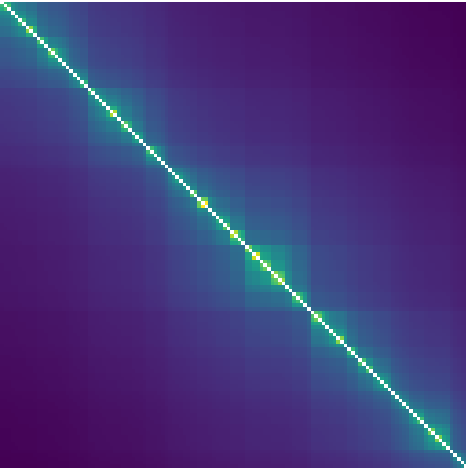
\includegraphics[height=0.4\textheight]{figures/dense_1d}

      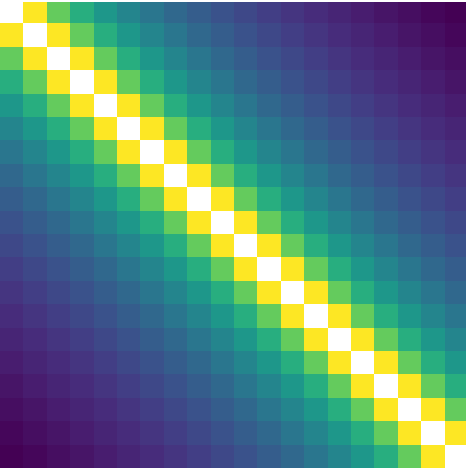
\includegraphics[height=0.4\textheight]{figures/grid_1d}
    \end{center}
  \end{columns}
\end{frame}

\begin{frame}{Layered redundancies}
  \begin{center}
    Algorithmic complexity: $\displaystyle\mathcal{O}(N_t N_s^2)$
  \end{center}
  \begin{block}{Rotating-wave approximation}
    High-frequency terms barely affect dynamics; formulate equations without them.
  \end{block}
  \begin{block}{Fewer degrees-of-freedom}
    $g(\vb{r}, \vb{r}')$ has the same value at large distances; aggregate sources and transmit once.
  \end{block}
  \begin{block}{Imposed translational invariance}
    $g(\vb{r}, \vb{r}') = \vb{g}(\abs{\vb{r} - \vb{r}'})$ redundant on grid; employ FFT to accelerate $\int_{}g(\vb{r} - \vb{r}') \vb{J}(\vb{r'}) \dd[3]{\vb{r}'}$.
  \end{block}
  \begin{center}
    Optimal algorithmic complexity: $\displaystyle\mathcal{O}\qty(\frac{N_t}{\alpha} N_s \log N_s)$
  \end{center}
\end{frame}

\begin{frame}{Collective dynamics}
  \vspace{0.5cm}
  \begin{center}
    \begin{filecontents}{high_density_stats.dat}
time     ubound               lbound              p1                 p2                 p3                 p4                  p5                 p6                 p7                 p8                  p9                 p10                p11                p12                p13                p14                p15                 p16                 p17                 p18                p19                 p20                 p21                 p22                p23                 p24                 p25                p26                 p27                p28                 p29                p30                p31                p32                 p33                p34                p35                 p36                 p37                p38                p39                p40                 p41                p42                p43                p44
0.       1.                   1.                  1.                 1.                 1.                 1.                  1.                 1.                 1.                 1.                  1.                 1.                 1.                 1.                 1.                 1.                 1.                  1.                  1.                  1.                 1.                  1.                  1.                  1.                 1.                  1.                  1.                 1.                  1.                 1.                  1.                 1.                 1.                 1.                  1.                 1.                 1.                  1.                  1.                 1.                 1.                 1.                  1.                 1.                 1.                 1.
0.15625  0.9999999999996378   0.999999999999718   0.9999999999997039 0.9999999999997039 0.9999999999997039 0.9999999999997039  0.9999999999997039 1.                 0.9999999999997    0.9999999999997039  0.9999999999997039 0.9999999999997039 0.9999999999998039 0.9999999999997039 0.9999999999997039 0.9999999999997039 0.9999999999996766  0.9999999999996766  0.9999999999997039  0.9999999999997039 0.9999999999995945  0.9999999999996766  0.9999999999997039  0.9999999999997039 0.9999999999996766  0.9999999999997039  0.9999999999997039 0.9999999999996766  0.9999999999997039 0.9999999999997039  0.9999999999998    0.9999999999997039 0.9999999999997039 0.9999999999996766  0.9999999999997039 0.9999999999997039 0.9999999999997039  0.9999999999996766  0.9999999999997039 0.9999999999997039 0.9999999999997039 0.9999999999996766  0.9999999999997039 0.9999999999997039 0.9999999999997039 0.9999999999996766
0.3125   0.9999999999967255   0.9999999999972855  0.9999999999971938 0.9999999999970001 0.9999999999971    0.9999999999970001  0.9999999999973063 0.9999999999999    0.9999999999983    0.9999999999970001  0.9999999999971    0.9999999999972    0.9999999999993062 0.9999999999975437 0.9999999999971062 0.99999999999735   0.9999999999970001  0.9999999999968     0.9999999999969937  0.9999999999971501 0.9999999999959562  0.99999999999695    0.9999999999970001  0.9999999999972062 0.9999999999968999  0.9999999999970499  0.9999999999969937 0.9999999999968999  0.99999999999735   0.9999999999970001  0.9999999999992    0.9999999999971062 0.9999999999970938 0.9999999999970001  0.9999999999971501 0.9999999999971    0.9999999999969937  0.9999999999970001  0.9999999999975437 0.9999999999970938 0.9999999999975563 0.9999999999968999  0.9999999999972    0.9999999999970938 0.9999999999973    0.9999999999970001
0.46875  0.9999999999808656   0.9999999999843944  0.999999999985175  0.9999999999831289 0.9999999999839    0.9999999999831289  0.999999999985875  0.9999999999995    0.9999999999940515 0.999999999982829   0.9999999999839    0.999999999985275  0.999999999998025  0.999999999988825  0.9999999999836234 0.9999999999868555 0.999999999982829   0.999999999981232   0.9999999999830289  0.9999999999844039 0.9999999999758055  0.9999999999822304  0.9999999999832055  0.9999999999848984 0.9999999999821524  0.9999999999833289  0.9999999999834055 0.9999999999822304  0.9999999999867555 0.999999999982925   0.9999999999978288 0.9999999999836054 0.9999999999843765 0.9999999999828251  0.9999999999844039 0.9999999999839    0.9999999999833055  0.9999999999828251  0.999999999988625  0.9999999999840999 0.9999999999885523 0.999999999982225   0.999999999985275  0.9999999999842094 0.9999999999860789 0.9999999999830289
0.625    0.999999999908596    0.9999999999258837  0.9999999999343    0.9999999999218    0.9999999999261    0.9999999999207     0.9999999999398    0.9999999999982    0.9999999999745    0.9999999999185     0.9999999999262    0.9999999999359    0.9999999999896    0.999999999957     0.9999999999246    0.9999999999455    0.9999999999187     0.9999999999081     0.9999999999199     0.9999999999296    0.9999999998857     0.9999999999145     0.9999999999211     0.9999999999334    0.9999999999144     0.9999999999222     0.999999999923     0.9999999999146     0.999999999945     0.9999999999198     0.9999999999912    0.999999999924     0.99999999993      0.9999999999193     0.9999999999295    0.9999999999261    0.9999999999221     0.9999999999193     0.9999999999558    0.9999999999277    0.9999999999555    0.999999999915      0.999999999936     0.9999999999278    0.9999999999406    0.9999999999203
0.78125  0.9999999996062331   0.999999999682793   0.9999999997345218 0.9999999996728851 0.9999999996924008 0.9999999996631351  0.9999999997641874 0.9999999999937249 0.9999999998902883 0.9999999996511656  0.9999999996931024 0.9999999997453626 0.9999999999614344 0.9999999998413492 0.9999999996856117 0.9999999997915087 0.9999999996531141  0.9999999995976     0.9999999996584656  0.9999999997118507 0.9999999995090422  0.999999999629818   0.9999999996664891  0.9999999997320203 0.9999999996306156  0.9999999996715313  0.9999999996776078 0.9999999996309157  0.9999999997894055 0.9999999996594852  0.9999999999619024 0.9999999996819797 0.9999999997163258 0.9999999996570602  0.9999999997114507 0.9999999996925008 0.9999999996720367  0.9999999996575836  0.9999999998366266 0.9999999997014297 0.9999999998353032 0.9999999996334461  0.9999999997456719 0.9999999997021313 0.9999999997681414 0.9999999996624351
0.9375   0.999999998423238    0.9999999987352037  0.9999999989906563 0.9999999987220313 0.9999999988035625 0.999999998665      0.9999999991224375 0.999999999978     0.9999999995845312 0.9999999986101625  0.9999999988072125 0.9999999990438062 0.999999999864825  0.9999999994213188 0.9999999987745625 0.9999999992340001 0.9999999986208062  0.9999999983684813  0.9999999986432062  0.9999999988942937 0.9999999980236     0.9999999985111375  0.9999999986848437  0.9999999989852687 0.9999999985182437  0.9999999987070437  0.999999998739225  0.9999999985183375  0.9999999992258625 0.9999999986532     0.9999999998615687 0.999999998757325  0.9999999989193376 0.9999999986427562  0.9999999988926938 0.9999999988045125 0.9999999987114875  0.9999999986464     0.9999999994049688 0.9999999988461062 0.999999999399775  0.9999999985303375  0.99999999904465   0.99999999884905   0.999999999138075  0.9999999986671437
1.09375  0.9999999940489793   0.9999999952373225  0.9999999963479899 0.9999999952728461 0.9999999955910476 0.9999999950002493  0.999999996861832  0.9999999999240594 0.9999999985257406 0.9999999947739383  0.9999999956068907 0.9999999965637523 0.9999999995107961 0.999999997934232  0.9999999954773625 0.9999999972779687 0.9999999948234539  0.9999999937785585  0.999999994911714   0.9999999959677766 0.9999999925190461  0.9999999943572149  0.9999999950989266  0.9999999963351898 0.9999999943956344  0.9999999951888188  0.9999999953337406 0.9999999943929788  0.9999999972475742 0.9999999949677757  0.9999999995313711 0.9999999954028297 0.9999999960787039 0.9999999949264117  0.9999999959613516 0.9999999955957977 0.9999999952134094  0.9999999949448812  0.9999999978805375 0.9999999957691601 0.9999999978612594 0.9999999944445     0.999999996567204  0.9999999957811352 0.9999999969209227 0.9999999950272148
1.25     0.9999999786802626   0.9999999829748861  0.9999999873838    0.9999999833523    0.9999999845301    0.9999999822076     0.9999999892247    0.999999999747     0.9999999949316    0.999999981339      0.999999984591     0.9999999881671    0.9999999983789    0.999999992916     0.9999999841106    0.9999999906873    0.999999981548      0.9999999775189     0.9999999818755     0.999999985967     0.9999999731747     0.9999999797126     0.9999999826382     0.9999999873396    0.999999979885      0.9999999829849     0.999999983565     0.9999999798681     0.9999999905796    0.9999999821315     0.9999999984377    0.9999999838146    0.9999999863999    0.9999999819772     0.9999999859431    0.9999999845483    0.9999999830925     0.9999999820592     0.9999999927398    0.9999999852132    0.9999999926722    0.9999999800699     0.9999999881793    0.9999999852584    0.9999999894365    0.9999999823664
1.40625  0.9999999272801493   0.9999999420531726  0.9999999583800921 0.9999999440757765 0.9999999482292625 0.9999999396845961  0.9999999645885219 0.9999999991969437 0.9999999833515648 0.9999999365395383  0.9999999484414039 0.9999999610146008 0.9999999948925906 0.9999999768946609 0.9999999467628617 0.9999999695068227 0.9999999373624227  0.9999999227155422  0.9999999385123649  0.9999999533561945 0.9999999083548656  0.9999999305766102  0.9999999413922899  0.9999999581800172 0.9999999312669758  0.9999999426746101  0.9999999448047523 0.9999999311941125  0.9999999691427407 0.9999999395456657  0.9999999950124602 0.999999945659132  0.9999999549106234 0.9999999390013922  0.9999999532718813 0.9999999482873766 0.9999999430834844  0.999999939334011   0.9999999763189898 0.9999999506743242 0.9999999760925391 0.999999931930725   0.9999999610560695 0.999999950835007  0.9999999653116531 0.9999999404196835
1.5625   0.9999997634759841   0.9999998119244535  0.9999998689657188 0.9999998207125438 0.9999998346763562 0.9999998050000437  0.9999998889140375 0.999999997580625  0.9999999481302437 0.9999997941730124  0.9999998353618937 0.9999998773388    0.9999999844830187 0.9999999284762    0.9999998298017875 0.9999999047928312 0.9999997972325875  0.99999974670155    0.9999998010659312  0.9999998519766813 0.9999997013328125  0.999999773481125   0.9999998112777063  0.9999998680630124 0.9999997760322625  0.9999998158279187  0.9999998231252875 0.9999997757701999  0.9999999036197187 0.999999804888725   0.999999984990125  0.999999825908525  0.9999998572278562 0.9999998030604937  0.9999998516934812 0.9999998348345438 0.9999998172321375  0.9999998043226312  0.9999999266520312 0.9999998429381125 0.9999999259311437 0.99999977830205    0.9999998774733813 0.9999998434819063 0.9999998912685    0.9999998079674938
1.71875  0.9999992657481732   0.9999994174512327  0.9999996065449336 0.9999994514443328 0.9999994962034805 0.9999993983788297  0.9999996678671633 0.9999999930746586 0.9999998459338445 0.9999993628208742  0.9999994982865539 0.9999996319167062 0.9999999554066086 0.9999997896366117 0.9999994807545695 0.9999997169954757 0.9999993736108758  0.9999992075762125  0.9999993857780687  0.9999995517237132 0.9999990713779602  0.9999992945577485  0.9999994200338539  0.9999996028288617 0.9999993033950507  0.9999994355147562  0.999999459068825  0.9999993025543196  0.9999997133964711 0.999999398982075   0.9999999570560243 0.9999994677135234 0.9999995685945571 0.999999393109743   0.9999995508170203 0.9999994965676352 0.9999994399548563  0.9999993976388547  0.9999997841455351 0.9999995227209023 0.9999997819652711 0.9999993108050593  0.9999996323329914 0.9999995244753351 0.9999996751732155 0.9999994092829789
1.875    0.9999978233778156   0.9999982770413197  0.9999988738026    0.9999983982857    0.999998535068     0.9999982280059     0.9999990541758    0.9999999811351    0.9999995625785    0.9999981164355     0.9999985410672    0.9999989472875    0.999999878003     0.9999994113166    0.9999984883253    0.9999991994019    0.9999981526095     0.9999976319912     0.9999981894575     0.9999987049912    0.9999972435867     0.9999979017648     0.9999982986505     0.9999988598901    0.999997930696      0.9999983490993     0.9999984211316    0.999997928221      0.9999991888973    0.9999982324651     0.9999998826198    0.9999984467653    0.9999987567554    0.9999982143835     0.9999987022235    0.9999985357246    0.9999983621354     0.9999982298375     0.9999993957231    0.9999986161859    0.999999389454     0.999997953812      0.9999989485135    0.9999986215845    0.9999990757678    0.9999982652555
2.03125  0.999993836122056    0.9999951322172571  0.9999969282002235 0.9999955370652742 0.9999959356040649 0.9999950159765015  0.9999974351365031 0.9999999510493156 0.9999988142950055 0.999994681347136   0.9999959520425946 0.9999971314968742 0.9999996814030625 0.9999984313948961 0.9999958004869187 0.999997844361943  0.9999947967673016  0.9999932372244649  0.9999949034195305  0.9999964321703532 0.9999921843616578  0.9999940367740844  0.9999952350187461  0.9999968802203101 0.9999941266736969  0.9999953923837586  0.9999956017241289 0.9999941199092922  0.9999978151984492 0.9999950362631336  0.9999996943350171 0.9999956743551867 0.999996584011818  0.9999949828042212  0.9999964241123344 0.9999959361996297 0.9999954280013149  0.9999950330895672  0.9999983895668235 0.9999961724840414 0.9999983724203062 0.9999941956101766  0.9999971349335031 0.9999961883364539 0.9999974958872687 0.9999951356743446
2.1875   0.9999833196842388   0.9999868588532511  0.9999920177186813 0.9999881336051625 0.9999892408436063 0.9999866096947563  0.9999933768817563 0.9999998789777063 0.9999969324332687 0.9999856501841937  0.9999892838023188 0.9999925539548937 0.9999992088165375 0.9999960196330687 0.9999888675262063 0.9999944747355    0.9999860009937626  0.999981534978      0.9999862963893374  0.9999906269787563 0.9999788252121375  0.9999838003529687  0.99998725728185    0.999991863540975  0.9999840661449563  0.9999877269975626  0.9999883060202562 0.9999840489128813  0.9999943977309188 0.9999866867971188  0.9999992429329875 0.9999885027824125 0.9999910526761188 0.9999865348807813  0.9999906046044625 0.9999892389675438 0.9999878173123374  0.9999866911468375  0.9999959132677563 0.999989901650175  0.999995868652275  0.9999842627100249  0.999992563119625  0.9999899460782188 0.9999935395678875 0.9999869740320124
2.34375  0.9999568514123776   0.9999660913953254  0.9999802421425906 0.9999698919570587 0.9999728253504883 0.9999656279495711  0.9999837141491063 0.9999997149504485 0.999992418355907  0.9999629975198234  0.9999729325958203 0.9999815881115257 0.9999981291529391 0.9999903830588086 0.9999718392366618 0.9999865168556579 0.9999640140467774  0.9999517824757235  0.9999647977305609  0.9999765216745492 0.9999451716970601  0.9999579199941743  0.9999674572705914  0.9999797768993836 0.9999586687457117  0.9999687988595727  0.9999703240285359 0.9999586279014164  0.9999863234989742 0.9999658915270071  0.9999982146260962 0.9999708339118915 0.9999776616533477 0.9999654763145868  0.9999764624314117 0.9999728114953789 0.9999690095861031  0.9999659404914563  0.9999901259823117 0.9999745868099766 0.9999900155532719 0.9999592046835539  0.9999816113551899 0.9999747056508039 0.9999841287235867 0.9999666828648351
2.5      0.99989327285144     0.9999163456204234  0.9999534236042    0.9999271013106    0.9999345119918    0.9999156780111     0.9999618668278    0.9999993604987    0.9999820872743    0.9999087833682     0.9999347680688    0.9999566331453    0.9999957847582    0.9999778811905    0.9999320212829    0.9999686747521    0.9999115936459     0.9998795433882     0.9999135867683     0.9999439276522    0.9998642760212     0.9998954466414     0.9999206221391     0.9999520989158    0.9998974582692     0.9999242892637     0.9999281152848    0.9998973688401     0.9999682131372    0.9999165117873     0.9999959882605    0.9999293796833    0.9999468419839    0.9999154198574     0.9999437780879    0.9999344558685    0.9999247334799     0.9999167385462     0.999977290235     0.9999389990407    0.9999770303036    0.9998988555312     0.9999566891882    0.9999393024278    0.9999628719438    0.9999185913083
2.65625  0.9997474958273399   0.9998026215271193  0.9998954455915078 0.9998315627221531 0.9998494138223282 0.9998022487263516  0.9999149807482837 0.9999986335938688 0.9999595346875992 0.9997849691981445  0.9998499993517562 0.9999027065464945 0.9999909589751469 0.9999515791269937 0.9998433978765289 0.9999307153608188 0.999792386928468   0.9997120171900445  0.9997972496513625  0.9998723234367383 0.9996786953456765  0.9997514347131546  0.9998150450373399  0.9998918769317063 0.9997565924852485  0.9998246402553875  0.999833778461339  0.9997564143411805  0.9999296678820336 0.9998047218410819  0.9999914138620898 0.9998367799939485 0.9998794333234445 0.9998019581973298  0.9998719634961781 0.9998492312085343 0.9998254524410977  0.9998055426630765  0.9999502880374945 0.9998603370210195 0.999949706344857  0.9997600757015382  0.9999028349503226 0.9998610761220632 0.999917298550007  0.9998099355879118
2.8125   0.9994284016354907   0.9995544669536695  0.9997765371243563 0.99962860085015   0.9996695931870188 0.9995565230282375  0.9998195260778563 0.9999972194627937 0.9999125630175563 0.9995151114735     0.9996708774877126 0.9997921046384313 0.9999815335308437 0.9998991169886124 0.9996556973671376 0.9998541269374562 0.9995338170496187  0.9993408996497251  0.9995452044595875  0.9997228340848938 0.9992723576266125  0.999434367015975   0.9995882575481     0.9997674284852938 0.9994469943428937  0.9996122963787688  0.9996330659676688 0.999446681534675   0.999851868653275  0.9995634495210874  0.9999824985124125 0.99963988946125   0.9997393830928437 0.9995567169189751  0.9997220085541001 0.9996690740027563 0.9996134427939251  0.9995660425723125  0.999896439772875  0.9996950057714813 0.999895202484275  0.9994552962530562  0.9997923840455125 0.9996967237376188 0.9998246080840438 0.9995759228720688
2.96875  0.9987615204287901   0.9990375720910627  0.9995453355393976 0.9992185137361164 0.9993082203271335 0.9990486654513445  0.999635294157225  0.9999946110174477 0.9998191823654969 0.9989537558398665  0.9993109297347937 0.9995769415029875 0.9999640729844664 0.9997999645080992 0.9992775264552469 0.9997076800946164 0.9989988476789571  0.9985554949643789  0.9990244553777523  0.9994263922532125 0.9984231479900915  0.9987675420856484  0.9991241040508648  0.9995232980690243 0.9987970735157976  0.9991817782162484  0.9992266662857906 0.9987966260118555  0.9997030567415695 0.9990670553964703  0.9999660083885734 0.9992415267425219 0.9994631391882179 0.9990512684368914  0.9994245884583187 0.9993068900098507 0.999182374743029   0.9990744970802219  0.9997947024721453 0.9993647237183657 0.9997922017498164 0.9988159875450148  0.9995775185297938 0.9993685328539345 0.9996458843522469 0.9990955306120055
3.125    0.9974307479822859   0.9980097825867267  0.9991194736756    0.9984308668207    0.9986178534021    0.9980472491392     0.9992984772852    0.9999900519254    0.9996419842256    0.9978392298198     0.9986233725839    0.9991802142486    0.9999334405197    0.9996225177909    0.9985530258935    0.9994425116943    0.9979431832976     0.9969675953397     0.9979985003279     0.9988683548261    0.9967290942772     0.9974278506835     0.9982191782227     0.9990689473422    0.9974938482377     0.9983516971898     0.99844386626      0.9974934702218     0.9994335291079    0.9980936448904     0.9999370546084    0.9984748812361    0.9989461943084    0.9980580185746     0.9988646016806    0.998614742494     0.9983480811711     0.9981134206419     0.9996127251785    0.9987379294357    0.9996079243346    0.9975350248194     0.9991813442168    0.9987459831015    0.9993194396793    0.9981556647518
3.28125  0.9948952218106036   0.9960590459440165  0.9983769719683788 0.9969937833474102 0.9973647616264383 0.9961633567557118  0.9987157576455039 0.9999825077848836 0.9993211789261508 0.9957273811583351  0.9973756790063578 0.9984875248359211 0.9998825611981211 0.9993220704202211 0.9972338698346047 0.9989882805710211 0.995956620980039   0.9939012300273242  0.9960714235978476  0.9978718972172422 0.9935036971235078  0.9948568413160938  0.9965390097660398  0.998267300216368  0.9949978116245008  0.9968305647335359  0.997010193920007  0.9949982902276133  0.998971732274682  0.996274737634179   0.9998887780103657 0.9970722474039735 0.9980291981696562 0.9961973867705797  0.9978644653848554 0.9973581042711313 0.9968116097501007  0.9963239118807093  0.9993048291028477 0.9976086797652968 0.9992960793037937 0.9950834258874086  0.998489620610579  0.99762490959465   0.9987551428055321 0.9964035637096179
3.4375   0.9902835839586688   0.9925256827194247  0.997152505779175  0.9945052259033187 0.9952050754577125 0.992782648489575   0.9977628510276312 0.9999707023256376 0.9987676063501062 0.9919091185377875  0.995226207498775  0.997343523670975  0.9998026347900375 0.9988413007903063 0.9949525215667624 0.9982530041730625 0.9923926431731562  0.9882478628922     0.9926215159845124  0.9961856049124875 0.9876442182723687  0.990144980740875   0.9935692913151251  0.9969275553342438 0.990432770710075   0.9941831609219     0.9945151730965375 0.9904362346979687  0.9982241283327937 0.9930372450592813  0.9998122189501    0.9946342261148937 0.996488914479575  0.9928757563403624  0.9961716108714562 0.9951921139685063 0.9941202127964125  0.9931523586691875  0.9988125975571625 0.9956787982926313 0.9987974704544875 0.9906026517433125  0.9973471995824312 0.9957099523659437 0.9978330228233813 0.9932922724331625
3.59375  0.9822801965724725   0.986420801839751   0.9952435875513117 0.9904196328911805 0.9916733015723406 0.9869971298026617  0.996292092351414  0.9999532585198586 0.997859051944264  0.9853246649025594  0.9917137071043992 0.9955588037881079 0.9996841072402305 0.9981152347699149 0.991207873683239  0.9971298632945008 0.986299714472964   0.9783048484525868  0.9867378053329883  0.9934840543591883 0.9774929789921297  0.9819032015883492  0.9885748938069492  0.994808896709464  0.9824645321432227  0.9898106039154696  0.9903924675645821 0.9824757418383758  0.9970822114109867 0.9875512069833648  0.9996963698840242 0.9906115446519492 0.9940422902964438 0.987227292736171   0.99345902282155   0.9916507618811399 0.9896382818379711  0.9878057850000305  0.9980700614644719 0.9925532386873187 0.9980452849747672 0.9827859221849571  0.995564888246736  0.9926101556192758 0.9964104942996641 0.9880318536300765
3.75     0.9690371819208891   0.9763668185033579  0.9924301262423    0.984068867576     0.9861972971331    0.9775600414971     0.994153371639     0.9999289701699    0.9964464138618    0.9745021780701     0.9862743605383    0.992933098629     0.9995184605489    0.9970822414384    0.9853786553122    0.9955138185426    0.9763802979915     0.9616448322917     0.9771845901621     0.9893920152761    0.9607367511689     0.9681579269184     0.9805877569907     0.9916424740071    0.9692031114305     0.9829623103948     0.983930396813     0.9692313108032     0.9954396145124    0.9787071644778     0.9995282708465    0.9843171384568    0.9903733532825    0.9780837107097     0.9893495385385    0.9861638897292    0.9825463517035     0.9792400075415     0.9970150069573    0.9877615247761    0.996976637771     0.9697822199924     0.9929425749196    0.9878603914966    0.9943422180427    0.9795683515453
3.90625  0.9481695998830573   0.9606022034036836  0.9885051554731336 0.9747370855459617 0.9781527186186961 0.9628994251946164  0.9912300371540165 0.9998971925730672 0.9943798430805258 0.9575646699017328  0.9783004023780476 0.9892978572006038 0.9993009016143038 0.9957011898660282 0.9767796639464242 0.9933286974079679 0.9610154785581828  0.935104058731568   0.9624293436077133  0.9835406975545038 0.9344193376132741  0.9463347703020577  0.9684498175336187  0.987176600747418  0.9481897899191977  0.9727966330031461  0.974332080947328  0.9482509680237601  0.9932200193945329 0.9651551642930133  0.9992927922737461 0.9749871632077867 0.9851903379879149 0.964005448515946   0.9834724331664141 0.9781163668134094 0.971888139538271   0.9662113059816352  0.9956064043706985 0.9808167092419054 0.9955503993146125 0.9491828299310945  0.9893116842737141 0.9809797911718438 0.9915139728586305 0.9666194146556336
4.0625   0.9169092662695217   0.9371032415685216  0.9833051121377    0.9618002502182125 0.9669609093687437 0.9412323229627938  0.9874861129761062 0.9998582850894062 0.9915665269415125 0.9323588663528313  0.9672457922426188 0.9845750807314813 0.9990335435191    0.9939725183338375 0.9647671748354187 0.9905615171780126 0.9383965312581     0.895013957437325   0.9407704980033501  0.9756563050214    0.8951650887223125  0.9134218368771875  0.9509328036618813  0.9812436067115188 0.9165527847819313  0.958493649815925   0.9608365296332937 0.9166723105609688  0.9904125718672749 0.9454358883104312  0.9989717017149126 0.9619014940960875 0.97831276447945   0.9434081896115125  0.9755526336143625 0.9669552576900875 0.956678249918575   0.947417900994325   0.9938454948070187 0.971314833522925  0.993768816002375  0.9181730403708188  0.9845938549512687 0.97156991543255   0.9878868819815625 0.9477934708298625
4.21875  0.8724877138100092   0.9038679240435162  0.976718891722082  0.9449210261770922 0.9522169701995242 0.9108129864824835  0.983014677182007  0.999813980432968  0.9880658042425461 0.8967497751605007  0.9527673021047688 0.9788410496885758 0.9987279892604805 0.9919582635936071 0.9488819035819406 0.9872962663797531 0.9067897484018125  0.8378006028452468  0.9105845115994476  0.9656678141572625 0.8397049037289976  0.8664037381441726  0.9269377770136883  0.9738373098343727 0.8714127954912858  0.9393978466928601  0.9428924703870015 0.871629497451003   0.9871067550171085 0.9182154296770234  0.9985422461135195 0.9445548462483712 0.9697758003203288 0.9148017051057944  0.9655194712319485 0.9523334859841125 0.9360643118320258  0.9217350878970163  0.9917953981901187 0.9590624337066781 0.9916976502956195 0.8739309775972702  0.9788645052040351 0.9594401206418062 0.9835423255421882 0.9218019695498118
4.375    0.8127680453304472   0.8593673366792     0.9686532829154    0.9242634857953    0.9338152982288    0.8703156536076     0.9780722218864    0.9997675224897    0.9842049362889    0.8490824020959     0.9348688355816    0.9723765399683    0.9984064780323    0.9897940817376    0.9289960153986    0.9837360497555    0.8649207040058     0.7609958717562     0.8706720878323     0.9538071521805    0.7657368582201     0.8030011580544     0.8957448247158     0.9651813097789    0.8105653114936     0.9151407728288     0.9203499138338    0.8109402956027     0.9835150749574    0.8825966854758     0.9979770479668    0.9228433765829    0.9599259355907    0.8771197111013     0.9536079824174    0.9342575236203    0.9095114725588     0.8885078312445     0.9895923470429    0.9442022200404    0.9894776501609    0.8143037412942     0.9724029566269    0.9447304946101    0.9787135917432    0.8877403201307
4.53125  0.7370373467872192   0.8030945575455232  0.9589447355208001 0.900670258625186  0.9120295929002664 0.8192935237027681  0.9730830467022547 0.9997234350333398 0.9806561293739297 0.7887365412411149  0.9140035185207281 0.965683105527318  0.9981005494043094 0.9876860042908828 0.9054165294624735 0.9802022242529711 0.8124046181978243  0.6645160841491963  0.8206307281375149  0.9406682201661328 0.673027869074943   0.7226184114758821  0.8572490417602477  0.9557650844956906 0.7333465330653126  0.8856849633073508  0.8936127453140906 0.7339808619331704  0.9799713838076586 0.8384332169906453  0.9972496288694914 0.8972108322765008 0.9494736415366204 0.8300687107406283  0.9404188481904734 0.9131927900182671 0.8769569342828009  0.8478216762890142  0.9874418125093921 0.9272967604436375 0.9873201811547867 0.7386705639152619  0.9657087965885469 0.9279928638502235 0.9737904004256859 0.845372582929272
4.6875   0.6467307930663603   0.7360520403512382  0.9472334225809    0.8757377577778188 0.8875133778817563 0.7585860663238625  0.9686024180794187 0.99968687292155   0.9783703557417875 0.716616614132625   0.8910925676308937 0.9594499637753562 0.9978464317435938 0.9858868546923563 0.8789027576929312 0.9771027247531    0.7500944126848562  0.5518137980432187  0.7611402748005938  0.9271970767964812 0.5644878981822937  0.6272205906285125  0.8121026979740563  0.9463302672622    0.641434117329125   0.8512574764216251  0.8636939875030062 0.64249282366305    0.9768962544343187 0.7865406710254187  0.9963529167418    0.8686975647866501 0.93947023786125   0.7743851032730813  0.9269087846572187 0.8900844900249563 0.8388818291392125  0.8006534656862937  0.9855953127572687 0.9093348973282688 0.9854824288666625 0.6487390575059188  0.9594691295385    0.9101955979796063 0.9692875898975937 0.7953284250280188
4.84375  0.54576297043116     0.6609670019073741  0.9328466290437203 0.8517352965476148 0.8612150582985523 0.6905043940700655  0.965236395182082  0.9996626509988726 0.9782706079367665 0.6353760101532498  0.8674440063453375 0.9544668455336422 0.9976781821208539 0.9846522025123867 0.8505822573650343 0.9748687487677695 0.6802027401666256  0.43034190709125764 0.6940493328706311  0.9146032759839883 0.44678094040103106 0.5217321473866647  0.7617011124010179  0.9378023456904125 0.539231197300599   0.8121974329241296  0.8321404848586663 0.5409523259739014  0.9747284441823336 0.7287125768933077  0.9953371719946782 0.8388609835425429 0.931189164082807  0.7118926704520601  0.9143008499870765 0.8662756834394656 0.7962718209192476  0.7488290582860366  0.984308370018093  0.8916463279076469 0.9842227166443976 0.5489048108613327  0.9544721480306735 0.8926386735733288 0.9657776248381726 0.739129575467732
5.       0.440192708281556    0.5820672077793234  0.9147643899926    0.8313354969085    0.8342346196454    0.6186550409647     0.9635277955729    0.9996541934296    0.9807425746168    0.5492222833457     0.8445876194043    0.9514916300527    0.9976201908094    0.98418308007      0.8217863887008    0.9738681275918    0.6061042833276     0.3108672374927     0.6222046970617     0.9042043326617    0.3299633797359     0.4136051333955     0.7079993621934     0.9311780188922    0.4335394372088     0.7687932309341     0.8008365652778    0.4361838800481     0.973832152699     0.6675077030767     0.9943559498445    0.8095775814992    0.9259140421258    0.6453093119265     0.9039262802178    0.8433382022175    0.7504756902986     0.6947818269307     0.983786236278     0.8757375172342    0.9837435471979    0.4458599734675     0.951475770652     0.8767928819498    0.9637950652727    0.679012572005
5.15625  0.3371862296852923   0.5044013132783025  0.8917554932936594 0.8171504327335672 0.8076690500879422 0.5473836827413087  0.9638298708333626 0.9996627242089782 0.9852233542551524 0.46329005516780636 0.8240685776895805 0.9510945254299906 0.9976810496614492 0.9845707015334187 0.7938542706458329 0.9743134763324953 0.5318322805305806  0.20558836458395327 0.5490522602353244  0.8972320689706094 0.22577987824886808 0.3115062761397439  0.6532065377400477  0.9273885223861312 0.3324776180976627  0.7211962599047579  0.7717360759797142 0.3361734909498111  0.974401466627318  0.605860386845397   0.9936674134347789 0.7827740406475289 0.9246631900205695 0.5778421773949282  0.8970266217179781 0.8228588918682953 0.7030038974188055  0.6411801701269438  0.9841304353353977 0.8630839971848758 0.9841372749382586 0.3474142069235837  0.9510527780832188 0.8640984032585657 0.9637277860516703 0.617586222386036
5.3125   0.24357315452278194  0.43288647297496874 0.862765982355525  0.8111023734340937 0.7824914650482625 0.4809867878602875  0.9661999304556688 0.9996869712205813 0.9903293544780938 0.382743416965775   0.8072491100752001 0.9535111588535687 0.9978514450877874 0.9857633694466312 0.7679601132301438 0.9761912150084625 0.46140240528939996 0.12556138014585    0.4781148594679062  0.8946355871273625 0.144767702779775   0.22349550461621248 0.5994451663576937  0.9271590077593188 0.24393749358663125 0.6694622415226438  0.746590003660775  0.24841579843175002 0.9763921874646749 0.5466305300478626  0.9935242983029563 0.7601505165681812 0.9279083474103188 0.5126893687960875  0.8945515043390688 0.8062314847057813 0.6553230507319749  0.5905349719320563  0.9853036299577438 0.8549213227467625 0.9853535700304062 0.26087415231689376 0.9534441906766687 0.8557646226149063 0.9657150130285438 0.5574216686429125
5.46875  0.16450733879275267  0.3713973853147986  0.8275778063084023 0.8137133747321875 0.759490165523621  0.422954576595371   0.9703503828908757 0.9997234855627859 0.9945963045959296 0.3118860202854835  0.7951552110544883 0.9585439214560696 0.9981066723896523 0.9875727079744219 0.745004238878696  0.9792398240193251 0.398166248631189   0.07828627911480192 0.41248581588762256 0.8969119771784492 0.09321332481522245 0.15535131729841944 0.5484683673830234  0.9308736836126993 0.17408676808849444 0.6137129579273867  0.7267267155479452 0.17838449142084914 0.9795111450713453 0.4922234032483679  0.993995057446786  0.7429491974593398 0.9353699461762719 0.4525938400835757  0.8969845529911571 0.7944927878915445 0.6086957848347875  0.5448903078282992  0.9871293166365539 0.852069506621693  0.9872048065228852 0.19157076119886945 0.9584595190332649 0.8526050795362039 0.9695776803234009 0.500691555964046
5.625    0.10269440972262335  0.322190723441115   0.7875815182558    0.8234921566845    0.7392708272429    0.3754945205591     0.9756873965545    0.9997674605465    0.9972302814491    0.2535487089527     0.7883837119662    0.965551232965     0.9984125174327    0.9897227019351    0.7255829181083    0.9829970323303    0.344377804169      0.06625070021032    0.3544581285068     0.9039890118017    0.071580663143      0.1096371267785     0.5014985198506     0.9384459720012    0.1263903840681     0.5543604413313     0.712913117728     0.128662771765      0.983278555003     0.4443680618464     0.9949057286612    0.7317962850987    0.945983442547     0.3995605555104     0.90422405215      0.7882206340828    0.5640961150024     0.5056538970909     0.989333136365     0.8548113264152    0.989412938632     0.1420487900225     0.9654633030845    0.8549261844321    0.9748110770053    0.4489466045637
5.78125  0.05836312082558641  0.2858001781697629  0.7462621365835118 0.8367062298960249 0.7223061788153945 0.3394476465932961  0.981441609820382  0.9998137743980383 0.9982441952252407 0.20889773197872974 0.7870669873812508 0.973551608958386  0.9987329290141461 0.991925013557114  0.710027621630225  0.9869129016874555 0.3010616380380743  0.08684249004674019 0.3053540463229524  0.9151809412375133 0.07529185500442506 0.08573532243770025 0.4592054891897188  0.9492030771793648 0.10136512855524846 0.49230899741974543 0.7052957715822273 0.09894369899799371 0.9871507253491352 0.4040726885768016  0.9959841558326585 0.7266227930813359 0.9581095206552    0.35477422011938836 0.9155426058344859 0.787492980888193  0.5222071017125266  0.4735661259679782  0.9916150604608609 0.8628337485915828 0.99168302806165   0.1120919709650055  0.9734757588912226 0.8624755426778101 0.9806657360260781 0.40306093498649537
5.9375   0.029831366787123337 0.2613402992657099  0.70891486501115   0.847826734376675  0.7090042548951188 0.3145372746507125  0.9868558672345813 0.9998579435216187 0.9981018521492375 0.17763559712223748 0.7908849654984438 0.9814367848948    0.9990368728528438 0.9939495213658437 0.6984866369744063 0.9904942950869    0.26815455820385625 0.13354934859455625 0.2655545661839125  0.9292401759461938 0.09708979117788624 0.08064968749967937 0.42179983774671875 0.96184105043495   0.09698463878691249 0.42905154504535    0.7034068351298812 0.08672829640310312 0.9906604512782126 0.37171191755613747 0.997023620036     0.7266617752743812 0.9699756579919437 0.31868105336220626 0.9296510482116125 0.7919000626323813 0.48348685420628124 0.4487648329857125  0.9937248078713438 0.8752400796771188 0.9937746259898    0.0993881485338875  0.9813840299207812 0.8744517875921687 0.986318285322175  0.3633205329233375
6.09375  0.014336520924414509 0.2470298091216951  0.681439802799682  0.8506912550117188 0.6997580691313976 0.2997781619182492  0.9913633882190899 0.9998967548312445 0.9973573227809195 0.1584411866044781  0.7991151110230758 0.9882394485739118 0.999302491170957  0.9956617629576633 0.6910126693438391 0.9934236878892172 0.24481173571749607 0.19793026319250168 0.2346772521501156  0.9445250613726078 0.1294399881492071  0.09013760189700175 0.38919080308205856 0.9745637171523187 0.10947204941600705 0.3666064933536257  0.7062245511240282 0.08833200867798384 0.9935201796591954 0.3471716135668265  0.9979123875946891 0.7305270447483954 0.9801922427488383 0.2911563278075602  0.9448854094072828 0.8006033417339656 0.448273301256657   0.4308910955236461  0.9955094106638945 0.8906451948566922 0.9955432100013634 0.10045474868474298 0.9882117395321829 0.8895815547476517 0.9910874797626382 0.32959464673430855
6.25     0.008814151742556703 0.24072984840966122 0.6686298539158    0.8400816999864    0.6949396251727    0.2938648555314     0.9946913640442    0.9999284889982    0.9964539107635    0.1494626705257     0.810715380538     0.9933609329847    0.9995184951021    0.9970190620315    0.6876193887377    0.9956026859712    0.2297504984817     0.2716001515733     0.2118267417028     0.9592817798028    0.1660762527101     0.1097523820434     0.3611539447278     0.9854975710649    0.1341951658812     0.3072959221745     0.7122922905388    0.0998230458207     0.995650397006     0.3299856561083     0.9985991903411    0.7363881057904    0.988079865151     0.271679945933      0.9595064533921    0.8124396884673    0.4168896672828     0.4191963121434     0.9969176141852    0.9073644927826    0.9969409438986    0.1114864481444     0.9933518026547    0.9062716159761    0.9946072275618    0.3015243397196
6.40625  0.010443232771723793 0.24035944107848792 0.6725974105244648 0.8132996396039985 0.6948157765587547 0.2954282498761914  0.9968620409669087 0.9999527835719187 0.9956337596581938 0.1487231956412203  0.8244383582419187 0.9966678383727414 0.9996830239808422 0.998040095991286  0.6882794368146664 0.9971105107870648 0.22153867244045314 0.34756857951194836 0.1958461498554758  0.9719906607498593 0.20262630713287652 0.13555567776604763 0.33746474239256646 0.9932995207943367 0.1664545241621648  0.25342705387191805 0.7199073514683008 0.11767405032421403 0.9971338143210625 0.31943265536836646 0.9990833407345515 0.742250140178418  0.9936237502361438 0.2594731054477305  0.972048151773982  0.8260694156465601 0.38971394096012657 0.41263816483131094 0.9979705482977461 0.9236851717013687 0.997987867223564  0.12894822479314372 0.9966677822853804 0.9228339149849961 0.9968728167887156 0.2786786046629024
6.5625   0.01692185366683263  0.24413968684255777 0.6917701903765374 0.7714115023514749 0.6993946027401124 0.30314425395900624 0.9981089739346876 0.9999702699465562 0.9949692451795126 0.154378936444475   0.8389728477319313 0.9984257158291813 0.9998008808144688 0.9987716988978375 0.6928572064607438 0.9981134986229749 0.218787315098475   0.4207077727217125  0.1855207353267875  0.9816747587314437 0.236545019279375   0.1644562285957625  0.3179741455672687  0.9976412687967313 0.2020531210812125  0.20697646402525    0.727378505688375  0.13908334265462502 0.9981302835721688 0.3145960926797187  0.9994045691094937 0.74631752590205   0.9971427452924375 0.2535872756922875  0.9816040094082875 0.8401572236856313 0.367188495021025   0.409974733717825   0.9987230684164875 0.9381666385222626 0.9987361442861438 0.1498912792500625  0.9984279814561625 0.9377544124584812 0.9981449817512688 0.26065352764023125
6.71875  0.026530118290683857 0.2506851508359294  0.7207620609471306 0.7197187337597296 0.7082503456505328 0.31574999969538675 0.9987527938556172 0.9999821379868422 0.9944711927522586 0.16483755749355392 0.8531002149912587 0.9991181047163954 0.9998805152559359 0.9992681800010641 0.7009982947418774 0.9987791801732788 0.22025161661667578 0.4875955950384798  0.17971443083436642 0.9880552444343305 0.26666584999994375 0.19425610562670395 0.30262287765482027 0.9992254684771821 0.23761866018299224 0.16936820479963824 0.7333206213880866 0.16203413607200395 0.9987978821200828 0.3144117987973086  0.9996107576648008 0.7473734597377758 0.998979476626721  0.25296278677699296 0.9879442985514079 0.8535571493766634 0.3497676360400211  0.40987104160879767 0.9992361986193165 0.9498804463755007 0.9992451213972656 0.1720542864869805  0.9991205425515797 0.9499444069863462 0.9987810193653687 0.24711308194676562
6.875    0.03806688150682956  0.2589915178676383  0.751488795545     0.6668256086393    0.7204047413743    0.3320447401322     0.9990846621426    0.9999897505759    0.9941426871965    0.1787805415302     0.8658408206877    0.9992453354969    0.9999314042384    0.9995835664586    0.7120240263584    0.9992296270882    0.2248662356867     0.5461527632196     0.1774431833188     0.991492979973     0.292713551142      0.2235257828147     0.2914080614294     0.9992861810947    0.2707063875702     0.1413893764375     0.7369208175344    0.1851970959235     0.9992504055185    0.3177264663091     0.999737270459     0.7450709359087    0.999440474893     0.2564806038596     0.9914286236115    0.8654576311703    0.3378231945181     0.411021590781      0.9995660536691    0.9585051530047    0.9995710027417    0.1938322463435     0.9992480437537    0.9588985800985    0.9990912471869    0.2377854267869
7.03125  0.05073560521785586  0.2683704072181013  0.7754548120560734 0.622243597964847  0.7343432342962867 0.35091936192523593 0.9992952959590344 0.9999943743453671 0.9939573080266859 0.19513682323452264 0.8765597286676031 0.999184575759157  0.9999622123836516 0.9997690768277648 0.724890550260182  0.9995360224008915 0.23174441993402028 0.5953293639804601  0.17790087741655    0.9927539566746687 0.3149525636868023  0.2514139965202656  0.28432521452901094 0.9989072544585968 0.2997433340185062  0.12323005347997971 0.7380950952695672 0.2077690517284453  0.999554406586775  0.3233761612251156  0.9998104716596828 0.7400286024141914 0.9989257975183313 0.26302154692977814 0.9927737454734132 0.875445823417975  0.33154168915335547 0.41227653437817346 0.9997626212901944 0.9642496742524593 0.9997646513732773 0.21418070222025232 0.9991868842760461 0.9647062319523461 0.9992754573504109 0.23243477228317425
7.1875   0.06402771535185689  0.27836944412927644 0.7862059600274313 0.5936487062967812 0.7482055911386937 0.3713981641221875  0.9994659627748063 0.9999970385606687 0.9938607489934626 0.21304194236681875 0.8850070002704375 0.9991421698017312 0.9999799149458938 0.9998699970205438 0.7382578317656062 0.999735955930975  0.24016257880296252 0.6348484323657625  0.1804553916693125  0.9927120474526188 0.33392725128566253 0.27746161221925625 0.28130956170918126 0.9986013979397874 0.32388393471185    0.11459869700436874 0.7374727454510187 0.22930925874868124 0.9997478990355625 0.3302764666327125  0.9998516182473876 0.7336735252519    0.9980040947467063 0.27153273216316876 0.9927895461025875 0.8834759707841687 0.33084583178420623 0.4127496409501875  0.9998698434924438 0.9676565621220625 0.9998703934103376 0.23249999470553123 0.99914225980945   0.9679162906352625 0.9994287386196062 0.23082747540441875
7.34375  0.07762642400336323  0.2886996561476542  0.7807988115056969 0.5851676078286414 0.7601217692855633 0.3926462123761125  0.9996079010908782 0.9999984977675641 0.9938194668853985 0.23180053807478362 0.8912851699301141 0.9991806948776906 0.9999895957992727 0.999921801459057  0.7506752659386547 0.9998536160720242 0.2495418927476711  0.6649405873596883  0.18462889354294923 0.9921082807480234 0.35024517714130937 0.3014528329302735  0.2821942216481617  0.9983546077549312 0.34283704957043676 0.11485917056606251 0.7361970833048531 0.24960413632403833 0.9998589459346985 0.3375060373468414  0.9998741969062734 0.7278601107275516 0.9972764645552687 0.28109079117864766 0.9921790774479898 0.8897625092600281 0.33536060279766955 0.41188810656070707 0.9999235904887523 0.9693808939190562 0.9999237172103554 0.24852444999606174 0.9991776556150805 0.9693128473047007 0.9995758107870937 0.2327050452899383
7.5      0.09133679607825397  0.2991791694059783  0.7601050861572    0.5969846120059    0.7685990325786    0.4139231245022     0.9997134249345    0.9999992593044    0.9938346095155    0.250857741475      0.89575722275      0.9992801755364    0.9999946456592    0.9999481697361    0.7608428258453    0.9999117377527    0.2594309289712     0.6860910344965     0.1900718195885     0.9914316915192    0.3644562924054     0.3233114479174     0.2866928906381     0.9979877978552    0.3567043496079     0.1231518345931     0.7355947901537    0.2685697173198     0.9999133146916    0.3443662258798     0.9998861721674    0.7243795707951    0.9971070068481    0.2909494378094     0.9914405921693    0.8946440706028    0.3444277295371     0.4094943347345     0.9999493236991    0.970026612434     0.9999494917101    0.2622276891777     0.9992755664221    0.9696838695235    0.9997053092951    0.2377695370134
7.65625  0.10503906365255891  0.3096939122841519  0.7284697221390305 0.6256875938132828 0.7728432004719649 0.43451387977893197 0.9997843695403968 0.9999996392365125 0.9939005416045609 0.26977828929199604 0.8989232272588414 0.9993961193403688 0.9999971682546758 0.9999622764955282 0.7678732978700961 0.9999333551054242 0.2694893872048859  0.6988790992887454  0.19653596625795156 0.9909191246665054 0.3770431943806125  0.34303589481733904 0.2944055886087797  0.997496863333139  0.3658492770275711  0.13848329508506715 0.7368116167088875 0.28618877278692967 0.9999336333897    0.35040767717391796 0.9998940691316547 0.7245099776403937 0.9974483868193829 0.3005635608433164  0.9908569281374391 0.8984667370241891 0.3571597652408328  0.40570131773352813 0.9999621101353758 0.9700711466983695 0.9999623898964063 0.2737468503836945  0.9993928888212492 0.969652047220718  0.9997975696866258 0.24568107424046873
7.8125   0.11865927897598125  0.3201721264946821  0.6929446576474313 0.6650215252575312 0.7729256488686688 0.45368892217815626 0.9998307112265062 0.9999998213012125 0.9939867081982687 0.2882300349426875  0.90129728532835   0.9994943667243812 0.9999983843315188 0.999970255245325  0.7714788139407438 0.999937646889825  0.27947214951525623 0.7039367377424313  0.20384937686866875 0.9906280165498125 0.38842984257615    0.36066228483206875 0.30484074837148123 0.9971149727620625 0.3708001702834688  0.15978627818149999 0.7405179962866875 0.30247453335921876 0.999937098309975  0.3554244332904125  0.999901270538275  0.728727690543925  0.9979301592542312 0.30958893674973753 0.9905353254583062 0.9015160351370188 0.37251917065670626 0.40091141526753127 0.9999692092002063 0.9698603609511562 0.9999694804223375 0.2833240934829625  0.999494120220575  0.9695995598279312 0.9998450302895188 0.2560641902552187
7.96875  0.1321515706735149   0.33056856219387576 0.661913814005985  0.7072040535225134 0.7697624878740406 0.4707242447062     0.9998586221677696 0.9999999057218836 0.9940733408965664 0.30596930813148676 0.9033098998465922 0.9995611301335945 0.9999989550957132 0.9999747173345664 0.7720308124187125 0.9999363244234336 0.2892132605394266  0.7019639532324023  0.21189433203282423 0.9905269458904593 0.39895057112626564 0.37624534567511486 0.31744580009722895 0.9971014607749156 0.37218224839934533 0.1859593208691016  0.746756870114168  0.3174523644667711  0.9999350381558468 0.3594227889423422  0.9999069047259961 0.7366349919416985 0.9981635891785703 0.317862182798657   0.9904648313763117 0.9040007642647132 0.38940749070883907 0.3957121169880633  0.9999734573149641 0.9696342333550336 0.9999735859236093 0.29126206317423753 0.9995626770139399 0.9696810373730554 0.9998590212757312 0.2685190906743852
8.125    0.14548759208578466  0.3408548363743984  0.6432305207099    0.7447302740226    0.7649208199712    0.4849681021946     0.9998684529547    0.9999999440502    0.9941706860741    0.3228271292923     0.9052498046841    0.9995978070455    0.9999992202109    0.9999769767976    0.7704797744959    0.9999343041693    0.2986101582313     0.6937203878722     0.220589182657      0.9905640300907    0.408835942468      0.3898499332216     0.3316399618423     0.9974860132629    0.3706699059386     0.2158969773716     0.7549587229793    0.3311523046581     0.9999335226661    0.3625746913417     0.9999107175752    0.7470961300336    0.9980331449181    0.3253681551446     0.9905724222468    0.9060718037938    0.4067520349946     0.3907829837308     0.9999758735123    0.9695500813018    0.9999758563208    0.2978899564536     0.999598563898     0.969894759281     0.9998598041754    0.282634784839
8.28125  0.15865019630174368  0.3510134902660321  0.6425088553351391 0.7720583318943688 0.7602983157212914 0.4959135290844149  0.9998631342478914 0.9999999614190765 0.994285994319657  0.3386961374746899  0.9072485762297984 0.9996120574608672 0.999999345641354  0.9999779393403242 0.7681545620366679 0.9999332238995289 0.30760886328051795 0.6799834025598054  0.22987428177002503 0.9906982032121648 0.4182571841442516  0.40154833872965706 0.3468452802559743  0.9980121909260031 0.3669512579457578  0.24851813004852197 0.76410547659505   0.34360746092057115 0.9999342507124211 0.36516491125312817 0.9999151659399274 0.7585319193979766 0.9977509714953008 0.33220196260969065 0.9907697425565883 0.9078517632943773 0.4235805195466891  0.3868066281512867  0.9999770430099297 0.9696909696487485 0.9999769661774344 0.30353760955755704 0.9996107996942828 0.9701734380793188 0.9998602447742515 0.2980022353197008
8.4375   0.17162952762586509  0.36103422436243043 0.6620473281640438 0.7866558742412187 0.7577421241551188 0.5032477005017187  0.9998526899771438 0.9999999695123    0.9944008242537062 0.353518336429775   0.9093027755660438 0.9996120583594188 0.9999994077467437 0.9999782885670437 0.7664856907698062 0.9999339377766937 0.31619084432785    0.6615414020687187  0.23970175637515626 0.9909003615336063 0.427366638148375   0.41142060301871874 0.3625138089601563  0.9983335006558437 0.36169927877346253 0.2827955451097063  0.7729938015684126 0.35485512230709376 0.9999363131671688 0.3675391691322875  0.9999210973197562 0.76929800073595   0.9976444594660625 0.33853125539926876 0.9909863181947437 0.9094552390755001 0.4390774044531125  0.3843938265194875  0.9999775202545688 0.9700663396381938 0.9999774206793125 0.3085159681712875  0.9996100900745313 0.9704598614537563 0.9998597784145813 0.31422659041190626
8.59375  0.18442050492178108  0.37091143877713084 0.7002704129091311 0.789457504550611  0.7586830827377266 0.5068789249828125  0.9998474058118664 0.9999999735481445 0.9944996731006102 0.3672740208091609  0.9113221742678969 0.9996048608269382 0.9999994411149312 0.9999784899994664 0.7667115217842805 0.9999365689712789 0.32436204023926873 0.6392855050500906  0.2500286033587031  0.9911424655923453 0.43628169213401635 0.41955660326540467 0.3781498472959132  0.9982900713511984 0.3555467766979891  0.31778590956551395 0.7805310296067336 0.3649389188173289  0.9999385687917876 0.37005810312453674 0.9999260223272797 0.778060844885532  0.997864592393568  0.34456251355041245 0.9911858328766383 0.9109899961481265 0.4526191650391757  0.3840289329089     0.9999777416095508 0.9706197533337735 0.9999776181397226 0.3131030656010125  0.9996044226950446 0.9707455210449265 0.9998534236584297 0.33093802107289916
8.75     0.19702114612464366  0.380642590602338   0.751526814122     0.7849061606213    0.7638562463316    0.5069522883837     0.9998487281037    0.999999975787     0.9945935888429    0.3799723591623     0.9131889015427    0.9995964589022    0.9999994612702    0.9999787934674    0.7696289226558    0.9999400719309    0.3321441988583     0.6143737381474     0.260812553012      0.9913912196769    0.4450644629872     0.4260597688479     0.3933266637872     0.9980266713123    0.3490648554659     0.352657214036      0.7859944774979    0.373911399451      0.999940855678     0.3730599685982     0.9999287805095    0.7840918587424    0.998260394119     0.3505133180079     0.9913644253947    0.9125415022649    0.4637891573737     0.3860373982081     0.9999779451681    0.9712533961128    0.9999778446139    0.3175350484579     0.9995981670947    0.9710678709866    0.9998433335245    0.3478008063338
8.90625  0.20943143869990352  0.39022708849491317 0.806655969506458  0.7802800246246875 0.7731592782946711 0.5038527591203992  0.9998503752073765 0.9999999771899352 0.9946945723600633 0.39164375123977896 0.9148114111578906 0.9995914789274671 0.9999994747104531 0.999979257497264  0.7754392691456523 0.9999430582721117 0.339568406327261   0.5883529289543539  0.2720100516826008  0.9916130022743789 0.4537512040646688  0.43105261658405314 0.40769745988877426 0.9978537923762953 0.34274591568059376 0.3867097518452157  0.7891975419900742 0.38183697114445786 0.9999432670983595 0.37683334707894844 0.9999313481011063 0.7874220437711773 0.9985170808291711 0.35659126920287426 0.99153529552755   0.9141518888029696 0.4723753969301016  0.39057346376776014 0.9999782458700375 0.9718663705750968 0.9999782099612163 0.3220018549126719  0.9995935727272531 0.9714784921860266 0.9998386369343265 0.364520319962818
9.0625   0.22165258433760038  0.3996655546275242  0.854926270387875  0.7838177886053688 0.7856747821286625 0.4981915664371125  0.9998484637105438 0.9999999781647625 0.9947903766400875 0.402333673771575   0.9161595293473938 0.9995923919073562 0.9999994846148187 0.9999798019713562 0.7837201846773625 0.9999449741989562 0.346670499924425   0.5631249688444188  0.2835756390167     0.9917856834768313 0.46238558519690626 0.4346837846413375  0.42100068235446875 0.9979751184436563 0.33699256094173125 0.41938788828074375 0.7905288478875749 0.38879519395898754 0.9999451614340312 0.38159985154285625 0.9999347096558625 0.7888283911615875 0.9984312129434312 0.36297933960586876 0.9917093013326063 0.9158066539467751 0.47835584830015626 0.397623879374725   0.9999786815115375 0.9723927063176312 0.999978666817375  0.32664697614114374 0.9995925639586875 0.9720044003776    0.9998448752465375 0.38084763809468125
9.21875  0.2336865039901445   0.4089593424590961  0.8871908775644374 0.8017860219646804 0.7998568620024922 0.4907929530461547  0.9998474166934375 0.9999999788885203 0.9948672087904961 0.41209778302328276 0.9172727535208375 0.9995993041161914 0.999999492710361  0.9999802850796898 0.7935286590073304 0.9999460110551415 0.3534879837079648  0.5407504671204126  0.29546214622897343 0.9919074899840641 0.4710007801638648  0.43713529818896796 0.43306018829035464 0.9983155648765814 0.3321132433890055  0.4502814853033757  0.7908577172817063 0.39488410564079063 0.9999456689396742 0.38750583773347186 0.9999368887405625 0.7896521340317922 0.9980853038791969 0.36982692720020705 0.991882520622582  0.9174385498260523 0.48187563335170236 0.40702298873659526 0.9999791807760195 0.9728223062066593 0.999979131688525  0.33157048302711484 0.9995971129649063 0.9726244391984109 0.9998572924088226 0.39658166480421086
9.375    0.24553552343013302  0.41811023018812915 0.8992005549238    0.8354271529791    0.8138537598196    0.4827065717947     0.9998539984276    0.9999999794434    0.9949355891842    0.4209982286371     0.918242318468     0.9996107957162    0.999999499627     0.9999805927721    0.8036155211036    0.9999462045471    0.3600580668104     0.5231864783153     0.3076213773102     0.9919955282975    0.4795916791576     0.4386280988022     0.4437811297335     0.9985929835427    0.3283245329911     0.4791177231682     0.7913264417822    0.4002228590786     0.9999449544004    0.3946215159366     0.9999368356749    0.791479477415     0.9977766467534    0.377245610134      0.9920371141253    0.918950352075     0.483219412975      0.4184752727969     0.9999796161673    0.9731952773754    0.9999795440125    0.3368343235758     0.9996080909289    0.9732727685728    0.9998665760902    0.4115689042566
9.53125  0.2572021838955019   0.42712022926657794 0.8937040348375319 0.8790915332210477 0.8259068214375281 0.47522343877898043 0.9998674541657336 0.9999999798730407 0.9950101905167672 0.42910098324498985 0.9191758096372906 0.9996250638182367 0.99999950596735   0.9999807167928195 0.812707097146004  0.9999453975125172 0.36641648458783205 0.5120463714186578  0.32000500802719456 0.9920741760753843 0.4881348275045016  0.43942386776636877 0.4531426424789172  0.9985664229884461 0.32575895974964064 0.5057454693256063  0.7930746856853937 0.40495279702820786 0.9999442390681906 0.40294560620604614 0.9999363590558523 0.7957474817273571 0.9977667795824774 0.38530850445639925 0.9921535180311524 0.9202497614143055 0.4827808596392625  0.43158265886181957 0.9999799299506368 0.9735731028624274 0.9999798519497328 0.34246886560774764 0.999624030153707  0.9738667958229867 0.9998694185223687 0.42570120939552036
9.6875   0.2686891361571201   0.43599146426850377 0.8799090843253625 0.9210431766686562 0.8347408100794625 0.46981011313641874 0.9998788450546438 0.9999999802055375 0.995083018715525  0.4364737917716     0.9201584847366    0.9996403562193062 0.9999995122592062 0.9999807696573375 0.819792384863925  0.9999441140182688 0.37259682447370623 0.5084043020778187  0.3325654524361875  0.9921606699985874 0.4966208566820188  0.43982180097004375 0.46118843135384374 0.9982459709979374 0.3244767652833687  0.530115043679575   0.7969587124633688 0.40923625519226875 0.9999444650411687 0.41241372050708125 0.9999367594530437 0.8033622893656063 0.9980671339434938 0.3940521570656375  0.9922250735442812 0.9212841942596375 0.4810302418477125  0.4458748692505125  0.9999801547026937 0.9740016904267    0.9999800530819499 0.3484797730187125  0.9996413090650063 0.9743445297540813 0.9998705536136501 0.438911970818975
9.84375  0.2799990840464558   0.44472609625726156 0.8695397499903976 0.9477496875966859 0.8398537257942328 0.46789847068852186 0.9998807468880758 0.9999999804633077 0.9951413097916297 0.44318452096001404 0.9212259185403039 0.9996546431412985 0.9999995185419273 0.9999809080555883 0.8243497487867555 0.9999436791635031 0.37863016043744296 0.5126607167525024  0.3452565885210664  0.9922570680157329 0.5050414890745437  0.4401498327538734  0.4680161820476383  0.9978870595245539 0.32447971566786876 0.5522562394574335  0.8033317664101117 0.41325276024385077 0.9999454990200102 0.4229088975891328  0.9999366096307665 0.8144227250054203 0.9984394179186851 0.4034800491056117  0.9922650642750415 0.9220629669230382 0.4784809427244438  0.4608414313924273  0.9999803455238211 0.9744852014802211 0.9999802370985101 0.3548545161348031  0.9996558899698196 0.9746920644391601 0.9998745288430938 0.45117128241423826
10.      0.29113475336211203  0.4533262743337698  0.8710154382824    0.950039304358     0.8416291102737    0.4705889092998     0.9998752069603    0.9999999806667    0.9951944576732    0.4492999558741     0.9223576548025    0.9996654779172    0.999999525083     0.9999812214276    0.8264587133428    0.9999449965813    0.3845448898342     0.5245028489136     0.3580343671861     0.9923533063229    0.5133619329157     0.4407505840716     0.4737665047279     0.9977783809428    0.3257252977677     0.5722569688019     0.8119397607733    0.4171927193152     0.9999468286629    0.4342730703723     0.9999348976647    0.8281265913842    0.998603358118     0.4135669921536     0.9923013947081    0.922658877375     0.4756561109545     0.4759637846718     0.999980565126     0.974983663362     0.9999805043306    0.3615680682743     0.9996652843892    0.9749474820455    0.999878749371     0.4624806263314
10.15625 0.3020988719121309   0.4617941086545817  0.8851674183010789 0.9275762778985484 0.8412275336410078 0.47840849923068207 0.9998703030194109 0.9999999808365923 0.995257954463929  0.45488500361078205 0.923493104220693  0.9996708222156774 0.9999995321386719 0.9999816760073039 0.8267671844697992 0.9999475720284211 0.3903667237895023  0.5429528004330618  0.3708572871318188  0.9924385200567758 0.5215370168883414  0.44196312804524296 0.4786119031534047  0.9980059279072563 0.32813999761331564 0.5902441689448219  0.8219615393315423 0.4212491211103125  0.9999484212501187 0.4463186063070633  0.9999332714223368 0.8429022593077805 0.9984707729800735 0.4242638906657399  0.992362260732171  0.9231884431175157 0.4730571987022453  0.4907455673229758  0.9999808805178195 0.9754348775470141 0.9999808635713852 0.36858758013815157 0.9996692902042812 0.9751798018193656 0.9998770961361079 0.47286753734700787
10.3125  0.31289415116492547  0.47013166204378165 0.9050246300226875 0.8890533224627938 0.840265671819425  0.49122789529680627 0.9998702555380126 0.9999999809957062 0.9953258450865813 0.46000207036586255 0.9245624903905187 0.9996704158312563 0.9999995395128563 0.9999821442664125 0.8263174754032125 0.9999501485730563 0.396118794332825   0.56646873950925    0.38368665967088755 0.992512334772275  0.52954417332435    0.44410260550916875 0.4827460912801125  0.9983907218306687 0.33163081126945004 0.6063678668353313  0.8321900325200688 0.4256081443825     0.9999503906821375 0.4588393463644563  0.9999332320057625 0.8567551224442062 0.998208991831225  0.4355024910785562  0.9924618484213562 0.9237777267003437 0.47113642762457497 0.50473903476755    0.9999812905530375 0.9757886266515062 0.999981258910075  0.37587601323720626 0.9996692669965563 0.9754542750930876 0.9998691088710563 0.48238056452495626
10.46875 0.3235232645203817   0.4783409555382099  0.9197111830901843 0.8480341494106899 0.8403557877113421 0.5083543612455288  0.9998717666663876 0.9999999811659711 0.9953849872464321 0.46471050720686247 0.9255203769915695 0.999666397681182  0.9999995472504102 0.9999824893726688 0.8262703613714079 0.9999520097307367 0.4018218432278047  0.5931057303765194  0.3964866768855023  0.9925880819975835 0.53737444695585    0.44744034712423125 0.4863738741203531  0.9986466554029398 0.33609457338310544 0.6207886907618367  0.8413148821410726 0.43043976829595154 0.9999522221045258 0.4716207726915992  0.9999335296712429 0.867753013059982  0.998086626908593  0.4471998655193312  0.9925947866942563 0.9245258851241781 0.47027499340516327 0.5175658738742125  0.9999817002371852 0.9760350931325945 0.9999816388705938 0.3833948335693211  0.9996669779598336 0.9758018632478023 0.9998623035990305 0.49108470936250626
10.625   0.3339888245977863   0.48642398010866167 0.9200907713451    0.8168673902497    0.8426337461731    0.5287428999996     0.9998705169585    0.9999999813646    0.9954424153847    0.4690662535232     0.9263687944231    0.9996623602754    0.9999995553568    0.9999826573277    0.827596434512     0.9999531948464    0.4074944637982     0.6207389019783     0.4092243838173     0.9926855573903    0.5450044088592     0.4521868159387     0.4897017871519     0.9986193545611    0.34142503944       0.6336686744071     0.8482372646389    0.4358893545515     0.9999530578245    0.4844490915939     0.9999329093691    0.8745194560792    0.9982394028699    0.4592624809188     0.9927422101202    0.9254790468661    0.4707681208517     0.5289314235455     0.9999820223781    0.976212728355     0.9999819562651    0.3911059206543     0.9996640863565    0.9762079749934    0.9998641696633    0.4990574030178
10.78125 0.34429336531200616  0.49438270754856617 0.9028359736121039 0.8021708049433789 0.8474202571354422 0.5512154027640735  0.9998684265297625 0.9999999816012523 0.9955126255995554 0.4731217213723664  0.9271612121235906 0.9996614225735446 0.9999995634728249 0.9999827186876024 0.8308170191383891 0.9999537082792368 0.41315336539839453 0.6472856005278907  0.4218695931144188  0.9928181247344523 0.5524074483774203  0.45847844880156957 0.4929297001507383  0.9984038357012508 0.3475178994242078  0.6451649300939603  0.8523348121150398 0.44207072585293283 0.999952779897018  0.49711912487541954 0.999932775626186  0.8765884443529016 0.998556780306882  0.47158977199499613 0.9928848565547289 0.9266229739593469 0.47281715175532424 0.5386322424780337  0.9999822562908806 0.9763916220997187 0.9999821788458906 0.3989728537150063  0.9996623556940781 0.9766251788338969 0.9998737903269289 0.5063849931767711
10.9375  0.3544393316488697   0.5022190964382804  0.8712468268830438 0.80370601866075   0.8541250503654437 0.5746001863893625  0.999871724175825  0.9999999818761313 0.995590073453625  0.47692575455710623 0.9279859595795126 0.999664802608275  0.9999995715767438 0.9999828187714312 0.8358660010283625 0.9999532905034688 0.4188136294341     0.6708716058416563  0.43439471601205626 0.9929828322386063 0.5595845687612813  0.4663683803524313  0.49624356927191876 0.9982474360452688 0.35427404241974375 0.6554256598538063  0.8536053401958374 0.44906074586234374 0.9999522454979876 0.5094409465567875  0.9999346350048938 0.8745108468082624 0.9987819606713563 0.4840772011291937  0.9930144455746438 0.9278960827316812 0.47652797712892503 0.5465577501587375  0.9999824462475    0.9766409899928563 0.9999823477908625 0.40696171765998124 0.9996637045418    0.9770021871190125 0.9998834566173125 0.5131596723391375
11.09375 0.3644290770085809   0.5099350912504228  0.83344567718414   0.8159961692337531 0.8614294393544211 0.5977935625056031  0.9998823523934702 0.9999999821814648 0.9956605762977226 0.4805235793333828  0.9289353816015492 0.9996718566273922 0.9999995796838976 0.9999830707493899 0.8421118559962828 0.9999521688485039 0.4244889384613109  0.6899593210856507  0.4467745481888468  0.9931602486201468 0.566556260772025   0.4758210332261781  0.49980946507885937 0.9983284013193711 0.3616014465271351  0.6645879725024109  0.8526499264984374 0.4568951802818859  0.9999522747666242 0.5212452244988952  0.9999371694619812 0.8696769894662907 0.9987346271763062 0.49661885822442026 0.9931362232498335 0.9292170894986993 0.4819145664908703  0.552687105567178   0.9999826374426797 0.9769972817925406 0.9999825579277484 0.41504154440382185 0.9996695027761656 0.9773133654031079 0.9998878549310531 0.5194767896775602
11.25    0.3742648673035467   0.5175326153798855  0.7993096348024    0.8312479989909    0.867693793929     0.6197986054477     0.9998941648468    0.9999999825044    0.9957285863113    0.4839568661468     0.9300722438099    0.9996811865727    0.9999995875546    0.9999834800261    0.8485353365219    0.9999514112344    0.430191772254      0.7034577133085     0.4589860964989     0.9933243672406    0.5733324227135     0.4867114249253     0.5037689491245     0.9986023201806    0.3694160529142     0.6727770249566     0.8504994022722    0.4655658511117     0.9999528656451    0.532387277041      0.999938829233     0.863907989685     0.9984643403792    0.5091096905639     0.9932617603635    0.9305164584931    0.4889062110235     0.5570825594563     0.9999828840654    0.9774487488632    0.9999828522723    0.4231844805394     0.9996795496976    0.9775733241219    0.9998891321016    0.525432500148
11.40625 0.38394889076259864  0.5250135616921348  0.7773513338074031 0.8423728078417758 0.8714612236692313 0.6397697582356547  0.9998991963255015 0.9999999828319687 0.9958072134191305 0.48726394548366797 0.9314058616551671 0.9996915887730555 0.9999995952733524 0.9999839494762882 0.8540141985951454 0.9999520178211696 0.4359335647405383  0.7107788789292141  0.4710084499790524  0.9934564044397046 0.579918447186486   0.4988305976150258  0.5082358162209758  0.9988448620702632 0.37764192813166564 0.6801060775013829  0.8483320125173351 0.4750195523615891  0.9999536627720773 0.5427499226434587  0.9999407159449702 0.8589431512788945 0.99820634372565   0.5214474430054304  0.9933976208977289 0.9317599924988742 0.4973573139028485  0.559880310401475   0.9999832147393461 0.9779436501688914 0.999983193037475  0.43136575281494144 0.9996918024101515 0.9778293508234258 0.9998920667732055 0.5311216964034196
11.5625  0.3934832722833447   0.5323797835634327  0.7725171965137563 0.8451784565142813 0.8718969607408    0.6570482369921313  0.9998962956605251 0.9999999831543    0.9958911770541562 0.4904800265993812  0.9328867175944625 0.999702086208675  0.9999996029103375 0.9999843472726062 0.8576346679564563 0.9999538838354813 0.441724813579525   0.7118143252324562  0.48282263918605    0.9935538871998313 0.5863429761873812  0.5118979811287375  0.5132941461893062  0.9988489021988876 0.386210955159225   0.6866771346373     0.847161521792225  0.4851594465744     0.999954726624375  0.5522452462275937  0.9999441710642125 0.8559834359074563 0.9981819764593    0.5335343641204126  0.9935380459324    0.9329562992501875 0.50705894067205    0.5612795576496937  0.9999835769699937 0.97841721686665   0.9999835289791937 0.43956348763545    0.9997033627548063 0.978136106455575  0.9998965174582938 0.5366361638373625
11.71875 0.4028700914296509   0.539633086370196   0.7852782317202179 0.8393294876248187 0.8690302318871109 0.6711719973085664  0.9998915070749562 0.9999999834651601 0.9959658898930196 0.4936373413563844  0.9344213775435898 0.9997114459826985 0.9999996102757437 0.9999845929640797 0.858941485140504  0.9999560544606116 0.44757514247288593 0.7068749238239446  0.49441149594016637 0.9936296320571789 0.5926497242901749  0.5255800382021578  0.5189975345245156  0.9986043534921251 0.3950622343468398  0.6925819259831429  0.8475832601572774 0.4958494693743328  0.9999563039462179 0.5608154210202062  0.999947871799832  0.8554254732812399 0.9984157991642727 0.5452787215781664  0.9936668173894047 0.934145974318697  0.5177516875684226  0.5615301355346695  0.9999838839235695 0.9788232396468375 0.9999838244975531 0.4477584304796953  0.9997120443879531 0.9785260984709109 0.9998973957914405 0.5420629149586969
11.875   0.4121114025962155   0.546775219117218   0.8118013923996    0.8282115625083    0.8637378037079    0.6818695750675     0.9998902452084    0.9999999837607    0.9960343269159    0.4967653287261     0.9359021046232    0.9997181494077    0.9999996174428    0.9999847112107    0.8580579676266    0.9999578180478    0.4534933289444     0.6966613136228     0.5057595682129     0.9937018620006    0.5988660908042     0.5395131095243     0.5253693305095     0.9983082809247    0.4041413233318     0.6979030541261     0.8496467124094    0.5069217373209     0.9999580510835    0.5684327237638     0.9999502516811    0.8568496587303    0.9987224472437    0.556596165052      0.993767134683     0.9353772838937    0.529139613701      0.560918958388      0.9999841104188    0.9791543071675    0.9999840484277    0.455933605135      0.999717281612     0.9789913775207    0.9998920515865    0.5474826830689
12.03125 0.421209254381532    0.5538078685633131  0.8449921342545407 0.8178875858646414 0.8574920712133023 0.6890563623001812  0.9998914970813679 0.9999999840380461 0.9961091560877265 0.4998909126195305  0.9372404300011086 0.9997211813610039 0.9999996244336664 0.9999848107497281 0.8556470298539179 0.9999590885988461 0.45948731377459456 0.6822689683997382  0.5168530672495016  0.9937823290026696 0.6050060536134391  0.5533275622583173  0.5324037100317868  0.9982003310546828 0.4133994032162531  0.7027151910721422  0.8528844071424124 0.5181863538823523  0.9999591229199625 0.575098864673961   0.9999521956363734 0.8592428793489539 0.9988688281580727 0.5674109615745695  0.9938329159667875 0.9366784580296587 0.5409049880157867  0.5597555406869156  0.9999842916972883 0.9794410443408813 0.9999842095269469 0.46407394776713834 0.9997197956589163 0.9794858529128664 0.9998850477586172 0.5529685658053078
12.1875  0.43016570447701113  0.5607326588463432  0.8763897438861813 0.815219750815975  0.8519620415198312 0.6928400039300687  0.9998910253669437 0.9999999842949625 0.9961861685267687 0.503038740036925   0.9383927325989813 0.9997209555077625 0.99999963103395   0.9999850011566626 0.8527295965612688 0.9999598261740188 0.4655642037608375  0.6651660889839313  0.5276797774696562  0.9938702426684249 0.6110966068692875  0.56667026394525    0.5400674291449375  0.9983658794551438 0.42279242936654376 0.7070862452674375  0.8564817825284375 0.5294425581167063  0.9999591679099937 0.5808437142445687  0.9999548792358874 0.8613708269000563 0.998769772488825  0.5776571113673     0.9938739859188938 0.9380380021537563 0.5527234641358812  0.558357029570825   0.9999844646568062 0.9797317511009688 0.999984378589225  0.4721659452599437  0.9997206089783938 0.97994686473465   0.9998837269195938 0.5585848092790062
12.34375 0.43898282676120126  0.567551157445978   0.8986620502217101 0.8254628321590913 0.8485874057383266 0.6935337782544     0.9998885640027727 0.9999999845318953 0.996251540792332  0.5062313055602133  0.9393689782998843 0.9997193760618688 0.9999996372843515 0.9999853163942429 0.8504149985894961 0.999959750544718  0.4717302754806297  0.6470935058341243  0.538228934656907   0.9939555821865133 0.6171710948531125  0.5792230645566742  0.5483021339859718  0.9986724479229047 0.4322803074042351  0.7110784545663063  0.8595347218780719 0.5404899836076421  0.999958785032593  0.585723458996561   0.9999572350741797 0.8621821789308125 0.9985518014283515 0.5872793461917726  0.9939116567201094 0.939401176217918  0.5642790977273812  0.5570333859771797  0.9999846641720734 0.980063858321518  0.9999846161569711 0.480197301940643   0.9997204770858703 0.980324814652557  0.9998899822102219 0.5643857283579962
12.5     0.4476627084331644   0.5742648870826762  0.9080200893038    0.8499909123038    0.8482400207138    0.6916801146205     0.9998890468843    0.999999984753     0.9963082468787    0.5094890742336     0.9402221484119    0.999718815154     0.9999996431925    0.9999856986123    0.8496189421393    0.9999589383012    0.4779909837826     0.6299013371102     0.5484911291013     0.9940289263938    0.6232392547601     0.590716295488      0.5570271457452     0.9988881896149    0.4418261243182     0.7147493854209     0.8613203256214    0.5511389570367     0.9999587715202    0.5898181838293     0.9999580266892    0.8611313247689    0.9984360840838    0.5962340121981     0.9939674511853    0.9406845038525    0.5752784716779     0.5560734769774     0.9999849267644    0.9804424772558    0.9999849088101    0.48815665325       0.9997201498835    0.9806057754548    0.999898511141     0.5704147661563
12.65625 0.4562074380005424   0.5808753425317995  0.9057049028718109 0.8849631647053571 0.8510507275856046 0.688077680431661   0.999896133849993  0.999999984967229  0.9963696135917086 0.5128306704076203  0.9410231844674062 0.9997208297801836 0.9999996485834625 0.999986040939957  0.8508435705232945 0.9999582499976907 0.48435097233573987 0.6153711919431266  0.5584582298725875  0.9940906268106633 0.6292904865052071  0.6009378083848844  0.5661426836026219  0.9988770689063562 0.45139545818741644 0.7181528286518704  0.8615071384446399 0.5612192315772219  0.999959281370882  0.5932288705476391  0.9999580986926055 0.8583410580998828 0.9985455744820781 0.604489831580654   0.9940520326856078 0.9418031509843648 0.5854631823618422  0.5557328404491532  0.9999852416103234 0.9808371790306492 0.9999852099652954 0.496033337158868   0.9997208543925945 0.9808159351558055 0.9999034475609062 0.5767036964156133
12.8125  0.46461908883193836  0.587384008716916   0.8977062094235    0.9217796742323938 0.856429293466     0.6837749389853437  0.9999066165322313 0.9999999851870375 0.9964330162984563 0.5162730279043313  0.9418316488943376 0.9997256501107188 0.9999996535555875 0.99998626027095   0.85407304301145   0.9999586474471063 0.49081407807375627 0.605050688862925   0.5681232862416125  0.9941527869692938 0.6353218821601063  0.6097389974911125  0.5755335070888     0.99870462213215   0.4609557856478625  0.721339581970625   0.8602516798513625 0.5705871112763937  0.999960025023825  0.596073811450625   0.9999585919253813 0.8545757614185813 0.9988019731980188 0.6120285267311687  0.9941610635482813 0.9427008532835125 0.59462007510435    0.5562237406174187  0.9999855410097187 0.981198329678725  0.9999854899786812 0.5038172256304313  0.9997241267398438 0.9810062792137125 0.9999047428850125 0.5832719729996687
12.96875 0.47289970389113845  0.5937923744877336  0.8922360846223375 0.9498495600642414 0.8632577394995171 0.679978853354143   0.9999132294913078 0.9999999854250328 0.9964858245786163 0.5198314419566149  0.9426736312923414 0.9997326507697288 0.999999658198743  0.999986358371721  0.8588051967618179 0.9999601858444148 0.4973833211643109  0.6001061398596148  0.5774804206263515  0.994232514743561  0.6413352496066711  0.6170391091492312  0.5850729440878406  0.9985691661992586 0.4704760016115726  0.7243581103229039  0.8581607637314196 0.579131270104989   0.9999609581531649 0.5984844591873696  0.9999588176632703 0.8510432630680914 0.9989972086178336 0.618845288822429   0.9942800602073851 0.9433710255022805 0.6025888389688633  0.5577078801391194  0.9999857745484266 0.981484034345775  0.9999857218171875 0.5114986129670687  0.9997308754515375 0.9812260142221226 0.9999065191942703 0.5901262452756374
13.125   0.48105128510631695  0.6001019385118146  0.8956989238387    0.9609233861242    0.8702005992018    0.6778708165656     0.9999125517835    0.9999999856897    0.9965314131135    0.5235196325216     0.9435351862421    0.9997410741854    0.9999996624685    0.9999864225329    0.8642049872935    0.9999620505588    0.504060878338      0.6012070919713     0.5865247613392     0.9943408492415    0.6473107984552     0.6228282220178     0.5946272414651     0.9986234369028    0.4799260595218     0.727255077189      0.8561339565384    0.5867775232138     0.9999622511514    0.6006007787792     0.9999578930664    0.8490813486397    0.9989740098908    0.6249490750589     0.9943945125779    0.9438611192122    0.6092668131314     0.5602918521313     0.9999859501159    0.9816833561221    0.9999858860907    0.519068155547      0.9997404933895    0.9814986681027    0.9999103118311    0.5972600834539
13.28125 0.4890757892466152   0.6063142071847424  0.9092197912560914 0.9528513115017788 0.8760529195446226 0.6783922522961492  0.9999082411188094 0.9999999859819445 0.9965835434176196 0.527349885807325   0.944373131565864  0.9997502027025453 0.9999996666023406 0.9999865572240406 0.8693362013890055 0.9999635163159609 0.5108480432823274  0.6084554450807477  0.5952524031579493  0.9944747093248961 0.6532125017378133  0.6271683456634679  0.604060151149097   0.9988420790537477 0.48927673395332894 0.730075735885075   0.8551297314995938 0.5934924743377492  0.9999636594770516 0.6025662332109047  0.9999566581264617 0.8498088001625165 0.998759629137336  0.6303627070713258  0.9944984257526109 0.9442585884262117 0.6146110705862157  0.5640251978969727  0.9999860963995671 0.9818236729584782 0.999986017282293  0.5265168554885555  0.9997509325557344 0.9818129089869321 0.9999125349437453 0.6046539716651939
13.4375  0.4969751309606322   0.6124306864402985  0.9277941174703562 0.9306201366903625 0.8800412300437062 0.6820862905000625  0.9999059534946187 0.9999999862947625 0.9966403014948187 0.5313331717296625  0.9451380979843624 0.99975898202655   0.99999967077275   0.9999868048125188 0.8734101137416437 0.9999644635454688 0.5177451758978313  0.6213557426273375  0.6036603464050688  0.9946172772811313 0.6590177863053625  0.6301917151368874  0.6132376439626562  0.9990465548848312 0.4984995029861875  0.7328641633435562  0.8559166598842    0.5992856347698062  0.9999644875890812 0.6045225941821251  0.9999562485339187 0.8538269140786313 0.9985406787228688 0.6351227143988063  0.994595936762     0.944663670980425  0.6186379846254813  0.5689008291512     0.9999862444492376 0.9819585000675062 0.9999861858568813 0.53383607930835    0.9997597957413625 0.982132107877375  0.9999095265261312 0.6122756166544375
13.59375 0.5047511912213288   0.6184528705220712  0.9427446973344328 0.9039289599947391 0.8820053503667757 0.689045699169553   0.9999067836428859 0.9999999866149367 0.9966893707146344 0.5354791721212555  0.9458000823510844 0.9997658406289837 0.9999996749591298 0.9999871199332258 0.8759872148368555 0.9999649508088265 0.524751640068389   0.6388306016450874  0.6117464202135179  0.994746750141664  0.6647167829596078  0.632095569389772   0.6220326238609312  0.9990620233537898 0.5075665453510734  0.7356633191318797  0.858873443921554  0.6042095117402163  0.999964400406075  0.6066048024970243  0.9999561484537445 0.8610445546701265 0.9985044007352805 0.6392788464927383  0.9946955704054211 0.9451591070885993 0.6214205258168953  0.5748575666131172  0.9999864406428703 0.9821422666700351 0.9999864204220796 0.5410176034513695  0.9997655735392172 0.9824168422729195 0.9999033286655945 0.6200806034845758
13.75    0.5124058287296761   0.6243822312003241  0.9462126640769    0.8825598515511    0.8824161194413    0.6989633756821     0.9999074064235    0.9999999869267    0.996733738759     0.5397963241507     0.9463660479643    0.9997692858014    0.9999996793451    0.9999874065452    0.8770812564147    0.9999648267139    0.5318657353475     0.6593028608067     0.6195092387197     0.9948480066229    0.670287614402      0.6331331524377     0.6303295063085     0.9988693141389    0.516450845291      0.7385149180275     0.863888380107     0.6083573209662     0.9999639158408    0.6089361115565     0.9999555272139    0.8706719838295    0.9986836444242    0.6428931837791     0.9948016600005    0.9457877634922    0.6230835121563     0.5817846029378     0.9999867089508    0.9824050766448    0.9999866927331    0.548053680588      0.9997681002949    0.9826480179184    0.9999003311082    0.6280134213146
13.90625 0.5199408938231708   0.6302202095241255  0.9350570865199812 0.8722052444499844 0.882220858262893  0.7112419658360313  0.9999059897456539 0.9999999872148305 0.9967865370234078 0.5442919546488789  0.9468824393458024 0.999768959206589  0.9999996839535711 0.9999875857360414 0.8771399174753008 0.999964118821807  0.5390846321960118  0.6808536562654759  0.626948198262257   0.9949199598269032 0.675701449752997   0.6336011239878445  0.6380285227704047  0.9986227994825586 0.5251263960137563  0.7414591126813398  0.8703837958721977 0.6118582759305202  0.9999638129786055 0.6116237331815054  0.9999551001016062 0.8813913506334571 0.9989355921859422 0.646038804597975   0.9949091838125258 0.9465456559118899 0.6237969952236742  0.5895277610374547  0.9999870033292555 0.9827401299630867 0.9999869652681587 0.5549371227295883  0.999768117683257  0.9828383339666602 0.9999042044116656 0.6360088730709836
14.0625  0.5273582444925027   0.6359682102476822  0.9121235895333251 0.8728576052993312 0.8825508765841688 0.7251115118276563  0.9999055290925625 0.9999999874669313 0.9968454242923938 0.5489724108418937  0.9474215094741563 0.9997661903536188 0.9999996886239813 0.9999876533762375 0.8769074776896125 0.9999634806180062 0.5464043171040063  0.7014433772379562  0.6340634826235875  0.9949742843939375 0.680950674985875   0.6338239763937813  0.6450495979110875  0.9985216986384375 0.53356849028055    0.7445340000261875  0.8774599880204563 0.6148707190305     0.9999642959884125 0.6147551558620625  0.9999558847565687 0.891668712974325  0.999067661255675  0.6487979987076687  0.99500572155405   0.9473918406007562 0.6237679479872063  0.5978974249111437  0.9999872514192688 0.9831096350575    0.9999872049278875 0.5616614009202937  0.9997666284761813 0.9830262213162687 0.9999119277988375 0.6439938677084313
14.21875 0.5346597608879301   0.6416275985466812  0.8847233100683922 0.87997144872905   0.8843666544389367 0.739728762496382   0.9999100290923992 0.9999999876745211 0.996897680292064  0.5538431047753148  0.9480567285378054 0.999763418409432  0.9999996934356368 0.9999876867493281 0.8772055821958976 0.9999637504416335 0.5538195515512172  0.7191706031205531  0.6408560703571391  0.9950268266840343 0.6860466612870437  0.6341363530129305  0.6513356213013805  0.998646312450761  0.5417540838091132  0.7477749890810125  0.8841223999010047 0.6175735969280657  0.9999650516155633 0.6183952359206695  0.9999572677916493 0.9001308522691241 0.9989998250653633 0.6512600564226219  0.9950792657152867 0.9482703865386422 0.6232304580264336  0.6066779452508811  0.9999874310901976 0.9834654438661875 0.9999873803609094 0.568220765491861   0.9997646916042023 0.9832556860686695 0.9999177016683914 0.6518895794270859
14.375   0.5418473527692437   0.6471996992333703  0.861516272417     0.8872542033391    0.8881427401252    0.754256960361      0.9999186354775    0.9999999878327    0.9969455175306    0.5589085386516     0.9488367535456    0.9997628535987    0.9999996983386    0.9999877886309    0.8786914065231    0.9999650696528    0.5613238492486     0.7325185113124     0.6473277683049     0.99508758713      0.6909934772779     0.6348641565451     0.6568549318541     0.9988971510665    0.5496622151547     0.7512140829926     0.8895323520404    0.6201568744984     0.9999659209803    0.6225841114912     0.9999582776882    0.9059037815194    0.9988257169137    0.6535186967847     0.9951266098698    0.9491352958953    0.6224347414929     0.6156381952556     0.9999875674885    0.9837733121409    0.9999875005411    0.5746103915228     0.9997635888542    0.9835528193231    0.9999195523536    0.6596139399837
14.53125 0.5489229560503194   0.6526857989670704  0.8493361212558601 0.8896156310304164 0.8936919017660969 0.7679278389055688  0.9999256222507922 0.9999999879412649 0.9970010969684124 0.5641723583956664  0.9497678871988586 0.9997654183769695 0.9999997031913922 0.9999880131810953 0.8816610448133156 0.9999667762780852 0.5689094746174032  0.740519347667157   0.6534812673980281  0.9951557474556133 0.6957904514947609  0.6363050293148556  0.6616028601372351  0.9990845259244296 0.5572744656861727  0.7548791256523062  0.8932130828282461 0.6228113921615773  0.9999670446597297 0.6273359724919657  0.9999594458340305 0.9088126847677125 0.998724787000393  0.6556692222575515  0.995156626198093  0.9499685272193586 0.6216354480140758  0.624542819126464   0.9999876928897649 0.9840283002440227 0.9999876282013179 0.5808265499467531  0.9997647622651672 0.9839113269037773 0.9999204059497813 0.6670844025928281
14.6875  0.555888517454186    0.658087151607173   0.8511226978528312 0.8851390097293187 0.9001923061053313 0.7800841947719938  0.9999265492250999 0.999999988005475  0.9970615390737313 0.5696373375646937  0.9508115414758063 0.9997706933732375 0.9999997081198875 0.9999883326608437 0.8859555091598375 0.999968189990525  0.5765674642318938  0.7428083977948062  0.6593201855742938  0.9952225830259375 0.7004570951947062  0.6387086146148687  0.6656022139423188  0.9990885335837687 0.5645754440757438  0.7587930499821375  0.8951534252337126 0.6257184675290249  0.9999683266268875 0.6326387188128938  0.9999615782378876 0.909378976242275  0.9988050032457563 0.6578055068569876  0.99518615018955   0.950784396526725  0.6210798616501875  0.6331636152965     0.9999878456575437 0.9842538950298375 0.9999878142913    0.5868667986375375  0.9997691931030063 0.9842945696605625 0.9999229195567688 0.6742208891823125
14.84375 0.5627459689975916   0.6634049858809303  0.8653658172491945 0.8756267014980172 0.9064202609082125 0.7902083299047993  0.999922961381268  0.9999999880372898 0.9971140711453438 0.5753052232857633  0.9518973907661962 0.9997776486279586 0.999999713117507  0.9999886606208351 0.8909989729311656 0.999969156822125  0.5842876742668828  0.7396060748395633  0.664849087734339   0.9952797757358414 0.7050280705944828  0.6422574904379188  0.6689026366014094  0.9989530284312461 0.5715532801841383  0.7629731525542094  0.8957793268763484 0.629039417435121   0.9999692267012867 0.6384545390785109  0.9999639495832898 0.9086108541430219 0.9990117021983109 0.6600169406853624  0.9952310632253328 0.9516191363396922 0.6209966619506633  0.6412904569163868  0.9999880603518329 0.9844861402021906 0.9999880489813343 0.5927301829763273  0.9997766444155609 0.9846529336394789 0.9999253703060359 0.6809488146975453
15.      0.569497197919493    0.668640512604115   0.8869015780272    0.8658205989109    0.9111217774535    0.7979477702194     0.9999199568623    0.999999988054     0.9971607375849    0.581176534201      0.952947021193     0.9997853287209    0.9999997181126    0.9999889091469    0.8959609148835    0.9999697358627    0.5920588562156     0.7316751457613     0.670073510353      0.9953271441578    0.7095252637748     0.6470507698211     0.6715788203611     0.9988374397382    0.5782001131237     0.7674304122172     0.8958013346109    0.6329053194738     0.9999693558689    0.6447214430519     0.999965608802     0.9076516667585    0.9991780105795    0.6623854583759     0.9952982160471    0.9525102891132    0.6215858655495     0.6487411849648     0.9999883208611    0.9847518071905    0.9999882950002    0.5984174331345     0.9997855412796    0.9849474449105    0.9999241020975    0.6872020665899
15.15625 0.57614402115069     0.6737949272437856  0.908749214504411  0.8616075357153609 0.9134036667752751 0.8031428818720672  0.9999200444464015 0.999999988075939  0.9972133041886008 0.5872503893601133  0.9538991684054898 0.9997929388678735 0.9999997232373422 0.9999890477983078 0.8999961314830212 0.9999697817984649 0.5998687566338102  0.7202509132046852  0.6750000080232078  0.9953743777842297 0.7139591197643391  0.653093327063436   0.6737276169122485  0.998872778978168  0.5845125565766524  0.7721688669268469  0.8959835199137    0.6374077344976391  0.9999690152708148 0.651355775599525   0.9999670057602312 0.9074017151549445 0.9991700673173922 0.6649827695800242  0.9953831146444367 0.9534747846986532 0.623010434303825   0.6553700042479563  0.9999885631370962 0.9850524444800766 0.9999885226396306 0.6039311452985859  0.9997937681390859 0.9851675041976821 0.9999191188781382 0.6929258017157173
15.3125  0.5826881722375095   0.6788694050274275  0.924535371864025  0.867696804654925  0.9130132263236562 0.8058515049565063  0.999921102524425  0.9999999881215813 0.9972689256364999 0.5935243061271188  0.954727326083925  0.9997995600457937 0.9999997284343063 0.9999891252794688 0.9024910921993187 0.9999692170804375 0.6077042289793625  0.7069156704741125  0.6796362084712312  0.99543551947655   0.718352011423      0.6602935408302187  0.6754641433951125  0.9990476006674001 0.5904921201843062  0.7771850621695437  0.8969043329104187 0.6425915239042812  0.9999688481595562 0.6582557133113313  0.9999687648218062 0.908240809287725  0.9990012227877375 0.6678678963427063  0.9954744046688563 0.9544951091747312 0.62538985670835    0.66107404180395    0.99998874507905   0.9853626941477    0.9999887028566063 0.6092759354650374  0.9997998078149187 0.9853339299197937 0.999915201252725  0.6980789173642188
15.46875 0.5891313032929784   0.6838650892604536  0.9307922765165461 0.885486785215339  0.9104133608131336 0.8063657302037734  0.9999205249135477 0.9999999882039656 0.997315484514961  0.5999939244364288  0.9554436259783219 0.9998041337467563 0.9999997335739711 0.9999892300521038 0.9032415562742664 0.9999685181733727 0.6155513443265657  0.6934190366332188  0.6839908686976406  0.9955198401762062 0.7227324426628703  0.6684710532757484  0.6769170302392445  0.999220207850764  0.5961455604256218  0.7824675883602007  0.8987831293795484 0.6484510039205782  0.9999691131984461 0.6653056917023789  0.9999702534726961 0.9099428265968336 0.9988191272282265 0.6710851145374789  0.9955617892506093 0.9555195906249992 0.6287958403741539  0.6657978560497906  0.9999888772621001 0.9856435198545593 0.9999888235072578 0.6144585564245898  0.9998033278414602 0.9854863021438641 0.999916787461425  0.7026360673674047
15.625   0.5954749995273243   0.6887830765719187  0.928295480745     0.9119218062383    0.9066325090456    0.8052160382849     0.9999195556505    0.9999999883282    0.9973555864753    0.6066527580573     0.9560882735341    0.9998059849602    0.9999997386984    0.9999894192705    0.9025073251385    0.9999684746851    0.6233954919781     0.6814823194425     0.6880739529349     0.9956251504385    0.7271084296246     0.6773738309566     0.6782230007502     0.9992432726577    0.6014851302886     0.7879967328751     0.9014253098266    0.6549303313543     0.999969610986     0.6723816427446     0.9999708226984    0.9118037853182    0.9987798275798    0.6746623916053     0.995642006692     0.9564771172719    0.6332501317306     0.6695357846122     0.9999889884807    0.9858631027627    0.9999889236785    0.6194879705515     0.9998048716405    0.9856617208585    0.9999229792637    0.7065891223162
15.78125 0.6017208007905364   0.6936244048173419  0.9217330879120446 0.9400290901839571 0.9029463705975945 0.8031454126847805  0.9999218804914829 0.9999999884928343 0.9974010869770851 0.6134920572978656  0.9567094147181399 0.9998054488889054 0.9999997436996296 0.999989677215786  0.9009287631900328 0.999969390015004  0.6312214649227649  0.6726226360642258  0.6918967466617024  0.9957379831623056 0.7314709885324523  0.6867017127743461  0.6795210101273773  0.9990919091855336 0.606528695294225   0.7937442816282086  0.904300868082432  0.6619283047352391  0.9999702224810727 0.6793568492688719  0.9999709691737828 0.9129300244556039 0.998918067207978  0.6786104046029031  0.9957191152429095 0.9573008364171922 0.6387244166878515  0.672332078388657   0.9999891088320594 0.9860142599010406 0.9999890636859141 0.6243753725116157  0.9998051539686477 0.9858762822879304 0.9999288609010704 0.7099480048548024
15.9375  0.6078702231067163   0.6983900491671624  0.917496498957     0.9613571222291313 0.900501517587625  0.8010271741745938  0.9999283750305688 0.9999999886926625 0.9974493887888375 0.6205007216665313  0.9573418979050875 0.9998039278639688 0.9999997484638187 0.9999899317745562 0.8993331585736625 0.9999708045850875 0.6390135298379125  0.6680110532338812  0.6954719816296813  0.9958405978873376 0.7358188371724187  0.696132519621175   0.6809461959731126  0.9988861379722375 0.6112996853097376  0.7996735145672624  0.9067286393630437 0.6693069533231437  0.999971100528775  0.6861081486925625  0.9999712278230563 0.9125814503896624 0.9991229897715063 0.6829222094612187  0.9957993609731688 0.9579516894605687 0.6451422439234438  0.6742788035257937  0.9999892744002188 0.9861192603858875 0.9999892593522562 0.6291341563279125  0.9998047233655437 0.9861187473935813 0.9999312623507125 0.7127408622980125
16.09375 0.6139247745720682   0.7030809281320978  0.9203900846102743 0.969514799683257  0.9000017730213906 0.7997239003888602  0.9999350821703078 0.999999988922354  0.9974891670502367 0.6276652002281001  0.9579935328725906 0.9998031981944149 0.9999997530772438 0.999990109118425  0.8984926413900258 0.999972087306182  0.6467554884701758  0.6683690538687024  0.6988139330043204  0.9959203994381945 0.7401543244477868  0.7053470789021415  0.6826239019911727  0.9987908602969836 0.6158268590868633  0.8057394485166742  0.9081058691252946 0.6769026760846383  0.9999722236017649 0.6925221570024711  0.9999711953658492 0.9104536591543321 0.9992362888583992 0.6875736096034891  0.9958845871084914 0.9584326368926195 0.6523829244496891  0.6755115317767867  0.9999894951471102 0.9862196504554109 0.9999894808713086 0.6337798199188797  0.9998042050558132 0.9863591553133273 0.9999316808532625 0.7150135613687094
16.25    0.6198859637162724   0.7076979167619126  0.9309603405387    0.9630671830437    0.9015474449185    0.7999296818236     0.9999373126702    0.9999999891769    0.9975236138716    0.6349694397727     0.9586441052171    0.9998044890677    0.9999997575197    0.9999901887177    0.8989082315988    0.9999730156131    0.6544307407682     0.6739029782304     0.7019384780487     0.99597597041      0.7444603764149     0.7140508495512     0.6846640383614     0.998880284442     0.6201438706676     0.8118893828111     0.9081104743178    0.684538497193      0.9999731304431    0.6985011556579     0.9999705625742    0.9068118220851    0.9991861963522    0.692524237213      0.9959690450611    0.9587881694969    0.6602873584478     0.6762029058643     0.999989727152     0.9863565201418    0.9999896961054    0.6383297981857     0.9998046109343    0.9865671944226    0.9999331036828    0.7168284991941
16.40625 0.6257553011434738   0.7122418632132397  0.9450231299545866 0.9461525382893307 0.9046621148605358 0.8020568701498672  0.9999348262148118 0.9999999894515171 0.997564381534607  0.6423949287356773  0.9592570268140328 0.9998080377330876 0.9999997617703289 0.9999902210990438 0.9006832196428219 0.9999736277589218 0.6620223576938219  0.6842711469371312  0.7048631230700226  0.9960162762096124 0.748707376962493   0.7219913404154976  0.6871560396715696  0.9990812452783813 0.6242886391254273  0.8180637908862047  0.9068146614198461 0.6920362328123632  0.9999733924470727 0.7039682965596719  0.9999698552521133 0.9024426955796578 0.9990433732253196 0.697719324130357   0.9960420321322226 0.9590894539275523 0.6686656926899179  0.6765542643045063  0.9999899158134734 0.9865514557508305 0.9999898789314687 0.6428032147379672  0.9998071027132812 0.9867301838005024 0.9999354171782469 0.7182627337975913
16.5625  0.631534295610826    0.716713606644369   0.9557903482825812 0.9263810475973125 0.9084836840142    0.8062024274102     0.9999316903246063 0.9999999897396374 0.9976086333095437 0.6499207639299875  0.9597983618819562 0.9998133271421625 0.9999997659611062 0.9999902898815562 0.9035189158067688 0.9999738257415438 0.6695131697720937  0.6985872446826875  0.7076069841181563  0.9960540447169    0.7528789797451124  0.7289714151936999  0.6901646714082562  0.9992401717797438 0.6283025324687312  0.8241975751676813  0.9046780884910625 0.6992278005341375  0.99997317744735   0.70887182384745    0.9999695314184562 0.898447911997325  0.9989543781671937 0.7030921117486313  0.9960947041580187 0.9594109357816875 0.6773066170934875  0.6767856352040688  0.9999900500835125 0.9867978014232875 0.9999900077077563 0.6472205430142938  0.9998122245002126 0.98686103807245   0.999935598356125  0.7194054615544437
16.71875 0.6372244457945867   0.7211139955699332  0.9574481203245327 0.9111523648273616 0.9120523846848296 0.8121861203249603  0.9999312411740687 0.9999999900322695 0.9976454385039648 0.6575236860898946  0.9602551030915633 0.9998195865200836 0.9999997700910843 0.9999904468686961 0.9068279073656055 0.999973503873168  0.6768858791529219  0.7154799849990892  0.7101906984274687  0.9960979147166578 0.7569686095933031  0.734858721452911   0.6937269143070922  0.9992532875555922 0.6322293829395109  0.8302216718930212  0.9024258376931281 0.7059652639992454  0.999973055081068  0.7131880707294032  0.9999692974305789 0.8959453768362265 0.9990131699032008 0.7085668264713134  0.9961264908137414 0.9598073850830079 0.6859879833448852  0.6771245429941125  0.9999901519971406 0.9870662705977961 0.9999900961905945 0.6516031704376423  0.9998192895521875 0.986992145019432  0.9999322836118743 0.7203549064511399
16.875   0.6428272299929048   0.7254439056599822  0.9481246103134    0.9044693994569    0.9146073746887    0.8196266248761     0.9999326288747    0.999999990319     0.9976781960356    0.6651781582429     0.9606450070176    0.9998260278377    0.9999997741421    0.9999906769495    0.9099260579607    0.9999729795313    0.6841232014626     0.7332296720813     0.7126362810805     0.9961483979062    0.7609581760557     0.7395912781631     0.6978501186641     0.9991486656108    0.6361143540041     0.8360649669589     0.9008497668832    0.7121293466529     0.9999733220275    0.7169230509749     0.9999689415106    0.8957668359523    0.9991815550888    0.714062118496      0.9961467283555    0.9602998476819    0.6944882874685     0.6777941785528     0.9999902482192    0.9873214379073    0.9999901977692    0.6559728668225     0.9998265772083    0.9871586176174    0.9999284476129    0.7212147237202
17.03125 0.6483440965640815   0.7297042554813252  0.9307083795515165 0.9058195892293148 0.915807705387214  0.8280226538251039  0.9999330253668562 0.9999999905897609 0.9977178596765063 0.6728565521066695  0.9610137805977343 0.9998317532746555 0.9999997782077594 0.9999909166679101 0.9122437272713102 0.9999728996527547 0.6912080345879859  0.749983932167846   0.7149669667396703  0.9961998519744015 0.7648257059904571  0.7431791502511852  0.7025115715254172  0.9990532571947398 0.6400026792935172  0.8416564668397453  0.9005924082859585 0.7176361260992219  0.9999738092489203 0.7201125236095383  0.9999688940652587 0.8982356722205032 0.9993246804206766 0.7194948256650304  0.9961702436108281 0.9608750333467703 0.7025984297003679  0.6790015346264664  0.9999903720964507 0.9875401587879632 0.9999903500593796 0.6603511705254477  0.9998322772921859 0.987379899174021  0.9999284239055828 0.7220900518736235
17.1875  0.6537764575272094   0.7338960177459868  0.9114021321222875 0.9112847995818812 0.9158188756938875 0.8368223977356187  0.9999321176029375 0.9999999908375687 0.9977609628796063 0.6805293871721     0.9614205353425687 0.9998357365151125 0.9999997822368125 0.9999911017229438 0.9134939978835938 0.999973590420125  0.698123642584375   0.7640235975372812  0.7172070418859375  0.9962465480552437 0.7685690288625625  0.7457022377515875  0.7076595664372749  0.9990774519208563 0.6439382946032812  0.846927655176      0.9019754742160125 0.7224415830238625  0.9999743360128563 0.7228204727660188  0.9999694707987438 0.9030835788827688 0.999328272242325  0.7247838943270875  0.9962095696561563 0.9614972541380374 0.71013309319505    0.680926112118025   0.99999054972245   0.9877223078565    0.9999905414262812 0.6647587173295563  0.999835443332975  0.9876493897651687 0.9999329247989875 0.7230833758062438
17.34375 0.659125687221865    0.7380202226982849  0.8970105547789156 0.9159480258616235 0.9152443536532023 0.8454774555928328  0.9999327645390821 0.99999999105915   0.9977968451269047 0.6881655689904204  0.9619171508594079 0.9998372112556915 0.9999997861683094 0.9999912086097438 0.913750643025214  0.9999747297010046 0.7048538424343274  0.774014979803979   0.7193816377143266  0.9962883021705546 0.7721996794702196  0.7473043694062188  0.7132160076995859  0.9992183859788265 0.647962389934086   0.8518149521744001  0.9049203428895961 0.7265437292619064  0.9999750011432781 0.7251360175071234  0.9999702994821241 0.9095265128871798 0.9991959812299187 0.7298542760183023  0.9962686300178508 0.9621273032950874 0.716941088093133   0.6837097756713539  0.9999907616046789 0.9878886012699071 0.9999907405973766 0.6692145431827008  0.9998362552814445 0.9879373961353531 0.9999383324816976 0.7242903892536571
17.5     0.6643931266577189   0.7420779516470225  0.8922902562098    0.91633405372      0.9149233632049    0.8534825206107     0.9999370075291    0.9999999912548    0.9978290520877    0.6957326790467     0.9625296279406    0.9998362702692    0.9999997900367    0.999991268176     0.9134158394144    0.9999757832709    0.711383186229      0.779181213031      0.7215164800208     0.9963316759917    0.7757207040864     0.7481840067953     0.7190805129552     0.9993639727649    0.6521119192493     0.8562621820792     0.908980758514     0.729982181315      0.9999758656098    0.7271688480242     0.9999710959226    0.9164783377506    0.9990448274382    0.7346406192478     0.9963417056005    0.9627402588423    0.7229140675184     0.687448287762      0.9999909537293    0.9880672365798    0.9999909219436    0.6737353929559     0.9998355671797    0.9882056799109    0.9999410475674    0.7257960595695
17.65625 0.669580091773928    0.7460703225171857  0.8983594424786905 0.9119024209435453 0.915653683661586  0.8604062104332718  0.9999428277046531 0.9999999914259172 0.9978677574050601 0.7031973651500352  0.9632486796784031 0.9998340954753461 0.9999997937593242 0.9999913416890734 0.9130893430185077 0.9999765445383977 0.7176971364713766  0.7793705958202618  0.7236376266913891  0.9963859472035305 0.7791330026294555  0.7485819345954617  0.7251358994975273  0.9993914868290469 0.6564181188742977  0.8602229457580367  0.9134762404468594 0.7328352222360734  0.9999766255424727 0.7290433743067992  0.9999721582514547 0.9228430298359288 0.9990052050723328 0.7390905852227992  0.9964180409979289 0.9633350295195188 0.7279931041086898  0.6921849930216499  0.9999910960390734 0.9882769212527921 0.9999910617704164 0.6783350643296515  0.9998343146361593 0.9884259090550351 0.9999413302079915 0.7276710973490984
17.8125  0.6746878820557699   0.7499984721158818  0.9125434593054187 0.9051841318003937 0.9179221893501313 0.8659214453398     0.9999460524617    0.9999999915737438 0.9979089638998375 0.7105257856950125  0.9640330780187687 0.9998324668306062 0.9999997972771625 0.9999914748821499 0.9133788548114875 0.9999770656801249 0.723782237542325   0.7750454969628374  0.7257711963454875  0.99645666514095   0.7824555381707563  0.74876633048235    0.7312548492237625  0.9992742636056126 0.6609050994535812  0.863662793348375   0.9176865367600063 0.7352145518686187  0.9999768992174438 0.7308918640548062  0.9999736338089125 0.9278023050019437 0.9991123383890312 0.7431676304305063  0.9964888624391812 0.9639321600403501 0.7321726974918563  0.6979070740596625  0.99999119967805   0.9885155375475188 0.9999911548015563 0.683023809569825   0.9998333042908063 0.9885924879342    0.9999419987224876 0.7299690164368062
17.96875 0.6797177858991841   0.7538635398652749  0.9295486835142422 0.9006455490468649 0.9217276342993125 0.8698391123490735  0.9999450853258258 0.9999999916983555 0.9979425674578203 0.7176840657419165  0.9648242501932249 0.9998328390126789 0.9999998006340632 0.999991667377768  0.9147083769542798 0.9999772798266054 0.729626289256079   0.7672119722252211  0.7279430551217946  0.9965412117462477 0.7857161431188758  0.7490155577115742  0.7373074392100454  0.9991054412241461 0.6655885878556477  0.8665610982463453  0.9210502146231953 0.7372580261441289  0.9999767423356414 0.7328469208886657  0.9999750726198242 0.9310138247441383 0.9992807136278149 0.7468531108077017  0.9965521957574031 0.964561317332432  0.735501854165125   0.7045447511003063  0.999991286822353  0.9887604418143743 0.9999912359313797 0.6878078126684868  0.9998333443021858 0.9887234107010929 0.9999441141605149 0.7327239353109882
18.125   0.6846710799402503   0.7576666569211633  0.9435561506927    0.9026994063847    0.9265559990605    0.8721390372569     0.999942511206     0.9999999917991    0.9979724891564    0.7246388086491     0.9655663592364    0.9998356773093    0.9999998037853    0.9999918788332    0.9171824290772    0.9999770464845    0.7352185255169     0.7572847290566     0.7301784573351     0.9966293945694    0.7889289398683     0.749599024164      0.7431691093481     0.9990203102869    0.6704748997993     0.8689125453346     0.923309317793     0.7391207144246     0.9999766042412    0.7350337016817     0.9999762209865    0.9326593355384    0.9993802547987    0.7501475755947     0.9966125402785    0.9652440893451    0.7380819522612     0.7119737228478     0.9999913814075    0.9889800684202    0.9999913496984    0.6926887599593     0.9998352613863    0.9888491831005    0.9999454949683    0.7359492277068
18.28125 0.6895490213111741   0.761408943294537   0.9505347277473055 0.9135719141284343 0.9315230010380039 0.8729880819564226  0.9999417116465711 0.9999999918757039 0.99800826450155   0.7313576989497499  0.9662241960809258 0.9998404942427219 0.9999998067169188 0.9999920588593109 0.9205480215056374 0.999976559797014  0.7405497959373648  0.7468889848983594  0.7325016757573491  0.9967087309324758 0.7921007074937851  0.7507567751902273  0.7487285458855711  0.9990849843113273 0.6755602200594679  0.8707281556989874  0.9245579330041398 0.7409645962541375  0.9999767827792374 0.7375622998890281  0.9999773243523508 0.9333273626446047 0.999346718689146  0.7530711443821008  0.996675991302204  0.9659796907665062 0.740061210136171   0.7200210176423109  0.9999915130429508 0.9891505186323273 0.9999915039304844 0.6976635278736062  0.9998395304966751 0.9889960612843015 0.9999439212078054 0.7396370913344562
18.4375  0.6943528346734886   0.7650915127224815  0.9498790921536875 0.9318928876519187 0.93564342294885   0.8727374584881937  0.999942958453475  0.9999999919302063 0.9980455944541375 0.7378101471277438  0.966792287779225  0.9998463886277562 0.9999998095046188 0.9999921786344563 0.9242672214241062 0.9999763767819188 0.7456127455904813  0.7376353032818938  0.7349356270281749  0.9967710206168813 0.7952493550509563  0.7526792821027001  0.7538949169218938  0.9992455725611875 0.6808302577569437  0.8720357737151     0.9251813978475063 0.7429472794475375  0.9999771763591125 0.7405207378838375  0.9999784095058313 0.9337689880325812 0.9992322140140375 0.7556628983700437  0.9967444144877188 0.96673994257885   0.7416257582890375  0.7284742278498813  0.999991688736     0.9892683036111063 0.9999916770703875 0.7027240168712751  0.9998457833504625 0.9891726059498187 0.9999406298807625 0.7437590689106562
18.59375 0.6990836980814041   0.7687154819723796  0.944584994782925  0.9527544886164868 0.9381408230695741 0.8718907493599594  0.9999438551002632 0.9999999919670156 0.9980752094940172 0.7439679213353485  0.9672922223139742 0.9998525112873    0.9999998121409648 0.999992249470857  0.9276790652604892 0.9999768754708906 0.7504019871054352  0.7309184645983914  0.737501453890489   0.9968160720902204 0.7983939085085617  0.7554898752825195  0.7586039105521867  0.9993783199296656 0.6862603319193172  0.872879942770275   0.9257065992256414 0.7452103475128641  0.9999776197712289 0.7439690121734633  0.9999791202800883 0.9346100935219727 0.9991554179623524 0.7579792603493438  0.9968127996678187 0.9674759250187727 0.7429875819040241  0.7370938392244992  0.999991872790418  0.9893526022900969 0.9999918477504632 0.7078571629722594  0.9998527337106079 0.9893664856436781 0.9999393558291054 0.7482675188238492
18.75    0.7037427317338388   0.7722819800512944  0.9396853758566    0.9694934856112    0.9386928539284    0.8710324820849     0.9999431716047    0.9999999919937    0.9981015436379    0.7498057738625     0.9677598908461    0.9998581178771    0.9999998146448    0.9999923152861    0.9302007387672    0.9999778605996    0.7549142583222     0.727772558613      0.7402180583782     0.9968504593252    0.8015343597958     0.7592328070865     0.7628220966139     0.9993950687401    0.6918159269793     0.8733210976796     0.9266121516956    0.7478683039216     0.9999781828593    0.7479346166009     0.9999794349721    0.9361211029648    0.9991971293833    0.7600913876907     0.9968716917668    0.9681338444085    0.744369933298      0.745628064939      0.9999920227398    0.9894360095344    0.9999919935164    0.7130451569079     0.9998587365725    0.9895528031425    0.9999420321075    0.7530979929274
18.90625 0.7083309923215225   0.775792152979727   0.9395579682856664 0.9765782124664609 0.9375273298454211 0.8707203945273844  0.9999427933319031 0.9999999920193157 0.9981335174462813 0.7553020699117851  0.9682283009804047 0.9998624143977586 0.999999817123354  0.9999924189259102 0.9315042230977586 0.999978850296868  0.7591485591325171  0.7287871533817462  0.7431016331975109  0.9968825020284929 0.8046606947944711  0.7638694583979219  0.7665492519699648  0.9993135282368859 0.6974537384984234  0.8734340116487523  0.9281606331838156 0.7509993786283328  0.9999789470698117 0.7524099303646734  0.9999796188855953 0.938125869622614  0.9993315713565781 0.762081661917543   0.9969131427214375 0.9686739095659351 0.7459911529229601  0.7538292958783351  0.9999921289075774 0.9895487520468602 0.9999920935101476 0.7182658932477874  0.9998626111130335 0.9897090547733789 0.9999465941682594 0.7581724407458719
19.0625  0.7128494738312302   0.7792471607309518  0.9455091570970937 0.9721753330384938 0.9353368397278312 0.87137232459715    0.9999452009884687 0.9999999920538437 0.9981665963457063 0.7604393725957125  0.9687132307473187 0.9998646406193437 0.99999981959575   0.9999925690161813 0.9316117503834063 0.9999795928090813 0.7631062646423687  0.7340726286023812  0.7461652177962187  0.9969170319801187 0.8077717365687562  0.7692836998678312  0.769818436488225   0.9992347582224312 0.7031232054629687  0.8733054627748813  0.9303080807039813 0.7546394643379063  0.9999796804745562 0.7573517917650687  0.9999796418503688 0.9400805004367188 0.99945076645925   0.7640394237080625  0.9969362566325    0.9690847623501062 0.7480481097284687  0.7614710332221125  0.9999922063272437 0.9897045962616687 0.999992159968975  0.7234936564518938  0.9998641140921937 0.9898284444080501 0.9999495807909625 0.7634031245983249
19.21875 0.7172991134192856   0.7826481652645685  0.9550245091583812 0.9589749618115342 0.9330448061130421 0.8731926682067422  0.9999498867365093 0.9999999921064093 0.9981924049680563 0.7652049401146305  0.9692075811452484 0.9998645152790172 0.9999998220825891 0.9999927360191507 0.9308799004795977 0.9999801084467415 0.7667912164051446  0.74325929955894    0.7494182644753102  0.996953400032418  0.8108662547986922  0.7752954548796789  0.7726937561251258  0.9992507223059703 0.7087684961500266  0.8730311350099914  0.932720210695618  0.7587800586796609  0.9999800190405539 0.7626834690517657  0.9999793488994321 0.9412902437690969 0.9994586766244804 0.7660561630433446  0.9969486559847375 0.9693878066869696 0.7507006165590852  0.7683640139997625  0.9999922782642188 0.9898955541729008 0.9999922390222024 0.7287000308752274  0.9998637909575484 0.9899243801133023 0.9999501122207359 0.7686970963661914
19.375   0.721680799612136    0.7859963116830876  0.9631480634319    0.9427910918523    0.9315075889434    0.876164000896      0.9999535120545    0.9999999921835    0.9982157964736    0.7695911424121     0.9696864487617    0.9998626577688    0.9999998246694    0.9999928768371    0.9298791180845    0.9999803635396    0.7702097958079     0.7555247312793     0.7528662323957     0.9969877648328    0.8139266921047     0.781679910416      0.7752658897884     0.99936323461      0.7143308810204     0.8727118374316     0.9348889009527    0.7633704109247     0.9999799379168    0.7682990814293     0.9999789572374    0.9411829796677    0.9993532693878    0.7682204215487     0.9969628521148    0.9696298920092    0.754058172686      0.7743701964368     0.9999923769013    0.9900977201316    0.9999923615204    0.7338550013511     0.9998624879484    0.9900238660994    0.9999502780881    0.7739610516232
19.53125 0.7259953809857771   0.789292706526415   0.965199129770854  0.9297294349549899 0.9312556556068695 0.8800935089181633  0.999953709695843  0.9999999922891039 0.9982449124496906 0.773595815588989   0.9701203763196321 0.9998604888888798 0.9999998273249945 0.9999929664612485 0.9292099156219672 0.9999802275785281 0.7733709826538726  0.7696589522830577  0.7565102767419952  0.9970177065865695 0.8169309678641695  0.788189186294539   0.7776455919335304  0.9994832983147867 0.719751392843675   0.8724492031357141  0.9363088177881773 0.7683233551568046  0.9999798007831062 0.7740703282248688  0.9999787026608508 0.9395404245688351 0.9992271640553742 0.7706126904827538  0.9969897750971657 0.9698673802462375 0.7581702464939687  0.7794133427929609  0.9999925231959562 0.9902847392731703 0.9999925169731679 0.738928191466753   0.9998610146672267 0.9901534719220484 0.9999517915474836 0.7791063384403094
19.6875  0.7302436750839378   0.7925383976908449  0.9592591313888563 0.9235068275582562 0.9323569646752126 0.8846823370233563  0.9999517178687    0.9999999924230938 0.998274915015625  0.7772225379751938  0.9704908848415688 0.9998595524228063 0.9999998299937437 0.9999930164824062 0.9293169402754625 0.9999798081156062 0.77628639780025    0.7841841672033563  0.7603470689923812  0.997045674235175  0.8198707594364875  0.7945736577097438  0.7799555189917501  0.9995093233607    0.7249736465083875  0.8723410998179563  0.9366544578389062 0.773523815153625   0.9999799058838188 0.7798551721343375  0.999978488581     0.93660769563725   0.9991883826746124 0.7733005895281437  0.9970334676389688 0.97014784408325   0.763021070337925   0.7834851189312813  0.9999926952185813 0.9904415888130625 0.9999926781392625 0.743890170274      0.9998601387397374 0.9903254296627125 0.9999535314731188 0.78405385594465
19.84375 0.734426477314441    0.7957343603060932  0.9471181915698702 0.9242544196718626 0.9344386518389212 0.8895899508591883  0.9999505985521727 0.9999999925813945 0.9982982713482421 0.7804807955481579  0.9708015560347429 0.9998607440620664 0.9999998326898555 0.9999930674243875 0.9303607440388735 0.9999795578167946 0.778970322263589   0.7975366999350469  0.7643687284442289  0.9970786745716235 0.8227424835651821  0.8006010685485266  0.7823208654515703  0.999415551616664  0.7299466723964     0.8724770291661993  0.9358989347880922 0.7788388272226399  0.9999801996260891 0.7855079160526703  0.9999782606183742 0.9330477246862617 0.9992702536532148 0.7763345985183703  0.9970900694969805 0.9704963636444984 0.7685296139710117  0.786645922886832   0.9999928459057024 0.9905714782429774 0.9999928207844804 0.7487137497220876  0.9998606557668781 0.9905311935256008 0.9999531845291789 0.7887385432563203
20.      0.73854456880912     0.7988814920236965  0.9333819594426    0.9291350335173    0.9368486852616    0.8944814278341     0.9999514683085    0.9999999927556    0.9983200800512    0.7833860205145     0.9710798736231    0.9998640194953    0.9999998353358    0.9999931576923    0.932185857425     0.9999798610315    0.7814396793952     0.8082934671363     0.7685628627941     0.9971242653577    0.8255330111569     0.8060724725393     0.7848594258323     0.99927505589      0.7346276091262     0.8729338004567     0.9343365293562    0.784128087824      0.9999805262587    0.7908899367222     0.999978278523     0.9297601432433    0.9994066363789    0.7797446001294     0.9971513694184    0.9709112805839    0.7745550439515     0.7890200561037     0.9999929533958    0.9906925587634    0.9999929246913    0.7533751967846     0.9998632014473    0.9907457194884    0.9999506751659    0.7931131499088
20.15625 0.7425987228759935   0.8019806188528454  0.9233812874956806 0.9341817243784383 0.9388960686970765 0.899056927989289   0.9999525607155914 0.9999999929345711 0.9983475386531945 0.7859594992244359  0.9713689006528321 0.9998686995461508 0.9999998378530843 0.9999932951959211 0.9343909762649414 0.999980632888461  0.7837139643012703  0.8153942198778235  0.7729127525372382  0.997185496652825  0.8282314796753079  0.8108345815539242  0.7876718040945938  0.9991990421200617 0.7389841032315     0.8737717402191328  0.9325033771227688 0.7892543014493968  0.9999809387761804 0.7958802173431226  0.9999786529128727 0.9276264740003468 0.9994911786149578 0.7835374730262266  0.9972103132241898 0.9713702384744687 0.7809075481426195  0.7907853404014593  0.9999930302751234 0.990826628147543  0.9999929908441921 0.7578552934817437  0.9998678286421048 0.9909400336776499 0.999948739637193  0.7971509976261749
20.3125  0.7465897109775913   0.8050325095973928  0.9209322517510937 0.9363618536461562 0.940088252997075  0.9030676756884187  0.9999520906890625 0.9999999931062562 0.9983755071371    0.7882281368174062  0.9717120603966125 0.9998739742423938 0.9999998402571687 0.9999934562911312 0.9364741974685937 0.99998147894665   0.78581510587945    0.8183028854172687  0.7773976784794     0.997258209112625  0.8308442482028437  0.8147883492339125  0.7908325556590625  0.9992454208530187 0.7429962739054126  0.8750316558528687  0.9310234139507375 0.7940928066765437  0.9999815537492249 0.8003847781119     0.9999791788406    0.9272629026056625 0.9994678665815687 0.7876959406106062  0.99726479662095   0.9718432471946501 0.7873639048428375  0.7921578272917937  0.9999930973177438 0.990986189353425  0.9999930538635    0.7621401911875938  0.99987374571095   0.9910953902511626 0.999949800043925  0.8008474844182375
20.46875 0.7505183094947707   0.8080378946009232  0.9268643784282242 0.9349688331506578 0.9402909615771968 0.9063264151214336  0.9999509586863335 0.9999999932603844 0.9983973210525234 0.7902240534801453  0.9721371139031226 0.9998791429333695 0.9999998424940937 0.9999936063623179 0.9380037403661258 0.9999821453361867 0.7877672508455922  0.8170792015847164  0.7819933415796118  0.9973325613716726 0.8333835879301954  0.8178937601848189  0.7943830553864977  0.9993740796364843 0.7466581191368235  0.8767327154239594  0.9304293486812398 0.7985400407787859  0.9999822185149875 0.8043441500058508  0.9999797641856507 0.9288551188564812 0.9993754871706187 0.7921788290538742  0.9973174472052985 0.9723069792099914 0.7936866467095578  0.7933727928824211  0.9999931762093203 0.9911669092288219 0.9999931499683375 0.7662220206206782  0.9998795658304798 0.9912116797519922 0.9999531331095781 0.8042201460193391
20.625   0.7543853083409955   0.810997483548709   0.9387996364844    0.9318471348941    0.9397638036816    0.9087208189193     0.9999516979774    0.9999999933904    0.9984182331927    0.7919839976766     0.9726457581906    0.9998835286674    0.9999998445187    0.9999937205364    0.9387588800851    0.9999826228121    0.7895964648824     0.8123632403946     0.7866723489355     0.9973979001953    0.8358535388551     0.820170903122      0.7983268222532     0.9994847143203    0.7499782637997     0.8788713485034     0.9310144089605    0.8025204183957     0.9999825871852    0.8077381684703     0.9999805917189    0.9321215097838    0.9993101229764    0.7969228228057     0.9973719213892    0.972754343537     0.7996451847459     0.794663685819      0.9999932890092    0.9913494594448    0.999993280699     0.7700992335838     0.9998839705936    0.991305977631     0.999955906527     0.8073071803972
20.78125 0.7581915220927283   0.8139119777810638  0.9522020179639601 0.9304221789137789 0.9390647188510938 0.9102318777768984  0.9999550845264289 0.9999999934936593 0.998444457081654  0.7935485968053406  0.9732129573595273 0.9998864020826274 0.9999998463827923 0.9999937953227007 0.9387976064322219 0.9999828841993242 0.7913303514443704  0.8052788645155197  0.7914047817081578  0.9974479582232516 0.8382602909937024  0.8216974593729078  0.8026278879618055  0.9995025598671273 0.7529799792614578  0.8814212247228     0.9327590178970195 0.8059912247387406  0.9999825514338219 0.8105875666244117  0.9999816451409781 0.9364114525121562 0.9993402952750546 0.8018457231991851  0.9974285882932875 0.9731956239835945 0.8050369051729023  0.7962410127339719  0.9999934342546187 0.9915096240864282 0.9999934237378172 0.7737766639695961  0.999886303451607  0.9914024129066031 0.9999566464512921 0.8101644522786663
20.9375  0.7619378027072496   0.816782075064004   0.9623097119812813 0.9339290531256438 0.9388561311745437 0.9109500653806625  0.9999588751507063 0.9999999935701938 0.9984706819046    0.7949614859988999  0.9737961454022438 0.9998872121925938 0.9999998480624313 0.9999938501310626 0.9384320421700437 0.9999828059872687 0.7929975923468375  0.7972571776019562  0.7961588354490313  0.997483244415075  0.8406233445912937  0.8226027472686063  0.8072125751952062  0.9994383040481937 0.75570043780725    0.8843343299683187  0.9353520825587313 0.8089451997118687  0.9999823930629188 0.8129521078836438  0.99998262716685   0.9409058073911687 0.9994483703624563 0.8068511118061188  0.9974827936871312 0.9736511723740062 0.80970611335145    0.7982732434058812  0.99999357798275   0.991631175709875  0.9999935578855125 0.7772653028964688  0.9998866826305313 0.9915190397081812 0.99995667971345   0.8128611130408625
21.09375 0.7656250508245498   0.8196084678444481  0.9661934250182453 0.9435861349192485 0.93967548687575   0.9110783310011914  0.9999603346314132 0.9999999936218906 0.9984912031269086 0.7962683361957649  0.9743505152337454 0.9998860132224265 0.9999998495420344 0.9999939152966383 0.9381218338365578 0.9999824498328578 0.794627417416279   0.789801369623982   0.8009014847917727  0.9975094051074024 0.8429624326640641  0.8230584820540703  0.8119747631629852  0.9993728689805969 0.7581892037120477  0.8875431278804914  0.9382972791749594 0.8114106174194765  0.9999824357163438 0.8149252980443203  0.9999834363781633 0.9448570172598062 0.9995473286578632 0.8118342010546234  0.997527045705489  0.9741391830392749 0.8135588199352719  0.8008716756977508  0.9999936880706422 0.991714653618964  0.9999936636675437 0.7805817881178406  0.9998856769038531 0.991658755584982  0.9999578857384407 0.8154740878604664
21.25    0.7692542220744146   0.8223918381428174  0.9640144459024    0.9575940149881    0.9417444291085    0.9109135127739     0.9999593302972    0.9999999936511    0.9985113642852    0.797515788943      0.9748443285774    0.9998836657678    0.9999998509011    0.9999940116325    0.9383209051992    0.9999822088016    0.7962490143232     0.7842476924378     0.8055991499042     0.99753295334      0.8452846201712     0.8232664677492     0.8167843803554     0.9993830102037    0.7605060054896     0.8909637592462     0.941069274238     0.8134488266085     0.9999827131892    0.8166260337217     0.9999842689772    0.9477945684789    0.999556610027     0.8166885344642     0.9975557353137    0.9746640648745    0.8165717368529     0.8040808381635     0.9999937620002    0.9917774709307    0.9999937291999    0.7837476136592     0.9998839471076    0.9918089059083    0.9999599131523    0.8180817906514
21.40625 0.7728263253760407   0.8251328532265757  0.9587997646172851 0.971586515351278  0.9448799573535187 0.9108016217388961  0.9999581466208148 0.999999993660575  0.9985363980874126 0.7987503384648204  0.9752683689043343 0.9998815305284406 0.9999998521288328 0.9999941368991679 0.9393269794798812 0.999982472118818  0.7978908938304304  0.7815835315201703  0.8102183809749836  0.9975573429288812 0.8475947961341593  0.8234435442438297  0.8214985075007766  0.9994733302411133 0.7627178786306273  0.894500188822096   0.9432704142759735 0.8151493818352109  0.9999830901985179 0.8181878500712679  0.9999850618942719 0.9496322251109531 0.9994710554152952 0.8213130906993101  0.99756924339685   0.9752106592138531 0.8187944219513196  0.8078754727695984  0.9999938155079531 0.9918454246825382 0.99999377289195   0.7867880740232265  0.9998821663931875 0.9919494304291492 0.9999605820413774 0.8207575167648546
21.5625  0.7763424106386733   0.8278321659633644  0.9547394239610937 0.9804962267806375 0.9485394240820251 0.911069029412475   0.99995846604045   0.9999999936549062 0.9985609700371062 0.8000172268065687  0.9756361679831813 0.9998808267919562 0.9999998532411001 0.9999942673406312 0.9411820535552751 0.9999832107147375 0.7995802317971188  0.7823534364025749  0.8147265610303437  0.9975819136584562 0.8499051324006187  0.823804349150025   0.8259741433778125  0.9995727567316    0.7648958110564937  0.8980491529056438  0.9447391952563751 0.8166230368137375  0.99998354623455   0.8197466954047624  0.9999855010164687 0.9506445062856624 0.9993645987716375 0.8256192664026437  0.997574660278625  0.9757470356383062 0.8203442078385376  0.812164487639525   0.9999938700276875 0.9919401715283125 0.9999938357687626 0.7897309709143063  0.9998811285875563 0.99206485163825   0.999958904274775  0.8235630253378813
21.71875 0.7798035446174565   0.8304904216239557  0.9548663343620961 0.9809666748554194 0.9519875905876672 0.9119457619702969  0.9999595005683187 0.9999999936403039 0.9985803758763375 0.8013593812805734  0.9759754310167976 0.999882126446614  0.9999998543610984 0.9999943712615984 0.9436557697161985 0.99998404482295   0.8013422178657368  0.7866447772236821  0.8190926012818516  0.9976041323227938 0.8522227311311134  0.8245429379894484  0.8300814322431641  0.9995969118711086 0.767111059905243   0.901505692862525   0.9455776502929313 0.8179929941309133  0.9999841329156539 0.8214283504207461  0.9999856234651554 0.9513228183775454 0.9993271986136797 0.8295371815846101  0.9975825567220289 0.9762348847720477 0.8213942954858008  0.8168015590818883  0.9999939529698922 0.992069203722879  0.999993940019286  0.7926051307675344  0.9998817006748969 0.992153486484743  0.9999567024346915 0.826542853907161
21.875   0.7832107771292549   0.8331082696881422  0.9594193612524    0.9730098436405    0.9545316268925    0.9135107205187     0.9999595414983    0.9999999936252    0.9985999334282    0.8028163893269     0.9763146162883    0.9998853013967    0.9999998555167    0.9999944296856    0.9463171221471    0.9999846685215    0.8031994458876     0.7941234524637     0.8232876224458     0.997623256722     0.8545402566253     0.8258150061854     0.8337160176748     0.9995215879367    0.7694313351625     0.9047689919972     0.9460910336857    0.819384948377      0.9999847160198    0.8233366956124     0.9999857647008    0.9521630764698    0.9993899726785    0.8330207715649     0.9976017823835    0.9766433359545    0.8221561160183     0.8216013594712     0.9999940782194    0.9922233552846    0.9999940730011    0.7954388055769     0.9998844551055    0.9922289267184    0.9999566491468    0.8297198940494
22.03125 0.7865651037687006   0.8356863767758679  0.9658121959786546 0.9599871454219321 0.9557441293177008 0.9156841622088141  0.9999586463419641 0.999999993618843  0.9986238826565422 0.8044235397983727  0.976670463338718  0.9998898170072376 0.9999998567798023 0.9999944533025351 0.9486712376170414 0.9999850392875742 0.805171378185464   0.8040931946234647  0.8272856371110507  0.997642612234682  0.8568481833584843  0.8277230579347461  0.8368092055558563  0.9994044167207898 0.7719170616720711  0.90774818022965    0.9466618257094406 0.8209166567906695  0.9999850024925327 0.8255439938262125  0.9999858441157813 0.9534617001454398 0.9995018347368251 0.8360511935366297  0.9976354624049789 0.9769606451042923 0.8228576968149516  0.8263597672590085  0.9999942214944259 0.9923827829550563 0.9999942080684469 0.7982580518913038  0.9998892284803172 0.9923130929485781 0.9999591858740704 0.8330926825055633
22.1875  0.789867433448945    0.8382254358653731  0.97017497517395   0.9469552567550937 0.9555963632461125 0.9182682403610687  0.99995878691885   0.9999999936300312 0.9986469775909562 0.8062109884095126  0.9770416643863999 0.9998950111359188 0.9999998583022125 0.9999944787137438 0.9503163204324375 0.9999851788318874 0.80727390776215    0.815568742083875   0.8310642249983438  0.9976686873337187 0.85914381009715    0.8303069228949937  0.8393348016951625  0.9993372746132938 0.77461793519245    0.9103677414759     0.9476018885528563 0.8226879916429062  0.999984893450025  0.8280841944943249  0.99998556716245   0.9551947004169937 0.9995755531360437 0.8386381848982938  0.9976804825637938 0.9771990537422562 0.8237202380503438  0.8308759519312062  0.9999943397118812 0.9925279267771188 0.9999943190719063 0.8010851986312187  0.9998950345618812 0.9924246899245625 0.9999621744629562 0.8366347308268876
22.34375 0.7931185690294867   0.8407261672817178  0.9695352013537445 0.9383275304883226 0.9544552995559117 0.9210121037603016  0.9999612422405141 0.9999999936648851 0.9986654889653446 0.8082030557478109  0.9774110868946414 0.9999001498929125 0.9999998600951664 0.9999945422421508 0.9510688389348164 0.9999850318046156 0.8095190335471547  0.8273687349652641  0.8346051624098476  0.9977074841241008 0.8614206069957352  0.8335412873013328  0.8413118242396243  0.999370956659221  0.777569981272168   0.9125721565652203  0.949033914903868  0.8247725611350679  0.9999846475257086 0.8309499972719719  0.999985151229757  0.9570241759116485 0.9995620816574149 0.8408191676692891  0.99773044065245   0.9773908932908907 0.8249353475744344  0.8349739862324461  0.9999944142922329 0.9926495033091874 0.9999943868292421 0.8039375198836421  0.9999004948066126 0.992569270286675  0.9999635838087461 0.8402960457454883
22.5     0.7963192069605215   0.8431893086796033  0.9634158893985    0.936089269848     0.9529474977013    0.9236731959142     0.9999646928314    0.999999993726     0.9986845664113    0.8104176236458     0.9777552093975    0.9999043963488    0.9999998621955    0.9999946532308    0.951015640737     0.9999846491523    0.8119146538516     0.8382403353379     0.8378949707701     0.9977604844613    0.8636623713754     0.8373405574241     0.8428027370891     0.9994759002734    0.7807933103161     0.9143294428907     0.9508430604553    0.8272119059651     0.9999845919821    0.834094059602      0.999985021111     0.9584287406067    0.9994895832002    0.842656087458      0.9977798686192    0.9775775480852    0.8266453592266     0.8385216607112     0.9999944595117    0.9927523422868    0.9999944199489    0.8068262207083     0.9999044976173    0.9927361461268    0.9999637122623    0.844006797183
22.65625 0.7994699571281113   0.8456155942068487  0.9540821775753969 0.939347680482539  0.9517411854761118 0.9260586085519039  0.9999665682865195 0.9999999938121984 0.9987074662614094 0.8128656426051281  0.9780563976674773 0.9999069622434351 0.9999998646659984 0.9999947879604851 0.9504766299719719 0.9999843495021405 0.8144644729416484  0.8470197397462367  0.8409253623956461  0.9978229328980875 0.8658560474345429  0.8415699281120796  0.8439073459051266  0.999570549462496  0.7842907378360765  0.915633310773832   0.952715049235182  0.8300129434895274  0.9999847893190789 0.8374343215269523  0.9999850112979727 0.9589078948944695 0.9994355467295102 0.8442301845679703  0.9978269152991117 0.9777956515989656 0.8289288728732891  0.8414444571929094  0.9999945019210164 0.9928513412381852 0.9999944601278968 0.8097558219484977  0.9999066131852438 0.9929036711931429 0.9999642503083249 0.8476828851540438
22.8125  0.8025713786261326   0.8480057258685036  0.9454532694420751 0.9452208090999374 0.9513258710700687 0.9280437930365563  0.9999659813110313 0.9999999939206062 0.9987291517806562 0.8155508090100313  0.9783125856692688 0.9999074842911813 0.999999867404475  0.999994905746775  0.9498922651026874 0.99998449160015   0.8171680090071     0.8528103850727125  0.8436935571139     0.99788568057805   0.8679988525458813  0.8460605446314313  0.8447529765915125  0.9995911487841438 0.7880474012576499  0.9165037416419125  0.9542467054026813 0.8331488215323     0.9999851050041625 0.840862987164775   0.99998481273125   0.9581836002459688 0.999458032212     0.8456350985969813  0.9978729435903438 0.9780658346493875 0.8317931368812751  0.843733135604825   0.9999945686107562 0.9929620694653    0.9999945437840125 0.8127239980321438  0.9999070450039125 0.9930499868243937 0.9999656766745875 0.8512329631261499
22.96875 0.8056240238213839   0.8503603417258894  0.9413035307784687 0.9504782016686406 0.9518661374399281 0.9295726721473289  0.9999645716923554 0.9999999940472305 0.9987468405469188 0.8184694279745353  0.9785401679096656 0.9999063378706164 0.9999998703419352 0.9999949763794556 0.9496755539214703 0.9999851045779227 0.8200206914123508  0.8551387054790586  0.846202438812457   0.9979395620294383 0.8700879143393649  0.8506264002656211  0.8454819607373665  0.9995429014365343 0.7920314515654813  0.9169858975787195  0.9550896669027813 0.8365628270730227  0.9999854915218609 0.8442582939458461  0.9999847126717555 0.9563253471596742 0.9995458384857406 0.8469688865782484  0.9979197093897391 0.9783881917388116 0.8351742011671063  0.8454440466665812  0.9999946755270539 0.9930913251581938 0.9999946667115015 0.815721884930457   0.9999063128236391 0.9931635375498672 0.9999665383974273 0.8545663193551837
23.125   0.8086284822721006   0.852679986608091   0.9435923072217    0.9531268643557    0.953175753786     0.9306466814066     0.9999643176684    0.9999999941883    0.9987654063251    0.8216104364376     0.9787688545563    0.9999045543043    0.9999998734321    0.9999950027676    0.9500793767652    0.9999858817649    0.8230140378896     0.8540473094939     0.8484605332147     0.9979796895043    0.8721159287564     0.8550809823255     0.8462377396492     0.9994903292986    0.7961958307986     0.9171473870456     0.9550769972941    0.8401746338951     0.9999860106025    0.8474978681068     0.9999850768607    0.9537551118315    0.9996294567051    0.8483256636345     0.9979664297747    0.9787457905756    0.8389449638755     0.8466920455732     0.99999480691      0.9932328096908    0.9999947969558    0.818734838184      0.9999050177758    0.9932479450582    0.9999655272069    0.8576009169209
23.28125 0.8115854165162523   0.8549650918543555  0.9516167834561663 0.9532597145572    0.9548135081169765 0.931312454817007   0.9999652128665929 0.9999999943397921 0.998787192279325  0.8249556053336061  0.9790306281498227 0.9999033245727258 0.9999998765124077 0.9999950206543743 0.9511231459002859 0.999986528380939  0.8261359053963242  0.8501047933692805  0.850481805324046   0.9980071590356625 0.8740822370554805  0.8592523020720507  0.8471510379003961  0.999497565618057  0.8004810677977781  0.9170740274357617  0.9542892328534524 0.843888040516118   0.9999865926641867 0.8504722512646218  0.99998561096735   0.9511325811247439 0.9996418008800665 0.8497876342009976  0.9980090239513195 0.9791142269104375 0.8429303797425906  0.8476366901327671  0.9999949221459531 0.9933701899493531 0.9999949045965031 0.8217435875172492  0.9999038216765054 0.9933189502401704 0.9999635210581351 0.860270859756014
23.4375  0.8144955833799461   0.8572159698483481  0.9623203646941124 0.9528328266731313 0.9562604392057062 0.9316552112630313  0.9999657077481687 0.9999999944972375 0.9988075218806125 0.8284799741396125  0.9793473671243875 0.9999034385116625 0.9999998795024125 0.9999950722268688 0.9526010347406437 0.9999869703973188 0.829370811860025   0.84432649858855    0.8522852858432625  0.9980273576204625 0.8759965078088375  0.8629955023737063  0.8483275371315062  0.9995713567712875 0.8048189408781125  0.9168643523416813  0.9530381045188    0.8475994052902313  0.9999869829482375 0.8530971223138875  0.9999859717504    0.9491620310359813 0.999575731194125  0.8514182633601063  0.9980421989987125 0.9794729180679624 0.8469282639384312  0.848463190745825   0.9999949961685562 0.9934857897604624 0.9999949727401187 0.8247257082671438  0.9999034610205813 0.9933953630086938 0.9999628157373813 0.8625325936718187
23.59375 0.8173598374642075   0.8594328262843656  0.9716477214496657 0.9544796286938071 0.9571133439228859 0.9317970924780788  0.9999651211559164 0.9999999946550501 0.9988245258161695 0.8321525156328782  0.9797222151188586 0.9999050510325508 0.9999998823703242 0.9999951751048953 0.954165554223357  0.9999872125535555 0.8327003269651961  0.8380075221237538  0.8538945405899617  0.9980462010999742 0.8778677226506251  0.8662026141050774  0.8498383091361593  0.9996554954226524 0.8091367786807945  0.9166232036041672  0.9517745732416462 0.8512061241009554  0.9999870241811578 0.8553228492916195  0.9999864232872524 0.9483865264556735 0.999489559821157  0.8532572386995555  0.998063002877472  0.9798133932297235 0.8507334033576094  0.8493602500666212  0.9999950392606805 0.9935701623935883 0.9999950052514289 0.8276573110552126  0.9999045671108289 0.9934890296799297 0.9999644638731126 0.8643692614937836
23.75    0.8201791169740056   0.8616157894995711  0.9763891135131    0.9599053794015    0.9572281302407    0.93189302951       0.9999647249503    0.9999999948071    0.9988426980629    0.8359369807783     0.9801382018592    0.9999078496202    0.9999998850222    0.9999953112296    0.9554551989238    0.9999871909712    0.8361035255603     0.8324891537261     0.8553369975837     0.9980668127643    0.8797003830297     0.8688092562767     0.8517139674436     0.9996801212977    0.8133621103555     0.9164548202829     0.9509529043322    0.8546146207946     0.9999868701978    0.8571402797716     0.9999872249214    0.9490361056435    0.9994571616357    0.8553176996972     0.9980733832959    0.9801413078834    0.8541621874385     0.8504973875143     0.9999950765592    0.993627411622     0.9999950336919    0.8305148388049     0.9999073210393    0.9935991495863    0.9999670948865    0.8657927939319
23.90625 0.8229544154197032   0.863764952428676   0.9756520003280484 0.968676125993378  0.9567669534478133 0.9321162711405679  0.9999660722702133 0.9999999949481578 0.9988635455234876 0.839792910558439   0.9805646044592148 0.9999113534622508 0.9999998874561398 0.9999954399935242 0.9562215024266453 0.999986910951707  0.8395574914233179  0.8289140830705141  0.8566431518965391  0.9980886563401821 0.8815034056381961  0.8707981962563234  0.8539431029040148  0.9996224661567172 0.8174273395928329  0.9164558830348398  0.9508960226090859 0.8577473931968047  0.9999868066519977 0.8585820848229648  0.9999880045946827 0.9509760700581539 0.9995062894607172 0.8575859889812532  0.9980799006929617 0.9804716905380079 0.8570747946051476  0.852004501527075   0.9999951292336562 0.9936734824479547 0.9999950953252094 0.8332768541028531  0.999911235264303  0.9937137606165805 0.9999686578169047 0.8668435207540461
24.0625  0.8256867455703414   0.8658804192274001  0.9711808911567937 0.97811327544475   0.9561367618339375 0.9326301327914749  0.99996881257855   0.9999999950751626 0.9988828571830313 0.8436768294735625  0.980968359018075  0.999915046628375  0.999999889702875  0.9999955246306937 0.9564129451311563 0.9999866222370125 0.8430378566738188  0.8280415278859062  0.85784568284885    0.9981093771017313 0.8832910223652375  0.872199736152125   0.856475122355825   0.9995269729553188 0.8212741072442937  0.9167089894361937  0.951705437473475  0.8605486971443875  0.9999869399342812 0.8597194649462687  0.9999884320435938 0.953767721496825  0.9995973835689    0.8600239370790812  0.99809062241715   0.9808198428798    0.859392176528525   0.8539562318299625  0.9999952121687813 0.9937284101523062 0.9999951974094312 0.8359257000312624  0.9999153155780812 0.9938172884191125 0.9999688013190812 0.8675873155258937
24.21875 0.8283771032710665   0.8679623471695985  0.9663034484875171 0.9844673595386062 0.9558427183204813 0.9335489965592797  0.9999708984115226 0.9999999951876555 0.9988995604724196 0.847543585269129   0.9813258579003414 0.9999183287691711 0.9999998917403687 0.999995557094568  0.9561891571875797 0.9999866645777024 0.8465193619857031  0.8301676239421875  0.8589785224892204  0.9981277895043539 0.885072281989875   0.87308890836005    0.8592271558469546  0.9994684852436321 0.8248570263602555  0.9172770226116413  0.9532430633359376 0.8629884969136985  0.999987183036811  0.8606545517215632  0.9999887922623156 0.9568180363663484 0.9996593774437618 0.862573449644989   0.998111086521618  0.9811920829168617 0.8611056647752298  0.8563631487564407  0.9999953235094571 0.9938066652791586 0.9999953160160594 0.838448923262407   0.9999185398427266 0.9938998473885368 0.9999689133545727 0.868110515659386
24.375   0.8310264376158863   0.8700109762220455  0.9640636881122    0.9848029431016    0.956307298098     0.9348998131709     0.9999709570068    0.9999999952872    0.998917615015     0.8513477600996     0.981630470963     0.9999205236028    0.9999998936182    0.999995564763     0.955862776805     0.9999871235876    0.8499764229885     0.8351470836631     0.8600758973111     0.9981457722289    0.8868489487312     0.8735795021653     0.8620942822511     0.9994907778866    0.8281465194487     0.918198830358      0.9551881583388    0.8650643914329     0.9999874821111    0.8615093361172     0.9999893236888    0.9595674497747    0.9996503904361    0.8651629428295     0.9981418193074    0.9815804964674    0.862277916575      0.8591709762507     0.9999954362691    0.9939106177984    0.9999954233925    0.8408403587275     0.9999203155312    0.9939631789978    0.9999699695569    0.8685130619915
24.53125 0.8336356312020294   0.872026642525592   0.9656038815968703 0.9785546442093734 0.9577167296465844 0.9366020035825579  0.9999698160656743 0.9999999953763711 0.9989377430301758 0.855045109785989   0.9818930207797242 0.9999211277299133 0.9999998953914633 0.9999955906450304 0.9557901693943016 0.9999877604835492 0.8533836893354445  0.8424766564637937  0.8611713550978423  0.998167693130404  0.8886237290949125  0.8738150414648859  0.8649619825582023  0.9995726019668937 0.8311305541658797  0.9194865529654016  0.9571483483508383 0.8668013506899562  0.9999878806034891 0.8624123615035133  0.9999896530596218 0.9616540139431055 0.9995912765307469 0.8677149932470749  0.9981788537017079 0.9819641203841148 0.8630350031790945  0.8622680525043852  0.9999955203380336 0.994030364793925  0.9999955016295273 0.8431007908283734  0.9999206215718415 0.9940200683129602 0.9999711345075211 0.8689004630483242
24.6875  0.8362054910007134   0.8740097760255156  0.9696912595308813 0.967885991229375  0.9599474113040687 0.9384803551987875  0.9999693166648125 0.9999999954572    0.9989562581309626 0.8585940092054313  0.982135405056975  0.9999201754560813 0.9999998970599563 0.9999956609912687 0.956248527647725  0.9999882986166    0.8567165855873375  0.8513978760851563  0.8622968039398625  0.9981977470102812 0.8904004240560062  0.8739570072254126  0.867719489896425   0.9996486866573375 0.8338151527544813  0.9211248287833813  0.9587868916537312 0.86824925490535    0.9999883383579563 0.8634846799654875  0.9999895299683812 0.9630010730559813 0.9995447009144688 0.8701544548587438  0.998216743427025  0.9823161834414813 0.8635505784270875  0.8655001730389063  0.9999955708069626 0.994149738635975  0.99999554452065   0.845238128252475   0.999919840637975  0.9940876655906    0.9999709420241563 0.8693752978587751
24.84375 0.83873674762276     0.8759608859392393  0.9735778632854851 0.9566872728635366 0.9625983857971547 0.940309865132311   0.999970037538475  0.9999999955304266 0.9989727392426414 0.8619568451971625  0.982380350417371  0.9999183837792422 0.999999898681425  0.9999957659892593 0.9573407235940508 0.9999886557827031 0.859951826295911   0.860995433799925   0.8634815983080844  0.9982370363059461 0.8921758163687109  0.8741708784065828  0.8702725867007773  0.9996660428608476 0.8362236350349821  0.9230719762802274  0.9599241147927531 0.8694783943293305  0.9999886563196922 0.8648266490644813  0.9999893543416781 0.9638018129390078 0.9995594339304579 0.8724162550254086  0.9982520056893477 0.9826143950633446 0.8640240907620539  0.8686909834233282  0.9999956044022531 0.9942550913099953 0.999995567534293  0.8472670592784961  0.9999185275826578 0.9941783957799218 0.999969429962907  0.8700290155490852
25.      0.8412300592600838   0.8778805399912916  0.9746252426697    0.9488010222316    0.96511989296      0.9418746570783     0.9999708437198    0.9999999955954    0.9989904996228    0.8651012771061     0.9826417402055    0.9999168731723    0.9999999003009    0.9999958668363    0.9589595828451    0.9999888545177    0.8630678999756     0.8702884328998     0.8647516889943     0.998282402591     0.8939404399992     0.8746109881731     0.8725544236014     0.9996269279344    0.8383946388403     0.9252631085682     0.9605805220571    0.8705732388732     0.99998869167      0.8665070403717     0.9999893997951    0.9644095414998    0.9996284010373    0.8744521181307     0.9982847703619    0.982849997892     0.8646557782237     0.8716653318907     0.9999956410845    0.9943421270507    0.999995604832     0.8492081916984     0.9999173089295    0.9942933424318    0.9999683643507    0.8709347640143
25.15625 0.8436860169831352   0.8797693432298092  0.9717673993030914 0.9464136100811266 0.9669941838185367 0.9430187884811789  0.9999706883895594 0.9999999956510289 0.9990095945024062 0.8680013180974313  0.9829195281460906 0.9999166186552664 0.9999999019098016 0.999995923740282  0.9608231481203008 0.9999888576562734 0.8660455181994977  0.8783245976373867  0.8661288491064077  0.9983278376388062 0.8956868803581702  0.8754057057280539  0.8745331138512016  0.9995828725692508 0.8403790425383766  0.9276149900950266  0.960949266921393  0.8716249291022844  0.9999885596064321 0.868555665355786   0.9999892859061492 0.9651756839578477 0.9996958430835633 0.8762355746177671  0.9983177164307281 0.9830318361752071 0.865621605225157   0.8742725727557883  0.9999956988743172 0.9944172721514953 0.9999956788266469 0.8510867230851782  0.9999168639333446 0.9944215686789086 0.9999692082482023 0.8721418873550586
25.3125  0.8461051498518379   0.8816279198780286  0.96607548827335   0.9493517189688501 0.96790534949025   0.94367548388685    0.9999701728578875 0.9999999956968    0.9990269513358563 0.8706382157376062  0.9832011575843    0.9999180165292313 0.9999999035488437 0.9999959273872313 0.9625685223535063 0.9999886418884563 0.8688680267309687  0.8842885469787187  0.8676300146788187  0.9983675878790188 0.8974097610047375  0.876644849510375   0.876215185863925   0.9995868696667812 0.8422359914043375  0.9300323068527188  0.9613098061395687 0.8727230945212062  0.9999885053356563 0.8709603353176563  0.9999888420664375 0.966296344110675  0.999706163295025  0.8777647817147313  0.9983532246880188 0.9831837345381312 0.867051307244475   0.876406795587825   0.9999957872803875 0.9944931091940563 0.9999957803279437 0.8529307283338312  0.9999177995423062 0.9945456220249312 0.9999714181333875 0.8736725787535687
25.46875 0.8484879300246218   0.8834568991089649  0.9602225790303366 0.9554904653246501 0.9678380468461282 0.9438721940198094  0.999970789362886  0.9999999957331516 0.9990426867816649 0.8730010972192173  0.9834685541881797 0.9999208331637898 0.99999990523375   0.9999959103544133 0.9638720003637774 0.999988372470254  0.8715217745179414  0.8876217900081516  0.8692667872390187  0.9983989776394929 0.8990999892601469  0.8783712303529296  0.8776444296732703  0.999646091808982  0.8440283014726735  0.9324149016122422  0.9619145382194195 0.8739477649417399  0.9999886231118382 0.8736685017145477  0.9999885651080258 0.9677250931123657 0.999651799938528  0.8790628906828555  0.9983908350833843 0.9833362322163844 0.8690123117335805  0.878021341284914   0.9999958923068797 0.9945805961984743 0.9999958840286742 0.8547691871398195  0.9999203642434149 0.9946502156953867 0.9999731954847976 0.8755209749748702
25.625   0.8508347788908565   0.885256904333329   0.9571784751719    0.9619629019441    0.9670706732849    0.9437149447448     0.9999728772148    0.9999999957612    0.9990594256551    0.8750873385637     0.9837074018002    0.9999244681396    0.999999906928     0.9999959249319    0.9645543004439    0.9999883344232    0.8739964348279     0.8881315459813     0.8710451160526     0.998423218529     0.900747321118      0.8805776528114     0.878896206394      0.9997156822958    0.8458175755958     0.9346654325052     0.9628891535974    0.8753622436969     0.9999888200499    0.8765934157748     0.9999886881835    0.9691846253413    0.9995794221173    0.8801759292009     0.998426820065     0.9835160116867    0.8715015603832     0.879135689654      0.9999959831261    0.9946824327238    0.9999959687718    0.8566298998782     0.9999241979173    0.9947295044981    0.9999736575402    0.8776547544813
25.78125 0.8531460752044348   0.8870285452480627  0.9587724426688241 0.9665596842992149 0.9660674986106079 0.9433589356929805  0.9999750064820085 0.9999999957823962 0.9990767329515602 0.8769026381184969  0.9839145644485554 0.9999282499192617 0.9999999086345945 0.9999960029358821 0.9646351141539399 0.99998865116035   0.8762852722688156  0.8860552283589407  0.8729651608376132  0.9984438431832875 0.9023471989467703  0.8832096901663649  0.8800678405019742  0.999737942576657  0.8476594082268633  0.9366968574725133  0.9641820545916476 0.8770077712107828  0.9999890321547188 0.8796241469768383  0.9999887622383624 0.9702722081480617 0.9995501667718187 0.8811684059910047  0.9984561985684586 0.9837372016226618 0.874446267463868   0.8798337591597626  0.9999960422507796 0.9947911903314547 0.9999960222898836 0.8585374529666031  0.9999283877393336 0.9947892554308703 0.9999736557089524 0.8800190747633531
25.9375  0.8554221653768512   0.888772412050014   0.9647829766855874 0.9686766077418938 0.965311345717625  0.9429754167722313  0.999975618352025  0.9999999957981437 0.9990922537954563 0.8784607933885312  0.984100455507825  0.9999315693717438 0.9999999103316063 0.9999961316085063 0.9643191660136937 0.9999891723478936 0.8783853489056438  0.8820541952531875  0.8750213522981063  0.998463964641025  0.9038992751460625  0.8861734615185063  0.8812662110862938  0.9996923983825562 0.849599068662475   0.93843914099715    0.9655803478689438 0.8789005816494938  0.9999893245238187 0.882638353937425   0.999988646446075  0.9706181498172    0.9995886547954125 0.8821170613937125  0.9984758525222188 0.9839978639231938 0.8777135319009063  0.8802537322825063  0.9999960777781876 0.9948931570095813 0.99999604817145   0.8605113935624313  0.9999318791604812 0.9948430103845561 0.9999743336807687 0.8825424697909124
26.09375 0.8576633751266103   0.8904890716293612  0.9729793086908235 0.9693889433208805 0.9651389933584703 0.9427245116303734  0.9999748265506375 0.9999999958096039 0.9991065520961695 0.8797831870154523  0.984285384730093  0.9999339020838891 0.9999999119598055 0.9999962642144866 0.9639201295375773 0.9999896747634789 0.8802976611314173  0.8771238843830407  0.877202667337918   0.9984842718215508 0.9054025464054469  0.8893468750545384  0.8825940316504445  0.9996138101124391 0.8516680291576859  0.9398446291089297  0.9667859481322391 0.881031587367354   0.9999897272695367 0.8855163569451101  0.9999888257131141 0.9700369225538156 0.9996640184042727 0.8831033630525836  0.9984866789794961 0.9842827972096243 0.881127605507768   0.8805705938325531  0.9999961080303719 0.9949757347083407 0.9999960721232078 0.8625647600337953  0.9999339797175492 0.9949045149897672 0.9999754551970297 0.8851441430904039
26.25    0.8598700215175218   0.8921790655705008  0.9801335253447    0.9706275728197    0.9656379239335    0.9427380456193     0.9999741219168    0.9999999958179    0.9991215832046    0.8808979958282     0.9844914760795    0.9999348872921    0.9999999135031    0.9999963545669    0.9637503534299    0.9999900705789    0.8820271970099     0.8724227282113     0.8794931019354     0.9985030741503    0.9068577692727     0.8925925563251     0.884136506089      0.9995634455731    0.8538816415248     0.9408916405668     0.9675239186164    0.8833685273169     0.9999900992474    0.8881548686112     0.9999894066632    0.9686144805183    0.9997178644212    0.8842054694425     0.998493365543     0.9845711595074    0.8844926346639     0.8809735276003     0.9999961499874    0.9950343547195    0.9999961230102    0.8647030907554     0.9999346047782    0.9949805569145    0.9999757261241    0.8877419571261
26.40625 0.8620424247970118   0.8938429094075111  0.9835595475573335 0.9738756827891664 0.9666378901102609 0.9431096544348117  0.9999744550617335 0.9999999958247054 0.9991366328233859 0.8818391473425273  0.984733584075657  0.9999345059939054 0.9999999149432899 0.9999963898107727 0.9640156149748477 0.9999903559167345 0.8835829021130656  0.8690477175427407  0.8818723099076016  0.9985182476206086 0.9082713547946665  0.8957708829525719  0.8859500413725836  0.9995788364157453 0.8562381689489343  0.9415859669490828  0.9676440428254555 0.8858601070740766  0.9999902672768181 0.8904787368913203  0.9999898798404555 0.9667002632780007 0.9997140567723141 0.8854904441318617  0.9985019442264469 0.9848454854632249 0.8876179636685172  0.8816410404087679  0.9999962165191602 0.9950752069879649 0.9999962049506086 0.8669239998186429  0.9999341418959726 0.9950679738734969 0.9999746366389156 0.8902603490815203
26.5625  0.8641809193083656   0.8954810927633741  0.9824115852312375 0.9790990735916437 0.9677949016810312 0.9438868414132     0.9999752005292688 0.9999999958323937 0.9991501380821438 0.8826450619796062  0.9850130102185563 0.9999332026175874 0.9999999162433625 0.9999963982634312 0.9647511614477999 0.9999904677482062 0.8849775408789751  0.8678161220166313  0.8843163945925688  0.9985296187898188 0.9096519306855501  0.8987519697240438  0.8880544787608375  0.9996446737738    0.8587192606559625  0.9419601484534375  0.9671796487108313 0.888441506391025   0.9999902446866937 0.8924492565635188  0.99999012709435   0.9648077681255499 0.9996676435581813 0.887007489532525   0.9985166995540187 0.9850983027190625 0.8903427220997625  0.8827170647950625  0.999996305114275  0.99511237851695   0.9999962984218624 0.8692173650152251  0.9999331295830063 0.9951562309934313 0.9999733475617625 0.892637401016225
26.71875 0.8662858621472564   0.8970940808804257  0.9780325659429406 0.9845524982572821 0.9687325492666133 0.9450619590017921  0.9999752502720742 0.9999999958435445 0.9991629865559586 0.8833572383485462  0.98531662666295   0.9999317702357163 0.9999999174112328 0.9999964252380483 0.9658196175844789 0.9999903409302577 0.8862274410637406  0.869122964028593   0.8867988413806351  0.9985400325798063 0.911006073295725   0.9014258739035407  0.8904298919398055  0.9997084042291008 0.8612918296049945  0.9420705783264626  0.9663434615426172 0.8910406235348625  0.9999902035556156 0.894067995211461   0.9999905747885789 0.9634597655625438 0.9996293134028406 0.888782879510897   0.9985383489771593 0.9853337683013633 0.8925564762025391  0.884291256778575   0.9999963926914516 0.995160983543875  0.9999963815514711 0.8715661237186008  0.9999320476421187 0.9952339442271594 0.9999734180013891 0.8948303616104071
26.875   0.8683576381327711   0.8986823184920312  0.9731438066654    0.9876293214402    0.9691874325757    0.9465635781541     0.9999746774538    0.9999999958601    0.9991764636641    0.8840187435907     0.9856217538267    0.9999310133138    0.9999999184645    0.9999964954288    0.9669690187363    0.999990087822     0.887352112023      0.8729134351071     0.889291549131      0.9985542608901    0.9123403656571     0.9037106086898     0.8930184352434     0.9997257305612    0.8639111708695     0.9419926703833     0.9654627069206    0.8935844997491     0.9999902547986    0.8953756171505     0.9999912339735    0.9630320101392    0.999640169749     0.8908171145491     0.9985644977749    0.9855639528657    0.8942132030306     0.8863862311816     0.9999964560806    0.9952299379603    0.9999964398348    0.8739476198145     0.9999313235601    0.9952956686978    0.9999749868908    0.8968190580508
27.03125 0.8703966603376518   0.9002462363173733  0.9703421930979976 0.9862946518023875 0.969106970813825  0.9482540917739141  0.9999747289834399 0.9999999958827485 0.9991897080954445 0.8846726549661695  0.9859047394734407 0.9999314109824382 0.9999999193901328 0.9999965937239399 0.9679284310092992 0.9999899775101797 0.8883737339805546  0.8787571723307516  0.8917659058803523  0.9985763858758149 0.9136630998116586  0.9055577449174899  0.8957310762465196  0.9996966156599726 0.8665250525026992  0.9418144870172359  0.9648766398083009 0.8960054568271507  0.9999903674046163 0.8964458126216351  0.9999916207464852 0.96364754963015   0.9996962662823891 0.8930846131373367  0.9985918500686727 0.9858017024077649 0.8953366871065281  0.8889536067646078  0.9999964930905563 0.995318112773464  0.9999964690179711 0.8763353943727734  0.9999313982587477 0.995345243268468  0.999976701030575  0.8986068408990312
27.1875  0.8724033665028021   0.9017862591727028  0.9707695689012126 0.9802777536098938 0.968666967064225  0.9499414761561062  0.999976162291375  0.9999999959106063 0.9992018858635625 0.8853604984682812  0.986149686749525  0.9999330042024875 0.9999999202089626 0.9999966792431687 0.9685065018308063 0.9999901790212812 0.8893165252602687  0.885975442258225   0.8941938709363125  0.998607330171575  0.9149804217220125  0.9069554685717626  0.8984583996469813  0.9996618829178687 0.8690784294145499  0.9416293567792312  0.9648318825271375 0.8982465542270626  0.9999905086167125 0.8973750745635249  0.9999916884175499 0.9651545115322687 0.9997528164042    0.8955360064892438  0.9986185543156    0.9860534137301937 0.8960165463149062  0.8918795722605876  0.9999965171404562 0.995415713621675  0.9999964836802625 0.8787012708501063  0.999932644566975  0.9953939380532937 0.9999774075040375 0.9002189559909874
27.34375 0.8743782129816374   0.9033028134906534  0.9736692531502774 0.9713539337497897 0.9682053307509031 0.9514096636494866  0.9999781285316899 0.9999999959415844 0.9992139818909086 0.8861207541852625  0.9863538224459665 0.9999355221705695 0.9999999209504093 0.9999967184272117 0.9686585991743687 0.9999906017269203 0.8902060060773094  0.8937716488656462  0.8965490306750337  0.9986441254241383 0.9162939869802883  0.9079289835485312  0.9010841143984843  0.9996649698060812 0.8715183789677211  0.9415280991669671  0.9654105796168477 0.9002660288276602  0.9999907341653868 0.8982696282700039  0.9999918572376172 0.9671911653006149 0.9997633968427507 0.8981028451148273  0.9986450905262915 0.9863149766993234 0.8963953432026172  0.8949993837020765  0.9999965439713867 0.9955099344541484 0.9999965123236344 0.8810175586088492  0.9999351328515039 0.9954544878191038 0.9999774085502727 0.9016985146948383
27.5     0.8763216688894653   0.9047963315381591  0.9769886417276    0.9625895108832    0.9680972819024    0.9524628012156     0.9999790847148    0.9999999959733    0.9992265571812    0.8869874975994     0.9865274976301    0.9999385665665    0.9999999216047    0.9999967113058    0.9685002380942    0.9999910346076    0.8910681878785     0.9013377552621     0.8988075805905     0.9986813869224    0.9176038334572     0.9085381651626     0.9034995160483     0.9997128418402    0.873798838736      0.9415915112491     0.9665141329621    0.9020404319892     0.9999910671161    0.8992312275691     0.9999921232346    0.969313094356     0.9997198726787    0.9007042765759     0.998673202803     0.9865726929011    0.8966484800697     0.8981189392324     0.9999965891125    0.9955917304912    0.9999965719681    0.8832591888785     0.9999384589914    0.9955342734326    0.9999777548923    0.903100504901
27.65625 0.8782342127939746   0.9062672504212732  0.9786120915644048 0.9569833534648375 0.96861690596045   0.952970119854043   0.9999785872870719 0.9999999960037234 0.999238672622307  0.887989212237921   0.9866890775536304 0.9999416852066266 0.9999999222085001 0.9999966928776961 0.9682636519343797 0.999991362726414  0.8919287247334758  0.9079328417538007  0.9009491855230891  0.9987140547310499 0.9189094862860453  0.9088724399159883  0.9056170109255234  0.9997697009780071 0.8758847445169999  0.9418837517425047  0.9679058498138196 0.9035662388619469  0.9999913782056422 0.9003437153071633  0.9999920760474844 0.971137649267496  0.9996591020617281 0.9032550344671679  0.9987037644657594 0.9868088005683664 0.8969596372898555  0.9010405338760376  0.9999966607490671 0.9956600951143899 0.9999966543996438 0.8854056043838703  0.9999418439319477 0.9956312965952687 0.9999786492924851 0.9044845125107602
27.8125  0.8801163324946508   0.9077160058684401  0.9775292374124812 0.9562033551678    0.9698340559871625 0.9528972738439813  0.9999777145271875 0.9999999960315438 0.9992501109725688 0.8891478014499813  0.986857053496075  0.9999443548979813 0.9999999228097    0.9999967080397187 0.9682139473874    0.9999915756651    0.8928120677890062  0.9129450046259125  0.9029576889242125  0.9987397038841125 0.9202072138498375  0.9090430209829062  0.9073809231299187  0.9997881543258125 0.8777552182546062  0.9424471827185126  0.9692959979500625 0.9048597869481875  0.9999915000329938 0.9016621671672687  0.999991768576825  0.9724565247113626 0.9996315617740875 0.9056739171843313  0.9987351959775063 0.9870091988617    0.8974952179728687  0.9035892433958188  0.9999967462755249 0.9957216971206625 0.999996738883525  0.8874422466774438  0.9999444818943812 0.9957350311237501 0.9999791302176563 0.9059069795376187
27.96875 0.8819685266121292   0.9091430225618639  0.9743531843383335 0.9599970177324422 0.9715830664686805 0.9523161867404774  0.9999776620236148 0.9999999960559961 0.9992617594087992 0.890477852140725   0.9870427416058618 0.9999460337890367 0.9999999234130461 0.9999967780834562 0.9685547627067844 0.9999916428524469 0.8937406645439258  0.915951285308475   0.9048216523503195  0.9987590944646704 0.9214902857676945  0.9091728699507375  0.9087741639194813  0.9997503945419766 0.879405535542836   0.943299103268318   0.9704390938952515 0.9059555103550554  0.9999914358213172 0.9032060980911797  0.9999916519512234 0.9732795517247516 0.999659374513396  0.9078918574063406  0.9987636637214687 0.9871699964214656 0.8983814682263273  0.905636244286425   0.9999968191107531 0.9957862966667039 0.9999968064147265 0.8893615216375547  0.9999458945518852 0.9958316127248781 0.9999784384849414 0.9074138915928875
28.125   0.8837913060193532   0.9105487034811826  0.9709763701414    0.9664848911494    0.9735145877677    0.9513922214089     0.9999783637818    0.9999999960766    0.999273484831     0.8919861937576     0.987246532522     0.9999463719305    0.9999999240738    0.9999968858879    0.9693563775422    0.9999915215146    0.8947342411743     0.9167803222582     0.9065347035263     0.9987748358952    0.9227527070271     0.9093850791736     0.9098198946        0.9996840424175    0.8808477039484     0.9444306464674     0.9712101112901    0.9069025675231     0.9999913579144    0.9049576522429     0.999991705365     0.9737975575912    0.9997193384402    0.909858702651      0.9987850524136    0.9873000486128    0.8996875892769     0.9071157840774     0.999996863976     0.9958606128793    0.9999968447701    0.8911631693963     0.9999460589554    0.9959105676284    0.9999772208067    0.9090347507959
28.28125 0.885585193496042    0.9119334204612645  0.9695715322729344 0.9731393038037507 0.9752124094163243 0.9503518321903055  0.9999788453532953 0.9999999960934539 0.9992844110327508 0.8936717496074367  0.9874590514206085 0.9999454600351234 0.9999999248300695 0.9999969912936563 0.9705309519683671 0.9999912976713937 0.8958091996799813  0.915564571811157   0.9080956754564351  0.998789252099818  0.9239896734579328  0.9097907477352656  0.9105779825984601  0.9996396237898195 0.8821095982880179  0.9458079268836102  0.9716345185064836 0.9077601033413741  0.999991399298871  0.9068649995101695  0.9999915501585274 0.9742811038765484 0.9997643441376555 0.911547947378343   0.9987974719828437 0.9874183687666485 0.9014172863511031  0.9080334172269312  0.9999968868167907 0.995944069437868  0.9999968578932875 0.8928540155819562  0.9999452905724945 0.9959695633256711 0.9999769341788313 0.9107785493952741
28.4375  0.8873507210202446   0.9132975072516202  0.97143899801505   0.9779647926936875 0.9763336608845813 0.9494378676053687  0.999978703501025  0.9999999961072062 0.999294899414475  0.8955256689625875  0.9876664712132812 0.99994388504725   0.9999999256627374 0.9999970616860687 0.9718629257333374 0.9999911967938938 0.8969781544091437  0.9127571449067375  0.9095085339716688  0.9988029588154875 0.925195563056375   0.9104777622810812  0.9111367481369875  0.9996494100362999 0.8832327184226563  0.9473753351031687  0.9718636881929562 0.9085915346550687  0.9999915396080875 0.9088504275936187  0.9999912999979312 0.9749549512020312 0.9997637659027625 0.912958873976675   0.9988026628301375 0.9875474414233    0.9035099444283875  0.908464382106025   0.999996904039125  0.9960287355626876 0.9999968707155812 0.894447132631575   0.9999440519084063 0.9960148216337126 0.9999781622417    0.9126322321556
28.59375 0.8890884255590986   0.914641255039839   0.9762713272558461 0.980320629777579  0.9767220597008133 0.9488637598487765  0.9999786887869602 0.9999999961197039 0.9993056661569969 0.897531756679375   0.9878574761826726 0.9999424867670109 0.9999999266012141 0.999997093502425  0.9730833316707211 0.9999913805484929 0.898249625238407   0.909090530922007   0.9107821041457274  0.9988150535168546 0.9263656403935281  0.9115020242428532  0.9116011334665133  0.9997025147510664 0.8842687509776086  0.9490606926315281  0.9721064914037172 0.9094583926145399  0.9999917176813703 0.9108219574904289  0.9999913825553164 0.9758966244079132 0.999728102716725  0.9141158542667593  0.9988053534560032 0.9877051649026032 0.9058511807034649  0.9085424242642359  0.999996933723839  0.9961034524314125 0.9999969098861367 0.8959604894157344  0.9999428439920094 0.9960571925660211 0.9999799588303437 0.9145618494873188
28.75    0.8907988451177927   0.9159649096148686  0.9822226763977    0.9809964465285    0.9764537469775    0.9487782561046     0.9999796373379    0.9999999961343    0.9993160423345    0.8996672055233     0.9880287560304    0.9999419618744    0.9999999276442    0.9999971112876    0.9739615461696    0.9999917856042    0.8996278962571     0.9054672308922     0.911929612292      0.9988246290281    0.9274990691055     0.9128824311288     0.9120789108611     0.9997564178987    0.8852752209018     0.9507818197251     0.9725430930287    0.9104143711557     0.9999919511623    0.9126868176263     0.9999916937624    0.9769978287713    0.9996976902507    0.9150648974859     0.9988109298272    0.9878986700589    0.9082911208918     0.9084407564784     0.9999969893295    0.9961598678284    0.9999969791198    0.8974152105222     0.9999421736216    0.9961061602657    0.9999810059892    0.9165162883265
28.90625 0.8924825163776334   0.9172686697595204  0.9867885223200648 0.9815189869907024 0.9758004240484875 0.949247135575932   0.9999812130120601 0.9999999961555984 0.9993254199516288 0.9019035888879265  0.9881866658684617 0.9999425910594718 0.9999999287498211 0.999997146697625  0.974382173086536  0.9999922165950655 0.9011130392830937  0.902792273419275   0.9129680629316875  0.9988323856438172 0.9285974511589368  0.9146003052183102  0.9126668100352734  0.999773837942675  0.8863106033949367  0.952453942809918   0.9732527505012297 0.9115002727023601  0.9999922646309906 0.9143648606634226  0.9999918461124578 0.978003017043718  0.9997064269518946 0.9158678601526821  0.9988228320495781 0.9881224044880172 0.9106675956649758  0.9083479770982134  0.999997066529546  0.9961971070717359 0.999997060205396  0.8988335999767071  0.9999424780399117 0.9961650394868227 0.9999810843194695 0.918433159202482
29.0625  0.8941399741343009   0.9185526873379147  0.9880697841978    0.9830801422984625 0.975125379164225  0.9502510441449687  0.9999821679447375 0.9999999961884437 0.999334726850925  0.90420806306435    0.9883444220444437 0.9999442441059    0.9999999299380312 0.999997213150975  0.9743804318896999 0.9999925450801    0.9027010919828812  0.90178430310945    0.9139174737510437  0.9988410616448875 0.9296625342583937  0.9166031442644812  0.9134384504747562  0.9997530023594124 0.8874293232676688  0.9539972872544     0.9741817286809125 0.91274046437225    0.9999925647283875 0.9158000346356063  0.9999919654091562 0.9786095242885062 0.9997522789948062 0.9165950142291875  0.9988412164897688 0.9883610834106188 0.9128307306586313  0.9084424687991937  0.9999971409856687 0.996222585732075  0.9999971305333499 0.9002371053160437  0.999943955353775  0.9962298445074937 0.9999810514045563 0.9202461541433188
29.21875 0.8957717518299485   0.9198170700975804  0.9857447132529141 0.9857094270383476 0.9747524679142087 0.9516943039134953  0.9999818293981321 0.9999999962367695 0.9993444732471758 0.9065447514030773  0.9885161416047235 0.9999465731111672 0.9999999311991515 0.9999972965489993 0.9741245459345711 0.9999927483873875 0.9043843707230664  0.9028237323733102  0.9147999999362953  0.998854245669021  0.9306981241855681  0.9188118271294718  0.9144357057767539  0.9997261689053468 0.8886770902759383  0.9553441751789836  0.975162385116989  0.9141412482472633  0.9999926994134039 0.9169683193566696  0.9999923904834375 0.9785901433128743 0.9997995464234758 0.9173168626549617  0.9988635617788117 0.9885961288911765 0.9146652233672211  0.9088689604185812  0.9999971901093125 0.9962485606133992 0.9999971737475453 0.901644404212168   0.9999464073500735 0.9962922475069875 0.9999815131740984 0.9218930033338882
29.375   0.8973783819036254   0.9210618883770696  0.9812011495162    0.9881895543738    0.9748567250794    0.9534197876769     0.9999809180391    0.9999999963024    0.9993536132627    0.9088762682975     0.9887103648216    0.999949180361     0.9999999324968    0.9999973692777    0.9738526724245    0.9999928058572    0.906151890187      0.905891364157      0.9156389867841     0.9988742867643    0.9317113830525     0.9211299714076     0.9156646395242     0.9997290681843    0.8900869995276     0.9564449833659     0.9759756223224    0.9156912486999     0.9999926427509    0.9178810594722     0.9999929318254    0.9778910019503    0.9998100970268    0.918096170483      0.9988866530997    0.9888128330696    0.9161069931101     0.9097205383977     0.9999972127366    0.9962862734753    0.9999971873061    0.9030697858963     0.9999492595024    0.9963448348371    0.9999820141989    0.9233230742571
29.53125 0.8989603945031014   0.9222871865210619  0.9767604897642219 0.9887700820996836 0.9754152292126305 0.9552275553262921  0.9999806670575742 0.99999999638475   0.9993619179104344 0.9111653018122828  0.9889258783646648 0.9999516511399233 0.9999999338506461 0.9999974132000374 0.9737879088307961 0.9999926835929984 0.9079898588725765  0.9106131600125438  0.9164579865804383  0.9989006837091132 0.9327094142050657  0.923454078914364   0.9170965032411226  0.9997685376697    0.8916767629194617  0.9572724128010313  0.9764332128590851 0.9173636113571147  0.9999925351396305 0.9185832858998672  0.9999932362066594 0.9766678267541727 0.9997762012755711 0.9189811412110539  0.9989085678169468 0.9890053067877235 0.9171517892266062  0.9110285189905063  0.9999972243547977 0.9963407626956258 0.9999971901545657 0.9045219741006008  0.999951799447032  0.9963856985942227 0.999981779529175  0.9245036930156203
29.6875  0.9005183134556279   0.9234929987954749  0.9744541529959562 0.9862481619501188 0.9762328741552188 0.9568975347505375  0.9999813796280375 0.9999999964808063 0.9993707444269938 0.9133761746579501  0.9891516382449875 0.99995353746215   0.9999999352429    0.999997431774175  0.9740620656019625 0.9999924509244624 0.9098822218963188  0.9163807731627063  0.9172797707874375  0.9989300622101063 0.9336971259111188  0.9256833274651     0.918673568903575   0.999816249809925  0.8934473343801375  0.9578236723080188  0.9764496913008001 0.9191195769518438  0.9999925191333875 0.9191473216479751  0.9999934440680688 0.9752474440944375 0.9997269795742563 0.9200005192711875  0.9989294087168374 0.989177361951625  0.9178545958695625  0.9127613870298062  0.9999972436921875 0.9964089827866375 0.9999972121944313 0.9060034988321688  0.9999534889378938 0.996419856045225  0.9999809425626063 0.9254244219449813
29.84375 0.9020526491346854   0.9246793686071948  0.9750427688361102 0.9807778582311633 0.9770296539512157 0.9582175287779985  0.9999822240517586 0.9999999965862999 0.9993802721085008 0.915476330014607   0.9893708398607398 0.9999544441141945 0.999999936633275  0.9999974447447922 0.9746748088823805 0.9999923105944508 0.9118112272261218  0.9224947424869234  0.9181253766741     0.9989578280400773 0.9346796621299165  0.9277282096074969  0.9203188846887376  0.9998333181536524 0.8953830587524282  0.9581203725547055  0.9760778649804969 0.9209128855245133  0.9999926085929125 0.9196626186210398  0.9999938148407055 0.9740290354375164 0.9997036179163469 0.9211611584334102  0.9989504631216578 0.9893392640197578 0.9183200761347492  0.914832661161132   0.9999972855563414 0.9964820583729257 0.9999972673976789 0.9075106735827047  0.9999541453504641 0.9964567733238547 0.9999805651108602 0.9260987781651031
30.      0.9035638887203846   0.9258463693101296  0.9777747078414    0.9739563134184    0.9775545006528    0.959015937872      0.9999824260097    0.9999999966966    0.9993891308401    0.9174376861115     0.9895674283198    0.9999542350826    0.9999999380252    0.9999974724514    0.9755012826944    0.9999924303957    0.9137579973326     0.9282861609436     0.9190132372681     0.9989804997764    0.9356627377056     0.9295175436298     0.9219484914628     0.9998040519997    0.8974533251308     0.9582061457363     0.9754955999335    0.9226944763766     0.999992753407     0.9202232826711     0.9999941495713    0.9733608346885    0.9997250877243    0.9224482934373     0.9989725490683    0.9895020182934    0.918685638763      0.917116257144      0.9999973518038    0.9965503082436    0.9999973431436    0.9090341770202     0.9999539142324    0.9965053875972    0.9999813748516    0.9265631919359
30.15625 0.9050524853245241   0.9269941243824964  0.980937754130214  0.9681579954734642 0.9776829375647835 0.959194271552807   0.9999822522378891 0.999999996807025  0.9993974371312757 0.9192377866284438  0.9897323190686281 0.9999531993549453 0.9999999393861329 0.9999975216771226 0.9763436337164187 0.9999927764752266 0.9157030949017141  0.9331970339182046  0.9199584344371804  0.9989972949692781 0.9366487804463351  0.9310036202024086  0.9234842990622688  0.9997498393630774 0.8996155563549008  0.9581422274738015  0.9749491563707281 0.9244170351815609  0.9999929529465711 0.9209150492589633  0.9999941947917508 0.9734354010579765 0.9997734914193289 0.9238284276068837  0.9989948158036711 0.9896718297702101 0.9190997926264117  0.919466870036511   0.9999974246348359 0.996608278661018  0.9999974155453555 0.9105601799831624  0.9999531300724117 0.9965693356325117 0.9999828459358929 0.9268733422441126
30.3125  0.9065188484388474   0.9281228240027176  0.9828486048598187 0.9654786617528812 0.9774636432838875 0.9587511969568     0.9999825457984938 0.99999999691355   0.9994067478681813 0.9208606873423625  0.9898667596098625 0.999951993784575  0.9999999406766562 0.9999975832244938 0.9770064726973313 0.9999931692554187 0.9176270768004062  0.9368216804567813  0.9209720998316749  0.9990100479622187 0.9376363116856438  0.9321653817076876  0.924865746148075   0.9997116979856749 0.9018192349058562  0.9580014369843063  0.9746735444526751 0.9260390518805375  0.999993223326725  0.9218035337036812  0.999994130784925  0.974238539289575  0.9998106795611438 0.9252544390231687  0.9990148887242187 0.9898471773780437 0.9196991276846188  0.921742223186475   0.9999974798020813 0.9966571393411    0.99999746602435   0.9120719056184312  0.9999522105895375 0.9966449331007124 0.999983811475775  0.9270983241321501
30.46875 0.907963338495884    0.9292327348108841  0.9827441205509048 0.9668175310198734 0.9770987376629297 0.9577905869448852  0.9999835084045836 0.9999999970124    0.9994167802964227 0.9222975482000149  0.9899815210963313 0.9999513523994126 0.999999941904836  0.9999976419359579 0.9773685686942726 0.9999934727181484 0.9195110326574953  0.9389246279794407  0.9220609905850664  0.9990216276830914 0.9386236866887602  0.9330095751571031  0.9260585670825344  0.9997168327391039 0.9040105679295164  0.9578611472277813  0.9748178759327805 0.9275281540355141  0.9999934922387032 0.9229253916214742  0.9999941841059368 0.9755671139508749 0.9998110204107469 0.9266722453300953  0.9990302789231515 0.9900196960228171 0.9205874355126196  0.9238238243605773  0.9999975087884664 0.996703310373936  0.999997487932339  0.9135514678841211  0.9999516197176539 0.9967229378397751 0.9999838259829156 0.927313354672439
30.625   0.9093862674153841   0.930324200664844   0.9811330247883    0.9715254722265    0.9768667480123    0.9565097867907     0.9999843744748    0.9999999971007    0.9994259010741    0.9235469113099     0.9900923765187    0.9999517489244    0.9999999430558    0.9999976883155    0.9774253864076    0.9999936631055    0.9213371032294     0.9394523712034     0.9232272716276     0.9990339689962    0.9396093524366     0.9335698186869     0.9270594329424     0.9997576067854    0.9061373407004     0.9577959306331     0.9754011701646    0.9288635527669     0.9999936293159    0.9242836126699     0.9999941910019    0.9771068302568    0.9997820977672    0.9280281845975     0.9990400884671    0.9901783685304    0.9218201364924     0.9256331519661     0.9999975218749    0.9967542507144    0.9999974917129    0.9149818059762     0.9999518092976    0.9967931105503    0.9999835649844    0.9275918835074
30.78125 0.910787905211532    0.9313976340675199  0.9794573569341891 0.9777622466614586 0.977017381113507  0.9551683482071711  0.9999843969459656 0.9999999971763289 0.9994345496633891 0.9246146505571375  0.9902138391592266 0.9999532308928242 0.9999999441239055 0.9999977216842961 0.9772882222090781 0.9999937395549579 0.9230889712359586  0.9385462497142164  0.9244685196208281  0.9990470179824312 0.9405885221009587  0.933903538366929   0.9278958524432133  0.9998000280584657 0.9081535019192547  0.9578705884172992  0.9763127886709523 0.9300374838988602  0.9999936005814063 0.925847588174093   0.9999939914161312 0.9785408715719766 0.9997563203291946 0.9292761910397204  0.9990458351158914 0.9903150940121477 0.9233963642421156  0.9271409255601305  0.999997535106036  0.9968138304487875 0.9999975022202554 0.9163485227642305  0.9999530624689461 0.9968491417796367 0.9999838272573766 0.9279980253673336
30.9375  0.9121684908732224   0.9324534999419856  0.9792552755803187 0.9833752266836188 0.9776767089891687 0.95404155345975    0.9999838299579625 0.99999999723845   0.9994443328598187 0.9255135958036874  0.9903537829302937 0.9999554891486687 0.9999999451418625 0.9999977466148625 0.9771414561528    0.9999936763526687 0.9247523146375     0.9365477840456     0.9257779404667625  0.9990592191105186 0.9415543149023875  0.9340868166171687  0.9286214179385313  0.999813477073325  0.9100230634245375  0.95813422284395    0.9773558376089188 0.9310555603512063  0.9999935212075625 0.927557916614675   0.9999937944978438 0.9796507365673125 0.9997616714418938 0.9303838784416375  0.9990508145224187 0.9904291072810625 0.9252598844949688  0.9283681924112063  0.9999975625651875 0.9968798508536    0.9999975393254    0.917641445025475   0.9999553029546    0.9968913922649937 0.9999844893041687 0.9285801733136062
31.09375 0.9135282444217901   0.9334922952172301  0.9812649447324641 0.9868687274538352 0.9787971424053102 0.9533680997243937  0.999983618147232  0.9999999972875    0.9994545111382352 0.926262853807182   0.990511096086375  0.9999580463461399 0.999999946113325  0.9999977694563649 0.9771741992521898 0.9999935079072656 0.9263152098972672  0.9339779184987852  0.9271447879935047  0.9990691093868507 0.9425023096223555  0.9342073646389829  0.929307159164968   0.9997958431319063 0.9117229733329977  0.9586159002662047  0.9783170989897984 0.9319359919596399  0.9999935213661953 0.929335232744043   0.9999937932910782 0.980374690692257  0.9997972733222383 0.9313367871641727  0.9990583916575781 0.9905282619965023 0.9273086601526922  0.9293792371018149  0.9999976121983437 0.9969450353551086 0.999997601127704  0.9188557512825969  0.9999580398431485 0.9969261210602414 0.9999847514091101 0.9293664946820883
31.25    0.9148673768741193   0.9345145285481125  0.984949689947     0.987986160776     0.9801701883698    0.9533051586062     0.9999842073282    0.9999999973248    0.9994633621896    0.9268868611423     0.9906771702665    0.9999604094645    0.999999947042     0.9999977964394    0.977511293329     0.9999933839541    0.9277684720473     0.9314743974938     0.9285549706292     0.999076849827     0.9434301710353     0.9343560793399     0.9300303276652     0.9997730881271    0.9132447239851     0.9593222922282     0.979038399393     0.9327076900488     0.9999936159429    0.9310917639534     0.9999938210937    0.9808053476693    0.999834536503     0.9321402865459     0.9990703081226    0.9906265910717    0.9294115163816     0.9302676142758     0.9999976770742    0.9970008990507    0.9999976695759    0.9199925568511     0.999960550809     0.9969617639028    0.9999842888617    0.9303627804423
31.40625 0.9161860959371084   0.9355207037384856  0.9887200900375281 0.9876197622748007 0.9814971992295696 0.9539025906200601  0.9999850214748218 0.999999997352196  0.9994717158939727 0.927414215387843   0.9908403958554125 0.9999621408783452 0.9999999479482266 0.9999978316800617 0.9781683339118328 0.9999934570728859 0.9291059195515836  0.9296851357159235  0.9299918141493039  0.9990845952660132 0.9443342467934195  0.9346179373015258  0.9308623000517047  0.999774695061557  0.9145945736160906  0.960237490232482   0.9794646495557047 0.9334073615641031  0.9999937489372476 0.9327439183750484  0.9999937504972359 0.9811303297213555 0.9998422565919094 0.9328189215426461  0.9990860516967164 0.9907391509131555 0.9314292221056297  0.9311377193208289  0.9999977361980859 0.997042360467018  0.9999977254283445 0.9210589006238649  0.9999622145486196 0.9970043529899859 0.9999837611292492 0.9315528394160578
31.5625  0.9174846069569702   0.9365113085439174  0.9907585966339    0.9871198875264938 0.9824922039402563 0.9551009207275187  0.9999852560745125 0.9999999973713001 0.9994811952812312 0.9278763362911313  0.9909915963255688 0.9999629167745062 0.9999999488176062 0.9999978752764187 0.9790463940743688 0.99999372969245   0.9303245538785875  0.9291356467936375  0.9314369297248812  0.9990954081768687 0.9452113641239249  0.9350632480434438  0.9318574073639125  0.9998069140047813 0.9157923848225875  0.9613249854924938  0.979652781690575  0.9340758077669563  0.99999390968165   0.9342240554691624  0.9999937759515876 0.9815407143855938 0.99981365059655   0.9334133116805562  0.9991036043082562 0.9908762863780625 0.933236579539075   0.9320850588224124  0.9999977724986437 0.9970706010581937 0.99999775582495   0.9220671382297625  0.9999627724244438 0.9970545382078687 0.9999840118983749 0.9329013319428999
31.71875 0.9187631102996353   0.9374868084761167  0.9900034620576804 0.9874130653136687 0.9829792121362961 0.956749354996539   0.9999849270059062 0.9999999973833804 0.9994907180228766 0.9283060114039757  0.9911280042847054 0.9999626325576602 0.99999994963485   0.999997922291143  0.9799677126522102 0.9999940665765641 0.9314246461229398  0.9301086453522664  0.9328711394379648  0.9991114110335774 0.9460628217479374  0.9357404282363617  0.9330443541083828  0.999846905708557  0.9168692057511921  0.9625316038811039  0.9797401429630188 0.9347537634231563  0.9999941260674929 0.9354897109233414  0.9999940183280149 0.9821434402797156 0.999772228941175  0.9339750143304304  0.999120975138125  0.991039679265171  0.9347419366325751  0.9331786136425617  0.9999977865452884 0.9970926624625015 0.9999977606565602 0.923033805378314   0.9999623613215007 0.9971077191894079 0.9999850118552874 0.9343586584834078
31.875   0.9200217977519201   0.938447643466481   0.9867372985837    0.9884473976047    0.9829486514061    0.9586356238718     0.99998481786      0.9999999973893    0.9994986782433    0.9287358938979     0.9912541073308    0.9999615057683    0.9999999504051    0.9999979636709    0.9807389378386    0.9999943440959    0.9324097260096     0.9325804314537     0.9342754207228     0.9991323849279    0.9468923682775     0.9366713543694     0.934421504409      0.9998623822323    0.9178638338658     0.9637930027777     0.9798854068182    0.935477721526      0.9999943609805    0.9365289316087     0.9999942755844    0.9829116220729    0.9997519545475    0.9345600154228     0.999137448319     0.991221764448     0.9359009548506     0.9344483339411     0.999997791812     0.9971180351788    0.9999977582979    0.9239780674438     0.9999613524294    0.9971570755351    0.9999859083522    0.9358672882919
32.03125 0.9212608512335265   0.9393942242428155  0.9824479017126696 0.9892793439733305 0.9825531739021024 0.9605197672314648  0.9999854294838609 0.9999999973901024 0.9995063345001047 0.9291970328739679  0.9913791266069023 0.9999600581753422 0.9999999511165328 0.9999979912487273 0.9812188375726304 0.9999945268787165 0.9332864713719266  0.9362403704938734  0.9356318276685648  0.9991557276479844 0.9477021276163617  0.9378499648487741  0.9359567372841203  0.9998394500955163 0.9188186991589093  0.9650401862902508  0.9802045617385906 0.9362762505025038  0.9999945046208555 0.9373609671195337  0.999994435613668  0.9836915645339663 0.9997690445228281 0.9352216750714524  0.9991537291333976 0.9914086819931086 0.9367224195627563  0.9358799082859406  0.9999978049387258 0.997154074031293  0.9999977748240485 0.9249199112004398  0.9999601652718805 0.9971977322700937 0.9999860903341757 0.9373687541463789
32.1875  0.9224804463892714   0.9403269258564376  0.9790551554107187 0.9887224693322749 0.9820460077886249 0.9621668137014625  0.99998631947175   0.9999999973872563 0.9995152563342687 0.929717505557025   0.9915123689434687 0.9999589260315249 0.9999999517642062 0.9999980051617312 0.9813661674926687 0.9999946055228313 0.9340644981722375  0.9405839467438     0.9369243427706749  0.99917779731585   0.9484945090078125  0.9392442019821438  0.9375918886940124  0.9997947633680501 0.9197754741825312  0.9662063936391125  0.9807256842254313 0.9371672862676812  0.9999945007273312 0.9380322717812125  0.9999946579408813 0.984263017647325  0.9998093598549063 0.9360040134147687  0.9991709655121438 0.9915855063940999 0.9372652182536313  0.937417660885825   0.9999978393363688 0.9972026416248188 0.9999978212017501 0.9258782586245875  0.999959184368125  0.9972297424125938 0.9999858828167812 0.93881046866045
32.34375 0.923680761580347    0.941246078028095   0.9779514390437437 0.986151595458843  0.9816863784943375 0.9633762330610187  0.9999866764110202 0.9999999973825985 0.9995240680672735 0.9303212028338578  0.9916585797426868 0.9999585935811438 0.99999995237195   0.9999980159537288 0.9812510040242024 0.9999945496920899 0.9347560527122032  0.9450402669261125  0.9381396213106687  0.9991957866707969 0.9492752704705508  0.9408007938345899  0.9392511048881157  0.9997619526902359 0.920770851674746   0.9672336744249305  0.9813787064611827 0.9381567500699742  0.9999944231041711 0.938608486645757   0.9999949890303352 0.9844286113685141 0.9998414732920633 0.9369361703573891  0.9991894047120968 0.9917416042276289 0.9376271054466203  0.9389749865853375  0.9999978956120383 0.9972596620795718 0.9999978855265149 0.9268691892649414  0.9999587552875704 0.9972582745058891 0.9999860136928242 0.9401515473163672
32.5     0.9248619903851711   0.9421519546132164  0.9793714506745    0.9819911064045    0.981648006245     0.9640076480029     0.9999863576194    0.9999999973785    0.9995313540892    0.9310268228848     0.9918153664589    0.9999592197618    0.9999999529492    0.9999980369833    0.9810264079471    0.9999943773894    0.9353756095498     0.9490894256888     0.9392676014054     0.9992089716008    0.9500501627828     0.9424519606362     0.9408518364796     0.9997642786212    0.9218329188789     0.9680784918956     0.9820231313371    0.9392386248521     0.999994386731     0.9391636847974     0.9999952355856    0.9840974964795    0.9998435464528    0.9380287203273     0.9992076878839    0.9918739746462    0.9379272618957     0.9404503994039     0.9999979562949    0.9973176838535    0.9999979458401    0.9279044463401     0.9999591489586    0.9972909433968    0.9999866059286    0.9413669513988
32.65625 0.9260243539161391   0.9430447661170603  0.9823869020931929 0.9776215810121648 0.9819641325555625 0.9640018094947609  0.9999860446528086 0.9999999973767946 0.9995386894751305 0.9318471300527204  0.9919738146995437 0.9999606514700109 0.9999999535014    0.9999980733940578 0.9808716944511117 0.9999942174098992 0.9359393815600751  0.9523407791837845  0.9403019553281469  0.9992186340876508 0.950821011031286   0.944122987170511   0.9423168002011687  0.9997967197278429 0.9229784984650976  0.9687157926390867  0.9825026056228571 0.9403963773560172  0.9999944253441648 0.9397685786367773  0.9999953403449608 0.9833310196415969 0.9998209092133773 0.9392722882391766  0.9992233377785351 0.9919873487546039 0.938285691925825   0.9417462923953258  0.9999979992474867 0.9973699687091977 0.9999979841367156 0.9289903732438531  0.9999604470012329 0.9973337632432399 0.9999870289956749 0.9424494753915047
32.8125  0.9271681087286293   0.9439246592269649  0.9854770761730938 0.9747638343095625 0.982527488192425  0.963393870848825   0.9999863465173375 0.9999999973793    0.9995474214478938 0.9327885079521312  0.992122020145375  0.9999625648391876 0.9999999540583437 0.9999981173242063 0.9809285231139501 0.9999942244339938 0.9364647532893     0.95456489095945    0.9412403594286812  0.9992268479846937 0.9515884610606062  0.9457397079439188  0.9435850899907375  0.9998320491147625 0.9242117234992     0.9691411403232937  0.9827056210407312 0.9416054119543126  0.9999945045574938 0.9404795369978063  0.9999954407375125 0.9823332272054187 0.9997998864076125 0.9406386257214875  0.9992341732241375 0.992091231919875  0.93880300159315    0.9427870583773188  0.9999980173595    0.9974138828756687 0.9999979944449937 0.9301273841674624  0.9999624341665813 0.997387910869875  0.999986778875475  0.9434093753242375
32.96875 0.9282935473007355   0.9447917257045207  0.9873462789510273 0.9746637268246258 0.9831424158409594 0.9623146813202789  0.999987037771864  0.999999997386675  0.9995558656533055 0.9338508071720031  0.9922500149472031 0.9999645988814673 0.9999999546276211 0.9999981529486969 0.9812529517405508 0.9999944312327906 0.9369696548708749  0.9556890862314976  0.9420845683176633  0.9992350326470251 0.9523548499447524  0.9472352009211235  0.9446207548185102  0.9998448110320148 0.9255239794989251  0.9693707150159641  0.9826098119520164 0.9428361346923163  0.9999946189251679 0.9413301162809273  0.9999955509880507 0.9813899175733641 0.9998040100908672 0.9420840027166743  0.9992397434026797 0.9921953244104336 0.9395439770867585  0.9435333722761554  0.9999980210880071 0.9974518318667945 0.9999979889526976 0.9313100189449086  0.9999646292851063 0.9974490110459023 0.9999862061861484 0.9442717356976571
33.125   0.9294009906694037   0.9456460200548099  0.9875615494328    0.9774890482518    0.9836072584284    0.96097666991       0.9999874035402    0.9999999973997    0.9995628015487    0.9350274909931     0.9923539824591    0.9999664082009    0.9999999552047    0.9999981682894    0.9818000690247    0.9999947316092    0.9374719000719     0.9557755531025     0.942840290634      0.9992432593815    0.9531206838337     0.9485552623065     0.9454175574621     0.9998323012272    0.9268951972807     0.9694392056591     0.982293796317     0.9440572016396     0.9999948003297    0.9423263945482     0.9999955462177    0.9807787351117    0.9998334820181    0.9435544827183     0.9992418412819    0.9923053562817    0.9405276712067     0.9439901441352     0.9999980272734    0.9974893646586    0.9999979931774    0.9325275725002     0.9999664833593    0.9975092803921    0.9999861297874    0.9450719632882
33.28125 0.9304907755032011   0.9464875823857269  0.9866951296918015 0.9822375392853507 0.9837950254607547 0.959643458169525   0.9999872030066516 0.999999997418804  0.9995699804252899 0.9363060837887249  0.9924379724914265 0.9999676791096703 0.9999999558085266 0.999998166068093  0.9824455100833703 0.9999950052823585 0.9379885176340883  0.9549995503838188  0.9435168739189969  0.9992507135251524 0.9538819949983601  0.9496624583560945  0.9459992253472453  0.9998150028611922 0.9282963348485945  0.9693958458646     0.9819126388548328 0.9452385986682446  0.999995027648364  0.9434467787611891  0.9999954413451257 0.9806826233727836 0.9998653215713477 0.944992414649543   0.9992437424192883 0.9924210960681219 0.9417255462311601  0.9442067787046304  0.9999980504581859 0.9975316082571711 0.9999980255277773 0.9337652295720633  0.9999676235281046 0.9975613502393281 0.9999868352551117 0.945850037587314
33.4375  0.9315632394894497   0.9473164612413199  0.9859160432214187 0.9872030351223751 0.9837024097245375 0.9585859276333375  0.9999869799937063 0.99999999744475   0.9995784167235687 0.9376688957493875  0.9925124204912937 0.9999681916014687 0.9999999564313    0.9999981640082249 0.9830347349347687 0.9999952054370125 0.9385351086316562  0.953633985788775   0.9441268132450624  0.9992568848129437 0.954634386053625   0.9505386826815625  0.9464152093993188  0.9998170049837687 0.9296927619335125  0.96929903675505    0.9816462168126625 0.9463543077651813  0.9999952006492188 0.9446462355670563  0.999995358242675  0.9811367409004875 0.999873514977075  0.9463433216804688  0.9992486222194688 0.9925372637030813 0.9430678263206688  0.9442697195776063  0.9999980960470063 0.9975800549460437 0.9999980820314125 0.9350055829160625  0.9999679778925937 0.9976017398510187 0.9999877429117    0.9466443078394062
33.59375 0.9326187092058656   0.9481327313454447  0.9862619861941087 0.9907690978555562 0.9834500284931446 0.958032120228125   0.999987333499293  0.9999999974781735 0.9995861907124461 0.9390939716338407  0.9925901439086734 0.9999679310642633 0.9999999570541    0.9999981819716688 0.9834412823721227 0.999995317929514  0.9391252625561687  0.9520327617989289  0.9446851039638664  0.9992625520682484 0.9553759028206047  0.951186191347903   0.946732669214243   0.9998439451863055 0.9310481708225765  0.96921014352975    0.9816392536134867 0.9473844180278351  0.9999952437720125 0.9458641929851203  0.9999953028472656 0.9820260985092031 0.9998514795482876 0.9475623164931563  0.9992581021742243 0.9926467848835734 0.9444568222151758  0.9442885821752164  0.9999981534059414 0.997631471537707  0.9999981428950954 0.9362303741633875  0.9999677224319453 0.9976322002807969 0.9999881448614485 0.9474856810453961
33.75    0.9336574937773519   0.948936502650358   0.9879962327771    0.9921280462919    0.9832351928119    0.9581227779105     0.9999881208343    0.9999999975191    0.9995923514118    0.9405562190749     0.992681526297     0.9999671550273    0.9999999576815    0.9999982260556    0.9836126258598    0.9999953103085    0.9397700615895     0.9505987751604     0.9452084689941     0.9992697835033    0.9561036279166     0.9516270814758     0.9470259904844     0.9998775766927    0.9323285909702     0.9691871299014     0.9819542896585    0.9483166119655     0.9999951964322    0.947034787367      0.9999952076053    0.98313274573      0.9998176587551    0.9486192318144     0.9992717547819    0.9927448356867    0.9457848329878     0.9443782694265     0.999998201307     0.9976795020353    0.9999981880984    0.9374222751142     0.9999671384089    0.9976583305984    0.999988041227     0.9483929844467
33.90625 0.9346798857122679   0.9497279193791021  0.9904148629659125 0.9915568739227327 0.9832558062051813 0.9588850139286688  0.9999886312766352 0.999999997566375  0.9995987825763398 0.9420286761772563  0.9927908784471391 0.9999663212853602 0.999999958291807  0.999998283322257  0.9835874266379672 0.9999951830382031 0.940477697664696   0.9497274262881976  0.9457145047690563  0.9992808694385703 0.9568121415759852  0.951901178784086   0.9473655171893305  0.9998913156924187 0.933506085349193   0.9692786985639422  0.9825537284594759 0.9491469921556625  0.999995160209864  0.9480977785874226  0.999995116361318  0.9842140023441469 0.9997998854617891 0.9495018221743757  0.9992877576235305 0.9928318153826766 0.9469534881897789  0.9446401372684867  0.9999982260912899 0.9977180616420235 0.9999982068270039 0.9385665260169516  0.9999665123275875 0.997686326125786  0.9999880247125562 0.949370120450443
34.0625  0.9356861680883389   0.950507150254195   0.9922229501172313 0.9901197660121813 0.9836341127709188 0.960231283103025   0.9999884908272813 0.9999999976178    0.9996061910922874 0.9434838549655188  0.9929153974434    0.9999658937682313 0.9999999588616499 0.9999983310743312 0.9834787930865    0.9999950379991187 0.9412532211112687  0.9497300425056     0.9462207956559563  0.9992968585931062 0.9574980224776125  0.9520623542519124  0.9478072836125062  0.999873085813575  0.9345617506344562  0.9695195368790313  0.9833164015590875 0.9498802196839438  0.9999951854465875 0.9490083799495937  0.999995116146775  0.9850830035221688 0.9998122470152563 0.9502166492531     0.9993041650382125 0.9929138780809    0.9478911863619874  0.945145424021925   0.9999982314673249 0.9977446681227687 0.9999982032614749 0.9396522666010562  0.9999661209524937 0.9977196691396625 0.9999884275805501 0.950405386086875
34.21875 0.936676625650044    0.9512743730310548  0.9922720450152688 0.9889860373913665 0.9843685623741836 0.9619819089546132  0.9999881231004695 0.9999999976704195 0.9996125929482101 0.944895083646757   0.9930470007410593 0.9999661504514047 0.9999999593975789 0.9999983533448962 0.9834305780628868 0.9999950223968984 0.9420984326158258  0.9507574975530352  0.9467440416991664  0.9993166716881712 0.9581618381503102  0.9521734201804445  0.9483853418846695  0.9998358571777843 0.9354877244371961  0.9699271349349852  0.9840817906360523 0.9505289367525547  0.999995255976068  0.9497444537889421  0.9999951861757641 0.9856630833852602 0.999844126404271  0.9507875731846     0.999319933649721  0.9930007558618484 0.9485656462460328  0.9459237567147438  0.9999982315911757 0.9977619218948851 0.9999981974641742 0.9406734323319516  0.9999662304330484 0.997757527079893  0.9999888807745757 0.9514730346461219
34.375   0.9376515564832807   0.9520297575492335  0.9902360654888    0.9887649729907    0.98533137268      0.963902329234      0.9999881921934    0.9999999977214    0.999617419308     0.9462377856563     0.9931761086237    0.9999671126805    0.9999999598853    0.999998352846     0.9835632999973    0.9999951900342    0.9430119219976     0.9527538515924     0.9472992425827     0.9993374138614    0.9588041692398     0.9522999496728     0.9491078319052     0.9998071541395    0.9362880113216     0.9705004652238     0.9847055161122    0.951112466737      0.9999953628537    0.9503099699811     0.9999952660363    0.9859979538845    0.9998702145571    0.9512520918205     0.9993350874641    0.9931018047604    0.9489894555466     0.9469586697862     0.9999982416383    0.9977763662475    0.9999982121187    0.9416291373737     0.9999670270218    0.9977956382942    0.9999888482559    0.9525368524136
34.53125 0.938611280535829    0.9527734518533767  0.9868375180285633 0.9892318448234453 0.9863123775356757 0.9657443538171     0.9999887715921328 0.9999999977681985 0.99962267546645   0.9474906435092781  0.9932956881391406 0.9999686052019641 0.9999999603245016 0.9999983490704882 0.9839296205593265 0.9999954570253625 0.9439892487016063  0.9554641374738571  0.9478989840210843  0.9993557396899985 0.9594243253924907  0.9525035847842961  0.9499573109747609  0.9998067791446829 0.9369780632647734  0.9712206105571485  0.9851062392619749 0.9516548408770171  0.9999955242658688 0.9507342372331344  0.9999953870569133 0.9862163664995789 0.9998723163530805 0.9516560548750055  0.9993500421222242 0.9932219670253101 0.9492177312478671  0.9481908682469304  0.9999982721364562 0.9977953623112695 0.9999982539201765 0.9425235212178413  0.9999684949931352 0.9978290963246038 0.9999884021311961 0.953555250237775
34.6875  0.939556141743907    0.9535055752583784  0.983502513988725  0.9895720685759812 0.9870926530860687 0.9672832498225374  0.999989303172525  0.9999999978099062 0.9996288061333187 0.9486365875874062  0.9934038408996125 0.9999703559318562 0.9999999607483    0.999998362914675  0.9844953970370313 0.9999957013470687 0.9450232499988312  0.9584988527695312  0.948552865031575   0.9993694555177876 0.960024364765625   0.9528355916020624  0.9508951596907375  0.999831650641525  0.9375831772934625  0.9720532224061813  0.9852878114246563 0.9521822887892499  0.9999957178227813 0.9510670969734062  0.9999955881121562 0.9864668347201124 0.999854138580475  0.9520474891510625  0.9993646870383626 0.9933593795175812 0.9493383829556125  0.9495286433454813  0.9999983214460187 0.9978236412346687 0.99999831037365   0.9433650918113563  0.9999703513073313 0.9978554348024374 0.9999882000378626 0.9544871643892813
34.84375 0.9404865021984131   0.9542262203465631  0.9816494447494649 0.988965272950707  0.9875205203749164 0.9683464788957304  0.9999893564729946 0.9999999978462234 0.9996338843881359 0.9496635532921063  0.9935039147254171 0.9999720515995938 0.9999999611684016 0.9999984001809711 0.9851527073308383 0.9999958626624899 0.9461044538227993  0.9614326931574017  0.9492670850987179  0.9993784089792171 0.960609674244993   0.9533315121676047  0.9518692265456187  0.999860074510911  0.938135891700686   0.9729525077184     0.9853298714511102 0.9527204310042461  0.999995853750839  0.9513709084089047  0.9999958133087719 0.9868487934753578 0.9998368406507071 0.9524703742646461  0.999377961320904  0.9935056605639648 0.9494567555049868  0.950863631235025   0.9999983730854437 0.9978613134094876 0.9999983617470304 0.944165648350907   0.9999721275125429 0.9978762957505805 0.9999886835998774 0.9552979507571773
35.      0.9414027290789005   0.9549354632420316  0.9820035642769    0.987152951948     0.9875619529652    0.9688332274305     0.9999891738472    0.9999999978781    0.9996377314019    0.9505649722359     0.9936022402331    0.9999733576259    0.9999999616116    0.9999984478116    0.9857594949792    0.9999959302547    0.9472215661872     0.9639025775365     0.9500441999611     0.9993841904249    0.9611843608296     0.954007684366      0.9528233721597     0.999871027577     0.9386726615953     0.9738662958555     0.9853516673688    0.9532914979172     0.9999958622918    0.9517106507246     0.9999960084776    0.9873672283232    0.9998398497684    0.952959194167      0.9993882792985    0.9936487702826    0.9496773922316     0.9520892042049     0.9999984080876    0.9979042881134    0.9999983922823    0.9449389070147     0.999973370507     0.997896772917     0.9999895312368    0.9559644581316
35.15625 0.942305177179534    0.955633378985825   0.9842878479057711 0.984668319498839  0.9873074087305453 0.968725439337243   0.9999893080921093 0.9999999979065984 0.9996423617400735 0.9513399809682055  0.9937046293675126 0.9999739748667289 0.9999999621214476 0.999998484864054  0.9861908995501009 0.9999958922864711 0.9483620001785219  0.9656753833504421  0.9508830558570477  0.9993889311775243 0.9617502890860571  0.9548601297295305  0.9537073033472844  0.9998615969508923 0.9392301650491415  0.9747416402837524  0.9854634324072219 0.9539119411872999  0.999995782171057  0.9521437479857093  0.9999962011880218 0.9879281071376055 0.9998638067023624 0.9535349644224032  0.9993945422388578 0.9937772768830321 0.950086134358132   0.9531183548090079  0.9999984207558235 0.9979467573644789 0.9999983974329195 0.9456989795628438  0.9999738336217399 0.9979228005257649 0.9999900586486594 0.9564785820006101
35.3125  0.9431941712226783   0.9563200572966923  0.9874231457509001 0.9826087201508062 0.9869337790949687 0.9680906683077188  0.9999898626473187 0.9999999979330563 0.9996479093652687 0.9519933398441249  0.9938132683006813 0.9999737645468437 0.9999999626999937 0.9999984985232875 0.9863833888763063 0.9999957586424938 0.9495124145178563  0.9666717751996124  0.9517789042249313  0.9993940252410812 0.9623108017998938  0.955865900287825   0.9544850854598063  0.9998479547360812 0.93984162608705    0.9755303689354     0.9857237302593562 0.9545907765938813  0.9999957202780375 0.9527112430156437  0.9999963932659438 0.9883757144740812 0.9998901720438937 0.9542032182907625  0.9993970423228312 0.993884314382725  0.9507356725447125  0.9538980471260687  0.9999984202975375 0.9979843320172125 0.9999983893121    0.9464588658984313  0.9999735446907437 0.9979580101439625 0.9999900377273437 0.9568488132028374
35.46875 0.9440699923171944   0.9569956140398624  0.9901085701659633 0.9820774676807086 0.9866369939354976 0.967075704065807   0.9999903446384656 0.9999999979586001 0.9996525121697023 0.9525350687774922  0.9939254039739078 0.9999728697022039 0.9999999633532212 0.9999984936338078 0.986355853235878  0.9999956155785578 0.9506592345372649  0.9669494174562907  0.952723681827425   0.9993995821746164 0.9628704746297125  0.9569865469792742  0.9551409808924507  0.9998497735324617 0.9405335362874836  0.9761940147235117  0.986118402420164  0.9553288937857484  0.999995737452939  0.9534317085077696  0.9999965252189219 0.9885566270853985 0.9998974151093359 0.9549541592992571  0.9993976136521516 0.9939696728251195 0.9516370169872547  0.9544176419468203  0.9999984221787945 0.9980161433227843 0.9999983910772929 0.947229116676875   0.9999727448983625 0.9980017462834734 0.9999898946888195 0.9570995760537149
35.625   0.9449328715334192   0.9576601954141043  0.9914712437249    0.9835919374577    0.9865613153515    0.9658892983769     0.9999903130578    0.9999999979846    0.9996562761542    0.9529798242763     0.9940343880751    0.9999717152733    0.9999999640853    0.9999984893996    0.9862006068498    0.9999955903053    0.9517891364543     0.9666613925372     0.9537064359267     0.9994048798543    0.963430780269      0.9581730526196     0.9556817312474     0.9998720933087    0.9413231121718     0.9767076300137     0.9865682762484    0.9561194056439     0.9999958153506    0.954298826989      0.9999965936652    0.9883849661591    0.9998795866609    0.9557648937925     0.9993988765721    0.9940392618797    0.9527582759242     0.9547100387367     0.9999984404018    0.9980448555615    0.9999984184049    0.9480168017849     0.9999717801214    0.9980492894566    0.9999900816265    0.9572684585932
35.78125 0.9457829911971343   0.9583139744959375  0.9914508107963266 0.9867725206053828 0.9867516211265555 0.9647733619124289  0.9999899614280047 0.9999999980123789 0.9996610534218718 0.9533460562324164  0.9941325864079101 0.9999708436479954 0.9999999648600766 0.9999985052350719 0.9860483975532953 0.9999957364910539 0.952889484341104   0.9660106017177149  0.9547138795411859  0.999409402384632  0.9639902084518601  0.9593714412244453  0.9561349972383008  0.9999003821569563 0.9422167450281461  0.977062108333154   0.9869619038481047 0.956948929461375   0.9999959259354336 0.9552829693948289  0.9999966437468601 0.9878834930390922 0.9998514094206555 0.9566033814208726  0.9994030175238546 0.9941023030316046 0.9540308277350922  0.9548454340574156  0.9999984797987719 0.9980747040559312 0.9999984672327336 0.9488248868283968  0.9999710176553023 0.9980941472312477 0.9999904770191391 0.9574017269539992
35.9375  0.946620492397268    0.9589571422264621  0.9907286438234313 0.9904849398842562 0.987145292319925  0.9639645948533688  0.9999898752224374 0.9999999980428937 0.9996666171094876 0.9536549958758375  0.9942148564918313 0.999970674926025  0.99999996565575   0.9999985463829125 0.9860208688738125 0.9999959855034062 0.9539487154677749  0.9652159349393064  0.955731057468725   0.9994136747709688 0.964548229601425   0.9605283305291374  0.9565442953712063  0.9999128067342813 0.9432095922352313  0.97726479304805    0.9872003983302312 0.9577995440160813  0.9999960748746876 0.9563364515975312  0.9999966552230938 0.987184793908525  0.9998358612643875 0.95743351857955    0.9994108443430187 0.9941675268382749 0.9553616746747126  0.9549188578437     0.9999985299121    0.9981087341166063 0.999998520034975  0.9496520754096625  0.9999707878729063 0.9981311854694375 0.9999905897171375 0.9575487437411125
36.09375 0.9474454860310306   0.9595898964698262  0.9902564471598039 0.9933723966173852 0.9876048018027976 0.9636522024862797  0.9999902891031179 0.9999999980768196 0.9996711922309969 0.9539295347560297  0.994281071513543  0.9999713441269562 0.9999999664554766 0.9999986008023594 0.9861880573569352 0.9999962253144625 0.954956673083725   0.9644935288810437  0.9567420909428289  0.9994192770090937 0.9651048801969992  0.9615958712993751  0.9569613263112251  0.9998989110274968 0.9442863360692781  0.9773383324323961  0.9872372710941774 0.958651088722132   0.9999962535964539 0.9574015553049922  0.9999965972343594 0.9864921646429788 0.9998451460084039 0.9582206289595329  0.9994216650610852 0.9942399922666445 0.9566497070678773  0.9550337007841336  0.9999985714059898 0.9981468063574773 0.9999985588911172 0.9504931242812101  0.9999713085926445 0.998158960722157  0.9999902647000156 0.9577560469952195
36.25    0.9482580644451835   0.9602124330979347  0.9906584159417    0.9945025242102    0.9879768715963    0.9639410128061     0.9999908086627    0.9999999981136    0.9996751008967    0.9541930529013     0.9943365919764    0.9999727007357    0.9999999672214    0.9999986488298    0.9865460904563    0.9999963948891    0.9559048867269     0.9640447146265     0.9577309652861     0.9994280001485    0.9656573130594     0.9625357331283     0.9574369938138     0.9998686723862    0.9454230104366     0.9773179261639     0.9870984334199    0.9594834736584     0.9999963964816    0.9584199615345     0.9999965287928    0.9860148201721    0.9998712168927    0.958936595188      0.9994339940674    0.9943198015866    0.9578029693451     0.9552841082429     0.9999985922705    0.9981854665765    0.9999985739684    0.9513395870101     0.9999725885979    0.9981800827709    0.9999899419967    0.9580618764265
36.40625 0.9490583113525125   0.960824942003312   0.9918510333955735 0.9937862763157485 0.9881547850684101 0.96483046109845    0.9999909400480289 0.999999998151975  0.9996799608479773 0.9544682528498462  0.9943904725985985 0.9999744269957445 0.9999999679392539 0.999998676882882  0.9870223927965797 0.9999964821955187 0.9567867994129289  0.9640389167870914  0.9586823281626101  0.9994406950820679 0.9662010641203336  0.9633219842425312  0.9580126060662265  0.9998444257116688 0.9465896822388586  0.9772472804813125  0.9868751775607203 0.9602787344862422  0.9999964352660672 0.9593420331013024  0.9999964966888422 0.9859011292703351 0.999893467187311  0.9595639292155359  0.9994465613265782 0.9944031112469243 0.9587539079093985  0.9557392745155749  0.9999985954870508 0.9982197321229148 0.9999985692390633 0.9521808952844141  0.9999743749901258 0.9981995106898773 0.9999901255515554 0.9584918554584085
36.5625  0.9498463089771326   0.9614276089581096  0.9930976906312062 0.9919500651883313 0.988120238943825  0.966216285784925   0.999990723360625  0.9999999981899562 0.9996852658199751 0.954776060868675   0.9944521600168937 0.9999761633809937 0.9999999686018625 0.9999986856271625 0.9875054748419999 0.9999964745421063 0.9575979392501313  0.9645860103537313  0.9595822615238437  0.999456573905675  0.9667339400986937  0.9639428322693     0.9587127055680188  0.9998427989117374 0.9477536854088     0.9771737285613188  0.9866930307136813 0.9610226606207563  0.9999963829122188 0.9601344316361062  0.9999964557937625 0.9861936393898    0.9998964911545812 0.9600982368479563  0.9994589405268938 0.9944848215552375 0.959470001809725   0.9564322995276124  0.9999985932633813 0.9982458001971375 0.9999985626111813 0.9530056507837688  0.9999762170011001 0.9982217766579312 0.999990755377475  0.9590563653977
36.71875 0.9506221426298423   0.9620206222356106  0.993460900949375  0.9900929795517469 0.9879496359475867 0.9679142963190883  0.9999906540229538 0.999999998225325  0.9996894489991587 0.9551346507626719  0.9945280582238797 0.9999775748873743 0.9999999691885344 0.9999986882355774 0.987887571367261  0.9999963703080796 0.9583360314213633  0.9657039854333398  0.9604189827670891  0.9994734284165859 0.9672552059942492  0.9644012365916734  0.9595406974307266  0.9998619991591648 0.9488830517564906  0.9771430614802773  0.9866681356633703 0.9617059159592297  0.9999963233380132 0.960784855315643   0.9999963965039649 0.9868210841838555 0.999882584148239  0.9605487627213454  0.9994714158019742 0.9945616309200039 0.9599580419755852  0.9573554364007203  0.9999985994897554 0.998263198724925  0.9999985735604906 0.9538029792357484  0.9999776413173516 0.9982486572287969 0.9999912903453406 0.9597499097195172
36.875   0.9513859036643607   0.9626041814154068  0.9923830024638    0.9890903115856    0.9877834574611    0.9696983893388     0.9999910177156    0.9999999982567    0.9996930647472    0.9555586261576     0.9946193555908    0.9999783842196    0.9999999696979    0.9999987002128    0.9881041530145    0.9999962345574    0.9590010459288     0.9672974474531     0.9611834330251     0.9994886398721    0.9677626593185     0.9647143956051     0.9604779822298     0.9998847947699    0.9499497689395     0.9771946412998     0.9868671120699    0.9623246382794     0.9999963206132    0.9613031827988     0.9999963987647    0.987628823685     0.9998686499833    0.9609369732085     0.9994842548352    0.9946340405987    0.9602614714588     0.9584624140798     0.9999986239646    0.9982752220789    0.9999986076033    0.9545637944956     0.9999783418256    0.9982785092553    0.9999913783768    0.9605524955588
37.03125 0.9521376920276998   0.9631785050032744  0.9900561388720852 0.9891764329825203 0.9877711290315532 0.9713420036989211  0.9999915162112086 0.9999999982828249 0.9996975237938001 0.9560583884978664  0.9947219403233125 0.9999784312017719 0.9999999701378344 0.9999987278898453 0.988156023268704  0.9999961845555391 0.9595951769187828  0.9691638191412141  0.9618697198647648  0.9995003651208476 0.9682542383953273  0.9649120988879609  0.9614867207039555  0.9998939886997782 0.9509325230635749  0.977357327719143   0.9872847592121492 0.9628805398431586  0.9999963742654078 0.9617189196455742  0.9999964786676985 0.9884353923701109 0.9998707571296399 0.9612934070725313  0.9994969732939882 0.9947063982578477 0.9604514239421945  0.9596772716237929  0.9999986649244188 0.9982874281503805 0.9999986541376523 0.9552818341651266  0.9999782725267625 0.9983075452037087 0.9999912458506961 0.9614327917584047
37.1875  0.9528776194213564   0.9637438337571069  0.9873724803167875 0.9899182124204124 0.9880126134524375 0.9726539129184     0.9999916611972    0.9999999983035938 0.9997021788046562 0.9566397229101563  0.9948283394033437 0.9999777602844625 0.9999999705065126 0.9999987643876626 0.9881065219091625 0.999996288821725  0.9601227506405812  0.9710341536685375  0.9624753896936188  0.999508208485975  0.9687310270227562  0.9650339598497     0.9625157565472312  0.9998868051889375 0.9518186474365563  0.9776466484783438  0.9878472114574499 0.963380543896575   0.999996464410275  0.962075461455      0.9999965612673375 0.9890939545139438 0.9998899611198563 0.9616532604701125  0.9995081803584063 0.994784965950375  0.9606131894418375  0.9609080126985687  0.9999987074576063 0.9983050048544188 0.9999986960666062 0.955954357320375   0.999977611438775  0.9983322655098624 0.9999913322879375 0.9623525942961437
37.34375 0.9536058133654575   0.9643004279952352  0.9854892238443211 0.9905590883976445 0.9885187673825617 0.9735033114361844  0.999991410204261  0.9999999983192234 0.9997057722856743 0.9573036245647063  0.9949307889823922 0.999976662587139  0.9999999708174734 0.9999987956647679 0.9880556614843273 0.9999965026995117 0.9605900611412649  0.9726389696622344  0.9630015142076984  0.9995130532932406 0.9691956014352946  0.9651256329888688  0.9635087004827398  0.999876079480257  0.9526050911110344  0.9780634945024922  0.9884388264072875 0.9638359938719172  0.9999965926677297 0.9624222097526579  0.9999966378729875 0.989536524448725  0.9999114964069687 0.9620513420188976  0.999516187782043  0.9948748991324187 0.9608306081793304  0.9620625787422875  0.9999987350673797 0.9983303905762532 0.9999987192534258 0.9565824356155173  0.9999766574117914 0.9983516645087648 0.9999916845539844 0.9632719698987453
37.5     0.9543224214264595   0.9648485590639858  0.98525171827      0.9905139089872    0.9892051495213    0.973833076783      0.9999912212847    0.9999999983305    0.9997090626858    0.9580463640307     0.9950241298312    0.9999755991096    0.9999999710957    0.9999988110405    0.9881013906127    0.9999967222736    0.9610051354294     0.9737768227282     0.9634525879866     0.9995162730578    0.9696492337353     0.965234265961      0.9644128227971     0.9998778154529    0.9532983301298     0.9785944434081     0.9889426066199    0.9642614800348     0.999996750152     0.9628059162085     0.999996777988     0.9897859452779    0.9999176904857    0.9625171115205     0.9995200270626    0.9949775074424    0.961171214289      0.9630642875839     0.9999987429475    0.998362360156     0.9999987199249    0.9571708161363     0.9999757425035    0.9983679896878    0.9999919126399    0.9641543754313
37.65625 0.9550276140431745   0.9653884968227574  0.9867810571020165 0.9897305900902421 0.9899212845311257 0.9736625969535507  0.9999914716379266 0.999999998338325  0.9997132345043305 0.9588597814952157  0.9951073641825766 0.9999750188852016 0.999999971350375  0.9999988106387313 0.9883026048824695 0.9999968779627851 0.9613774329442586  0.9743618955280031  0.9638362470115945  0.9995189047106149 0.9700933750024672  0.965403608759496   0.9651872737584789  0.9998963237038633 0.9539132591201266  0.9792136319519258  0.9892793723764274 0.9646733521654172  0.9999968794675032 0.9632627330696468  0.9999969635492547 0.9899330679035532 0.9999032473566297 0.9630704938873883  0.9995202159859672 0.995089037894282  0.9616747664210711  0.9638640487634969  0.9999987392829249 0.9983969798547446 0.9999987096860194 0.957727382091818   0.9999751832154922 0.9983856511836648 0.9999917472019125 0.9649710727229812
37.8125  0.9557215841759785   0.9659204961065124  0.9894326337368438 0.9887248005181375 0.9905041072055312 0.9730822372755312  0.9999919990799062 0.9999999983441562 0.9997175505490687 0.9597318037919687  0.99518332317655   0.999975176445775  0.9999999715989937 0.9999988054764251 0.9886575036597937 0.9999969527829813 0.9617174875750437  0.9744358992348687  0.9641628291409126  0.9995213181386375 0.9705316435940563  0.9656693502746188  0.9658092743826188  0.9999198828307312 0.9544712092620374  0.9798859300527876  0.9894317860669    0.9650880267410126  0.9999969160434999 0.9638122982723938  0.9999971016100875 0.9900896529141313 0.9998798190892062 0.9637190435271125  0.9995187492500688 0.99520156084425   0.9623471477519     0.9644473105947062  0.9999987383382812 0.9984298406612375 0.9999987093638063 0.9582622806017813  0.9999752315428437 0.9984088922522812 0.9999914462832376 0.9657042723116813
37.96875 0.9564045426099991   0.9664447853166455  0.9921352544985672 0.9882779351201023 0.9908354038198148 0.9722407512746852  0.9999923392981523 0.9999999983493266 0.9997210423642571 0.9606471643741875  0.9952567188202469 0.9999760571955001 0.9999999718658804 0.9999988100889929 0.9891049162524742 0.9999969403692007 0.9620365038023312  0.9741431942153672  0.9644448075971922  0.999523517695918  0.9709676190986702  0.9660553163528476  0.9662772737592867  0.9999305099575891 0.9549973298192274  0.9805710337019413  0.9894452355996117 0.9655202437408391  0.9999968642329469 0.9644548111770258  0.9999971920330594 0.9903363375711555 0.9998662089469375 0.964456840148786   0.9995182702546523 0.9953056290973125 0.9631606131130148  0.9648346926927985  0.9999987531566297 0.9984583335247477 0.999998732295493  0.9587868209903329  0.999975994481193  0.9984394922096407 0.999991505363536  0.9663486274476446
38.125   0.9570767091519985   0.9669615592582679  0.9939269380007    0.9889702195337    0.9908818797889    0.9713259158054     0.999992321054     0.9999999983554    0.999724543963     0.9615882807907     0.9953315382129    0.9999774339195    0.999999972151     0.9999988324159    0.9895475877305    0.9999968406246    0.9623459214989     0.9736809337679     0.9646961332076     0.9995257516431    0.9714025226037     0.966571094334      0.9666105932762     0.999919263618     0.9555176354467     0.9812280048554     0.989406246355     0.9659814665188     0.9999967972524    0.9651715264266     0.9999973082796    0.9906862843845    0.999872811271     0.9652652512378     0.9995208938707    0.9953936206658    0.9640601894969     0.9650764237969     0.9999987873692    0.9984827647135    0.9999987742256    0.9593122686559     0.9999773569095    0.9984757360868    0.9999920400649    0.9669109341374
38.28125 0.9577383017245968   0.9674709764647231  0.9944056318648945 0.9908105847592328 0.990703414962425  0.970538649010214   0.9999922419210031 0.9999999983637    0.9997289309477047 0.9625362374827617  0.9954089797858054 0.9999789862002133 0.999999972460543  0.9999988685936703 0.9898883535291476 0.9999967035346133 0.9626569665688938  0.9732441208144329  0.9649315209299547  0.9995288983130407 0.9718369058002366  0.967211437341622   0.9668456817089945  0.9998939537306453 0.9560560533827984  0.9818197511686609  0.9894072684260624 0.9664786314495031  0.9999967776349094 0.9659285027449547  0.9999974187400547 0.9910784597258422 0.9998935185205883 0.9661154348265805  0.9995273570277493 0.9954624055625656 0.9649749133075969  0.9652418220548828  0.9999988300842445 0.9985057833315704 0.9999988188617296 0.9598486670248797  0.9999789856202249 0.9985131882064406 0.9999926339661    0.9674081427824023
38.4375  0.9583895266142858   0.9679731596071773  0.9938615271850813 0.993175522869875  0.9904273652498999 0.970062272534175   0.9999924252185063 0.99999999837525   0.9997333756299063 0.9634718271028875  0.9954868414062751 0.9999803986044999 0.9999999728061499 0.9999989064368563 0.9900656040743501 0.9999966296809812 0.9629802066875188  0.9729849935219125  0.9651657181943938  0.9995342747736813 0.972272184530675   0.96795749215465    0.9670296825292375  0.9998728516586688 0.9566317991481563  0.9823169587429625  0.9895113755363313 0.9670134292565687  0.9999968088051813 0.9666828929525125  0.9999974335311312 0.9914025712878499 0.9999116270895687 0.9669722157819375  0.9995369492583812 0.99551428236465   0.9658317206029438  0.9654059182223063  0.9999988633170125 0.9985305242284125 0.9999988493734    0.9604038134716251  0.9999804513660188 0.9985468394169125 0.9999928394705875 0.9678640189311063
38.59375 0.9590305731365191   0.9684681969574592  0.9930328087750476 0.9951011557457548 0.9901995983100383 0.9700310011984343  0.9999927700191312 0.9999999983904946 0.9997371408266711 0.9643765951680969  0.995560596400939  0.9999814117183774 0.9999999731739945 0.999998933972479  0.9900750399149812 0.9999966921410914 0.9633251324213477  0.9729965329405     0.965412794949314   0.9995429412539961 0.9727086216829133  0.968779574907739   0.9672124636711523  0.999869964753893  0.957257366507932   0.9827010631925039  0.9897299640798    0.9675822335774273  0.9999968724851344 0.9673906442370429  0.9999973885278406 0.9915452501394547 0.9999142671551399 0.9677987817875703  0.9995481780638382 0.9955558584737234 0.9665693556514968  0.9656357753122469  0.9999988770879266 0.9985585504814032 0.9999988572899563 0.9609824956258562  0.9999814115225781 0.9985734827693266 0.9999926891679    0.9683049720850867
38.75    0.9596616146083894   0.968956143304704   0.9926361006901    0.9957742354292    0.9901313448667    0.9705041839425     0.9999928924906    0.9999999984094    0.9997410195071    0.9652338208136     0.9956256372496    0.9999818580874    0.9999999735604    0.9999989467348    0.9899700959641    0.9999968704764    0.9636997840331     0.9733165623783     0.9656854894064     0.999554951274     0.9731440368792     0.9696409831622     0.9674385011994     0.9998843745836    0.9579373418838     0.9829659599337     0.9900212574638    0.9681766940994     0.9999969742523    0.9680142623265     0.9999973818048    0.9914389534017    0.9999028912029    0.9685615371891     0.9995596831862    0.995595404291     0.9671497102795     0.965979024113      0.9999988757125    0.9985887527293    0.9999988484576    0.9615860644457     0.9999817402329    0.9985930842824    0.9999925877944    0.9687556773456
38.90625 0.9602828151890158   0.9694370200466181  0.9929462856720742 0.994952386541332  0.9902618038928641 0.9714536253484407  0.9999926625166453 0.9999999984312788 0.9997455578464821 0.9660293739629109  0.9956796609327281 0.9999817106741297 0.9999999739685235 0.9999989500136812 0.9898414514496477 0.9999970805991679 0.9641104432857063  0.973940158857586   0.9659946341993195  0.9995690661244594 0.9735759696275235  0.9705022383513219  0.9677400012643781  0.9999023199396883 0.958668154029789   0.9831183003205148  0.990309404474404  0.9687849033703563  0.9999971193361773 0.9685293121417593  0.9999973731373234 0.9910943258466258 0.9998911338857632 0.9692344398480282  0.9995708116170265 0.99563982545105   0.9675645377091696  0.9664566295745476  0.9999988719340406 0.9986178071913718 0.9999988412089266 0.9622123832214601  0.9999815331731164 0.9986084835872617 0.999992765336911  0.9692351314434625
39.0625  0.9608943397645429   0.9699108159154615  0.9936636403108062 0.9930827937253562 0.9905497088005687 0.9727689102111438  0.9999924191962688 0.99999999845565   0.9997499072092499 0.96675240658785    0.9957241269608812 0.9999811199595062 0.9999999743807437 0.9999989550349937 0.9897836925867313 0.9999972530697563 0.964561406870725   0.974828415559825   0.9663486862922875  0.99958316930015   0.9740029957462876  0.9713251981674937  0.9681323946993813  0.9999096953268313 0.9594387592159     0.9831763794559063  0.9905162741764937 0.9693929553321875  0.9999972651723064 0.9689285715135313  0.999997281547625  0.9906034563842687 0.9998923570028125 0.9698022287781249  0.9995815505632563 0.9956924943383876 0.9678363921650687  0.9670610360234999  0.9999988788077374 0.9986419277126625 0.9999988527516687 0.962856151154275   0.99998101297475   0.9986236620940938 0.999993014370625  0.9697537097647375
39.21875 0.9614963627264459   0.9703774908937259  0.9941324014503977 0.9910602065073242 0.9908956232931289 0.974280260218439   0.9999925732276328 0.9999999984821499 0.9997535717853078 0.9673958445087508  0.995764132136868  0.9999803870968899 0.9999999747931516 0.9999989709901258 0.9898616489786485 0.9999973591588125 0.9650548536911782  0.9759091565245696  0.9667533844930867  0.9995951722323305 0.9744230959807774  0.9720766181905015  0.9686128947645727  0.9999039702669281 0.9602321549912805  0.9831677763447985  0.9905935404521196 0.9699866619671945  0.9999973421304976 0.9692231761196476  0.9999971807555562 0.9901127759222751 0.9999078685418492 0.9702621154950055  0.9995919779548492 0.995752750941922  0.9680137501832163  0.9677597853553586  0.9999989030807938 0.9986589453974977 0.9999988853770078 0.9635095599990954  0.9999804251886898 0.9986415629673313 0.9999930268897164 0.9703116348839742
39.375   0.9620890718159757   0.9708369855080422  0.9937700081305    0.9897663523312    0.9911851219218    0.9757927061164     0.999993102849     0.9999999985105    0.9997572801903    0.9679566543672     0.9958067257413    0.9999798569844    0.9999999752103    0.9999989983462    0.9900886472252    0.9999973815979    0.965590812899      0.9770745400702     0.9672115488854     0.9996038930215    0.9748332124955     0.9727309146049     0.9691622546501     0.9998954669314    0.9610275252191     0.9831260403185     0.9905428901433    0.9705531909802     0.9999973274077    0.9694406176416     0.9999971744036    0.989775797903     0.9999258766013    0.9706237363194     0.9996017124002    0.9958171345824    0.9681613579547     0.9685036682079     0.9999989396347    0.9986695855201    0.9999989266659    0.9641632064528     0.9999799892194    0.998662644018     0.9999928518368    0.9708990539631
39.53125 0.9626726650019034   0.9712892360519315  0.9924508955512351 0.9896456939446265 0.9913355873013078 0.9771223948169929  0.9999935823107641 0.9999999985406735 0.9997613300267586 0.9684358783599937  0.9958583538692406 0.999979783380386  0.9999999756185015 0.9999990285724493 0.9904241756131649 0.9999973106555954 0.9661672334417157  0.9781858645383484  0.9677230245946008  0.9996094157634751 0.9752313659322265  0.9732720317606047  0.9697492998273516  0.9998973587884031 0.9618027553877367  0.9830868146304382  0.9904169389805023 0.9710824261168977  0.9999972699526632 0.969619993376775   0.9999971955095734 0.9897031885027977 0.9999317954690828 0.9709074132973946  0.9996098170517851 0.9958816609593617 0.9683477166554555  0.969237648969989   0.999998973521357  0.998677258745371  0.999998960049939  0.9648071556774086  0.9999798914075828 0.9986849031004063 0.9999928547620969 0.971497683895257
39.6875  0.9632473410351566   0.9717341940362324  0.9906246454219062 0.9905377532653562 0.9913286983175063 0.9781267413911813  0.999993693222575  0.9999999985724    0.9997649798071124 0.9688384477270562  0.9959224890047438 0.9999802462777125 0.9999999760195563 0.9999990502189875 0.9907911224500375 0.9999971847629001 0.9667801491401813  0.9790936838698875  0.9682847701315375  0.9996127728229438 0.9756173133668125  0.9736944172243687  0.9703373414405875  0.999913404009     0.9625370260344     0.9830838391361812  0.9903008001987688 0.9715679170100937  0.9999972337273187 0.9698053642796562  0.9999971638325312 0.9899282178740875 0.9999208342441187 0.9711410102794625  0.9996152656870625 0.9959440441258813 0.9686321086110875  0.9699123482901688  0.9999989918656438 0.9986864860699688 0.9999989742656562 0.9654320358692     0.9999802638764375 0.9987052920780876 0.9999932342166438 0.972083753562075
39.84375 0.9638132869397059   0.9721718460028655  0.9891056714446609 0.9918344298559391 0.9912167339202422 0.9787234981005125  0.9999935649589148 0.9999999986052516 0.9997680087232914 0.9691727971968953  0.9959984105001383 0.9999811588312844 0.9999999764210235 0.9999990568449023 0.9911056032766008 0.9999970980050343 0.9674239270879899  0.9796723550886438  0.968891089345168   0.999615210348175  0.9759909326457149  0.9740031466847656  0.970891280308693   0.9999341021163586 0.9632131947377882  0.9831452751449148  0.9902814286710071 0.9720073593502594  0.999997241866857  0.9700383840670413  0.9999971653273062 0.9903995355931726 0.9999020939111343 0.9713558637751352  0.9996176620205961 0.9960048559257985 0.9690536004995218  0.9704938438288664  0.999998993636482  0.9987007958511149 0.9999989693265265 0.9660300419895063  0.9999811255954422 0.998721683994875  0.9999937361454782 0.9726317860157718
40.      0.9643706670528966   0.9726022287157985  0.9886545740460001 0.9928542097758004 0.9911010644593996 0.9788975664622004  0.9999935392403999 0.9999999986385997 0.9997710818639998 0.9694503108364     0.9960816043480998 0.999982330972     0.9999999768133    0.9999990517852001 0.9913080289685997 0.9999971309526998 0.9680915823554004  0.9798580012787003  0.9695339943355     0.9996175275994998 0.9763520343709     0.9742132390450002  0.9713841326510005  0.9999444773397003 0.9638197103803997  0.9832907483237998  0.9904162274687001 0.9724026129975     0.9999972887527001 0.9703514655723998  0.9999972773345002 0.9910029264855004 0.9998908856844995 0.9715823887285995  0.9996177051298996 0.9960671362132999 0.9696240408744997  0.9709699483884999  0.9999989880815997 0.9987211859437998 0.9999989582616996 0.9665957391456003  0.9999823292939002 0.9987342809902    0.9999939459477001 0.9731186473401997
\end{filecontents}

\usepgfplotslibrary{colorbrewer}
\usetikzlibrary{patterns}

\begin{tikzpicture}
  \begin{axis}[
      xlabel={Time (\si{\pico\second})},
      ylabel={Population ($\rho_{00}$)},
      xmin = 0, xmax = 30,
      ymin = 0, ymax = 1,
      minor x tick num={4},
      minor y tick num={4},
      enlargelimits = 0.10,
      legend pos=south east,
      cycle list/Set1-3
  ]
    \addplot+[smooth, thick, no marks] table[x = time, y = p1] {high_density_stats.dat};
    \draw[->] (axis cs:3,0.67) -- (axis cs:5.9,0.67) node[at start, anchor=east] (A) {$\rho_{00}^{\qty(1)}(t)$};
    %\addlegendentry{$\rho_{00}^{\qty(1)}(t)$}

    \addplot+[smooth, thick, no marks] table[x = time, y = p2] {high_density_stats.dat};
    \node (Bsrc) at (axis cs:0, 0.4) {$\rho_{00}^{\qty(2)}(t)$};
    \node (Btgt) at (axis cs:7.3, 0.608) {};
    \draw[->, to path={-| (\tikztotarget)}] (Bsrc) edge (Btgt);
    %\addlegendentry{$\rho_{00}^{\qty(2)}(t)$}

    \foreach \n in {5, ..., 46}
    {
      \addplot[smooth, thick, opacity = 0.2] table[x = time, y index={\n}] {high_density_stats.dat};
    }
    %\draw[<-] (axis cs:12,0.55) -- (axis cs:16, 0.55) node[at end, anchor=west] (C) {Neighborhood};
    %\addlegendentry[black, opacity=0.2]{Neighborhood}
    \legend{,,Neighborhood}

  \end{axis}

\end{tikzpicture}

  \end{center}
\end{frame}

\begin{frame}{``Current'' hotspots (energy confinement)}
  \begin{center}
    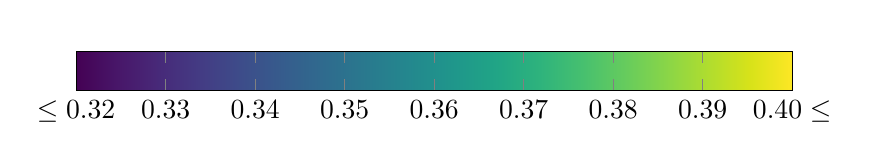
\begin{tikzpicture}
      \begin{axis}[
          hide axis,
          scale only axis,
          height=0pt,
          width=0pt,
          colormap/viridis,
          colorbar horizontal,
          point meta min=0.32,
          point meta max=0.40,
          colorbar style={
              width=0.75\textwidth,
              xtick={0.32, 0.33, 0.34, 0.35, 0.36, 0.37, 0.38, 0.39, 0.40},
              xticklabels={$\le 0.32$, $0.33$, $0.34$, $0.35$, $0.36$, $0.37$, $0.38$, $0.39$, $0.40 \le$}
          }]
          \addplot [draw=none] coordinates {(0,0)};
      \end{axis}
    \end{tikzpicture} 
    \begin{tikzpicture}[>=latex]
      \draw[thick, ->] (-6.5,0) -- (-6.5,-4.5) node[midway, above, rotate=90]{Time};
      \node (tube0) at (0,-0.0) {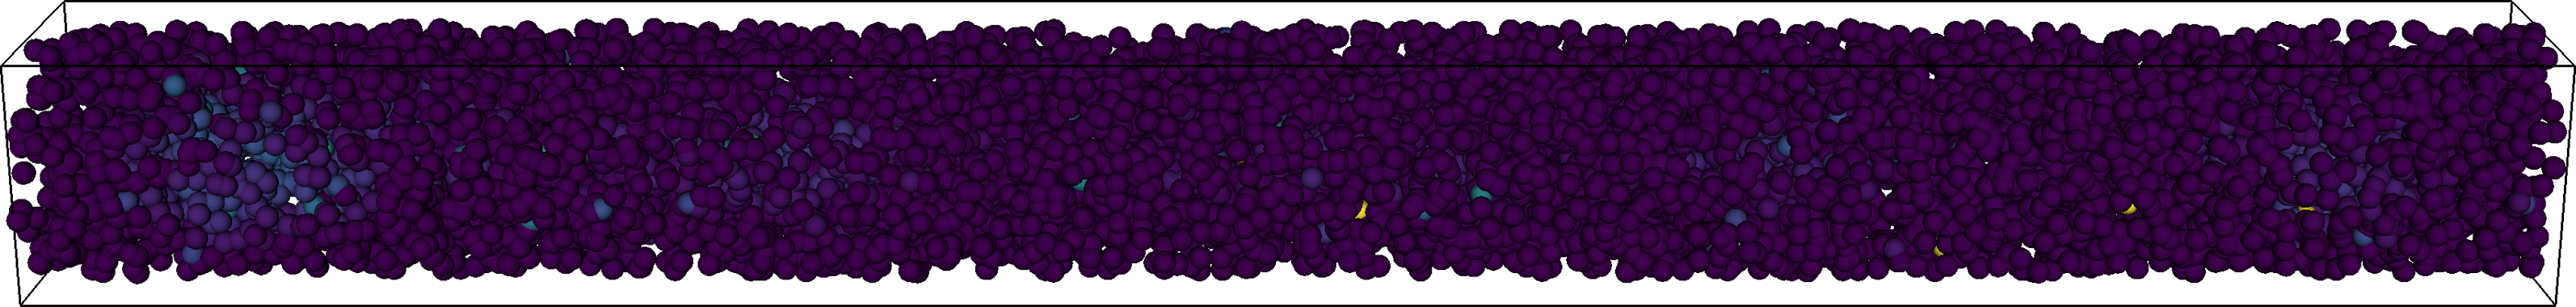
\includegraphics[width=0.9\textwidth]{figures/tube/tube_print_0}};
      \node (tube1) at (0,-1.5) {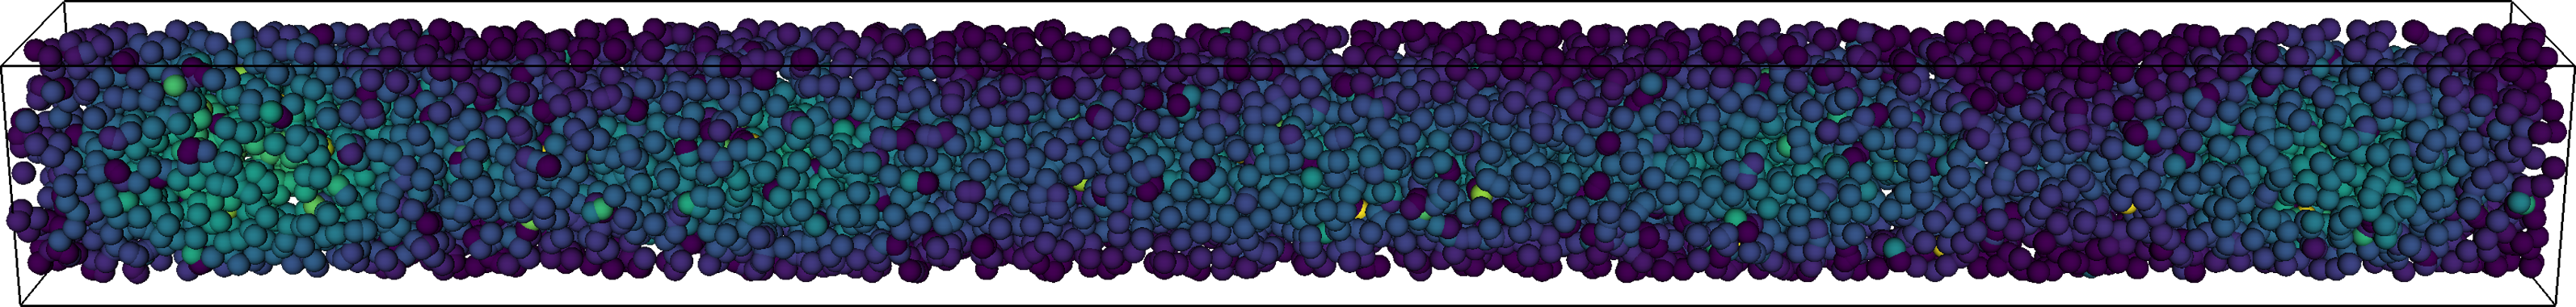
\includegraphics[width=0.9\textwidth]{figures/tube/tube_print_1}};
      \node (tube2) at (0,-3.0) {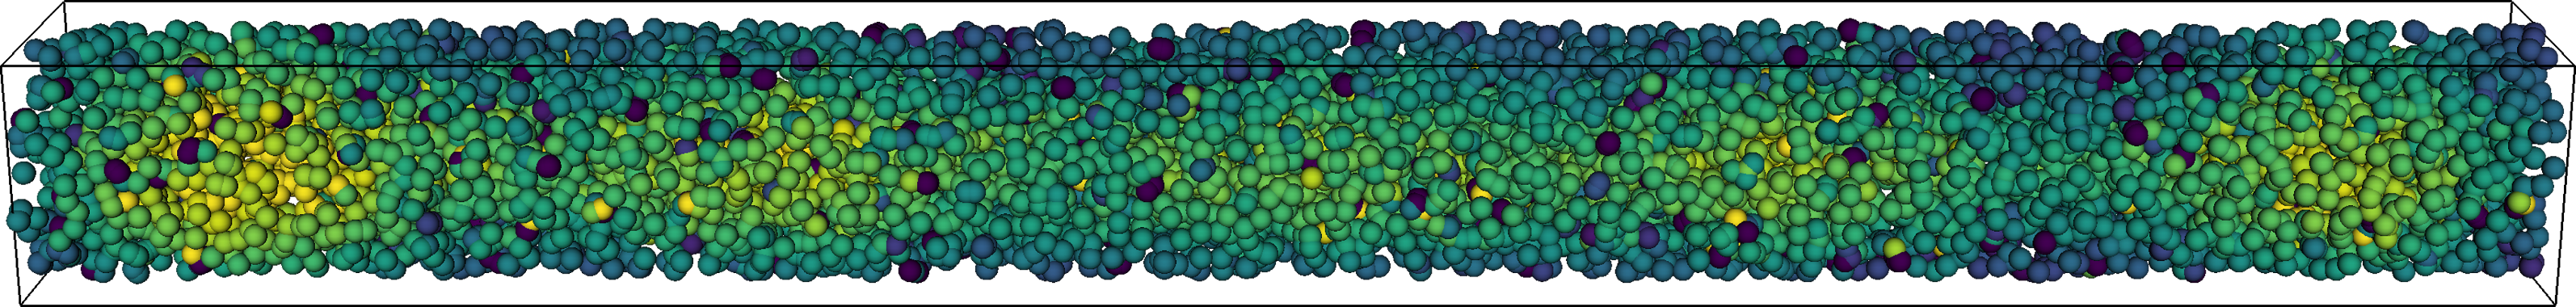
\includegraphics[width=0.9\textwidth]{figures/tube/tube_print_2}};
      \node (tube3) at (0,-4.5) {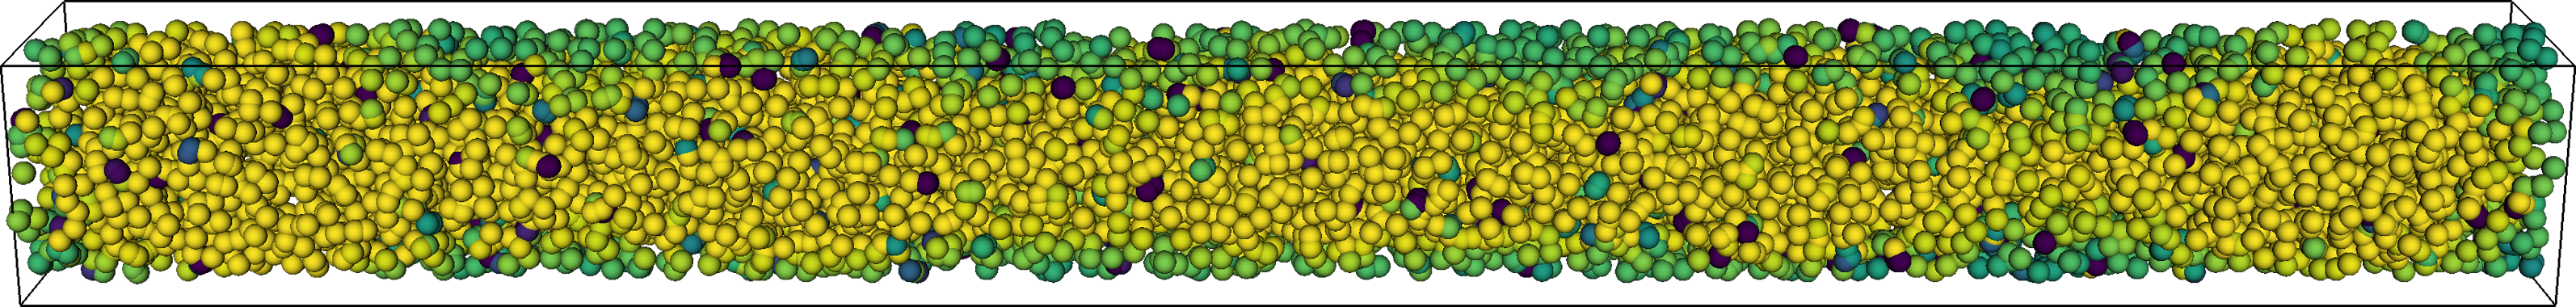
\includegraphics[width=0.9\textwidth]{figures/tube/tube_print_3}};
      %\draw[->] (6.5,0) -- (6.5,-4.5) node[midway, above, rotate=-90]{Time};
      \path[->] (7.5,0) -- (7.5,-4.5);
    \end{tikzpicture} 
  \end{center}
\end{frame}

\begin{frame}{Future work}
  \begin{itemize}
    \item Additional dynamical systems (nanomagnetics, biexcitons, degenerate states)
    \item Development of isotemporal model (same basis functions for integration, interpolation)
    \item Improved $\Lambda$ weighting ($\delta$-function representation in terms of Legendre polynomials?)
    \item Multi-level FFT-based propagation
    \item Extremely large systems (MPI and/or GPU)
  \end{itemize}
\end{frame}

\section{QuEST}

\begin{frame}{Software features}
  \begin{columns}
    \column{0.5\textwidth}
      \begin{itemize}
        \item Modern C++
        \item CMake
        \item Object-oriented
          \begin{itemize}
            \item Integrator, RHS function
            \item Interactions
            \item Assistance classes
          \end{itemize}
        \item Unit tests
        \item Additional tools
          \begin{itemize}
            \item Data manipulation
            \item Visualization
            \item Math
          \end{itemize}
        \item Clang-format
        \item Developed on git
      \end{itemize}

    \column{0.5\textwidth}
      \begin{center}
        \vspace{-0.5cm}
        \href{https://www.github.com/cglosser/quest}{
          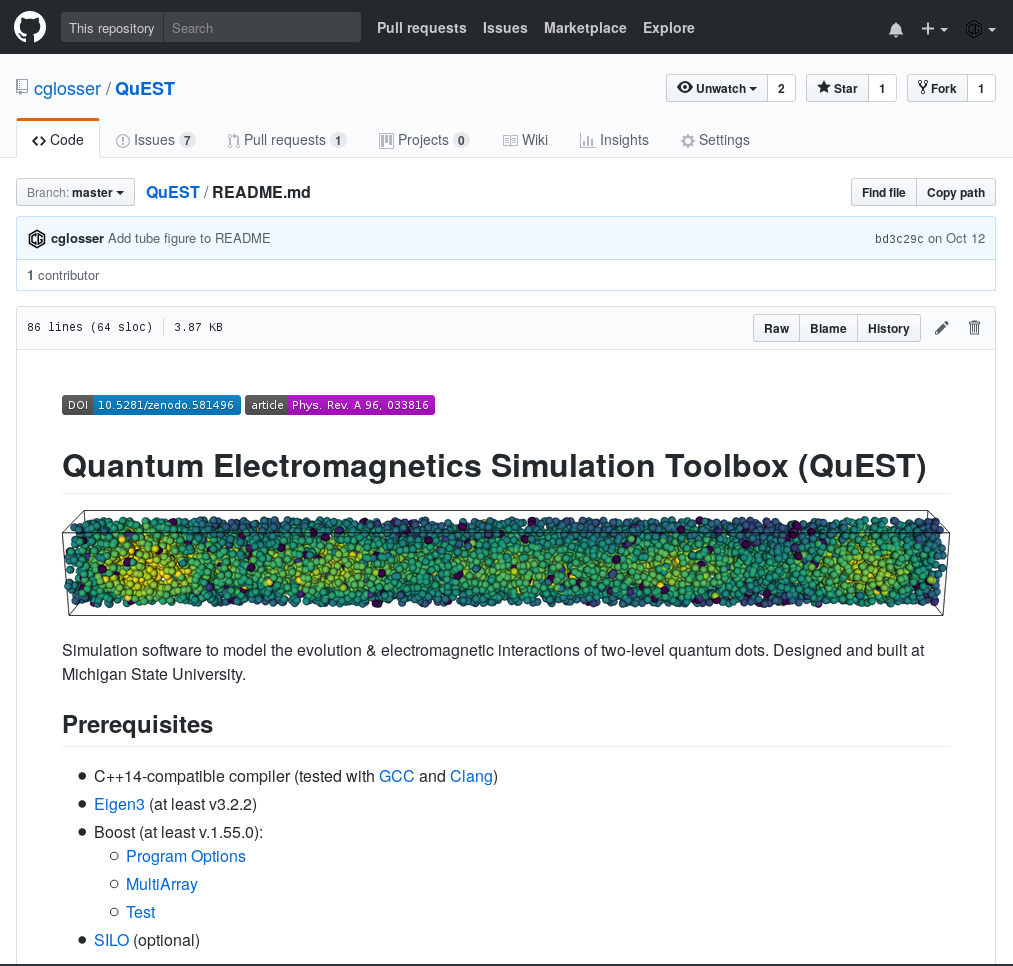
\includegraphics[width=\textwidth]{figures/github.png}
        }
        \url{https://github.com/cglosser/quest}
      \end{center}
  \end{columns}
\end{frame}

\begin{frame}{Hierarchy}
  \begin{center}
    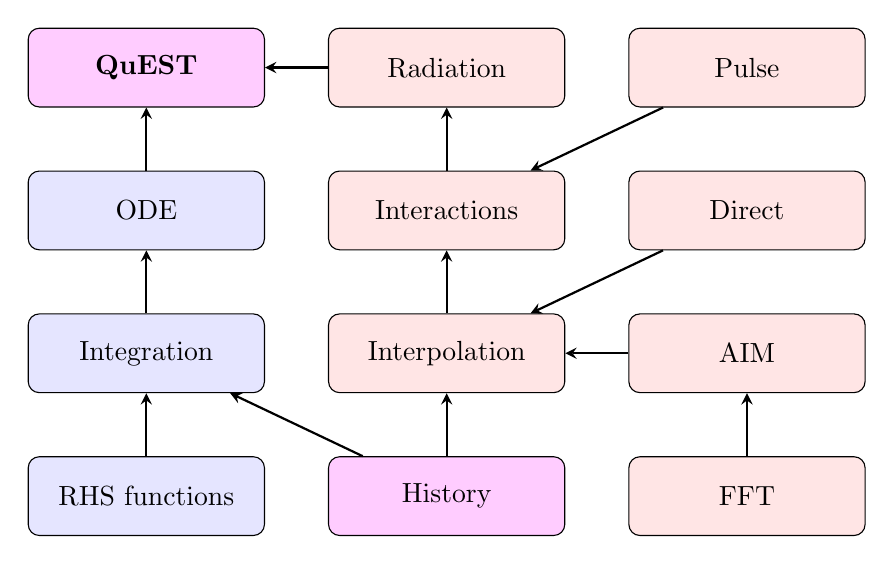
\begin{tikzpicture}[node distance=0.8cm, >=latex]
      \tikzstyle{physics} = [rectangle, rounded corners, minimum width=3cm, minimum height=1cm,text centered, draw=black, fill=blue!10]
      \tikzstyle{engineering} = [rectangle, rounded corners, minimum width=3cm, minimum height=1cm,text centered, draw=black, fill=red!10]
      \tikzstyle{both} = [rectangle, rounded corners, minimum width=3cm, minimum height=1cm,text centered, draw=black, fill=Fuchsia!20]
      \tikzstyle{arrow} = [thick,->,>=stealth]

      \node (quest) [both] {\textbf{QuEST}};
      \node (ode) [physics, below= of quest] {ODE};
      \node (radiation) [engineering, right= of quest] {Radiation};

      \draw [arrow] (ode) -- (quest);
      \draw [arrow] (radiation) -- (quest);

      \node (interactions) [engineering, below= of radiation] {Interactions};
      \node (integration) [physics, below= of ode] {Integration};
      \node (rhs) [physics, below= of integration] {RHS functions};
      \node (history) [both, right= of rhs] {History};

      \draw [arrow] (interactions) -- (radiation);
      \draw [arrow] (integration) -- (ode);
      \draw [arrow] (history) -- (integration);
      \draw [arrow] (rhs) -- (integration);

      \node (pulse) [engineering, right= of radiation] {Pulse};

      \draw [arrow](pulse) -- (interactions);

      \node (direct) [engineering, right= of interactions] {Direct};
      \node (interpolation) [engineering, below= of interactions] {Interpolation};
      \node (aim) [engineering, below= of direct] {AIM};

      \node (fft) [engineering, below= of aim] {FFT};

      \draw [arrow] (history) -- (interpolation);
      \draw [arrow] (interpolation) -- (interactions);
      \draw [arrow] (direct) -- (interpolation);
      \draw [arrow] (aim) -- (interpolation);
      \draw [arrow] (fft) -- (aim);

    \end{tikzpicture}
  \end{center}
\end{frame}

\begin{frame}{Things I've worked on}
  \begin{itemize}
    \item Radiation models (quantum optics: QuEST)
      \begin{itemize}
        \item Rank-deficient fast methods, performance optimization, tree codes, FFTs, GPUs
      \end{itemize}
    \item Molecular dynamics (hydrocarbon bonding, acoustic potentials)
    \item Nanostructure inverse problem/structure reconstruction (Tribond)
    \item Computational physics education
      \begin{itemize}
        \item \textbf{I}nternational \textbf{C}ourse in \textbf{C}omputational \textbf{P}hysics
        \item Course development, teaching assistantships
        \item Introductory workshops (highschool and college level)
      \end{itemize}
  \end{itemize}
\end{frame}
\appendix

\begin{frame}[standout]
  Questions?
\end{frame}

\begin{frame}{Units}
  \begin{table}
    \begin{tabular}{lll}
      Quantity                 & Symbol            & Value                        \\ \hline \hline
      Speed of light           & $c$               & \SI{300}{\micro\meter \per \pico\second} \\
      Transition frequency     & $\omega_0$        & $\SI{1500}{\milli\eV}/\hbar$ \\
      Transition dipole moment & $\vb{d}$          & \SI{10}{\elementarycharge\bohr} (uniform) \\
      Relaxation times         & $T_{1}, T_{2}$    & \SIlist{10;20}{\pico\second} \\
      Laser frequency          & $\omega_L$        & $\SI{1500}{\milli\eV}/\hbar$ \\
      Laser wavevector         & $\vb{k}_L$        & $\omega_L/c$ ($\vb{k}_L \cdot \vb{d} = 0$) \\
      Pulse width              & $\sigma/\omega_L$ & \SI{1}{\pico\second} \\ \hline
      Integrator window        & $W$               & 20 \\
      Corrector iterations     & N/A               & max 10 (usually 4-6) \\
      Timestep                 & $\Delta t$        & \SI{0.5e-2}{\pico\second}
    \end{tabular}
  \end{table}
\end{frame}

\begin{frame}{Lightning review of (linear) Green's functions}
  \only<1>{
    To solve the following differential equation for $a(x)$ \ldots
    \begin{equation*}
      \hat{\mathcal{L}}\qty[a(x)] = b(x)
    \end{equation*}
    \ldots it's far easier to \emph{first} find the Green's function,
    \begin{equation*}
      \hat{\mathcal{L}}\qty[g(x, x')] = \delta(x - x').
    \end{equation*}
    Then,
    \begin{align*}
      \hat{\mathcal{L}}\qty[a(x)] &= \int_{} \delta(x - x') b(x') \dd{x'} \\
                                  &= \int_{} \hat{\mathcal{L}}\qty[g(x, x')] b(x') \dd{x'} \\
                     \Aboxed{a(x) &= \int_{} g(x, x') b(x') \dd{x'}}
    \end{align*}
  }
  \only<2>{
    \begin{block}{Laplace equation}
      \begin{equation*}
        \laplacian g(\vb{r}, \vb{r}') = -4 \pi \delta(\vb{r} - \vb{r}') \implies g(\vb{r}, \vb{r}') = \frac{1}{\abs{\vb{r} - \vb{r}'}}
      \end{equation*}
    \end{block}

    \begin{block}{Wave equation}
      \begin{equation*}
        \qty(\laplacian - \frac{1}{c^2}\pdv[2]{t}) g^{(4)} = -4 \pi \delta^{(4)} \implies g(\vb{r}, t; \vb{r}', t') = \frac{1}{\abs{\vb{r} - \vb{r}'}} \delta\qty(t - t' - \frac{\abs{\vb{r} - \vb{r}'}}{c})
      \end{equation*}
    \end{block}
  }
\end{frame}

\begin{frame}{An electric-field wave equation}
  \vspace{0.7cm}
  \begin{columns}
    \column{0.6\textwidth}
        \begin{equation*}
          \laplacian{\pdv{\vb{E}}{t}} - \frac{1}{c^2} \pdv[3]{\vb{E}}{t} = 4 \pi k_2 \qty(\pdv[2]{\vb{J}}{t} - c^2 \grad \div \vb{J})
        \end{equation*}
        \begin{itemize}
          \item Incorporates short and long-range effects
          \item Automatic radiation boundary conditions
          \item Point-to-point communication; no numerical dispersion
          \item \alert{Four} derivatives, two spatial and two temporal
        \end{itemize}

    \column{0.4\textwidth}
      \centering
      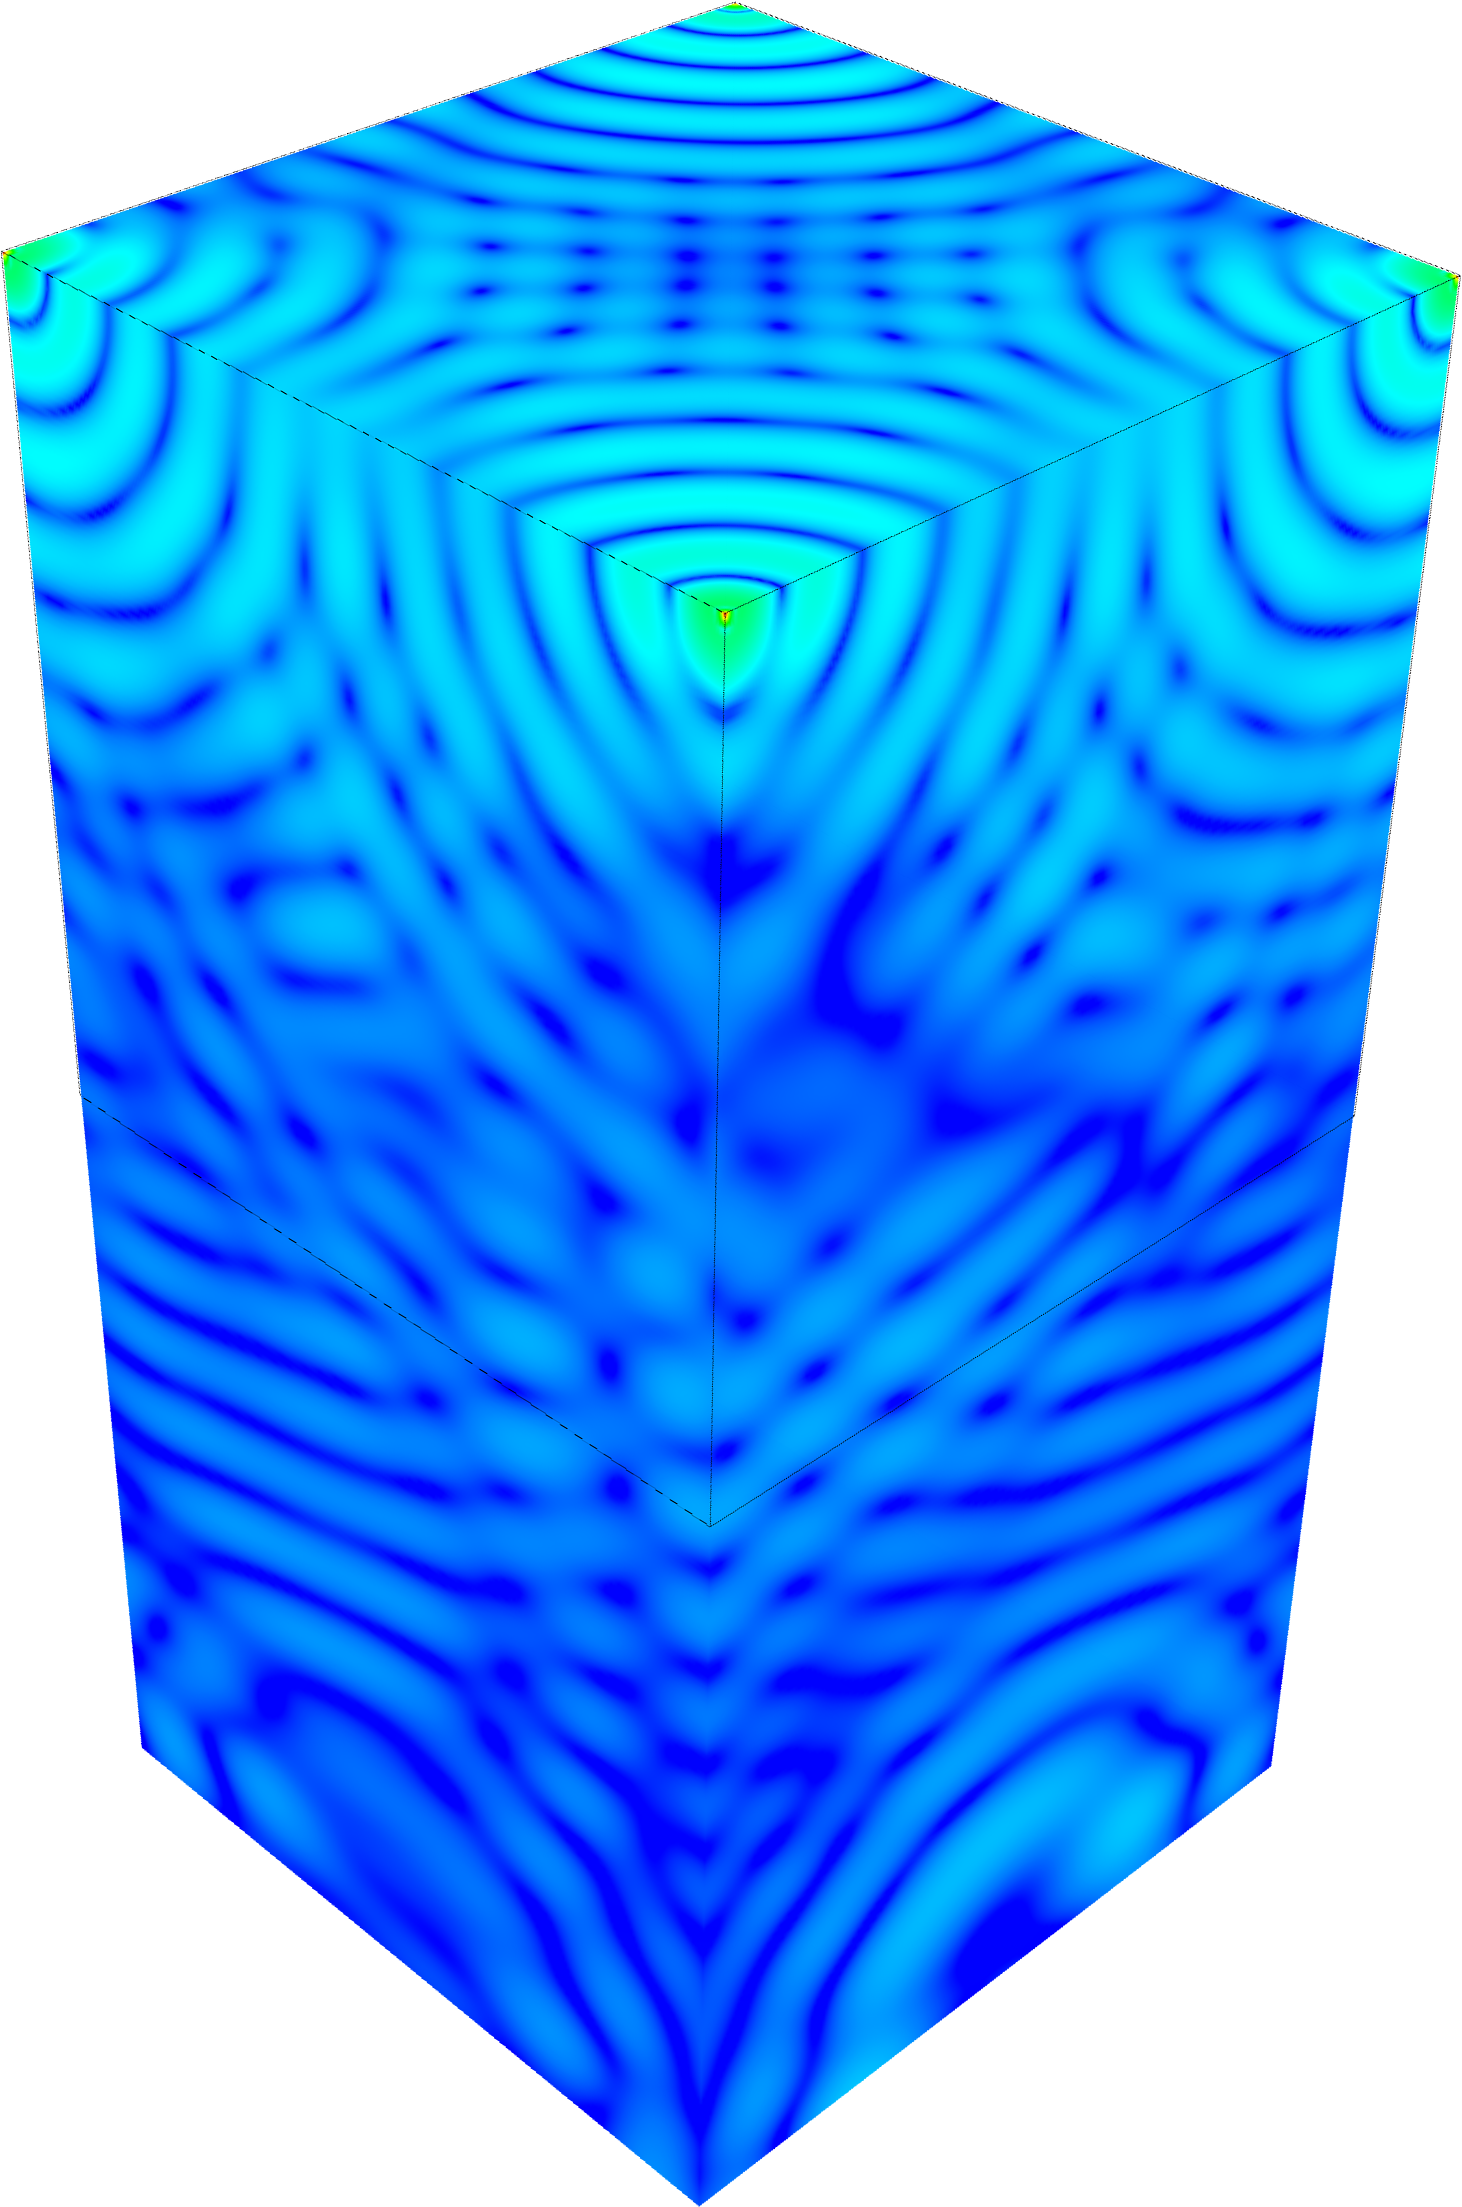
\includegraphics[width=0.5\textwidth]{figures/dipoles_2.png}
  \end{columns}

  \begin{equation*}
    \mathfrak{F}\qty{\vb{P}(\vb{r}, t)} = -k_2 \int_{}
        \left(\overline{\mathbf{I}} -  \hat{\mathbf{r}}\hat{\mathbf{r}}\right) \cdot \frac{\ddot{\mathbf{P}}(\vb{r}, t_R)}{\left|\mathbf{r}-\mathbf{r}'\right|} +
        \left(\overline{\mathbf{I}} - 3\hat{\mathbf{r}}\hat{\mathbf{r}}\right) \cdot \qty(
          \frac{c\dot{\mathbf{P}}(\vb{r}, t_R)}{\left|\mathbf{r}-\mathbf{r}'\right|^2} +
          \frac{c^2   \mathbf{P}(\vb{r}, t_R)}{\left|\mathbf{r}-\mathbf{r}'\right|^3}
        )
      \, \mathrm{d}^3 \mathbf{r'}
  \end{equation*}
\end{frame}

\begin{frame}{Classical electrodynamics: procedureally solving a matrix equation}
  \begin{block}{Marching-on-in-Time}
    \begin{equation*}
    \oper{L}^{(m)} + \sum_{k = 0}^m \oper{Z}^{(k)} \oper{A}^{(m-k)} = \oper{F}^{(m)}; \quad \oper{A}^{(m)}_n = \Trace\!\qty[\hat{\rho}_n(m \, \Delta t) \cdot \hat{\vb{d}}_n]
    \end{equation*}
  \end{block}

  \vspace{-0.5cm}
  \begin{equation*}
    \underbrace{\mqty(\oper{L}^{(0)} \\ \oper{L}^{(1)} \\ \oper{L}^{(2)} \\ \oper{L}^{(3)} \\ \oper{L}^{(4)})}_\text{Laser} +
    \underbrace{\mqty(
      \oper{Z}^{(0)} \\
      \oper{Z}^{(1)} & \oper{Z}^{(0)} \\
      \oper{Z}^{(2)} & \oper{Z}^{(1)} & \oper{Z}^{(0)} \\
      \oper{Z}^{(3)} & \oper{Z}^{(2)} & \oper{Z}^{(1)} & \oper{Z}^{(0)} \\
                                & \oper{Z}^{(3)} & \oper{Z}^{(2)} & \oper{Z}^{(1)} & \oper{Z}^{(0)} \\
      )}_\text{Interaction weights (precalculated)} \cdot
    \underbrace{\mqty(\oper{A}^{(0)} \\ \oper{A}^{(1)} \\ \oper{A}^{(2)} \\ \oper{A}^{(3)} \\ \oper{A}^{(4)})}_\text{Sources} =
    \underbrace{\mqty(\oper{F}^{(0)} \\ \oper{F}^{(1)} \\ \oper{F}^{(2)} \\ \oper{F}^{(3)} \\ \oper{F}^{(4)})}_\text{Total field}
  \end{equation*}

  \begin{equation*}
    \oper{L}^{(m)}_\ell = \langle\vb{S}_\ell(\vb{r}), \vb{E}_L (\vb{r}, m\, \Delta t)\rangle \quad
    \oper{Z}^{(k)}_{\ell\ell'} = \langle\vb{S}_\ell(\vb{r}), \mathfrak{F}\qty{\vb{S}_{\ell'}(\vb{r})T(k \, \Delta t)}\rangle \quad
    \oper{F}^{(m)}_\ell = \langle\vb{S}_\ell(\vb{r}), \vb{E} (\vb{r}, m\, \Delta t)\rangle
  \end{equation*}
\end{frame}

\begin{frame}{Interpolation influence}
  \begin{columns}
    \column{0.45\textwidth}
      \begin{center}
        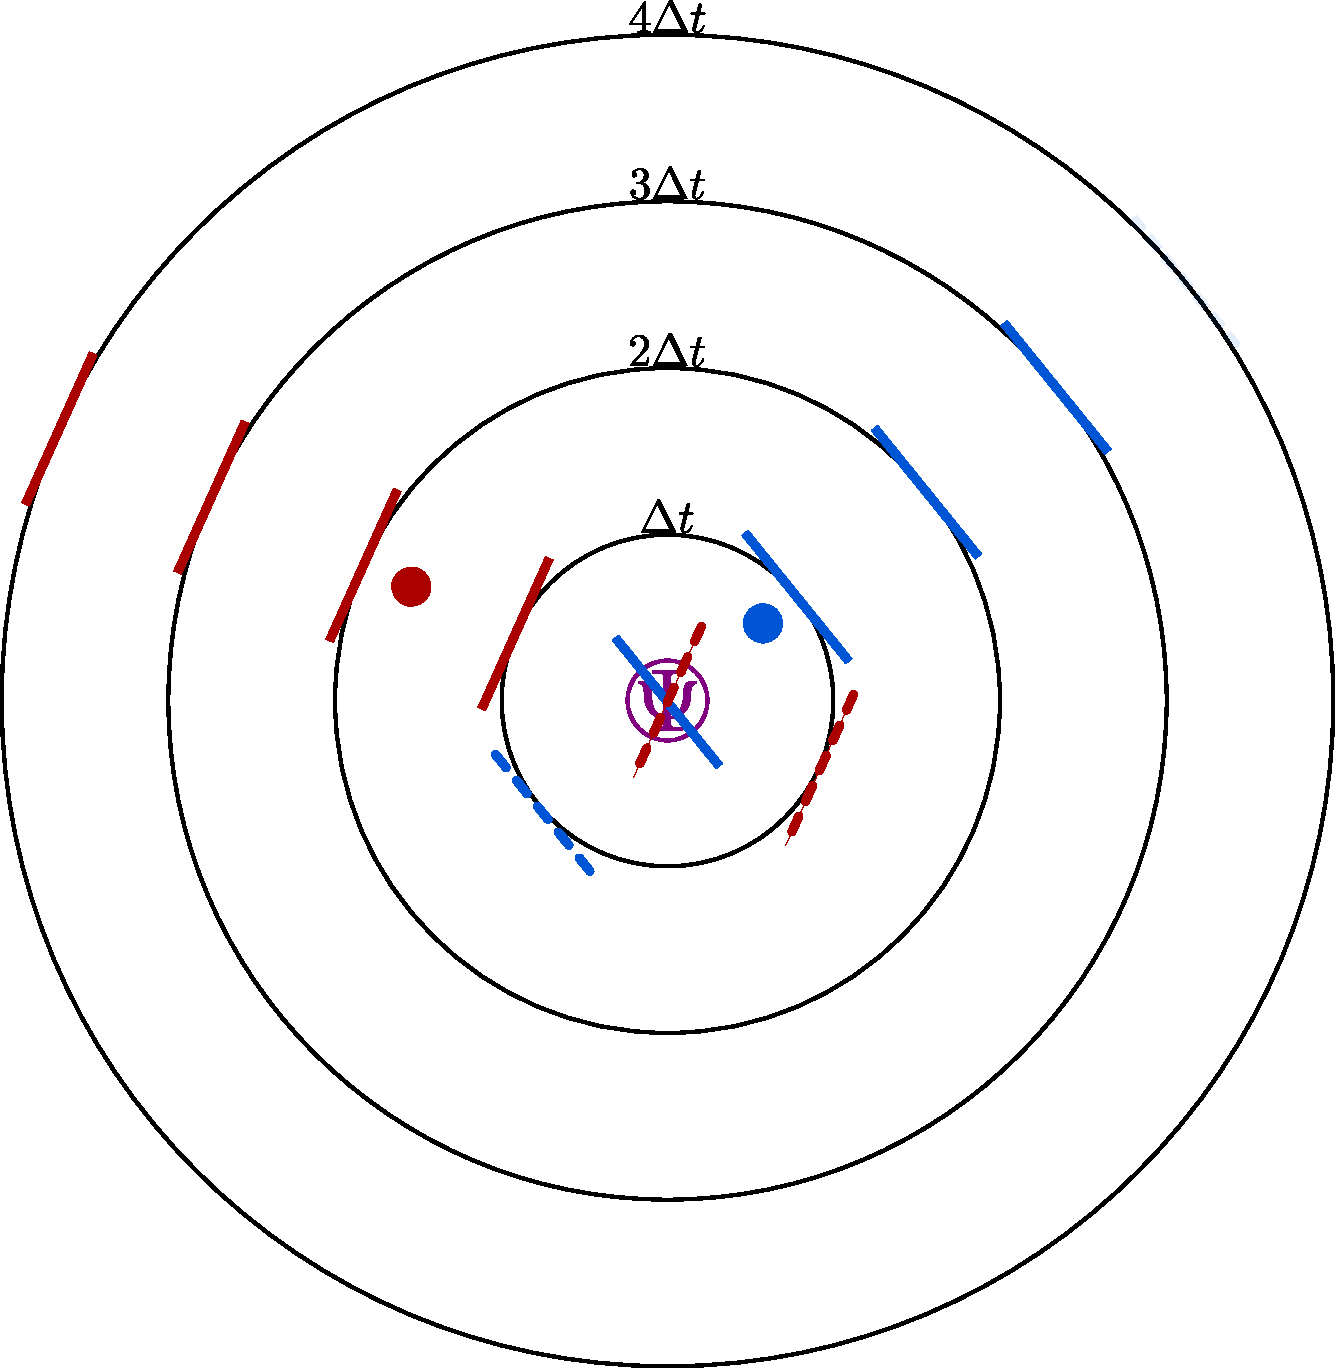
\includegraphics[height=0.85\textheight]{figures/spheres_of_influence}
      \end{center}

    \column{0.55\textwidth}
      \begin{itemize}
        \item Interpolate $\rho$, $\vb{P}$ due to $\abs{\vb{r} - \vb{r}'}/c \, \not \in \mathbb{N}$
        \item Sufficiently high order to recover $\partial_t^2 \vb{P}$, $\partial_t \vb{P}$, $\vb{P}$
        \item Time-domain solution imposes causality requirement: $T(t) = 0 \, \forall \, t < -1$
      \end{itemize}
  \end{columns}
\end{frame}

\begin{frame}{Simulated quantum dot = two-level quantum system}
  \begin{columns}
    \column{0.5\textwidth}
      \begin{block}{Liouville equation}
        \begin{equation*}
          \dv{\hat{\rho}}{t} = \frac{-i}{\hbar} \commutator{\hat{\mathcal{H}}(t)}{\hat{\rho}} - \hat{\mathcal{D}}\qty[\hat{\rho}]
        \end{equation*}
        \hfill {\tiny(mixed-state analogue of Schr\"odinger equation)}
      \end{block}

      \begin{itemize}
        \item Density matrix representation
        \item $\hat{\mathcal{D}}[\hat{\rho}]$ (phenomenologically) incorporates decay and decoherence
        \item Rabi oscillations
        \item One wavefunction/dot
          \begin{itemize}
            \item No universal wavefunction
            \item \emph{Classical} electromagnetic propagation
          \end{itemize}
      \end{itemize}

    \column{0.5\textwidth}
      \begin{center}
        \begin{filecontents}{example_bloch.dat}
0.                       0.                        0.                       -1.
0.004887585532746823   0.00009212990552802263    -0.000615646483982036    -0.9999998013063441
0.009775171065493646   0.0003676317912202054     -0.0012010282914746977   -0.9999992013693156
0.01466275659824047    0.00081913688170754       -0.0017152061870508778   -0.9999981788407986
0.019550342130987292   0.0014311451589153646     -0.0021188310912026655   -0.9999967116108025
0.024437927663734115   0.0021803630521431776     -0.002375645903243931    -0.9999947767125574
0.02932551319648094    0.0030362691713231678     -0.002453915675475679    -0.9999923503031307
0.03421309872922776    0.00396198361875489       -0.002327837131421285    -0.9999894076291549
0.039100684261974585   0.004915334014317273      -0.00197864418685883     -0.999985922995586
0.04398826979472141    0.005850155851215669      -0.0013956438469188233   -0.9999818697425832
0.04887585532746823    0.006717762136212471      -0.0005769432294939089   -0.9999772202077034
0.05376344086021505    0.007468556146095187      0.0004699136308808023    -0.9999719456867673
0.05865102639296188    0.008053743553067856      0.0017279121689583606    -0.9999660164265143
0.0635386119257087     0.008427070017187751      0.0031705511003610855    -0.9999594015750168
0.06842619745845552    0.008546547534876265      0.004762230519002424     -0.9999520691318996
0.07331378299120235    0.008376161917972373      0.006458938650232708     -0.9999439859262674
0.07820136852394917    0.007887447376718794      0.00820924886489589      -0.9999351175847436
0.08308895405669599    0.007060882235766189      0.009955621121639334     -0.9999254284848135
0.08797653958944282    0.005887044286284817      0.011635929386712191     -0.9999148817212796
0.09286412512218964    0.0043676602136004695     0.013185201723715945     -0.9999034390542588
0.09775171065493646    0.0025159519705781528     0.014537537172323619     -0.9998910608997763
0.10263929618768328    0.00035722952718118665    0.01562811301246128      -0.9998777062514802
0.1075268817204301     -0.0020711225003983372    0.01639539551064916      -0.9998633326412951
0.11241446725317693    -0.004720263085996062     0.016783230604284795     -0.9998478961058885
0.11730205278592375    -0.007530665424061154     0.016742829803075277     -0.9998313511498157
0.12218963831867058    -0.010433167805171891     0.016234720289108856     -0.9998136506959173
0.1270772238514174     -0.013350349256892281     0.015230758604422844     -0.9997947460021945
0.13196480938416422    -0.016198500118158647     0.01371555629924374      -0.999774586639562
0.13685239491691105    -0.018889714228689077     0.011687616528659558     -0.9997531204498735
0.14173998044965787    -0.02133410653054211      0.009160230014628349     -0.9997302934949316
0.1466275659824047     -0.02344231056476244      0.006162243088186926     -0.9997060499785847
0.15151515151515152    -0.025128191231926146     0.0027382105760085837    -0.9996803321857807
0.15640273704789834    -0.02631147110801985      -0.001052165619945122    -0.999653080453989
0.16129032258064516    -0.026920257247005357     -0.005134788300382488    -0.9996242331189525
0.16617790811339198    -0.02689358105365004      -0.009422252128168414    -0.9995937264460744
0.1710654936461388     -0.02618403642691218      -0.013815334063951275    -0.9995614945343392
0.17595307917888563    -0.024759737394905404     -0.018205286455350727    -0.9995274692852625
0.18084066471163245    -0.02260598147408562      -0.022476268809361592    -0.9994915803514248
0.18572825024437928    -0.019726641826210405     -0.026507978358138642    -0.9994537550713504
0.1906158357771261     -0.01614547083891873      -0.030178647578586657    -0.9994139183665787
0.19550342130987292    -0.011906594355624878     -0.033368375126711855    -0.9993719926726355
0.20039100684261972    -0.007074195652663397     -0.03596243503484473     -0.9993278979017498
0.20527859237536657    -0.0017319575826607778    -0.03785450005988514     -0.9992815513742617
0.2101661779081134     0.00401788428509731       -0.038949960827707845    -0.9992328677287885
0.2150537634408602     0.010056000162224075      -0.03916939085588829     -0.9991817588044863
0.219941348973607      0.01624850422028841       -0.03845128700964907     -0.9991281336060736
0.22482893450635386    0.022449657966167796      -0.03675451031082787     -0.9990718982376254
0.2297165200391007     0.02850487516417199       -0.034060437944687404    -0.9990129558201495
0.2346041055718475     0.03425419057375318       -0.03037509537976885     -0.9989512063585914
0.2394916911045943     0.03953627038834251       -0.025730254039708446    -0.9988865466649562
0.24437927663734115    0.04419250394582606       -0.02018363775419546     -0.9988188703097935
0.249266862170088      0.048071042392305266      -0.01381881631568288     -0.9987480675365302
0.2541544477028348     0.05103105474318558       -0.006744674504413299    -0.9986740251445752
0.2590420332355816     0.05294720370908772       0.000905779617170842     -0.9985966263478278
0.26392961876832845    0.05371343408035044       0.008978019013477612     -0.9985157507353782
0.2688172043010753     0.053246456200609575      0.01729880556179337      -0.9984312741872977
0.2737047898338221     0.051488952188961906      0.02567943208219103      -0.9983430687708815
0.2785923753665689     0.04841286451070309       0.033919528341989025     -0.9982510025714246
0.28347996089931574    0.04402142092948396       0.0418117384172769       -0.9981549396088745
0.2883675464320626     0.03835021839646214       0.04914661197462381      -0.9980547397749824
0.2932551319648094     0.03146790622453881       0.0557175084817501       -0.9979502587274729
0.2981427174975562     0.023476446195302696      0.061325878042417896     -0.9978413477390359
0.30303030303030303    0.01451051276455863       0.06578688565440435      -0.997727853531195
0.30791788856304987    0.004735120735712036      0.06893449356308576      -0.9976096182297095
0.31280547409579668    -0.00565700621048084      0.0706262360241722       -0.9974864792590507
0.31769305962854348    -0.016448656477663234     0.07074777600493765      -0.9973582692125007
0.32258064516129032    -0.027402013340341303     0.0692176808857138       -0.9972248156402872
0.32746823069403717    -0.03826388433099305      0.06599074649561221      -0.9970859409620931
0.33235581622678397    -0.048771291501069264     0.061060370817783045     -0.9969414623862336
0.33724340175953077    -0.058657189166912004     0.05446043292174599      -0.9967911917803743
0.3421309872922776     -0.06765674583792702      0.046266806557511114     -0.9966349354783022
0.34701857282502446    -0.07551417793378198      0.0365977631628225       -0.9964724940897086
0.35190615835777126    -0.08198931026369266      0.025612256441556895     -0.9963036624489755
0.35679374389051806    -0.08686383582940757      0.013507868425445695     -0.9961282294850158
0.3616813294232649     -0.08994748214739845      0.0005180043150411588    -0.9959459780595842
0.36656891495601175    -0.09108456656167696      -0.013091668330835839    -0.9957566847068327
0.37145650048875855    -0.09015901491525026      -0.027028755052795842    -0.9955601195448989
0.37634408602150535    -0.08709846125057595      -0.040980174810114706    -0.9953560461731711
0.3812316715542522     -0.08187777216608094      -0.05461850377543241     -0.9951442215161876
0.38611925708699904    -0.0745223358456391       -0.06760908197252467     -0.9949243955792761
0.39100684261974585    -0.06510995204784395      -0.07961800905130913     -0.9946963112368349
0.39589442815249265    -0.053770318988069096     -0.09032025566869621     -0.9944597041728732
0.40078201368523945    -0.04068407336129215      -0.09940750370916548     -0.9942143027231846
0.4056695992179863     -0.026080937345625485     -0.10659609601202845     -0.9939598276754029
0.4105571847507331     -0.010237015539230395     -0.11163557861628046     -0.9936959919555186
0.4154447702834799     0.006530643667473171      -0.11431579697822726     -0.993422500542589
0.4203323558162268     0.023870119586221945      -0.11447313548808861     -0.9931390503402665
0.4252199413489736     0.04140123688321975       -0.11199614338527633     -0.9928453299906427
0.4301075268817204     0.05872313260490603       -0.10683113691993865     -0.992541019569609
0.4349951124144672     0.07542322631733112       -0.09898611203983002     -0.9922257903589078
0.439882697947214      0.0910867919670439        -0.08853207574722        -0.9918993047766312
0.4447702834799609     0.10530632976856524       -0.0756037931840526      -0.9915612161894612
0.4496578690127077     0.11769133260945491       -0.06039955526387685     -0.9912111686673312
0.4545454545454545     0.12787888877295914       -0.04317998933162643     -0.9908487966153646
0.4594330400782014     0.13554317615135994       -0.024263295952927443    -0.9904737246963866
0.4643206256109482     0.14040420277592644       -0.004019755322283502    -0.9900855676696085
0.469208211143695      0.1422358992363621        0.017134664105759586     -0.9896839301585107
0.4740957966764418     0.14087482176003546       0.03874565669246184      -0.989268406233203
0.4789833822091886     0.13622553643907334       0.06033052372318295      -0.9888385794510826
0.4838709677419355     0.12826570912254479       0.08138824383314511      -0.9883940223971918
0.4887585532746823     0.11704946395567677       0.10141056818853961      -0.9879342966412755
0.4936461388074291     0.10270901961549943       0.11989370588978897      -0.9874589523382437
0.498533724340176      0.08545456843748747       0.1363503322307596       -0.9869675281046181
0.5034213098729228     0.06557215280710608       0.15032155132739386      -0.9864595507240682
0.5083088954056696     0.04342046012396805       0.16138921991663763      -0.9859345348271574
0.5131964809384164     0.01942410007829247       0.16918664357749458      -0.9853919827705052
0.5180840664711632     -0.00593330773487457      0.17340923633426988      -0.9848313843343081
0.5229716520039101     -0.03211821577870148      0.17382398271300223      -0.9842522165308367
0.5278592375366569     -0.058557671531926106     0.17027804994292237      -0.9836539431292136
0.5327468230694037     -0.08465155107052044      0.1627050811171482       -0.9830360145885919
0.5376344086021506     -0.10978567799390503      0.15112966220775076      -0.9823978677245019
0.5425219941348974     -0.13334554286601843      0.13567002145688092      -0.9817389254818647
0.5474095796676442     -0.15473051079941466      0.11653868662715838      -0.9810585966610896
0.552297165200391      -0.1733682651769742       0.09404102643920144      -0.9803562756156639
0.5571847507331378     -0.18872961226495155      0.06857208977951539      -0.979631341921149
0.5620723362658847     -0.20034242813862724      0.04061012097841496      -0.9788831600949792
0.5669599217986315     -0.2078043384781272       0.010707931548656003     -0.9781110794187756
0.5718475073313783     -0.21079433394642794      -0.020517147660509487    -0.9773144336578657
0.5767350928641252     -0.20908309109880557      -0.05239507417599767     -0.9764925407644511
0.581622678396872      -0.20254255032775104      -0.08421659461372542     -0.9756447024382157
0.5865102639296188     -0.19115222991411782      -0.11524882187748964     -0.9747702038946678
0.5913978494623656     -0.17500271597687767      -0.14475164392718276     -0.9738683136651572
0.5962854349951124     -0.15429733120671835      -0.17199437324939376     -0.9729382833144745
0.6011730205278593     -0.12935142629492266      -0.1962727542037305      -0.9719793471480126
0.6060606060606061     -0.10058977180959187      -0.21692664529564448     -0.9709907217824221
0.6109481915933529     -0.06854038324760531      -0.23335727974365345     -0.9699716058299505
0.61583577712609975    -0.033824831337575315     -0.24504283894645218     -0.9689211797419435
0.62072336265884655    0.002852904421073617      -0.2515528569770466      -0.9678386055237244
0.62561094819159335    0.040719679208437685      -0.2525610965866256      -0.9667230264411306
0.63049853372434015    0.07894841627925414       -0.24785731167145858     -0.9655735666207578
0.63538611925708696    0.11667563978447004       -0.23735677799774443     -0.9643893306534157
0.6402737047898338     0.15302084442873692       -0.22110531056900834     -0.9631694034712074
0.64516129032258064    0.18710607938962667       -0.19928226697885673     -0.9619128500763806
0.65004887585532745    0.21807597536378992       -0.17220084342429295     -0.9606187152519343
0.6549364613880743     0.24511831356161382       -0.14030581017995003     -0.959286023200492
0.6598240469208211     0.2674850877062561        -0.10416842483425345     -0.9579137770866304
0.6647116324535679     0.2845116134439786        -0.06447601880529398     -0.9565009589290007
0.6695992179863147     0.2956341859212385        -0.02201964874583531     -0.9550465293641516
0.6744868035190615     0.30040608111870426       0.02232055207248977      -0.9535494273683894
0.6793743890518084     0.2985118268650694        0.06759243683410861      -0.9520085699397963
0.6842619745845552     0.2897802209964501        0.11279133157232266      -0.9504228516162446
0.689149560117302      0.27419198732398536       0.156882355701724        -0.9487911443546027
0.6940371456500489     0.25188431595013555       0.19882340771337806      -0.9471122973549522
0.6989247311827957     0.22315258823101825       0.2375885648533345       -0.9453851368043078
0.7038123167155425     0.18844882467818325       0.2721919636054234       -0.9436084656043596
0.7086999022482893     0.14837752648522826       0.30171266412400605      -0.9417810629111013
0.7135874877810361     0.10368568699289363       0.3253181668559882       -0.9399016839749813
0.718475073313783      0.055249013171743126      0.3422858101406061       -0.93796906004954
0.7233626588465298     0.004055934395228222      0.3520224377313621       -0.9359818981721729
0.7282502443792766     -0.048811295384316236     0.3540818964639185       -0.9339388809431077
0.7331378299120235     -0.10219820398104422      0.34818123644565696      -0.9318386661302362
0.7380254154447703     -0.1549030791907436       0.3342125146317741       -0.9296798864604631
0.7429130009775171     -0.20570382446085064      0.3122491703009045       -0.927461149628184
0.7478005865102639     -0.2533850865316899       0.28254959151519793      -0.9251810381346511
0.7526881720430107     -0.2967659669855437       0.2455568299272872       -0.9228381091281879
0.7575757575757576     -0.3347286524288011       0.2018950744893733       -0.9204308941117566
0.7624633431085044     -0.3662470169952153       0.15236121512760822      -0.917957898698386
0.7673509286412512     -0.3904124253750524       0.09790979377630926      -0.9154176027236716
0.7722385141739981     -0.4064576059653264       0.03963564631160614      -0.9128084601725027
0.7771260997067449     -0.41377811545951554      -0.02124677132341753     -0.9101288990965216
0.7820136852394917     -0.41195170944490095      -0.08342728269403689     -0.907377321452723
0.7869012707722386     -0.40075513372157767      -0.1455273627320828      -0.9045521028633233
0.7917888563049853     -0.3801733164902316       -0.20613102912148148     -0.9016515928240594
0.7966764418377322     -0.3504050653819406       -0.2638161617722001      -0.8986741147546102
0.8015640273704789     -0.3118646002136097       -0.3171864781927488      -0.8956179660163577
0.8064516129032258     -0.265178794187745        -0.364904210219711       -0.8924814178996987
0.8113391984359727     -0.21118054712829154      -0.40572391681809206     -0.8892627154575009
0.8162267839687194     -0.15089358335564687      -0.43852362997517824     -0.8859600777907236
0.8211143695014663     -0.0855134743993869       -0.46233346119143454     -0.882571698265532
0.8260019550342132     -0.016385293312184412     -0.476361669286466       -0.8790957446606368
0.8308895405669599     0.055022589853874405      -0.48001783060887077     -0.8755303593187371
0.8357771260997068     0.12714837609890217       -0.47293429039231377     -0.8718736591332835
0.8406647116324537     0.19837134766531958       -0.4549800594131648      -0.8681237359037284
0.8455522971652004     0.2670479823794081        -0.4262687751516495      -0.8642786567592384
0.8504398826979473     0.3315485298224663        -0.38716255081081136     -0.8603364644715364
0.855327468230694      0.39029430697383133       -0.33827061642863165     -0.8562951777929674
0.8602150537634409     0.44179639037085866       -0.2804438867798376      -0.8521527916668982
0.8651026392961877     0.48469311814424054       -0.21476141874678825     -0.8479072776771827
0.8699902248289345     0.5177839879392081        -0.14250960535750903     -0.8435565847062481
0.8748778103616814     0.5400608909755992        -0.06515823474505546     -0.8390986394572902
0.879765395894428      0.5507359724879869        0.01566794096501116      -0.8345313470101751
0.884652981427175      0.5492671329024136        0.09822179784516592      -0.8298525913124681
0.8895405669599218     0.5353782679349801        0.18067138400854857      -0.8250602357832458
0.8944281524926686     0.5090700958176871        0.26114119994056934      -0.8201521242226456
0.8993157380254154     0.4706266779507811        0.33775376571622484      -0.8151260815937719
0.9042033235581623     0.4206161245860829        0.4086720370370077       -0.8099799148369932
0.909090909090909      0.3598859861222066        0.472142905740993        -0.8047114136845889
0.913978494623656      0.28955240281694083       0.5265413974510557       -0.799318351511205
0.9188660801564028     0.21097819454485728       0.5704107119374205       -0.7937984865079246
0.9237536656891495     0.12574714842080673       0.6024991051020727       -0.7881495627773608
0.9286412512218964     0.03563349791161527       0.6217931577304386       -0.782369311455685
0.9335288367546431     -0.05743350651103832      0.6275474173496829       -0.7764554518837722
0.93841642228739       -0.15140994445325595      0.6193111082911982       -0.7704056928157784
0.943304007820137      -0.2441833452799243       0.5969435340718066       -0.7642177338809069
0.9481915933528836     -0.333619816139814        0.560623317635937        -0.7578892670420677
0.9530791788856305     -0.4176118883056913       0.5108516896944335       -0.7514179780810151
0.9579667644183772     -0.4941271888806538       0.44844909581130654      -0.7448015481613286
0.9628543499511241     -0.5612588463002177       0.3745464401004714       -0.7380376554954479
0.967741935483871      -0.6172727486167098       0.29056419517485826      -0.7311239771555379
0.9726295210166177     -0.6606504527740666       0.19818440770722906      -0.7240581909311817
0.9775171065493646     -0.6901283280529125       0.09931823113825326      -0.7168379772370308
0.9824046920821115     -0.7047321643472086       -0.003932243403138467    -0.7094610211129742
0.9872922776148582     -0.7038090194588406       -0.10931737826427054     -0.7019250144192438
0.9921798631476051     -0.6870495887698327       -0.21449000286407668     -0.6942276581083843
0.997067448680352      -0.6545001440707241       -0.3170586360421731      -0.6863666645005086
1.0019550342130987     -0.6065687237240265       -0.4146409720272659      -0.6783397596727996
1.0068426197458456     -0.544023642757551        -0.5049182257593301      -0.6701446859510838
1.0117302052785923     -0.4679857010720205       -0.585691005861359       -0.661779204671278
1.0166177908113392     -0.37991028818161854      -0.6549344356248044      -0.6532410990616934
1.021505376344086      -0.28155717692818266      -0.7108475551653739      -0.6445281769507823
1.0263929618768328     -0.1749560329133832       -0.7518986084528917      -0.6356382736887496
1.0312805474095797     -0.06236566360186222      -0.776865304489405       -0.6265692551898123
1.0361681329423264     0.05377266289085307       -0.784870846719718       -0.6173190212742121
1.0410557184750733     0.17088834727674074       -0.775414134610545       -0.6078855093171938
1.0459433040078202     0.28634066719842843       -0.7483853883755767      -0.5982666974253136
1.0508308895405669     0.39747821509057957       -0.7040751301687486      -0.5884606079178294
1.0557184750733138     0.5016991339320238        -0.6431750443296504      -0.5784653109767196
1.0606060606060607     0.5965122160980925        -0.5667707463152383      -0.568278928577389
1.0654936461388074     0.6795993547741966        -0.47632693321422404     -0.5578996390161757
1.0703812316715543     0.748872167078484         -0.37365661359774305     -0.5473256806514216
1.0752688172043012     0.8025234343173727        -0.26088402131925337     -0.5365553559307918
1.0801564027370479     0.8390732284645704        -0.14040143103848693     -0.5255870356945413
1.0850439882697948     0.8574092106739146        -0.014819250300708223    -0.5144191637171364
1.0899315738025415     0.8568230508155836        0.113090242665973        -0.503050262125544
1.0948191593352884     0.8370320580456486        0.24045691063110963      -0.49147893589452163
1.0997067448680353     0.7981902852970821        0.36437860140112843      -0.4797038773507284
1.104594330400782      0.7408917987825346        0.48198716789607915      -0.46772387115601677
1.1094819159335289     0.6661644250551121        0.5905149868916795       -0.45553779948386114
1.1143695014662756     0.5754560277597417        0.6873631581505479       -0.4431446482535577
1.1192570869990225     0.47060589550614407       0.770166063962552        -0.43054351261658597
1.1241446725317693     0.35380436163490614       0.8368486841114041       -0.4177336018414191
1.129032258064516      0.2275471988045868        0.885678344542301        -0.4047142449659277
1.133919843597263      0.0945826595625761        0.915309674534202        -0.39148489662073316
1.1388074291300098     -0.042148172801913276     0.9248246885336022       -0.37804514393565425
1.1436950146627566     -0.1795788458483104       0.913762069999379        -0.36439471323673817
1.1485826001955034     -0.31458972631256343      0.8821301050362723       -0.35053347522909106
1.1534701857282503     -0.4440796158989243       0.8304118856661993       -0.3364614512451461
1.158357771260997      -0.5650376280267116       0.7595602271927715       -0.3221788196994207
1.163245356793744      -0.6746157620216117       0.6709834327167914       -0.30768592348290125
1.1681329423264906     -0.7702008003794132       0.5665198053588404       -0.2929832779852241
1.1730205278592375     -0.8494773651471044       0.4483946274161905       -0.2780715765603973
1.1779081133919844     -0.9104845539070991       0.3191716377450857       -0.2629516972056183
1.1827956989247311     -0.9516652631935487       0.18169718278317443      -0.2476247095825855
1.187683284457478      -0.9719083876539805       0.03903716096472613      -0.2320918827202516
1.1925708699902247     -0.9705843887787814       -0.10559322541679284     -0.2163546942543299
1.1974584555229716     -0.9475611618616359       -0.24890682081328253     -0.20041483629787663
1.2023460410557185     -0.9032098621100968       -0.3876215965597184      -0.18427422225899565
1.2072336265884652     -0.8384005656066738       -0.5185372867304616      -0.1679349942932263
1.2121212121212121     -0.7544870058679223       -0.6386115454239709      -0.15139953117169658
1.217008797653959      -0.6532833538550377       -0.7450380365085196      -0.13467045915406956
1.2218963831867057     -0.5370162486923872       -0.8353110947571394      -0.11775065541263845
1.2267839687194526     -0.408278781432947        -0.9072899881192337      -0.10064325805528032
1.2316715542521995     -0.26996964886263763      -0.9592519356845135      -0.08335167392644272
1.2365591397849462     -0.1252256793489543       -0.9899361887331289      -0.0658795851397664
1.2414467253176931     0.0226521730790204        -0.9985769870681276      -0.04823095834534067
1.2463343108504398     0.1702774243746248        -0.9849246163874782      -0.03041005188666283
1.2512218963831867     0.3142593062620826        -0.949253914733529       -0.012421423452248516
1.2561094819159336     0.45128481033165857       -0.892360196335544       0.0057300613751940545
1.2609970674486803     0.5781982104717458        -0.8155403448957375      0.02403922321816454
1.2658846529814272     0.6920798813742757        -0.720566466927973       0.04250055849383231
1.2707722385141739     0.7903166124999856        -0.6096411760661162      0.06110823402624433
1.2756598240469208     0.8706661894410618        -0.4853458567346046      0.07985607915212235
1.2805474095796677     0.9313127155612149        -0.3505783635211526      0.09873757822605676
1.2854349951124144     0.9709114999753292        -0.20848257443894752     0.11774586372031165
1.2903225806451613     0.9886222969383736        -0.06237153909193963     0.1368737090318195
1.2952101661779082     0.9841298362100541        0.08435383860662185      0.1561135220144082
1.3000977517106549     0.9576520553215303        0.22828862489787696      0.17545733780524198
1.3049853372434018     0.9099332442450607        0.36610796667470674      0.19489681305706075
1.3098729227761487     0.8422250696788126        0.4946491827863021       0.21442321989239252
1.3147605083088954     0.7562543279673125        0.6109898707655823       0.23402743976857365
1.3196480938416423     0.6541785799600263        0.7125199373028156       0.2536999584526354
1.324535679374389      0.5385307691507266        0.7970056397273313       0.27343086055522414
1.3294232649071359     0.4121542271405713        0.8626439460722151       0.2932098250731819
1.3343108504398828     0.2781298536144256        0.9081063459071792       0.3130261203726054
1.3391984359726295     0.13969664174196278       0.9325674980822738       0.33286860219957887
1.3440860215053764     0.00016969970737015783    0.9357258114984431       0.35272570800815795
1.348973607038123      -0.1371451335996876       0.9178066015409245       0.3725854546113553
1.35386119257087       -0.26903545013034635      0.8795520418257854       0.3924354363036011
1.3587487781036169     -0.3924635979393679       0.8221978919935782       0.4122628227166519
1.3636363636363636     -0.5046430961548866       0.7474373802509464       0.43205435772078793
1.3685239491691105     -0.6031080723217233       0.6573731716554457       0.45179635874603263
1.3734115347018573     -0.6857738791628526       0.5544587372985986       0.4714747166940057
1.378299120234604      -0.7509874132846539       0.441430753362239        0.4910748965511646
1.383186705767351      -0.7975669336794623       0.321234056296157        0.5105819375975906
1.3880742913000978     -0.8248234531932694       0.1969406395955629       0.5299804588187594
1.3929618768328446     -0.8325754706504774       0.07166765118989266      0.5492546591045488
1.3978494623655914     -0.8211459185608886       -0.05150657671318253     0.5683883222820004
1.4027370478983382     -0.7913461435711777       -0.16962445964281042     0.5873648211073047
1.407624633431085      -0.7444464644196381       -0.279927047162489       0.6061671236903501
1.412512218963832      -0.6821342073770491       -0.3799256793562998      0.6247777994684318
1.4173998044965786     -0.6064605274323389       -0.46746541440181205     0.6431790273310971
1.4222873900293255     -0.51977791679166         -0.5407795326762689      0.6613526029484524
1.4271749755620722     -0.4246676798215273       -0.5985271293345203      0.6792799521351508
1.4320625610948191     -0.3238662629333537       -0.6398285785613488      0.6969421366788875
1.436950146627566      -0.2201830103981117       -0.6642779543035461      0.7143198689527189
1.4418377321603127     -0.11641939895516559      -0.6719440925150455      0.7313935254418724
1.4467253176930596     -0.015289071344878613     -0.6633600046789888      0.7481431603642262
1.4516129032258065     0.08065920599304398       -0.6394977089312411      0.7645485205356042
1.4565004887585532     0.16911318405422981       -0.6017301598837724      0.780589062558556
1.4613880742913001     0.24805814269213666       -0.5517794048307088      0.7962439721929202
1.466275659824047      0.31583157685277957       -0.4916591832044114      0.8114921824357709
1.4711632453567937     0.37116471061099193       -0.42360662020653206     0.8263123947425234
1.4760508308895406     0.4132118122547257        -0.35000856055964574     0.84068310133564
1.4809384164222873     0.44156608546585563       -0.27332419184208523     0.8545826087502341
1.4858260019550342     0.4562616938500795        -0.19600636152550016     0.8679890629994542
1.4907135874877811     0.45776231095022574       -0.12042379994662841     0.8808804759177316
1.4956011730205278     0.44693424716122526       -0.04878794124489245     0.893234753508929
1.5004887585532747     0.4250103866629635        0.016915797413680073     0.905029725204747
1.5053763440860214     0.3935401880681814        0.07498802618594148      0.9162431746649189
1.5102639296187683     0.3543304047554445        0.1240655998129596       0.9268528727396712
1.5151515151515152     0.3093778242374194        0.16315975009089295      0.9368366111886537
1.5200391006842619     0.26079664138355074       0.19168171599667225      0.9461722383027389
1.5249266862170088     0.21074262921786008       0.20945442448874177      0.9548376957098863
1.5298142717497557     0.16133606792490843       0.21671224101420777      0.9628110575319253
1.5347018572825024     0.11458663894569032       0.21408330746126528      0.970070569611994
1.5395894428152493     0.07232242853381597       0.20256099782353262      0.9765946915842209
1.5444770283479962     0.03612555702218909       0.18346188748813289      0.9823621395929449
1.5493646138807429     0.0072765720473435686     0.15837271509600484      0.9873519308905865
1.5542521994134898     -0.013290466422927897     0.12908794162318568      0.9915434294540052
1.5591397849462365     -0.02502064217340768      0.09753996942441032      0.9949163933678793
1.5640273704789834     -0.027757387341870627     0.06572436097422765      0.9974510231190765
1.5689149560117303     -0.021747492175478222     0.0356225786945585       0.9991280115654955
1.573802541544477      -0.007631632468274189     0.009124882278216173     0.9999285947871045
1.5786901270772237     0.01357938285905474       -0.012043958125841135    0.9998346043701002
1.5835777126099706     0.04054196497889989       -0.02639353580824558     0.9988285205926848
1.5884652981427175     0.07162954870738304       -0.032728821657067406    0.996893526771528
1.5933528836754644     0.10499326311347458       -0.030201104864356315    0.9940135644672676
1.5982404692082113     0.13863149350700338       -0.018346956780575796    0.9901733896001896
1.6031280547409578     0.17046603036935667       0.0028863061715654423    0.9853586293064429
1.6080156402737047     0.19842224082181112       0.033129748800119645     0.9795558394682281
1.6129032258064516     0.22051052185864298       0.07159714063883406      0.9727525628025221
1.6177908113391985     0.23490620576955698       0.11710457631903043      0.9649373873855019
1.6226783968719453     0.24002509396792765       0.16810497137506034      0.9561000055047799
1.6275659824046922     0.23459189580498618       0.22273649629403625      0.9462312726925929
1.6324535679374388     0.21769904347866625       0.2788835177104798       0.9353232668184204
1.6373411534701857     0.1888536374429148        0.33424816127735546      0.9233693470825812
1.6422287390029325     0.14801064151566204       0.38643021137211736      0.9103642127693233
1.6471163245356794     0.09559088224810018       0.43301273340569013      0.8963039615919981
1.6520039100684263     0.03248289999729345       0.4716505572524146       0.8811861474691611
1.656891495601173      -0.039971766012548954     0.5001586054954166       0.8650098375544036
1.6617790811339198     -0.12000971670307696      0.5165969947144567       0.8477756683414563
1.6666666666666666     -0.20549254827475386      0.5193498860173777       0.8294859006564139
1.6715542521994135     -0.2939681621660429       0.5071952128513147       0.8101444733438937
1.6764418377321604     -0.38274474691857824      0.47936266693053403      0.789757055447572
1.6813294232649073     -0.46897517751683904      0.4355776703620676       0.7683310966794458
1.686217008797654      -0.5497491734640436       0.37608949396124836      0.7458758759673993
1.6911045943304007     -0.6221902349642762       0.3016821853789531       0.7224025478649462
1.6959921798631476     -0.6835541498246598       0.21366753037681252      0.6979241866031907
1.7008797653958945     -0.7313257418508099       0.11385986845010782      0.6724558275603796
1.7057673509286414     -0.763310520977807        0.004533200390333094     0.6460145059214606
1.710654936461388      -0.7777179988991271       -0.11163836041439999     0.6186192922967537
1.715542521994135      -0.7732336504042175       -0.23165515021782535     0.590291325066832
1.7204301075268817     -0.7490768249928901       -0.3522793411039105      0.5610538392189515
1.7253176930596286     -0.7050423367473898       -0.47013247845524486     0.5309321914395789
1.7302052785923755     -0.641523970448194        -0.5818000957075404      0.49995388122741286
1.735092864125122      -0.5595187227803774       -0.6839400283807286      0.4681485677920195
1.739980449657869      -0.46061123065619064      -0.7733908552048776      0.4355480825047008
1.7448680351906158     -0.34693850341050464      -0.8472768188385462      0.4021864366707679
1.7497556207233627     -0.22113574958544543      -0.9031056272954857      0.36809982439563804
1.7546432062561096     -0.08626474907004718      -0.9388557106417653      0.33332662032165183
1.759530791788856      0.054273155668378134      -0.9530498023657047      0.2979073720177862
1.764418377321603      0.1968368120161459        -0.9448121233118376      0.26188478681092836
1.76930596285435       0.33765463281736424       -0.9139069563239576      0.22530371285484657
1.7741935483870968     0.47294009012002364       -0.8607569960560203      0.18821111424158005
1.7790811339198437     0.5990095515863676        -0.7864405217210757      0.15065603996973442
1.7839687194525906     0.7123985394468771        -0.6926671490310642      0.11268958659511084
1.788856304985337      0.8099724805775589        -0.5817326473494557      0.07436485440113495
1.793743890518084      0.8890281413246698        -0.4564540339896652      0.03573689693980552
1.798631476050831      0.9473822003413687        -0.32008685410334076     -0.003137336191495232
1.8035190615835778     0.9834438003934722        -0.17622719667123773     -0.042199063456477906
1.8084066471163247     0.9962684246158297        -0.028701561100214785    -0.08138774247177327
1.8132942326490712     0.9855910484588991        0.11855184651642892      -0.12064114816818386
1.818181818181818      0.9518372060335107        0.2616064615623558       -0.15989545808601047
1.823069403714565      0.8961113559066922        0.3966712128590905       -0.1990853448486427
1.827956989247312      0.82016262564075          0.520210583263086        -0.2381440759600866
1.8328445747800588     0.7263291828913171        0.6290568947805709       -0.2770036205347762
1.8377321603128056     0.6174628613942563        0.7205112920592456       -0.31559476275607024
1.8426197458455522     0.4968356351274686        0.792428609156554        -0.3538472238104074
1.847507331378299      0.3680322257130024        0.8432841257032876       -0.3916897904610198
1.852394916911046      0.23483199894603707       0.8722195313696013       -0.4290504497596208
1.857282502443793      0.1010841443263043        0.8790663738578437       -0.4658565310577609
1.8621700879765397     -0.02941950679491142      0.8643459089594417       -0.502034854792537
1.8670576735092863     -0.15307001151511312      0.8292461408181097       -0.5375118870462284
1.871945259042033      -0.2665600194455981       0.775574396157021        -0.5722139013954918
1.87683284457478       -0.3669920893877826       0.7056896369444401       -0.6060671463701425
1.881720430107527      -0.4519723924781247       0.6224151712561632       -0.6389980182867993
1.886608015640274      -0.5196863375430485       0.5289353104930019       -0.6709332403081818
1.8914956011730204     -0.5689534983515631       0.42867965059748514      -0.7018000455962944
1.8963831867057673     -0.5992603688286459       0.325198871729341        -0.7315263669971046
1.901270772238514      -0.610766416492704        0.2220370997284011       -0.7600410259905099
1.906158357771261      -0.6042899955865884       0.12260474085532204      -0.7872739328177066
1.911045943304008      -0.5812673174268198       0.030056674317565257     -0.8131562840361285
1.9159335288367545     -0.5436909991861913       -0.05282099966212332     -0.8376207708823857
1.9208211143695014     -0.49402422856021333      -0.12370613327949531     -0.8606017738647562
1.9257086999022482     -0.43510297820092353      -0.1808224196898113      -0.8820355759512021
1.930596285434995      -0.3700218779753126       -0.22300102786007614     -0.9018605788062752
1.935483870967742      -0.3020095609207284       -0.24971250674163353     -0.9200174955077881
1.940371456500489      -0.23430171062189076      -0.2610812014389107      -0.9364495682436751
1.9452590420332354     -0.17001289151817625      -0.25787153458293727     -0.9511027741721542
1.9501466275659823     -0.11201343397301788      -0.24145020555103383     -0.9639260320163417
1.9550342130987292     -0.06281560023483007      -0.21372528814109898     -0.9748714079817523
1.959921798631476      -0.02447363425530836      -0.17706366395351253     -0.9838943184757354
1.964809384164223      0.0014976617477610102     -0.13419015456665767     -0.9909537258943049
1.9696969696969695     0.014183388827826576      -0.08807273716030052     -0.9960123320991964
1.9745845552297164     0.013305451787192115      -0.04179782499297051     -0.9990367667141112
1.9794721407624633     -0.0007657155381278541    0.0015596494000755488    -0.9999977696102679
1.9843597262952102     -0.027025245273572234     0.03906635063720612      -0.9988703666711848
1.989247311827957      -0.0638733891263513       0.06805580869537872      -0.9956340382042971
1.994134897360704      -0.10917901893585462      0.08624423835732617      -0.9902728819016988
1.9990224828934505     -0.1603656997822577       0.09183185479295408      -0.9827757638504715
2.0039100684261974     -0.21451655591942484      0.08358507262269144      -0.97313645695368
2.0087976539589443     -0.2684936179822391       0.06089692836182247      -0.9613537710850732
2.0136852394916912     -0.31906743236769747      0.023822964956892234     -0.9474316719116599
2.018572825024438      -0.3630519648037748       -0.026909114326965626    -0.9313793875281422
2.0234604105571846     -0.3974395612649359       -0.08991670418404286     -0.9132115021712673
2.0283479960899315     -0.4195306849836805       -0.16320607079356997     -0.8929480366428246
2.0332355816226784     -0.42705365247133725      -0.2442410939856889      -0.870614517804552
2.0381231671554253     -0.4182688229978225       -0.33003558108872655     -0.8462420280217178
2.043010752688172      -0.3920527184850553       -0.41726490715138        -0.8198672376644293
2.0478983382209187     -0.3479591824425792       -0.5023926778429452      -0.7915324239213304
2.0527859237536656     -0.28625469328705383      -0.5818079065823012      -0.7612854729379703
2.0576735092864125     -0.2079260943510115       -0.651967470358592       -0.7291798647410448
2.0625610948191594     -0.11466006354514961      -0.7095383357333067      -0.6952746405042733
2.0674486803519063     -0.008794809638609666     -0.7515340263723399      -0.6596343523335616
2.0723362658846528     0.10675440540625897       -0.7754403477266314      -0.6223289977082217
2.0772238514173997     0.2285944246358049        -0.7793243295435649      -0.5834339289557827
2.0821114369501466     0.35297330210495037       -0.7619220004959341      -0.5430297443537583
2.0869990224828935     0.4759150111815242        -0.7227018422525271      -0.5012021621938693
2.0918866080156404     0.5933649285906134        -0.6619009598137748      -0.4580418757522126
2.0967741935483872     0.7013405723487321        -0.5805322115836473      -0.41364438914771046
2.1016617790811338     0.796081801006712         -0.48036165858262425     -0.36810983415433135
2.1065493646138807     0.874194703711278         -0.36385695598034923     -0.32154276879632265
2.1114369501466276     0.9327839560476732        -0.23410832387961544     -0.2740519589209207
2.1163245356793745     0.9695671801148427        -0.09472378603214104     -0.2257501359134524
2.1212121212121213     0.982967075929458         0.050296133132415016     -0.1767537381957915
2.126099706744868      0.9721779053057699        0.19669983371843944      -0.12718263631275917
2.1309872922776148     0.9372033431511634        0.3401370354388065       -0.07715984100697065
2.1358748778103617     0.878863955797108         0.4763163389914876       -0.0268111949017593
2.1407624633431085     0.7987737397286044        0.6011618905777667       0.023734951507410486
2.1456500488758554     0.699286528395672         0.7109631684627914       0.07434807831630771
2.1505376344086023     0.5834139033810405        0.802512407524096        0.1248958489663276
2.155425219941349      0.45471665636798697       0.8732229173435061       0.17524447843107727
2.1603128054740958     0.317175342466589         0.9212242065583152       0.22525911182660294
2.1652003910068426     0.1750444624028096        0.9454302780660098       0.27480421369941027
2.1700879765395895     0.03269574255860979       0.9455781581765541       0.3237439671521415
2.1749755620723364     -0.10554342279759621      0.9222349915120344       0.3719426815812484
2.179863147605083      -0.23555006775428328      0.8767732669133841       0.4192652077397222
2.18475073313783       -0.3535579725754623       0.8113150357936793       0.46557735850017645
2.1896383186705767     -0.4562980887015169       0.728648162191282        0.5107463404764075
2.1945259042033236     -0.541114819444638        0.6321125891936545       0.554641174416584
2.1994134897360705     -0.6060618680182451       0.5254699869250231       0.5971331280537389
2.204301075268817      -0.6499725115040533       0.4127556355747525       0.6380961578744098
2.209188660801564      -0.6724901518490699       0.29811828988802974      0.6774073178627168
2.214076246334311      -0.6740765498838808       0.18565814846569798      0.7149472007179085
2.2189638318670577     -0.6559828520264837       0.07926545333113214      0.7506003598121814
2.2238514173998046     -0.6201880991659072       -0.017530752299641846    0.7842557169539836
2.228739002932551      -0.5693104860227131       -0.10169892862995505     0.8158069694127867
2.233626588465298      -0.506492988159865        -0.17082082955612338     0.8451529862194573
2.238514173998045      -0.43526819835532643      -0.22318220529658844     0.872198193667136
2.2434017595307918     -0.35940754313401096      -0.25783552870838383     0.8968529560736558
2.2482893450635387     -0.28276026052967446      -0.2746294823291443      0.9190339305678924
2.2531769305962856     -0.20909045193839199      -0.2742052017924516      0.938664403582396
2.258064516129032      -0.14191830466419592      -0.25796039577921437     0.9556746137114533
2.262952101661779      -0.0843717644444838       -0.2279821715015158      0.9700020555091092
2.267839687194526      -0.03905470926656363      -0.18695129209197492     0.9815917632117296
2.2727272727272728     -0.007936240007282663     -0.13802187500396068     0.9903965815224622
2.2776148582600197     0.007732486280827638      -0.08467987688290209     0.9963774019606765
2.2825024437927662     0.007470153776005243      -0.030587893476405073    0.9995033679155846
2.287390029325513      -0.00841470507068785      0.02057714431728762      0.9997520609924102
2.29227761485826       -0.03883706251689706      0.06528719476285358      0.9971096606120797
2.297165200391007      -0.08198167036009157      0.10032050589178643      0.9915710760332699
2.3020527859237538     -0.13538002768239446      0.1229072987717757       0.9831400585831608
2.3069403714565007     -0.19601675353495066      0.1308568790977407       0.971829275817754
2.3118279569892472     -0.26046016804934885      0.12265940631753197      0.9576603440380866
2.316715542521994      -0.32501051637338246      0.09755970516969605      0.9406638392567578
2.321603128054741      -0.38586052868976106      0.05559957890954595      0.9208792773818864
2.326490713587488      -0.43926173437744387      -0.0023733374507477895   0.8983550629136653
2.3313782991202348     -0.48169003396113225      -0.07473015790686419     0.8731484132328626
2.3362658846529813     -0.5100038388018693       -0.1591193831352173      0.8453252466415058
2.3411534701857282     -0.5215862239719273       -0.2525578344749057      0.8149600237888277
2.346041055718475      -0.5144663526407813       -0.3515479928910067      0.7821355675690272
2.350928641251222      -0.4874150369066954       -0.4522179286451956      0.7469428527416571
2.355816226783969      -0.44001025754049566      -0.5504782502299456      0.7094807647910402
2.3607038123167154     -0.372670305699605        -0.6421897931488787      0.6698558335284137
2.3655913978494623     -0.2866522607013696       -0.7233359606613083      0.6281819364835668
2.370478983382209      -0.18401367704509866      -0.7901910377756214      0.5845799586153549
2.375366568914956      -0.06754185513134359      -0.8394776806981737      0.539177433446799
2.380254154447703      0.059347340856445774      -0.8685074912413129      0.4921081591885436
2.3851417399804495     0.19273730964668234       -0.8752987602707772      0.44351178967341026
2.3900293255131964     0.32835999310246816       -0.8586668419285582      0.39353340392553915
2.3949169110459433     0.4617614174453871        -0.8182834513051788      0.3423230540663705
2.39980449657869       0.5884764160186671        -0.7546992891926166      0.2900352810012681
2.404692082111437      0.704204156895465         -0.6693318479077487      0.23682861747515135
2.409579667644184      0.8049780752758054        -0.5644184525267327      0.1828650753677695
2.4144672531769305     0.8873232993853927        -0.4429360339279176      0.12830961757156928
2.4193548387096774     0.9483953490321444        -0.3084909578467797      0.07332961705370103
2.4242424242424242     0.986095135120113         -0.16518293015459617     0.018094303904731275
2.429130009775171      0.9991524563935262        -0.017447227524955047    -0.03722580178818023
2.434017595307918      0.9871764312097275        0.1301159210760951       -0.09245946060796753
2.4389051808406646     0.9506711667627887        0.27291857706289857      -0.14743528869758685
2.4437927663734114     0.891015618038938         0.4065619802653134       -0.2019823355078955
2.4486803519061583     0.8104084561701005        0.5270058449570602       -0.25593066195629494
2.4535679374389052     0.7117812288242997        0.6307249633323183       -0.30911192332812176
2.458455522971652      0.5986788149082835        0.7148426826791671       -0.36135994220131035
2.463343108504399      0.47511682096289415       0.7772366690515016       -0.41251126965063606
2.4682306940371455     0.345422198123945         0.816616174691121        -0.4624057443371218
2.4731182795698924     0.21406047388163946       0.8325680232348174       -0.5108870569145556
2.4780058651026393     0.0854573865669058        0.8255599625205271       -0.5578032702466212
2.4828934506353862     -0.036176156789749045     0.7969133436500624       -0.6030073496251991
2.487781036168133      -0.1470085066876486       0.7487378745047926       -0.6463576541787683
2.4926686217008796     -0.24373663144604285      0.6838378641575945       -0.6877184334521945
2.4975562072336265     -0.3237122563292701       0.605588413807645        -0.7269602883221099
2.5024437927663734     -0.3850406594553354       0.5177892571471601       -0.7639606174534471
2.5073313782991203     -0.42664686292616005      0.42450162425594307      -0.7986040312607191
2.5122189638318672     -0.44830803018403925      0.32987554748912806      -0.8307827496537393
2.5171065493646137     -0.4506473827113987       0.23797549444778465      -0.8603969428352021
2.5219941348973606     -0.43509690778338345      0.15261045166250853      -0.8873550834122117
2.5268817204301075     -0.40382487808319395      0.07717499708422319      -0.911574255923305
2.5317693059628544     -0.35963220749051195      0.014508536487851054     -0.93298043883186
2.5366568914956013     -0.30582054220872523      -0.0332166143544458      -0.951508699589296
2.5415444770283478     -0.24604476572470607      -0.06458423815704271     -0.9671034406776928
2.5464320625610947     -0.1841476441789464       -0.07898977028621706     -0.9797185921305451
2.5513196480938416     -0.1239876801721185       -0.07665429124499826     -0.9893176950938403
2.5562072336265885     -0.06926852027234326      -0.058610091449812524    -0.9958740313457546
2.5610948191593354     -0.023374859866250715     -0.026649263641042205    -0.9993706893892541
2.5659824046920823     0.010778698707967188      0.016759189712741752     -0.9998006132768331
2.5708699902248288     0.03087702441830381       0.06858349433124754      -0.9971665877381187
2.5757575757575757     0.035307184907573286      0.12536637056717376      -0.991481191573787
2.5806451612903226     0.02323138448343557       0.18337983408807199      -0.9827667239523762
2.5855327468230695     -0.005373246770563743     0.23879158216319363      -0.9710550963730648
2.5904203323558164     -0.049708826314535944     0.28783633295702227      -0.9563877008359927
2.595307917888563      -0.10818678230649634      0.3269855432234668       -0.9388152391490765
2.6001955034213098     -0.1784937296319788       0.35310612793646445      -0.9183974991759675
2.6050830889540567     -0.2576870863184381       0.3636025335327287       -0.8952031138285267
2.6099706744868036     -0.3423175667787302       0.3565365173423948       -0.86930929135996
2.6148582600195504     -0.4285735235563534       0.3307198167076892       -0.8408015188672253
2.6197458455522973     -0.5124416503482001       0.28577684929431035      -0.8097732478160558
2.624633431085044      -0.5898779482933949       0.22217098113713177      -0.7763255302313139
2.6295210166177908     -0.6569796912645293       0.14119560190024502      -0.7405666342702557
2.6344086021505377     -0.7101521374131525       0.04493126505598069      -0.7026116435476258
2.6392961876832845     -0.746263319737564        -0.06383003303632799     -0.6625820353041995
2.6441837732160314     -0.762781320002854        -0.1816899170159045      -0.6206052445970016
2.649071358748778      -0.7578878812866419       -0.30477536929977506     -0.5768142061096618
2.653958944281525      -0.7305609441763796       -0.4288914246098122      -0.5313468684915567
2.6588465298142717     -0.6806257330385143       -0.5496864771840644      -0.48434570455529313
2.6637341153470186     -0.6087718148532223       -0.662824539848451       -0.4359572106615347
2.6686217008797655     -0.5165355089269519       -0.7641576130903209      -0.386331397124752
2.673509286412512      -0.4062487500609536       -0.8498919677597108      -0.3356212724585664
2.678396871945259      -0.28095424553137427      -0.9167410726453737      -0.2839823159044475
2.683284457478006      -0.14429016776822695      -0.96205497751254        -0.2315719422485218
2.6881720430107527     -0.00035481693972451434   -0.9839283122576491      -0.17854897741870546
2.6930596285434996     0.14644948833183907       -0.9812767709657858      -0.12507312826546654
2.697947214076246      0.2915841260273222        -0.9538812971574921      -0.07130445388361246
2.702834799608993      0.4305471421248687        -0.9023979127554362      -0.01740284332792262
2.70772238514174       0.5590444847191557        -0.8283329042813841      0.036472501822317586
2.7126099706744868     0.6731525943351273        -0.7339844835015548      0.09016357488015078
2.7174975562072337     0.7694650519847906        -0.6223528836969986      0.14351406066387568
2.7223851417399806     0.8452214645860291        -0.4970257297615469      0.19636983019160772
2.727272727272727      0.8984054351331386        -0.3620362449954313      0.24857940568057485
2.732160312805474      0.9278159724259027        -0.22170845523455154     0.299994422531979
2.737047898338221      0.9331052855211085        -0.08049073621475147     0.35047007057589086
2.7419354838709678     0.9147828183535736        0.05721414919295334      0.39986551811904497
2.7468230694037147     0.8741854906864536        0.1872158021037967       0.44804431642047055
2.7517106549364612     0.8134155700680782        0.3056930640904204       0.49487478439710864
2.756598240469208      0.7352489212688473        0.4093347893708798       0.5402303709870812
2.761485826001955      0.6430177671514871        0.49545974953730393      0.5839900013805921
2.766373411534702      0.5404713548818083        0.5621059471255416       0.6260383662519455
2.7712609970674488     0.43162493957406733       0.6081001951970274       0.6662662634655983
2.7761485826001957     0.32059561177119383       0.633084176608146        0.7045708273497219
2.7810361681329422     0.21143900230783108       0.6375139072131701       0.7408557805500806
2.785923753665689      0.10798973860697306       0.6226252837031665       0.7750316513558609
2.790811339198436      0.013712768360998627      0.5903687587986215       0.807015962740866
2.795698924731183      -0.068428866466265        0.543316252253887        0.8367334005361656
2.8005865102639298     -0.13608376533686126      0.4845433730760386       0.8641159458079216
2.8054740957966763     -0.18759750692847443      0.41749328194971325      0.8891030019223038
2.8103616813294232     -0.22206290877164483      0.3458261148312806       0.9116414399197641
2.81524926686217       -0.2393462971360604       0.27326358281881524      0.9316856885252682
2.820136852394917      -0.24007765325480107      0.20343124606572896      0.9491977567379101
2.825024437927664      -0.22561037651665622      0.1397069772644698       0.9641472400268993
2.8299120234604104     -0.1979516683198387       0.08508128977808596      0.9765113006359336
2.8347996089931573     -0.15966663657004976      0.0420351050779086       0.9862746247936575
2.8396871945259042     -0.11376022953123954      0.012439784571125382     0.9934293545043551
2.844574780058651      -0.06354199184830812      -0.002516710982642373    0.9979749976860299
2.849462365591398      -0.012479361400179901     -0.002374271337693714    0.9999183110244948
2.8543499511241445     0.035954730319695         0.01258392156824898      0.999273176113996
2.8592375366568914     0.07843348434172595       0.041348977059187796     0.996060435776745
2.8641251221896383     0.11192084896049243       0.08223275494976653      0.9903077216555417
2.869012707722385      0.13380344409975295       0.13294248364343986      0.9820492613475702
2.873900293255132      0.14200451906162792       0.19068012484925884      0.971325668598
2.878787878787879      0.13507543220107457       0.25226234077512977      0.9581837167359761
2.8836754643206255     0.11226108507529173       0.3142561128082469       0.9426760974635935
2.8885630498533724     0.07353657594682979       0.37312442390658423      0.9248611640911765
2.8934506353861193     0.019614981067409165      0.42537633575091877      0.9048026693264228
2.898338220918866      -0.04807669254046225      0.4677151130716838       0.8825694793425
2.903225806451613      -0.1274491390517419       0.4971786886202549       0.8582352878409782
2.9081133919843596     -0.21582982726849065      0.511266821435605        0.8318783171964889
2.9130009775171065     -0.3100655810003309       0.5080499638274603       0.8035810123460749
2.9178885630498533     -0.4066446296857254       0.48625558787577944      0.7734297286173324
2.9227761485826002     -0.5018332477806963       0.4453286503889656       0.7415144141715717
2.927663734115347      -0.5918216044763133       0.3854639070629051       0.7079282886675593
2.932551319648094      -0.6728730549689049       0.3076088196293053       0.6727675188786383
2.9374389051808406     -0.741471007148559        0.21343711172585372      0.6361308929101279
2.9423264907135874     -0.7944577006641843       0.10529409064438158      0.5981194940087922
2.9472140762463343     -0.8291595517255137       -0.013884065534849235    0.5588363750305935
2.9521016617790812     -0.8434942808853907       -0.14067385463295268     0.5183862347207359
2.956989247311828      -0.8360557788757864       -0.27128677433540704     0.47687509674834133
2.9618768328445746     -0.806173553114648        -0.40170567430743814     0.4344099925976072
2.9667644183773215     -0.7539445970520295       -0.5278298870123455      0.3910986491756597
2.9716520039100684     -0.6802361942278884       -0.6456233761210634      0.34704918226692266
2.9765395894428153     -0.5866622157719722       -0.7512615508816415      0.3023697958432968
2.9814271749755622     -0.47552732323971203      -0.8412681900895969      0.2571684897473085
2.9863147605083087     -0.3497506340216527       -0.9126412656303258      0.2115527748708407
2.9912023460410556     -0.21276448158107225      -0.9629602913524129      0.1656293970303381
2.9960899315738025     -0.06839530910507102      -0.990472329581111       0.1195040705257551
3.0009775171065494     0.07926930047082743       -0.9941534549067064      0.07328122156363867
3.0058651026392963     0.22602242496880343       -0.9737435890178185      0.0270637424182628
3.010752688172043      0.36768312876362036       -0.9297536294461736      -0.01904724360761742
3.0156402737047897     0.5002399240190676        -0.8634448534055409      -0.06495260533494807
3.0205278592375366     0.6199871161604275        -0.7767816039408558      -0.11055541563174301
3.0254154447702835     0.72364909600718          -0.672359257515303       -0.1557611504016818
3.0303030303030304     0.8084881992214268        -0.5533103763000083      -0.20047787617850563
3.0351906158357773     0.8723919124803583        -0.42319258686946837     -0.2446164225040963
3.0400782013685238     0.9139381232330819        -0.2858629898614941      -0.28809054747752966
3.0449657869012707     0.9324334489154601        -0.14534280822811252     -0.33081708304183416
3.0498533724340176     0.9279261896118772        -0.005678449183126086    -0.37271607177147986
3.0547409579667645     0.9011925503453484        0.12919653561546118      -0.41371088958251584
3.0596285434995114     0.8536972346677469        0.25559345173614584      -0.453728355710621
3.064516129032258      0.7875301905417437        0.3701897116996725       -0.49269882962683126
3.0694037145650048     0.705322164613474         0.4701350828768943       -0.530556295400778
3.0742913000977517     0.6101424625430808        0.553139384654213        -0.5672384339841604
3.0791788856304986     0.5053827654676294        0.6175380969562481       -0.6026866798482583
3.0840664711632455     0.39463192307529876       0.6623357502942622       -0.6368462735541551
3.0889540566959924     0.2815455654582708        0.6872228917110562       -0.6696662927881759
3.093841642228739      0.16971623894425397       0.6925690114937035       -0.7010996775615124
3.0987292277614858     0.06254832808802256       0.6793909421008343       -0.7311032427671347
3.1036168132942327     -0.03685766005512033      0.6492985080235031       -0.7596376800050758
3.1085043988269796     -0.1258073826104385       0.6044197984409359       -0.7866675487583515
3.1133919843597264     -0.2020980118986857       0.54730914561709         -0.8121612575936245
3.118279569892473      -0.264083506210108        0.48084142908169825      -0.8360910336658751
3.12316715542522       -0.3107194473005827       0.40809716885436964      -0.8584328914887497
3.128054740957967      -0.34158238297461246      0.33224179325785935      -0.8791665778718081
3.132942326490713      -0.3568678557212047       0.2564049926929787       -0.8982755216605649
3.1378299120234605     -0.35736459372410667      0.1835635764126229       -0.9157467699245522
3.142717497556207      -0.34440726900327384      0.11643248203859241      -0.9315709174944873
3.147605083088954      -0.31980976640586467      0.05736775989410706      -0.9457420298318164
3.152492668621701      -0.28578174228252196      0.008284919116125767     -0.958257559223606
3.1573802541544474     -0.24483182522997102      -0.029404591441654124    -0.9691182551318492
3.1622678396871946     -0.19966122721298418      -0.05483714326413285     -0.9783280713413308
3.167155425219941      -0.15305180520116482      -0.06771719767088508     -0.9858940576402548
3.1720430107526884     -0.10775318385881576      -0.06831905476304155     -0.9918262653892213
3.176930596285435      -0.06637240223971203      -0.057463933717230846    -0.9961376330431058
3.1818181818181815     -0.03127074676595707      -0.03647779229107079     -0.9988438747980682
3.186705767350929      -0.004471194709900409     -0.0071302148030038745   -0.999963365852118
3.191593352883675      0.012420210915055154      0.02844305416509488      -0.999517023876386
3.1964809384164225     0.01827606100112412       0.06783086012933053      -0.9975281885995897
3.201368523949169      0.012490556235475094      0.10844701184794087      -0.9940224994875598
3.2062561094819156     -0.004998163349830848     0.14763652360526816      -0.9890277710766185
3.211143695014663      -0.03370556287149113      0.18278387933430457      -0.9825738705895695
3.2160312805474094     -0.07262024070318585      0.21141917274862057      -0.9746925906200244
3.2209188660801566     -0.12024255852796213      0.23131831841480227      -0.9654175242523448
3.225806451612903      -0.17464173644474346      0.24059377504673826      -0.9547839399178852
3.2306940371456504     -0.2335290546660312       0.23777253853634625      -0.9428286564087542
3.235581622678397      -0.2943443598944634       0.22185885467526228      -0.9295899194887793
3.2404692082111435     -0.35435305665859584      0.19237929480782717      -0.9151072787859278
3.245356793743891      -0.4107497273458324       0.14940792834561384      -0.8994214652886153
3.250244379276637      -0.4607644641888942       0.09357205791447627      -0.8825742717164485
3.2551319648093845     -0.5017682295925217       0.02603734118474227      -0.8646084340668695
3.260019550342131      -0.5313735605572226       -0.05152627284114852     -0.8455675158722606
3.2649071358748775     -0.5475271229382165       -0.1369969205657936      -0.8254957947724394
3.269794721407625      -0.5485909538075555       -0.22786953177057834     -0.8044381516539767
3.274682306940371      -0.5334100013209219       -0.32133846734654026     -0.7824399627572847
3.2795698924731186     -0.5013624882820953       -0.4143918427334412      -0.7595469937983491
3.284457478005865      -0.4523918386736187       -0.5039132993143371      -0.7358052976566715
3.2893450635386116     -0.38701958081436577      -0.5867878929122682      -0.7112611154522779
3.294232649071359      -0.3063383936825445       -0.660008524035839       -0.6859607810135248
3.2991202346041054     -0.2119867577259406       -0.7207799486255888      -0.659950628658988
3.3040078201368527     -0.10610340118152604      -0.7666157172554867      -0.633276904555622
3.308895405669599      0.008733936220958036      -0.795425945111838       -0.6059856815991382
3.313782991202346      0.12958522099216369       -0.805592297485352       -0.5781227780688545
3.318670576735093      0.25323711203557553       -0.7960280846937934      -0.5497336797860537
3.3235581622678395     0.3763014745954252        -0.7662211470642392      -0.5208634662731662
3.328445747800587      0.49531992656577717       -0.7162583798825817      -0.4915567406120434
3.333333333333333      0.6068710987544245        -0.6468312018118513      -0.4618575631741415
3.33822091886608       0.7076771483260778        -0.5592217999203227      -0.431809389045845
3.343108504398827      0.7947061041674186        -0.45527065673873846     -0.4014550093062901
3.3479960899315736     0.8652667890392695        -0.33732646421957496     -0.370836496016498
3.352883675464321      0.9170933309514888        -0.208180086864933       -0.3399951509585565
3.3577712609970674     0.9484166377276726        -0.07098473158229966     -0.3089714580561993
3.3626588465298146     0.9580206498371326        0.0708350985548627       -0.2778050394307806
3.367546432062561      0.9452816912995047        0.2136829586199877       -0.24653461504507315
3.372434017595308      0.9101897877110996        0.3538949802319681       -0.21519796587048218
3.377321603128055      0.8533513643747431        0.4878462774762249       -0.18383190055375914
3.3822091886608015     0.7759735196774039        0.6120558946869239       -0.15247222531478286
3.387096774193549      0.6798308957766988        0.7232877313604636       -0.12115371614222716
3.391984359726295      0.567214230064133         0.8186430945507392       -0.08991009652267525
3.396871945259042      0.44086480258837724       0.8956428135768914       -0.05877401709577641
3.401759530791789      0.30389603537272525       0.9522965597340952       -0.02777703829584763
3.4066471163245356     0.15970472136099148       0.987157435783883        0.003050384017272003
3.411534701857283      0.011874632053298584      0.9993603587539819       0.03367891024201085
3.416422287390029      -0.135924555552873        0.9886432637248783       0.06408032603584382
3.421309872922776      -0.2800401010318057       0.9553508482414668       0.09422754871173615
3.426197458455523      -0.4169379616261469       0.9004211093414017       0.12409463291396923
3.43108504398827       -0.5432997478076228       0.825353474838596        0.15365677019834548
3.435972629521017      -0.6561121457841232       0.7321615385062608       0.18289028816920494
3.4408602150537634     -0.7527465779551766       0.6233120795514107       0.21177264741319152
3.44574780058651       -0.8310257887118401       0.5016513996421932       0.2402824346331304
3.450635386119257      -0.8892789548082944       0.3703233442699649       0.2683993588309147
3.455522971652004      -0.9263794381756459       0.23267839770042253      0.29610424034720895
3.460410557184751      -0.9417674044192393       0.0921791192859773       0.3233790006814553
3.4652981427174975     -0.9354558317310088       -0.047696183640463574    0.3502066500796544
3.470185728250244      -0.9080202555888482       -0.18354865343060825     0.376571273967695
3.475073313782991      -0.8605728765617101       -0.31215025137754393     0.4024580182128777
3.479960899315738      -0.7947213623997595       -0.4305283450569685      0.4278530718460691
3.484848484848485      -0.71251463732492         -0.5360413262893298      0.4527436492296425
3.4897360703812316     -0.6163777657197786       -0.6264439571721365      0.4771179722202935
3.494623655913978      -0.5090359478179349       -0.6999367482677723      0.500965244959057
3.4995112414467254     -0.39343532005733567      -0.7552079245907124      0.5242756405713999
3.504398826979472      -0.2726556939736298       -0.791455116587581       0.5470402751150854
3.509286412512219      -0.14982325848330158      -0.8083944293778198      0.5692511856701628
3.514173998044966      -0.028023836514752848     -0.8062542197938921      0.5909013074433042
3.519061583577712      0.08978051148433404       -0.7857544985103793      0.611984449721224
3.5239491691104595     0.200829192065401         -0.7480729150400839      0.6324952717020382
3.528836754643206      0.3026329697121923        -0.6947986378998664      0.652429257726795
3.533724340175953      0.3930341026173501        -0.6278757336552642      0.6717826919059595
3.5386119257087        0.4702557654072397        -0.5495382829688067      0.6905526335052077
3.543499511241447      0.5329383809762324        -0.4622385529986671      0.7087368902816863
3.5483870967741936     0.5801635725128395        -0.36857152870262533     0.7263339933341136
3.55327468230694       0.6114644352232779        -0.27119739683921656     0.7433431709748942
3.5581622678396874     0.6268225234795093        -0.1727645716488922      0.7597643228817278
3.563049853372434      0.6266519626554654        -0.07583547356890075     0.7755979940922725
3.567937438905181      0.6117715158559653        0.0171828312253174       0.7908453491800072
3.572825024437928      0.5833657704343342        0.10410121982838907      0.8055081464635454
3.577712609970674      0.5429370044860768        0.1830028510056667       0.8195887126767136
3.5826001955034215     0.49224881192194225       0.25228686289671265      0.8330899165479007
3.587487781036168      0.4332649902060834        0.31070285299710165      0.8460151451165597
3.592375366568915      0.3680834840471569        0.35737231132414343      0.8583682779004501
3.597262952101662      0.2988691725934724        0.3917989558552441       0.8701536625005737
3.602150537634408      0.227786865562259         0.4138671381805975       0.8813760904618244
3.6070381231671556     0.1569366379917299        0.42382885441361334      0.8920407733285163
3.611925708699902      0.08829338681217105       0.42228009199425715      0.9021533192796096
3.616813294232649      0.02365231749087604       0.4101275414634162       0.9117197100332249
3.621700879765396      -0.03541815623493037      0.38854697081943906      0.9207462783256714
3.6265884652981424     -0.08761487836781923      0.3589347746929659       0.9292396857701952
3.6314760508308896     -0.13192885512531816      0.32285438262885097      0.9372069012587274
3.636363636363636      -0.1676639846380079       0.2819793203652113       0.9446551798429174
3.6412512218963834     -0.1944453237076901       0.23803477795619257      0.9515920421300161
3.64613880742913       -0.21221693192672225      0.1927395357851758       0.9580252542335815
3.6510263929618765     -0.22122965035209385      0.14775003822996466      0.9639628082276607
3.655913978494624      -0.2220194525069226       0.1046083062328171       0.9694129031864336
3.66080156402737       -0.21537730560211438      0.06469524248740215      0.9743839267272995
3.6656891495601175     -0.20231181364725376      0.02919045299178955      0.9788844372551426
3.670576735092864      -0.1840055906429636       -0.0009596095154315552   0.9829231464303596
3.675464320625611      -0.16176768846768644      -0.025065585480850357    0.9865089026671109
3.680351906158358      -0.1369828776868255       -0.0427095832120578      0.9896506748654267
3.6852394916911044     -0.11105988076542442      -0.05375023966710081     0.9923575368798421
3.6901270772238516     -0.08538014736093774      -0.0583184210912084      0.9946386524022215
3.695014662756598      -0.06124879628894029      -0.056803902167224106    0.996503260590201
3.6999022482893454     -0.03984925309969996      -0.04983363024748052     0.9979606620766857
3.704789833822092      -0.022202969596969737     -0.03824243322614569     0.9990202056888925
3.7096774193548385     -0.009135425744705985     -0.023037247463494136    0.999691275600406
3.714565004887586      -0.0012494043445233974    -0.005356129207588828    0.9999832791083557
3.719452590420332      0.00109371624734586       0.013576551130428377     0.9999056349007642
3.7243401759530795     -0.0022158016132801076    0.03249723758528801      0.9994677618706386
3.729227761485826      -0.011034683018536762     0.05015107476486421      0.9986790684629823
3.7341153470185726     -0.024973708638624782     0.06533900799798266      0.9975489425013768
3.73900293255132       -0.043413282605248384     0.07696260612665905      0.9960867415672267
3.743890518084066      -0.065526712807118        0.08406516665934077      0.9943017838060675
3.7487781036168136     -0.09031044537733468      0.08586782164582808      0.9922033392973357
3.75366568914956       -0.11662023270256842      0.08179952068060162      0.9898006218117082
3.758553274682307      -0.14321204307219734      0.07151996814165092      0.9871027811100975
3.763440860215054      -0.1687863869803484       0.0549348144931828       0.9841188956241567
3.7683284457478004     -0.19203463817923855      0.03220264479985         0.9808579656300095
3.773216031280548      -0.21168587814124498      0.0037335607059028153    0.9773289068093945
3.778103616813294      -0.22655278353270467      -0.02982059036648076     0.9735405442523265
3.782991202346041      -0.23557511437483952      -0.06758403165340912     0.9695016068487289
3.787878787878788      -0.2378594381177318       -0.10848236983310584     0.9652207220760096
3.7927663734115345     -0.23271384433581052      -0.15127463039574887     0.9607064111686766
3.797653958944282      -0.21967655797792238      -0.19459104217886422     0.9559670846471062
3.802541544477028      -0.1985375449047983       -0.2369754271437823      0.9510110382121685
3.807429130009775      -0.16935241327024708      -0.27693091604218695     0.9458464489706386
3.812316715542522      -0.13244814427622983      -0.3129676124246685      0.9404813720033457
3.8172043010752686     -0.08842042738352021      -0.34365077035701497     0.9349237372413715
3.822091886608016      -0.03812262265286816      -0.36764803514532296     0.929181346658334
3.8269794721407624     0.017353381602435         -0.3837743227559291      0.9232618717507651
3.831867057673509      0.07670391039475742       -0.3910329801858055      0.9171728513072082
3.836754643206256      0.13844711552475827       -0.3886519747247325      0.9109216894461788
3.841642228739003      0.20096253285726026       -0.3761140006466835      0.9045156539166154
3.84652981427175       0.2625354814579107        -0.35317956407602513     0.8979618746476064
3.8514173998044965     0.3214050602006714        -0.3199023048571142      0.8912673425363382
3.856304985337244      0.3758143902437279        -0.2766360331958976      0.8844389084651844
3.86119257086999       0.4240616826232371        -0.22403319192581853     0.8774832825348041
3.866080156402737      0.464550680745512         -0.16303469641450152     0.8704070335059828
3.870967741935484      0.49583903851697336       -0.094851346334067       0.8632165884370456
3.8758553274682306     0.5166832456130647        -0.020937240411073265    0.8559182325098553
3.880742913000978      0.5260788005441425        0.05704414983127706      0.8485181090323275
3.8856304985337244     0.5232944569999961        0.1372603843246863       0.8410222196100696
3.890518084066471      0.5078995260653005        0.21775589027076464      0.8334364244765701
3.895405669599218      0.47978340180039575       0.2965020280352676       0.8257664429740369
3.900293255131965      0.43916668542052506       0.371450063106888        0.8180178541757429
3.905180840664712      0.38660350812243566       0.4405856332417288       0.8101960976416851
3.9100684261974585     0.3229748885270383        0.5019832509709431       0.8023064742995617
3.914956011730205      0.2494732013228262        0.5538593718157814       0.7943541474429303
3.919843597262952      0.1675780726677071        0.5946225879986032       0.7863441438393316
3.924731182795699      0.07902424884711158       0.6229195752934362       0.7782813549406371
3.929618768328446      -0.014237798438979418     0.6376755250399909       0.7701705381889002
3.9345063538611925     -0.1100875696984136       0.6381279314414591       0.7620163184105673
3.939393939393939      -0.20628540551670996      0.62385277237879         0.7538231892926908
3.944281524926686      -0.30052724918260054      0.5947823156674378       0.745595514934632
3.949169110459433      -0.3905019187761338       0.5512139968530669       0.7373375314692642
3.95405669599218       -0.47394942946738483      0.49381004370860576      0.7290533487477301
3.9589442815249266     -0.5487186847243372       0.42358749836104437      0.7207469521845228
3.963831867057673      -0.6128240855675366       0.341900377149247        0.7124222041470035
3.9687194525904204     -0.66449725163632         0.2504104317099379       0.7040828463708609
3.973607038123167      -0.7022352122029707       0.15105218636583784      0.6957325015107775
3.978494623655914      -0.7248420733731221       0.04598954612438633      0.6873746751297001
3.983382209188661      -0.731463631915212        -0.06243372854027773     0.6790127576590822
3.988269794721408      -0.7216139129606299       -0.17174867701576174     0.6706500263746076
3.9931573802541545     -0.6951928919253383       -0.27941959857731447     0.6622896474201834
3.998044965786901      -0.652494875507761        -0.38290489063779265     0.6539346778155049
4.002932551319648      -0.5942072514750394       -0.47971877001758895     0.6455880675348491
4.007820136852395      -0.5213996949470966       -0.5674924615465705      0.6372526614854108
4.012707722385142      -0.4355034577732205       -0.6440330333606531      0.6289312016779831
4.0175953079178886     -0.3382819066364824       -0.7073786467277952      0.6206263292586507
4.022482893450635      -0.2317926008007479       -0.7558487968219347      0.6123405866302681
4.0273704789833824     -0.11834179888325923      -0.7880882374352695      0.6040764194955812
4.032258064516129      -0.0004324670423374172    -0.8031034759724042      0.59583617894011
4.037145650048876      0.11929299034638986       -0.8002908914950987      0.5876221235380189
4.042033235581623      0.2381139210298677        -0.7794557302120042      0.5794364214082702
4.046920821114369      0.3532949759693329        -0.7408210288631718      0.5712811523667739
4.0518084066471165     0.4621508686333744        -0.6850283271259481      0.5631583097039219
4.056695992179863      0.5621103950119846        -0.6131258488693674      0.555069802524674
4.06158357771261       0.6507782002804628        -0.5265483851338151      0.5470174575840591
4.066471163245357      0.7259928775328949        -0.42708747949789133     0.5390030214759163
4.071358748778103      0.7858800011135282        -0.3168529441351791      0.5310281625079314
4.0762463343108506     0.828898794112136         -0.19822653976187363     0.523094472677897
4.081133919843597      0.8538812845917534        -0.0738088733143401      0.5152034697008943
4.086021505376344      0.8600629868726102        0.05363927064408955      0.5073565988347574
4.090909090909091      0.8471043459421805        0.18125981584343734      0.4995552348775011
4.0957966764418374     0.8151027072807808        0.3061631778845585       0.4918006839280811
4.100684261974585      0.7645931273254745        0.42549517171487955      0.484094185355439
4.105571847507331      0.6965396754810143        0.53650345977413         0.4764369136520601
4.1104594330400784     0.6123164414078858        0.6366020977708334       0.46882998010417054
4.115347018572825      0.5136788688804855        0.7234325845179868       0.4612744347590175
4.1202346041055715     0.4027260214534949        0.7949199904047676       0.4537712680102615
4.125122189638319      0.2818546304716617        0.8493228150865485       0.4463214124394915
4.130009775171065      0.15370605107954477       0.8852757116379184       0.43892574440760634
4.1348973607038125     0.02110674992931622       0.9018221863726993       0.43158508590891204
4.139784946236559      -0.11299473902803382      0.898440846175896        0.4243002059648093
4.1446725317693056     -0.24559512300532602      0.8750591715760824       0.41707182240495294
4.149560117302053      -0.3737047379993922       0.8320580997771383       0.40990060334569345
4.1544477028347994     -0.4944160500625063       0.7702659786051971       0.40278716880998355
4.1593352883675466     -0.6049705925727935       0.6909421829478084       0.39573209219380523
4.164222873900293      -0.7028227804786611       0.5957507367740522       0.3887359017826411
4.1691104594330404     -0.7856993923652621       0.4867247214420219       0.3817990821629279
4.173998044965787      -0.8516518741677036       0.3662210814420948       0.3749220757680777
4.1788856304985335     -0.8991034426258362       0.23686964849336353      0.3681052841099396
4.183773216031281      -0.9268860925638872       0.10151401688041234      0.36134906927099986
4.188660801564027      -0.9342692029666276       -0.03685190291951435     0.35465375515171227
4.1935483870967745     -0.9209781145866832       -0.1751511561471789      0.34801962885512283
4.198435972629521      -0.8872024364690904       -0.3102931761922078      0.3414469418847548
4.2033235581622676     -0.8335937162003957       -0.4392438350530397      0.33493591144713947
4.208211143695015      -0.76125241770717         -0.5590943251699221      0.3284867216433582
4.2130987292277614     -0.6717049889296139       -0.6671275556282371      0.322099524661276
4.2179863147605086     -0.5668707850070324       -0.7608802205131937      0.3157744419381088
4.222873900293255      -0.44902020950891547      -0.83819937187105        0.30951156529097995
4.227761485826002      -0.3207247276971734       -0.8972921049216974      0.3033109580173898
4.232649071358749      -0.18479991645021898      -0.9367672246028771      0.29717265596893105
4.2375366568914954     -0.04424283109397263      -0.9556679306356075      0.29109666859885835
4.242424242424243      0.0978348933085944        -0.953494378047022       0.28508297999700033
4.247311827956989      0.2382766494014653        -0.9302177380761765      0.27913154980590726
4.252199413489736      0.37395197320795803       -0.8862807116598338      0.27324231430257734
4.257086999022483      0.5018268644605599        -0.8225895554292623      0.2674151872349869
4.2619745845552295     0.6190322250125473        -0.7404949332020814      0.2616500608379424
4.266862170087977      0.7229287198888306        -0.6417627700490394      0.2559468066277842
4.271749755620723      0.8111665909938967        -0.528535689857809       0.2503052763372498
4.27663734115347       0.8817390712834465        -0.4032858911537228      0.24472530271198212
4.281524926686217      0.9330287849362752        -0.26876071271943636     0.2392067003299004
4.2864125122189636     0.9638427309806499        -0.12792087079069658     0.2337492664717987
4.291300097751711      0.9734427431500795        0.016124084423177924     0.22835278175858456
4.2961876832844574     0.9615612621338491        0.160185862243876        0.22301701102354232
4.3010752688172046     0.9284086881379254        0.3010683617056119       0.2177417039234508
4.305962854349951      0.8746696937003053        0.4356391087170923       0.2125265957631543
4.310850439882698      0.8014889055604437        0.560899494319035        0.20737140806106885
4.315738025415445      0.7104459982534541        0.6740519963977514       0.20227584930601347
4.3206256109481915     0.6035211415331568        0.7725629560182059       0.19723961554110236
4.325513196480939      0.48305147111151897       0.8542195399454029       0.19226239101867637
4.330400782013685      0.3516791140835847        0.9171785563198595       0.18734384880866242
4.335288367546432      0.2122946099590794        0.9600123649943278       0.1824836512783604
4.340175953079179      0.06796967426304477       0.9817349934347407       0.1776814508409364
4.3450635386119256     -0.07810864263365899      0.9818285681958324       0.1729368903798235
4.349951124144673      -0.22270924759693386      0.9602546293434462       0.16824960376416812
4.3548387096774194     -0.36262885972049974      0.9174557373113977       0.16361921648601238
4.359726295210166      -0.494763631525241        0.8543467345309296       0.15904534597147554
4.364613880742913      -0.6161784210203092       0.7722945782480104       0.15452760222867679
4.36950146627566       -0.7241722183314908       0.6730880811958434       0.1500655881964518
4.374389051808407      -0.8163393910596224       0.558899295362316        0.14565890024647718
4.3792766373411535     -0.8906192756154562       0.43223256908149         0.14130712865675654
4.3841642228739        -0.9453479588941216       0.29587414600063144      0.13700985790394035
4.389051808406647      -0.9792921718695654       0.15282735893551386      0.13276666721895092
4.393939393939394      -0.9916778874471676       0.006246954808622571     0.12857713077766295
4.398826979472141      -0.9822082372354956       -0.1406308295572759      0.12444081831204075
4.4037145650048876     -0.9510702558348412       -0.28456023349968473     0.1203572952501274
4.408602150537634      -0.8989309064606377       -0.4223579542225541      0.11632612323286615
4.413489736070381      -0.8269226119731692       -0.5509737597005824      0.11234686035255612
4.418377321603128      -0.736618457131016        -0.667558174431793       0.1084190615202328
4.423264907135875      -0.6299974171180031       -0.7695255246349009      0.10454227876347055
4.428152492668622      -0.5094015370348055       -0.8546121709663398      0.10071606152225701
4.433040078201368      -0.37748330632849264      -0.920926080969057       0.09693995695303381
4.4379276637341154     -0.2371475012958019       -0.9669893275010835      0.0932135101865004
4.442815249266862      -0.09148686713429481      -0.9917709556686748      0.08953626462070685
4.447702834799609      0.05628629548834284       -0.9947100218791021      0.08590776215079689
4.452590420332356      0.20291120951391894       -0.9757282167433331      0.08232754343981104
4.457478005865102      0.3451507964667707        -0.9352318089957677      0.07879514813807591
4.4623655913978495     0.4798632161955458        -0.8741025852650538      0.07531011512592137
4.467253176930596      0.6040718016296154        -0.7936792708625402      0.07187198272058294
4.472140762463343      0.7150308223475276        -0.6957273587523243      0.06848028889554406
4.47702834799609       0.8102860537296389        -0.5824000415543136      0.0651345714703583
4.481915933528837      0.8877289949425985        -0.45619081903170033     0.06183436832003332
4.4868035190615836     0.9456436844812143        -0.3198787178216345      0.05857921753922261
4.49169110459433       0.9827453899946843        -0.17646712842132473     0.05536865764191774
4.4965786901270774     0.9982092369775556        -0.029117035001589235    0.05220222771351979
4.501466275659824      0.9916869108149845        0.11892303605905774      0.04907946758443029
4.506353861192571      0.9633157294105283        0.26438842396345225      0.04599991797880396
4.511241446725318      0.9137153511825488        0.4040705660046542       0.04296312066851981
4.516129032258064      0.8439741441645303        0.5348878865031302       0.03996861861011341
4.5210166177908115     0.7556251952642591        0.6539538778691568       0.03701595608446624
4.525904203323558      0.6506124921657528        0.7586408695616644       0.034104678821360396
4.530791788856305      0.5312480867382654        0.8466381608257463       0.031234334128369092
4.535679374389052      0.4001606501463565        0.9160023419513863       0.02840447100137017
4.540566959921798      0.26023851930321107       0.9652020365074431       0.025614640244179414
4.5454545454545456     0.11456481314410863       0.9931503480262505       0.02286439456954845
4.550342130987292      -0.033650400260222195     0.9992285485757791       0.02015328870037638
4.5552297165200394     -0.18114061939765097      0.9832998057341519       0.017480879460656736
4.560117302052786      -0.3246550607597186       0.9457134947190741       0.014846725881194171
4.5650048875855324     -0.46103078550215865      0.8872969361966371       0.01225038927611379
4.56989247311828       -0.5872621772420829       0.809336278489405        0.009691433325353088
4.574780058651026      -0.7005668300592864       0.7135480885828049       0.007169424149383439
4.5796676441837735     -0.7984474383439799       0.6020425068403759       0.00468393038761374
4.58455522971652       -0.8787475205804189       0.47727668651056554      0.002234523271413622
4.5894428152492665     -0.939697898136074        0.34199953359648655      -0.00017922331929260554
4.594330400782014      -0.9799553505774821       0.19919132100554535      -0.002557732795503702
4.59921798631476       -0.9986331895679489       0.05199850370631294      -0.004901425795893602
4.6041055718475075     -0.9953205303942559       -0.09633593286767093     -0.0072107201313153235
4.608993157380254      -0.9700914191784492       -0.24254412237403106     -0.009486030738242716
4.613880742913001      -0.9235028239409061       -0.38340539086368436     -0.011727769627126749
4.618768328445748      -0.8565822760463229       -0.5158171943479616      -0.013936345843250144
4.6236559139784944     -0.7708051640093081       -0.636863439965676       -0.01611216542259846
4.6285434995112416     -0.6680622624580772       -0.7438787796503966      -0.018255631353486138
4.633431085043988      -0.5506175707401836       -0.8345067702539501      -0.020367143545423023
4.6383186705767354     -0.42105937877666433      -0.9067527237720499      -0.02244709878865965
4.643206256109482      -0.2822426364126293       -0.9590276566740974      -0.024495890723629107
4.6480938416422285     -0.13722561078442294      -0.9901825480834276      -0.026513909820529008
4.652981427174976      0.010797349015887863      -0.999533448679371       -0.028501543352780594
4.657869012707722      0.15856599013974088       -0.9868764758283933      -0.030459175373805037
4.6627565982404695     0.3028259483937743        -0.9524929922351941      -0.03238718669244317
4.667644183773216      0.440400938256629         -0.8971436507752598      -0.034285954850709684
4.6725317693059626     0.5682624153970848        -0.8220501751062546      -0.03615585411698537
4.67741935483871       0.6835958062307423        -0.7288683590263523      -0.03799725547329219
4.6823069403714564     0.7838629578016697        -0.6196526130205384      -0.03981052659319808
4.6871945259042036     0.8668587399327607        -0.49681075044850065     -0.041596031828793824
4.69208211143695       0.9307583628721767        -0.3630496951608354      -0.04335413221169983
4.696969696969697      0.9741573989217192        -0.22131619803583305     -0.045085185445273276
4.701857282502444      0.9961030786911328        -0.0747323116248587      -0.04678954589449799
4.7067448680351905     0.9961162560786653        0.07347348267222795      -0.048467564575418745
4.711632453567938      0.9742005740403646        0.22003782964654756      -0.05011958916085091
4.716520039100684      0.9308420272791967        0.36173409715945365      -0.051745963980920864
4.721407624633431      0.8669983357390315        0.49544314317658883      -0.053347030022268795
4.726295210166178      0.7840788906016708        0.6182224305831289       -0.054923124920859184
4.7311827956989246     0.6839131578202554        0.7273710893075316       -0.05647458296684919
4.736070381231672      0.5687093470337735        0.8204885622869468       -0.058001735116073684
4.740957966764418      0.4410060290775194        0.8955270959283418       -0.05950490899522964
4.745845552297165      0.3036171046804228        0.9508379358740905       -0.06098442889690018
4.750733137829912      0.15956924760291838       0.9852076354877782       -0.06244061578852225
4.7556207233626586     0.01203474142327568       0.9978821005032374       -0.06387378733807877
4.760508308895406      -0.13573758187853763      0.9885879933430534       -0.0652842578926866
4.7653958944281524     -0.28049470651729164      0.9575334390237751       -0.0666723385123382
4.770283479960899      -0.41905052403512344      0.9054061592158108       -0.06803833697641708
4.775171065493646      -0.5483560669500179       0.8333576210589784       -0.06938255778766142
4.780058651026393      -0.6655665865670136       0.7429775966695391       -0.07070530218583104
4.78494623655914       -0.7681041237955495       0.6362590847687556       -0.07200686816755278
4.7898338220918865     -0.8537141963657384       0.5155543697607727       -0.07328755049027949
4.794721407624634      -0.9205154131636053       0.3835232002279295       -0.07454764069628052
4.79960899315738       -0.9670401578301595       0.24307401817391375      -0.07578742712108506
4.804496578690127      -0.9922688047874932       0.09730047119205695      -0.07700719490626506
4.809384164222874      -0.9956502228442486       -0.05058756805715421     -0.07820722601834389
4.8142717497556206     -0.9771141311811632       -0.19733437211166324     -0.07938779927714616
4.819159335288368      -0.9370725387431363       -0.3397099258555164      -0.0805491903542635
4.8240469208211144     -0.8764106169498218       -0.4745809122573951      -0.08169167181218678
4.828934506353861      -0.7964674950606107       -0.5989797422370933      -0.08281551309692049
4.833822091886608      -0.6990068354158177       -0.710170197234933       -0.08392098057453322
4.838709677419355      -0.586177407263159        -0.8057074198090101      -0.08500833754015527
4.843597262952102      -0.460465646124521        -0.8834914754197767      -0.08607784424513053
4.8484848484848485     -0.32464095834029194      -0.941813415500804       -0.08712975791368202
4.853372434017595      -0.1816948318610942       -0.9793927624936275      -0.08816433276364391
4.858260019550342      -0.03477514061609242      -0.9954059081575413      -0.08918182002470516
4.863147605083089      0.1128833002775414        -0.9895045663482169      -0.09018246795687346
4.868035190615836      0.25803021112304414       -0.9618230554963314      -0.09116652187338548
4.8729227761485826     0.3974712056537065        -0.9129744994474396      -0.09213422416549563
4.877810361681329      0.5281380704692467        -0.8440379160366707      -0.09308581432060739
4.8826979472140764     0.6471562421466062        -0.7565342235115956      -0.09402152894352829
4.887585532746823      0.7519080131799549        -0.6523927039143931      -0.09494160177974811
4.89247311827957       0.8400900804746112        -0.5339084942052535      -0.0958462637357998
4.897360703812317      0.9097642144085072        -0.4036920678296858      -0.09673574290254082
4.902248289345063      0.9593998939749832        -0.26461174686625805     -0.09761026457573155
4.9071358748778104     0.9879085562885761        -0.11973055453838394     -0.09847005127654611
4.912023460410557      0.9946664800085391        0.027761615809509203     -0.099315322778606
4.916911045943304      0.9795281554209648        0.17461795541007125      -0.10014629613388173
4.921798631476051      0.9428299967898462        0.3176059393421658       -0.10096318568905646
4.926686217008798      0.8853839787514318        0.4535789703020316       -0.10176620310528052
4.9315738025415445     0.8084582557088579        0.5795455359266545       -0.10255555738623627
4.936461388074291      0.71374891520117          0.6927345669153719       -0.10333145490443066
4.941348973607038      0.6033430162468478        0.7906562507437193       -0.1040940994223343
4.946236559139785      0.4796735921951676        0.8711579187302381       -0.10484369210740786
4.951124144672532      0.3454650495716139        0.9324708805485428       -0.10558043156102366
4.9560117302052786     0.20367292323897454       0.9732485152354293       -0.10630451384527259
4.960899315738025      0.05741920393221764       0.9925956700895155       -0.10701613250610137
4.9657869012707724     -0.09007612113386687      0.9900907288008035       -0.10771547858470291
4.970674486803519      -0.23556637464690772      0.9657916029162318       -0.10840274065754532
4.975562072336266      -0.37584941774584485      0.9202363996691327       -0.10907810484452551
4.980449657869013      -0.5078382247052841       0.8544310705677389       -0.10974175484468007
4.985337243401759      -0.6286288107843783       0.7698271134293813       -0.1103938719454715
4.9902248289345065     -0.7355641142198492       0.6682895366984074       -0.1110346350595757
4.995112414467253      -0.8262932865226135       0.5520563477416784       -0.1116642207324621
5.00000                -0.8988203871667403       0.4236869045521222       -0.11228280318988533
\end{filecontents}

\begin{tikzpicture}[]
  \begin{axis}[
    xlabel=Time (\si{\pico\second}),
    ylabel={Matrix elements},
    legend pos=south east,
    axis lines=left,
    height=0.7\textwidth,
    width=\textwidth,
    grid=major,
    enlarge y limits=0.05,
    ytick={-1, -0.5, 0, 0.5, 1},
    yticklabels={0.0, 0.25, 0.5, 0.75, 1}
  ]
    \addplot [smooth, thick, opacity=0.4] table[x index={0}, y index = {1}]{example_bloch.dat}; \addlegendentry{$\Re[\rho_{01}]$};
    \addplot [smooth, thick, opacity=0.4] table[x index={0}, y index = {2}]{example_bloch.dat}; \addlegendentry{$\Im[\rho_{01}]$};
    \addplot [smooth, very thick] table[x index={0}, y index = {3}]{example_bloch.dat}; \addlegendentry{$\rho_{11}$};
  \end{axis}
\end{tikzpicture}

      \end{center}

      \vspace{-1.0cm}
      \begin{align*}
        \hat{\mathcal{H}}(t) &\equiv \mqty(0 & \vb{d} \cdot \vb{E}(t) \\ \vb{d}^* \cdot \vb{E}^*(t) & \hbar \omega_0) \\
        \hat{\mathcal{D}}[\hat{\rho}] &\equiv \mqty( (\rho_{00} - 1)/T_1 & \rho_{01}/T_2 \\ \rho_{10}/T_2 & \rho_{11}/T_1)
      \end{align*}
  \end{columns}
\end{frame}

\begin{frame}{Quantum transitions are spectrally pure}
  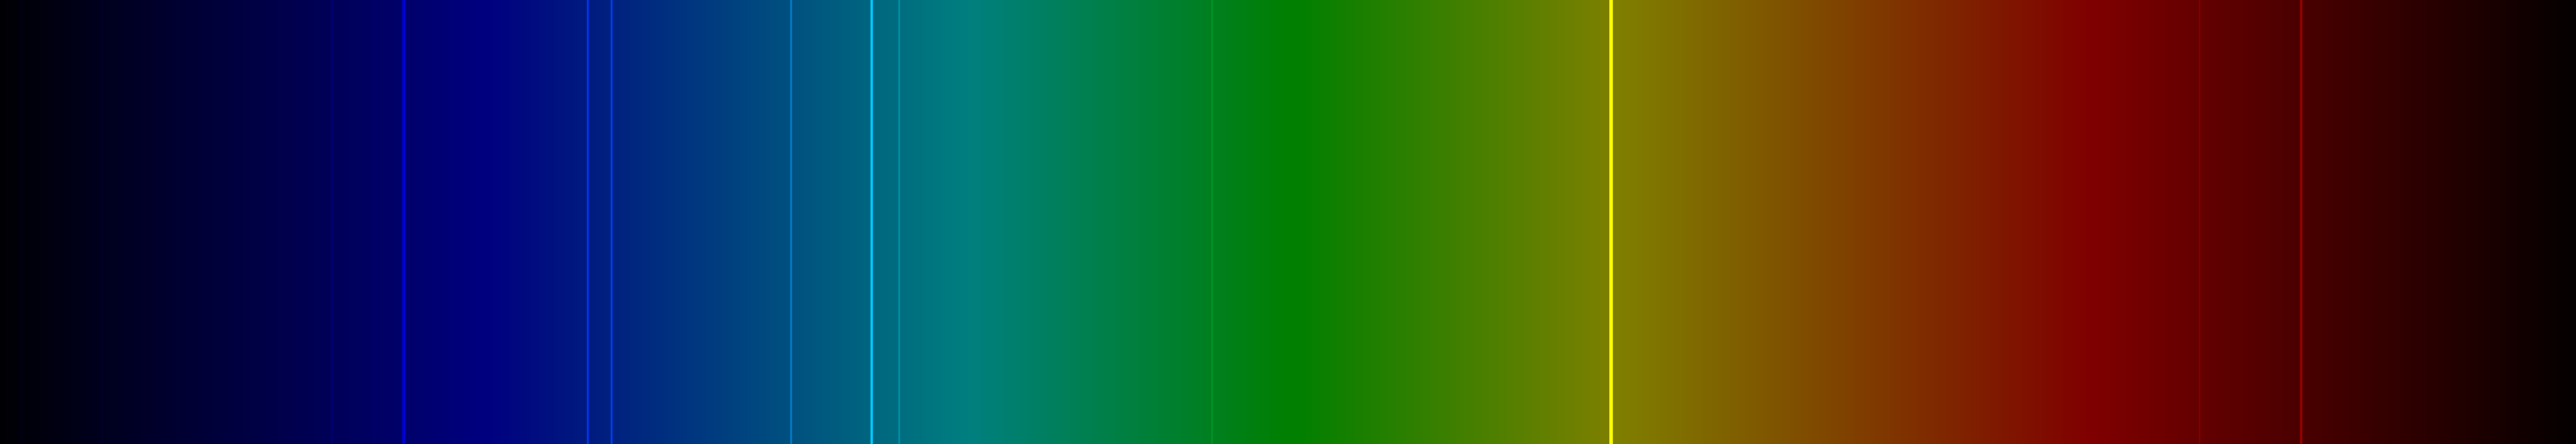
\includegraphics[width=\textwidth, height=0.5cm]{figures/Helium_spectrum_visible}
      \begin{block}{Liouville equation (rotating frame)}
        \begin{gather*}
          \dv{\tilde{\rho}}{t} = -\frac{i}{\hbar} \commutator{\hat{U}\hat{\oper{H}}\hat{U}^\dagger - i\hbar \hat{V}}{\tilde{\rho}} - \hat{\oper{D}}\qty[\tilde{\rho}]; \quad \hat{U} = \mathrm{diag}(1, e^{i \omega_L t}), \quad \hat{V} = \hat{U} \dv{\hat{U}}{t}
        \end{gather*}
      \end{block}

      \begin{gather*}
        \tilde{\mathfrak{F}}\{\tilde{\vb{P}}(\vb{r}, t) \} \equiv -k_2 \int_{}
        \qty(\mathrm{I} -  \outerprod{\bar{\vb{r}}}{\bar{\vb{r}}} ) \cdot \frac{\qty(\partial_t^2 \tilde{\vb{P}}(\vb{r}', t_R) + 2 i \omega_L \partial_t \tilde{\vb{P}}(\vb{r}', t_R) - \omega_L^2 \tilde{\vb{P}}(\vb{r}', t_R)) \alert{e^{-i \omega_L \abs{\vb{r} - \vb{r}'}/c}}}{c^2 \abs{\vb{r}-\vb{r}'}} + \\
        \qty(\mathrm{I} - 3\outerprod{\bar{\vb{r}}}{\bar{\vb{r}}} ) \cdot \frac{\qty(\partial_t \tilde{\vb{P}}(\vb{r}', t_R) + i \omega_L \tilde{\vb{P}}(\vb{r}', t_R))\alert{e^{-i \omega_L \abs{\vb{r} - \vb{r}'}/c}}}{c \abs{\vb{r}-\vb{r}'}^2} +
        \qty(\mathrm{I} - 3\outerprod{\bar{\vb{r}}}{\bar{\vb{r}}} ) \cdot \frac{                \tilde{\vb{P}}(\vb{r}', t_R) \alert{e^{-i \omega_L \abs{\vb{r} - \vb{r}'}/c}}}{\abs{\vb{r}-\vb{r}'}^3}
        \, \dd[3]{\vb{r'}}
      \end{gather*}
\end{frame}

\begin{frame}{Solution methodology}
  \begin{enumerate}
    \item Predict $\hat{\mathbf{\rho}}(t + \Delta t)$
      \begin{enumerate}
        \item Map $\hat{\mathbf{\rho}}(t + \Delta t)$ to $\vb{P}(\vb{r}, t + \Delta t)$
      \end{enumerate}
    \item Calculate $\vb{E}(\vb{r}, t + \Delta t) = \mathfrak{F}\qty{\vb{P}(\vb{r}, t + \Delta t)}$
      \begin{itemize}
        \item retardation, interpolation, causality, derivatives
      \end{itemize}
    \item Use $\displaystyle \vb{E}(\vb{r}, t + \Delta t)$ to calculate $\displaystyle \partial_t \hat{\rho} = -\frac{i}{\hbar} \commutator{\hat{\mathcal{H}}\qty\big(\vb{E}(t + \Delta t))}{\hat{\rho}(t + \Delta t)} - \hat{\mathcal{D}}\qty[\hat{\rho}(t + \Delta t)]$
    \item Use $\partial_t \hat{\rho}$ to correct $\hat{\rho}(t + \Delta t)$
  \end{enumerate}

  \begin{block}{Predictor/corrector}
    \begin{equation*}
    \hat{\rho}(t_{m + 1}) \leftarrow \sum_{w = \alert{-1}}^{W - 1} \qty{\mathcal{P}_{w}^{(0)} / \mathcal{C}_{w}^{(0)}} \hat{\rho}(t_{m-w}) + \qty{\mathcal{P}_{w}^{(1)}/ \mathcal{C}_{w}^{(1)}} \, \partial_t \hat{\rho}(t_{m - w}) \qquad
    \end{equation*}
  \end{block}
\end{frame}

\begin{frame}{Determination of the $\Lambda$s}
  \begin{block}{Multipole expansion}
    \begin{equation*}
      \underbrace{\int_{} \psi_i(\vb{r}) (x - x_0)^{m_x} (y - y_0)^{m_y} (z - z_0)^{m_z}}_{Q_{i\vb{m}}} - \sum_{\vb{u} \in C_i} \Lambda_{i \vb{u}} \underbrace{\delta(\vb{r} - \vb{u}) \dd[3]{\vb{r}}}_{W_{\vb{m}\vb{u}}} = 0
    \end{equation*}
  \end{block}
  \begin{columns}
    \column{0.7\textwidth}
      \begin{itemize}
        \item Grid discretization sufficient to recover $k_0 = \omega_0/c$ spatial variation
        \item Instantaneous ``propagation'' from source to grid
        \item Recover $\grad \div \vb{J}$ from $\grad \div Q_{i\vb{m}}$
      \end{itemize}

    \column{0.3\textwidth}
      \begin{block}{Least-squares fit}
        \begin{equation*}
          \sum_{\vb{u} \in C_i} W_{\vb{m}\vb{u}} \Lambda_{i \vb{u}} = Q_{i\vb{m}}
        \end{equation*}
      \end{block}
  \end{columns}
\end{frame}

\end{document}
